% ============================================================================
% ArrowFlow v3 -- Supplementary Material (original article format)
% Same preamble and macros as main.tex (arXiv master lines 1-34). Cross-
% references to the main manuscript (sections, equations, theorem-like
% statements, figures, tables, citations) resolve through xr-hyper, so
% main.tex must be built first; ./build.sh does this. Sections are in
% supplement_sections/.
% ============================================================================
\documentclass[12pt]{article}
\usepackage{amsmath}
\usepackage{graphicx}
\usepackage{algorithm}
\usepackage{algpseudocode}
\usepackage{xr-hyper}  % must precede hyperref; labels are imported below
\usepackage[hidelinks]{hyperref}
\hypersetup{pdftitle={Supplementary Material for ArrowFlow: Training Ranking Filters with Position Votes},pdfauthor={Ozgur Yilmaz}}
% Long URLs may break after any digit or lowercase letter and stretch slightly, so the reference list has no loose
% lines; a line that cannot break within the tolerance (ArrowFlow is never hyphenated) may stretch a little more.
\makeatletter
\g@addto@macro{\UrlBreaks}{\do\0\do\1\do\2\do\3\do\4\do\5\do\6\do\7\do\8\do\9\do\a\do\b\do\c\do\d\do\e\do\f\do\g\do\h\do\i\do\j\do\k\do\l\do\m\do\n\do\o\do\p\do\q\do\r\do\s\do\t\do\u\do\v\do\w\do\x\do\y\do\z}
\makeatother
\setlength{\emergencystretch}{1.5em}
\Urlmuskip=0mu plus 1mu
\usepackage{natbib}
\usepackage{amsthm}
\usepackage{amssymb}
\usepackage{booktabs}
\usepackage{enumitem}
\usepackage{bm}
\usepackage{multirow}
\usepackage[section]{placeins}  % floats stay inside their own section
\usepackage[margin=1in]{geometry}
\usepackage{tikz}
\usepackage{pgfplots}
\pgfplotsset{compat=1.17}
\usetikzlibrary{arrows.meta, positioning, calc, patterns, decorations.pathreplacing, backgrounds, fit, shapes.geometric, matrix}

% As in main.tex: take the bullet of itemize (and the centered asterisk) from the OMS encoding, so it prints as a bullet.
\DeclareTextSymbolDefault{\textbullet}{OMS}
\DeclareTextSymbolDefault{\textasteriskcentered}{OMS}
\hyphenation{ArrowFlow}
\newcommand{\R}{\mathbb{R}}
\newcommand{\Z}{\mathbb{Z}}
\newcommand{\E}{\mathbb{E}}
\newcommand{\norm}[1]{\left\lVert #1 \right\rVert}
\newcommand{\argsort}{\mathrm{argsort}}
\newcommand{\orderdesc}{\mathrm{argsort}_{\downarrow}}
\newcommand{\rankop}{\mathrm{rank}}
\newcommand{\softmax}{\mathrm{softmax}}

\newtheorem{theorem}{Theorem}
\newtheorem{lemma}[theorem]{Lemma}
\newtheorem{corollary}[theorem]{Corollary}
\newtheorem{proposition}[theorem]{Proposition}
\newtheorem{definition}[theorem]{Definition}
\newtheorem{remark}{Remark}

% Import the main manuscript's labels AFTER the custom macros above, since the
% main .aux references them inside hyperref label metadata (same mechanism as
% the Neural Computation supplement, manuscript/NeuralComputation/submission/;
% xr-hyper itself is loaded before hyperref in the package list, as it requires).
% The links to main-text labels open main.pdf by file name: keep the names main.pdf and supplement.pdf in a
% submission bundle.
\externaldocument[][nocite]{main}

% Number supplementary sections, tables, figures, equations and theorem-like
% statements with an "S" prefix.
\renewcommand{\thesection}{S\arabic{section}}
\renewcommand{\thesubsection}{S\arabic{section}.\arabic{subsection}}
\renewcommand{\thetable}{S\arabic{table}}
\renewcommand{\thefigure}{S\arabic{figure}}
\renewcommand{\theequation}{S\arabic{equation}}
\renewcommand{\thetheorem}{S\arabic{theorem}}
\renewcommand{\theremark}{S\arabic{remark}}

\begin{document}

\title{Supplementary Material\\[2pt]\large ArrowFlow: Training Ranking Filters with Position Votes}
\author{Ozgur Yilmaz \\
\small Department of Artificial Intelligence\\
\small Adana Science and Technology University, Adana, Turkey}
\date{}
\maketitle

% Navigation: a table of contents and a list of tables. Every supplement caption opens with a bold title, and the list
% shows only that title: inside this group, \numberline passes on the table number and keeps the argument of the first
% \textbf of the caption (the whole caption if it has none). A wider page-number box keeps a long title clear of a
% three-digit page number.
\tableofcontents
\begingroup
\makeatletter
\renewcommand*{\@pnumwidth}{2.2em}
\let\sm@numberline\numberline
\def\sm@lottitle#1\textbf#2#3\sm@end{\ifx\relax#2#1\else#2\fi}
\renewcommand{\numberline}[2]{\sm@numberline{#1}\sm@lottitle#2\textbf\relax\sm@end}
\makeatother
\listoftables
\endgroup
\clearpage

\section{Proofs}\label{supp:proofs}

This section proves the statements of Sections~\ref{sec:arrow} and~\ref{sec:theory} of the main text, in the order in which they appear, and adds the worked examples they refer to. None of these results is a convergence or generalization theorem for the trained network. Section~\ref{sec:theory} states several results only in words. Three of them receive exact statements as propositions below, and the subsections on the alphabet, the angle and the batch update prove the others. Each subsection is headed with the part of Section~\ref{sec:theory} it supports. Positions are counted from $1$, and the implementation counts from $0$. Adding one to every position changes no ordering, no footrule distance and no aggregate in exact arithmetic, because position sums shift by a common constant.

\subsection{Details for Section~\ref*{sec:arrow}: The Update Rule and Arrow's Axioms}\label{supp:iia}

Every update of a ranking filter merges several rankings into one, so it can be studied with Arrow's impossibility theorem. The weighted Borda count is Pareto efficient and non-dictatorial under the weight condition of Proposition~\ref{prop:borda-iia}, so by Arrow's theorem it violates independence of irrelevant alternatives (IIA). This subsection proves the proposition. It also gives witnesses, small examples on which the violation can be checked by hand. Last, it treats the update as training runs it, with the filter's current order held fixed.

A profile lists one ranking per voter, and two profiles are compared voter by voter. The three axioms are those of Section~\ref{sec:arrow}. Pareto efficiency asks that the collective ranking place $a$ before $b$ whenever every voter does. Non-dictatorship asks that no single voter's ranking be the collective ranking on every profile. IIA asks that the collective order of $a$ and $b$ depend only on how each voter orders $a$ and $b$, so that moving a third item on the ballots cannot change it.

The rule under study is the weighted Borda count~\eqref{eq:borda-update}. With fixed positive weights $\omega_i$, item $v$ receives the score $P(v)=\sum_i\omega_i\operatorname{pos}_{\pi_i}(v)$ over the voters $i$. The collective ranking sorts the items by $P$, with ties broken by the fixed item order. When a batch update is read as an election (Section~\ref{sec:arrow}), the prior $r_j$ has weight one and voter $t$ has weight $\omega_t=|a_t|$.

\begin{proof}[Proof of Proposition~\ref{prop:borda-iia}]
\emph{Universal domain.} $P$ is defined for every profile of complete rankings, so the rule returns a ranking on every profile.

\emph{Pareto.} If every voter places $a$ before $b$, then $\operatorname{pos}_{\pi_i}(a)<\operatorname{pos}_{\pi_i}(b)$ for every $i$. Multiplying by $\omega_i>0$ and summing gives $P(a)<P(b)$, so $a$ precedes $b$ whatever the tie rule.

\emph{Non-dictatorship.} Fix a voter $i$ and let $\Omega_{-i}$ be the combined weight of the other voters. By assumption, $\omega_i\le(V-1)\Omega_{-i}$. Take two items $a$ and $b$, with $a$ the one of higher identifier (ID). Consider the profile in which voter $i$ places $a$ first and $b$ second, while every other voter places $b$ first and $a$ last. Then
\[
P(b)-P(a)=\omega_i(2-1)+\sum_{i'\neq i}\omega_{i'}(1-V)=\omega_i-(V-1)\Omega_{-i}\le0.
\]
So either $b$ precedes $a$ strictly, or the two tie. In a tie, the tie rule puts the lower ID first, and that is $b$. In both cases the collective ranking disagrees with voter $i$, so no voter is a dictator.

\emph{IIA.} Arrow's theorem \citep{arrow1963social} concerns rules on profiles of rankings of at least three alternatives. It states that such a rule with universal domain that satisfies Pareto and is non-dictatorial cannot satisfy IIA. The witnesses below show the violation directly.
\end{proof}

The weight condition is exact. A voter that weighs more than $V-1$ times all others combined is a dictator. Whenever it places $a$ before $b$, $P(b)-P(a)\ge\omega_i-(V-1)\Omega_{-i}>0$. For the prior, whose weight is one, this happens when the total vote weight of the batch is below $1/(V-1)$. Such a batch cannot move the filter. How often a batch reaches this weight in training is reported only for the first of two hidden layers under the corrected relay. There, 58.4 percent of the filter-batches with a nonzero vote reached it on average, and 97.7 percent when these votes were multiplied by 8 (Table~\ref{tab:s-relay-movement}).

\paragraph{Witness without the prior.}
Take three items $a,b,c$ and two voters of weight one. A ballot $abc$ places $a$ first, $b$ second and $c$ third. Compare the profiles
\[
\Pi=(abc,\;bca)\qquad\text{and}\qquad\Pi'=(acb,\;bac).
\]
In both, voter 1 places $a$ before $b$ and voter 2 places $b$ before $a$. Only the position of $c$ relative to $a$ and $b$ changes. The position sums $(P(a),P(b),P(c))$ are $(4,3,5)$ for $\Pi$, giving $bac$, and $(3,4,5)$ for $\Pi'$, giving $abc$. The order of $a$ and $b$ reverses strictly, so the tie rule plays no part. Moving $c$ alone thus reverses the collective order of $a$ and $b$, which IIA forbids.

\paragraph{Witness with the prior.}
The same happens with a prior. Take the prior $r=abc$ with weight one and six votes of weight $\tfrac12$, and compare the profiles
\[
\widetilde\Pi=(abc,abc,abc,bca,bca,bca)\qquad\text{and}\qquad\widetilde\Pi'=(acb,acb,acb,bac,bac,bac).
\]
Every corresponding voter keeps its order of $a$ and $b$, and the prior and weights are identical. The position sums are $(7,\tfrac{13}{2},\tfrac{21}{2})$ for $\widetilde\Pi$, giving $bac$, and $(\tfrac{11}{2},8,\tfrac{21}{2})$ for $\widetilde\Pi'$, giving $abc$. Dividing by the total weight $4$ gives the mean voted positions of~\eqref{eq:rowmean-borda}. The weight condition holds, since $1<2\cdot3$ for the prior and $\tfrac12<2\cdot\tfrac72$ for each vote.

Both witnesses concern the aggregation rule with fixed voters and weights. In training, the accepted targets and their weights depend on the current predictions and on representations that change from batch to batch. And no vote from an earlier batch is retained. The witnesses therefore show what the rule does on such profiles. They do not show that such profiles arise in training, and they imply nothing about classification accuracy.

\paragraph{The domain of the proposition.} The proposition varies every ballot, the prior included. One update, however, holds the prior fixed. The map from the remaining ballots is then defined on every profile of those ballots, so by Arrow's theorem it cannot satisfy all three axioms either. Which axioms it gives up depends on the total vote weight $\Omega$ of the batch, and there are three cases (Figure~\ref{fig:s-weight-regimes}). If $\Omega<1/(V-1)$, the current order decides alone and the map is constant. The constant map satisfies IIA, and no ballot dictates, but it is not Pareto efficient.

If $1/(V-1)<\Omega<V-1$, the map is not Pareto efficient. Take items $a$ and $b$ at the two ends of the prior, and let every ballot place $b$ immediately before $a$. Then $P(b)-P(a)=(V-1)-\Omega>0$. Arrow's theorem, which assumes Pareto efficiency, then says nothing about IIA. But IIA fails directly, so here the map gives up both Pareto efficiency and IIA. Take two items with $a$ before $b$ in the prior, $g$ positions apart, where $\Omega<g<(V-1)\Omega$. For example, $g=1$ works if $\Omega<1$, and $g=\lfloor\Omega\rfloor+1$ otherwise. If every ballot places $b$ immediately before $a$, then $P(b)-P(a)=g-\Omega>0$ and the filter keeps $a$ first. If every ballot places $b$ first and $a$ last, then $P(b)-P(a)=g-(V-1)\Omega<0$ and the filter places $b$ first. Yet no ballot changed its order of $a$ and $b$.

At $V=3$ with $\Omega=1$ this construction fails, because no such $g$ exists, but IIA still fails through the tie rule. Take the prior $abc$, which is also the identifier order, and one ballot of weight one. The ballots $cba$ and $cab$ both place $c$ before $b$. The first gives the position sums $(4,4,4)$, and the tie rule keeps $b$ before $c$. The second gives $(3,5,4)$ and places $c$ before $b$. For every other identifier order, one of the three pairs of the prior gives a witness of the same kind.

If $\Omega>V-1$, the map is Pareto efficient. Unless one ballot outweighs $V-1$ times all other weight, the prior's included, it violates IIA by Arrow's theorem, as the six-vote witness above does with its prior fixed.

At each boundary between these cases the tie rule decides. For example, take $V=3$ and the prior $abc$ of weight one, which is also the identifier order. Add one vote of weight $\tfrac12$, so that $\Omega=1/(V-1)$. Every pair of items keeps a score gap of at least $1-2\cdot\tfrac12=0$ in the order of the prior, and an equality goes to the identifier order. So each of the six possible ballots returns $abc$. This map is constant. It satisfies IIA, and no ballot dictates. But it is not Pareto efficient, since the ballot $cba$ places $c$ before $a$ and the output does not. With a prior that disagrees with the identifier order, the update can move the filter at this boundary. It can do so only through a tie, because every pair keeps a score gap of at least $1-(V-1)\Omega=0$ in the order of the prior. Such a prior has two neighbors, $a$ just before $b$, with $b$ of lower identifier. If every ballot places $b$ first and $a$ last, then $P(b)-P(a)=1-(V-1)\Omega=0$, and the tie rule puts $b$ first. If every ballot places $b$ immediately before $a$, then $P(b)-P(a)=1-\Omega>0$ and $a$ stays first. So IIA fails at this boundary too.

In ArrowFlow's layers each vote weighs less than $2\eta\le0.4$ and a batch has $32$ examples, so $\Omega<12.8<15\le V-1$. No update is therefore Pareto efficient, and an update that can move its filter violates IIA by the constructions above.

% Figure: the three weight ranges of one update with the prior fixed (supplement, Section S1.1). Drawn by hand; it
% restates the cases of the paragraph "The domain of the proposition" (not to scale).
\begin{figure}[!htbp]
\centering
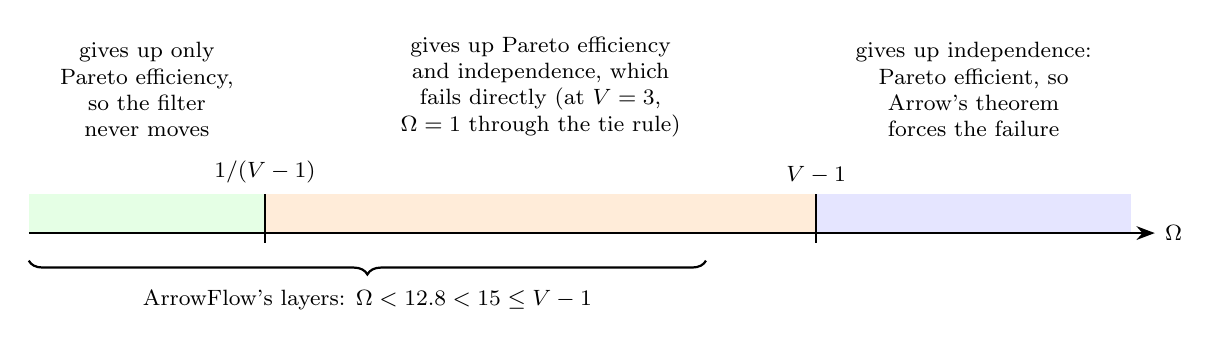
\begin{tikzpicture}[
    >=Stealth,
    lbl/.style={font=\footnotesize, align=center},
    tick/.style={font=\footnotesize},
]
\fill[green!10] (0,0) rectangle (3,0.5);
\fill[orange!15] (3,0) rectangle (10,0.5);
\fill[blue!10] (10,0) rectangle (14,0.5);
\draw[->, thick] (0,0) -- (14.3,0) node[right, font=\footnotesize] {$\Omega$};
\draw[thick] (3,-0.12) -- (3,0.5) node[above, tick] {$1/(V-1)$};
\draw[thick] (10,-0.12) -- (10,0.5) node[above, tick] {$V-1$};
\node[lbl, anchor=south] at (1.5,1.1) {gives up only\\Pareto efficiency,\\so the filter\\never moves};
\node[lbl, anchor=south] at (6.5,1.1) {gives up Pareto efficiency\\and independence, which\\fails directly (at $V=3$,\\$\Omega=1$ through the tie rule)};
\node[lbl, anchor=south] at (12,1.1) {gives up independence:\\Pareto efficient, so\\Arrow's theorem\\forces the failure};
\draw[decorate, decoration={brace, mirror, amplitude=5pt}, thick] (0,-0.35) -- (8.6,-0.35)
      node[midway, below=7pt, lbl] {ArrowFlow's layers: $\Omega<12.8<15\le V-1$};
\end{tikzpicture}
\caption{\textbf{What one update gives up when the current order is held fixed.} One batch update of a filter over $V$ items depends on the total vote weight $\Omega$ of the batch, drawn here on an axis that is not to scale. Below $1/(V-1)$ the current order decides alone, so the update never moves the filter. This constant map satisfies independence of irrelevant alternatives, and no ballot dictates, but it is not Pareto efficient. Between $1/(V-1)$ and $V-1$ the update gives up both Pareto efficiency and independence. Independence fails directly by the construction in this subsection, and at $V=3$ with $\Omega=1$ through the tie rule. Figure~\ref{fig:iia} of the main text shows a case from this middle range. Above $V-1$ the update is Pareto efficient, and Arrow's theorem forces the failure unless one ballot outweighs $V-1$ times all other weight, the prior's included. In ArrowFlow's layers every update lies in the first two ranges. At each boundary the tie rule decides.}
\label{fig:s-weight-regimes}
\end{figure}


\paragraph{The forward pass.} Section~\ref{sec:arrow} observes that the forward pass orders any two filters of a layer independently of the other filters. This is not Arrow's independence axiom, because the forward pass aggregates no profile of rankings.

\subsection{Score-Gap Stability}

This subsection proves Proposition~\ref{prop:score-stability}. If every score moves by less than half the smallest gap between two scores, the encoded ranking stays the same. The proof is short, because the score-gap condition bounds the change in every pairwise difference of the scores at once.

\begin{proof}[Proof of Proposition~\ref{prop:score-stability}]
Take any pair with $z_i<z_j$. Then
\[
(z_j+\varepsilon_j)-(z_i+\varepsilon_i)\ge z_j-z_i-2\|\varepsilon\|_\infty\ge\delta_{\min}(z)-2\|\varepsilon\|_\infty>0 .
\]
Every strict pairwise order is preserved, so the sorted order of the coordinates, and with it $\argsort$, is unchanged. The strict inequality in the hypothesis rules out a perturbation that creates a tie.
\end{proof}

\subsection{Details for Section~\ref*{sec:theory-stability}: Gaussian Perturbation through an Affine Encoder}\label{supp:gaussian}

Under Gaussian noise the score-gap condition cannot hold for sure, because Gaussian noise exceeds any bound with positive probability. This subsection therefore bounds the probability that Gaussian noise on the input changes the encoded ranking. Section~\ref{sec:theory-stability} summarizes this result in words. For an encoder of degree one the scores are affine in the input, that is, a linear function of it plus a constant. So Gaussian input noise stays Gaussian at the score level.

\begin{proposition}[Gaussian perturbation through an affine encoder]\label{prop:gaussian-stability}
Let $z_i(x)=w_i^{\top}x+b_i$ for $i=1,\dots,e$, with any fitted standardization folded into $w_i$ and $b_i$. Assume that $z(x)$ has distinct coordinates. Let $\varepsilon\sim\mathcal N(0,\Sigma)$ with $\Sigma$ positive semidefinite, and put $\delta_{ij}=|z_i(x)-z_j(x)|$ and $v_{ij}=(w_i-w_j)^{\top}\Sigma\,(w_i-w_j)$. Then
\begin{equation}\label{eq:gaussian-pair-bound}
\Pr\bigl[\argsort(z(x+\varepsilon))\neq\argsort(z(x))\bigr]
\le\min\Bigl\{1,\;\sum_{i<j,\;v_{ij}>0}\Phi_{\mathcal N}\bigl(-\delta_{ij}/\sqrt{v_{ij}}\bigr)\Bigr\},
\end{equation}
where $\Phi_{\mathcal N}$ is the standard normal distribution function, and a pair with $v_{ij}=0$ contributes zero.
\end{proposition}

The bound uses each pair's own gap and variance, and it allows correlated input noise. Each pair of scores reverses with a normal tail probability, and the union bound combines the pairs. The union bound says that the probability that at least one of several events occurs is at most the sum of their probabilities. The last paragraph of this subsection shows that the sum is also the expected Kendall distance between the clean and perturbed rankings. The Kendall distance counts the pairs that two rankings order differently.

\begin{proof}[Proof of Proposition~\ref{prop:gaussian-stability}]
Since $z_i(x+\varepsilon)=z_i(x)+w_i^{\top}\varepsilon$, a pair with $z_i(x)<z_j(x)$ has the perturbed difference $\delta_{ij}+(w_j-w_i)^{\top}\varepsilon$. Its random part is a normal variable with mean zero and variance $v_{ij}$. If $\argsort$ changes, some pair that is strictly ordered at $x$ is reversed or tied at $x+\varepsilon$. For a pair with $v_{ij}>0$ the reversal has probability $\Phi_{\mathcal N}(-\delta_{ij}/\sqrt{v_{ij}})$ and the tie has probability zero. For a pair with $v_{ij}=0$ the random part vanishes almost surely, that is, with probability one, so neither can happen. The union bound over the pairs gives the sum in~\eqref{eq:gaussian-pair-bound}, and a probability is at most one. The union bound needs no independence between pairs.
\end{proof}

For isotropic noise, which has the same variance in every direction, $\Sigma=\sigma^2I$ gives $v_{ij}=\sigma^2\|w_i-w_j\|_2^2$. Treating the projected coordinates as independent would give a different variance and is unnecessary.

\paragraph{The sum as an expected distance.} Let $S$ be the sum of pair probabilities in~\eqref{eq:gaussian-pair-bound}, before the cap at one. Each of its terms is exactly the probability that its pair reverses. A reversed pair is a pair that the clean and perturbed rankings order differently. By linearity of expectation, $S$ is therefore the expected Kendall distance $\E[d_K]$ between the two rankings, and $d_F\le2d_K$ \citep{diaconis1977footrule} gives $\E[d_F]\le2S$. This extends the bound to the first ranking layer. Suppose the responses of a first ranking layer at $\pi_x$, the footrule distances from $\pi_x$ to the layer's filters, are distinct, with smallest consecutive gap $g_{\min}$. By Proposition~\ref{prop:layer-margin}(ii) and Markov's inequality, the layer keeps its output ordering at $x+\varepsilon$ except with probability at most $4S/g_{\min}$. Markov's inequality bounds the probability that a nonnegative variable is at least some level by its mean divided by that level. A changed output also needs a changed encoding, so the probability that the output changes is at most $\min\{1,S,4S/g_{\min}\}$. At the layer sizes used here, however, the responses are rarely all distinct (Section~\ref{supp:margin}). Without that condition the bound is $\min\{1,S\}$, the bound for the encoding itself.

\subsection{Local Sensitivity of Polynomial Encoders}\label{supp:poly}

The bound of Section~\ref{supp:gaussian} needs an encoder of degree one, whose scores are affine in the input. An encoder of higher degree makes each score a polynomial in the input. This subsection shows that for small noise the variance of a change in a score difference is still set, to leading order, by the gradient of that difference.

Let $f\colon\R^d\to\R^e$ be a fitted encoder of degree $p$, the composition of polynomial expansion, standardization and projection, so that each score $f_i$ is a polynomial in $x$. Fix $x$ and a positive semidefinite matrix $\Sigma_0$, and let $\varepsilon=\sigma\zeta$ with $\zeta\sim\mathcal N(0,\Sigma_0)$. For the score difference $\Delta_{ij}(x)=f_i(x)-f_j(x)$,
\begin{equation}\label{eq:poly-local}
\operatorname{Var}\bigl[\Delta_{ij}(x+\varepsilon)-\Delta_{ij}(x)\bigr]=\sigma^2\,\nabla\Delta_{ij}(x)^{\top}\Sigma_0\,\nabla\Delta_{ij}(x)+O(\sigma^4)\qquad(\sigma\to0),
\end{equation}
where the constant in the remainder may depend on $x$, $f$ and $\Sigma_0$.

\begin{proof}
The polynomial $\Delta_{ij}$ has a finite Taylor expansion,
\[
\Delta_{ij}(x+\sigma\zeta)-\Delta_{ij}(x)=\sigma\,\nabla\Delta_{ij}(x)^{\top}\zeta+\sigma^2 q_2(\zeta)+\sigma^3 q_3(\zeta)+\dots,
\]
with $q_2$ homogeneous quadratic, $q_3$ homogeneous cubic and finitely many further terms of higher degree in $\zeta$. A homogeneous polynomial is one whose terms all have the same total degree. The variance of the linear term is the quadratic form in~\eqref{eq:poly-local}. Its covariance with $q_2(\zeta)$ vanishes. Because $q_2$ is homogeneous of degree two, its product with the linear term is homogeneous of degree three. And every moment of odd total degree of a Gaussian vector with mean zero is zero. Every remaining contribution to the variance is of order $\sigma^4$ or higher in $\sigma$, and all Gaussian moments are finite.
\end{proof}

The gradient in~\eqref{eq:poly-local} is built from the derivatives of monomials. For a monomial $x^{\alpha}=\prod_i x_i^{\alpha_i}$, a product of powers of the features, the derivative with respect to $x_i$ is
\[
\frac{\partial x^{\alpha}}{\partial x_i}=\alpha_i\,x_i^{\alpha_i-1}\prod_{i'\neq i}x_{i'}^{\alpha_{i'}}
\]
when $\alpha_i>0$ and zero otherwise. The expression covers repeated powers and does not divide by $x_i$, so it is defined at zero. For example, $x_i^{p}$ has derivative $p\,x_i^{p-1}$. The gradient of a score difference combines these derivatives with the fitted standardization and projection coefficients. So the sensitivity of a single monomial before projection is not enough to describe that of a score.

Equation~\eqref{eq:poly-local} is a local variance expansion, valid for small noise. A nonlinear polynomial of Gaussian noise is generally not Gaussian and may have a nonzero mean shift. So inserting this variance into~\eqref{eq:gaussian-pair-bound} would not give an exact bound for noise of finite size.

\subsection{Details for Section~\ref*{sec:theory-alphabet}: The Ordinal Alphabet and Permutation Cones}\label{supp:alphabet}

This subsection proves the statements of Section~\ref{sec:theory-alphabet} about the alphabet, the set of rankings that the encoder can emit. Ranking keeps order and discards magnitude. Applying one strictly increasing function to every coordinate leaves $\argsort(z)$ unchanged. This holds for the vector that is sorted. It does not hold for raw features transformed before expansion and projection. For scores without ties, $\argsort(z)$ takes one of $e!$ values, so the entropy of the encoded ranking obeys
\begin{equation}\label{eq:alphabet}
H(\pi_x)\le\log_2(e!),
\end{equation}
with equality only when all $e!$ orderings are equally likely.

All score vectors without ties that share one ranking form a cone (Figure~\ref{fig:cones} of the main text). The encoding is constant inside a cone and jumps at its walls. Each ranking layer sorts distances, so it is piecewise constant too. A fixed projection may land in only some cones, and at degree one their number can be counted (the last paragraph of this subsection). So~\eqref{eq:alphabet} bounds the alphabet and not the information the data carry, and it predicts neither classification error nor network capacity. At fixed $e$, polynomial expansion leaves the bound $e!$ unchanged, but it can enlarge the set of rankings that the encoder reaches. And the preimages of the cones, the sets of inputs that land in each cone, need not be convex. Training the layers that follow a fitted encoder does not move the cone walls. The rest of this subsection proves these statements.

Two score vectors without ties have the same $\argsort$ if and only if $z_i-z_j$ has the same sign in both for every pair $i\neq j$. For a permutation $\pi$ of the $e$ coordinates, the set $\mathcal{C}_\pi=\{z: z_{\pi[1]}<z_{\pi[2]}<\dots<z_{\pi[e]}\}$ is defined by $e-1$ strict linear inequalities, so it is open and convex. It is closed under positive scaling, which makes it a cone. It is also closed under adding a multiple of the all-ones vector. The $e!$ sets $\mathcal{C}_\pi$ are pairwise disjoint. The union of the hyperplanes $\{z_i=z_j\}$ has Lebesgue measure zero, that is, zero volume, and its complement is the union of the cones. Since $\argsort$ is constant on each $\mathcal{C}_\pi$ and takes different values on different cones, the encoded ranking takes at most $e!$ values. The entropy of a random variable with at most $e!$ values is at most $\log_2(e!)$, with equality exactly when all $e!$ values are equally likely. This is~\eqref{eq:alphabet}. It remains to show that a strictly increasing function leaves $\argsort(z)$ unchanged. Such a function preserves every strict inequality and every equality between coordinates. So all pairwise comparisons are unchanged, and therefore so are the sorted order and the tie rule's decisions.

\paragraph{The rankings a view reaches at degree one.} At degree one the scores of every view are linear in the standardized features $q\in\R^d$, with no offset (Section~\ref{supp:encoder}). So each score is $z_i=q^{\top}w_i$ for a fitted vector $w_i\in\R^d$. The encoded ranking is then the order in which the linear function $w\mapsto q^{\top}w$ sorts the $e$ points $w_1,\dots,w_e$ of $\R^d$. \citet{cover1967orderings} counted such orders. For $e$ points in general position in $\R^d$, linear functions induce exactly $Q(e,d)$ orders, where $Q(1,d)=1$, $Q(e,1)=2$ for $e\ge2$, and $Q(e+1,d)=Q(e,d)+e\,Q(e,d-1)$ for $d\ge2$. Points in other positions give at most as many. The columns of a Gaussian matrix are in general position with probability one, so a random view reaches all $Q(e,d)$ orders as $q$ ranges over $\R^d$. For $e=16$ and $d=4$ that is $437{,}040$ rankings, against $16!\approx2.1\times10^{13}$. A polynomial expansion makes the scores linear in more coordinates, which raises this bound.

\subsection{Angle Property of the Random Projection}\label{supp:angle}

For the random projection strategy, the expected disagreement between the rankings of two inputs is set by the angle between their expanded, standardized feature vectors. So inputs that point in similar directions get similar rankings on average. This subsection states and proves the exact relation.

Let $q,q'\in\R^{d'}$ be the two feature vectors, both nonzero, with angle $\theta\in[0,\pi]$. Let $W\in\R^{d'\times e}$, $e\ge2$, have independent standard normal entries. Put $\kappa=\argsort(qW)$ and $\kappa'=\argsort(q'W)$. Let $d_K(\kappa,\kappa')$ be the Kendall distance \citep{kendall1938}, the number of coordinate pairs that the two rankings order differently. Then
\begin{equation}\label{eq:angle}
\E\bigl[d_K(\kappa,\kappa')\bigr]=\binom{e}{2}\frac{\theta}{\pi},\qquad \binom{e}{2}\frac{\theta}{\pi}\le\E\bigl[d_F(\kappa,\kappa')\bigr]\le2\binom{e}{2}\frac{\theta}{\pi}.
\end{equation}

\begin{proof}
Fix coordinates $i<j$ and let $g$ be column $i$ of $W$ minus column $j$, so $g\sim\mathcal N(0,2I)$. The score difference of the pair is then $q^{\top}g$ for $q$ and $q'^{\top}g$ for $q'$. Since $q\neq0$, $q^{\top}g$ is a normal variable with mean zero and positive variance, so the pair ties with probability zero. The same holds for $q'$, so the tie rule plays no part almost surely. The pair is ordered differently exactly when $q^{\top}g$ and $q'^{\top}g$ have opposite signs. If $q'$ is a positive multiple of $q$, the two rankings agree and $\theta=0$. If it is a negative multiple, every pair is reversed and $\theta=\pi$. The formula holds in both cases. Otherwise $q$ and $q'$ span a plane, and we project $g$ onto it. The projection is an isotropic Gaussian vector of that plane, so its direction is uniform on the circle. And only the projection enters $q^{\top}g$ and $q'^{\top}g$. The two signs differ when the line orthogonal to the projection separates $q$ and $q'$. This happens on two arcs of total angle $2\theta$ out of $2\pi$ (Figure~\ref{fig:s-angle}), so with probability $\theta/\pi$ \citep{charikar2002similarity}. Summing over the $\binom{e}{2}$ pairs gives the expected Kendall distance by linearity of expectation, which needs no independence between pairs. Every two rankings satisfy $d_K\le d_F\le2d_K$ \citep{diaconis1977footrule}, and taking expectations gives the bounds.
\end{proof}

% Figure: why a coordinate pair flips with probability theta/pi (supplement, Section S1.6). Drawn by hand; q at angle 0,
% q' at theta = 50 degrees; g flips the pair when it points into (90, 90+theta) or (270, 270+theta) degrees.
\begin{figure}[!htbp]
\centering
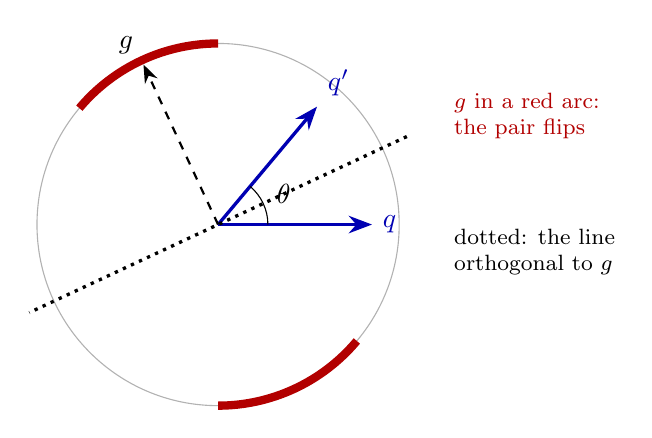
\begin{tikzpicture}[>=Stealth, scale=1.15]
\def\th{50}
\draw[black!30] (0,0) circle (2);
% the two arcs of directions of g that separate q and q'
\draw[red!70!black, line width=3pt] (90:2) arc (90:90+\th:2);
\draw[red!70!black, line width=3pt] (270:2) arc (270:270+\th:2);
% q and q'
\draw[->, very thick, blue!70!black] (0,0) -- (0:1.7) node[right] {$q$};
\draw[->, very thick, blue!70!black] (0,0) -- (\th:1.7) node[above right] {$q'$};
\draw (0:0.55) arc (0:\th:0.55);
\node at (\th/2:0.8) {$\theta$};
% one direction of g inside an arc, and the line orthogonal to it
\draw[->, thick, dashed] (0,0) -- (115:1.95) node[above left] {$g$};
\draw[dotted, very thick] (25:2.3) -- (205:2.3);
\node[font=\footnotesize, align=left, anchor=west, red!70!black] at (2.5,1.2) {$g$ in a red arc:\\the pair flips};
\node[font=\footnotesize, align=left, anchor=west] at (2.5,-0.3) {dotted: the line\\orthogonal to $g$};
\end{tikzpicture}
\caption{\textbf{Why a pair of coordinates flips with probability $\theta/\pi$.} The plane spanned by the two feature vectors $q$ and $q'$, which form the angle $\theta$. The projection of the random direction $g$ onto this plane points in a uniformly random direction. The pair is ordered differently for $q$ and $q'$ exactly when the line orthogonal to $g$ (dotted) separates $q$ from $q'$. That happens when $g$ points into one of the two red arcs. The arcs have total angle $2\theta$ out of $2\pi$, so the pair flips with probability $\theta/\pi$. The dashed arrow shows one such $g$.}
\label{fig:s-angle}
\end{figure}


Kendall's rank correlation $\tau$ between two rankings of $e$ items is $1-2d_K/\binom{e}{2}$. So in expectation over $W$, for fixed inputs, $\E[\tau(\kappa,\kappa')]=1-2\theta/\pi$. This is the arcsine kernel of the two feature vectors. It equals twice the arc-cosine kernel of order 0 defined by \citet{cho2009kernel}, minus one. The Kendall kernel of the support vector classifier in Section~\ref{supp:controlled} is this $\tau$, computed for the one projection that each view draws.

The property concerns the random strategy only. The target-aware projection places discriminant coordinates fitted to the labels, and the calibrated projection standardizes the projected coordinates with training statistics. The property holds for each view separately and says nothing about the trained layers above the encoder.

\subsection{Details for Section~\ref*{sec:theory-margin}: Fixed-Layer Margin}\label{supp:margin}

This subsection asks how far an input ranking can move before a fixed ranking layer changes its output. The answer is a margin, much like the score-gap condition of the encoder. A fixed layer with filters $r_1,\dots,r_N$ over $V$ items orders its filters by their responses $D_j=d_F(\pi,r_j)$ to the input $\pi$. Since the footrule is a metric, no response changes by more than the input moves. So, when the responses are distinct, the smallest gap between consecutive responses guarantees the same output for every input in a ball around $\pi$. When responses tie, a second bound at the end of this subsection limits how far the output can move.

\begin{proposition}[Fixed-layer margin]\label{prop:layer-margin}
Let $\pi$ and $\pi'$ be rankings of the $V$ items of a layer with filters $r_1,\dots,r_N$, $N\ge2$.
\begin{enumerate}[label=(\roman*),nosep]
\item For every filter, $|d_F(\pi,r_j)-d_F(\pi',r_j)|\le d_F(\pi,\pi')$.
\item If the responses at $\pi$ are distinct with smallest consecutive gap $g_{\min}$ and $d_F(\pi,\pi')<g_{\min}/2$, the output ordering at $\pi'$ equals that at $\pi$. If only the two smallest responses are separated, by $g_1>0$, then $d_F(\pi,\pi')<g_1/2$ preserves the nearest filter.
\item If the responses at $\pi$ are distinct, let $\Delta^*(\pi)$ be the smallest footrule distance from $\pi$ to an input with a different output ordering. Then $g_{\min}/2\le\Delta^*(\pi)\le D_{(2)}$, with $D_{(2)}$ the second-smallest response.
\end{enumerate}
\end{proposition}

The lower bound is a certified radius, a distance within which the output is guaranteed not to change. The upper bound says that a layer with two distinct filters can always be moved off its output. Under the prototype readout the nearest output filter is the predicted class, so the second part of (ii) is that readout's classification margin. All three parts follow from the reverse triangle inequality of the footrule metric. This inequality says that the distances from two inputs to one filter differ by at most the distance between the inputs.

\begin{proof}[Proof of Proposition~\ref{prop:layer-margin}]
\emph{(i)} This is the reverse triangle inequality for the metric $d_F$,
\[
d_F(\pi,r_j)\le d_F(\pi,\pi')+d_F(\pi',r_j),
\]
together with the same inequality with $\pi$ and $\pi'$ exchanged.

\emph{(ii)} Let $d_F(\pi,\pi')<g_{\min}/2$. For two filters $j$ and $j'$ with $D_j(\pi)<D_{j'}(\pi)$ consecutive in the sorted responses, (i) gives
\[
D_{j'}(\pi')-D_j(\pi')\ge\bigl(D_{j'}(\pi)-d_F(\pi,\pi')\bigr)-\bigl(D_j(\pi)+d_F(\pi,\pi')\bigr)\ge g_{\min}-2\,d_F(\pi,\pi')>0 .
\]
Every consecutive pair keeps its strict order, so the whole ordering is unchanged and no tie arises. For the second claim, let $r_{(1)}$ be the nearest filter at $\pi$ with response $D_{(1)}$ and let $g_1=D_{(2)}-D_{(1)}>0$. If $d_F(\pi,\pi')<g_1/2$, then $D_{(1)}(\pi')<D_{(1)}+g_1/2$. Every other filter $j$ has $D_j(\pi')>D_j(\pi)-g_1/2\ge D_{(2)}-g_1/2=D_{(1)}+g_1/2$. So $r_{(1)}$ remains the unique nearest filter.

\emph{(iii)} By (ii), every input within footrule distance $g_{\min}/2$ of $\pi$ has the same output ordering, so $\Delta^*(\pi)\ge g_{\min}/2$. Distinct responses at $\pi$ force pairwise distinct filters, because equal filters have equal responses at every input. For the upper bound, let $r_{(2)}$ be the filter with the second-smallest response and take $\pi'=r_{(2)}$. Then $d_F(\pi',r_{(2)})=0$. Since the filters are pairwise distinct and $d_F$ is a metric, every other filter has a positive response at $\pi'$. So $r_{(2)}$ is the unique nearest filter at $\pi'$. At $\pi$ the unique nearest filter is $r_{(1)}\neq r_{(2)}$, so the output ordering differs. The set over which $\Delta^*$ is minimized is therefore nonempty. Hence $\Delta^*(\pi)\le d_F(\pi,r_{(2)})=D_{(2)}$.
\end{proof}

This certificate concerns the layer output and the prototype readout. The nearest-neighbor (kNN) readout of Section~\ref{sec:prediction} needs its own condition. Under uniform weights, a positive gap between the $k$th and $(k+1)$th stored distances preserves the whole neighbor set, and hence the vote, for every perturbation below half that gap. Inverse-distance weights need a further bound on the class vote totals and separate treatment of zero distances.

The upper bound needs only pairwise distinct filters. If responses at $\pi$ tie, let $r_{(1)}$ and $r_{(2)}$ be the first two filters of the output ordering at $\pi$, sorted by $(D_j,j)$. Read $D_{(2)}$ as the response of $r_{(2)}$. The argument above then applies unchanged. The output ordering at $\pi'=r_{(2)}$ starts with $r_{(2)}$, and the one at $\pi$ starts with $r_{(1)}$.

Ties limit these certificates. The footrule distance between two rankings is even, because the sum of the positive displacements equals the magnitude of the sum of the negative ones. The largest possible distance, the diameter, is $\lfloor V^2/2\rfloor$ \citep{diaconis1977footrule}. Together with evenness, this leaves at most $\lfloor V^2/4\rfloor+1$ possible values, which is $65$ at $V=16$. A layer with more filters than that has tied responses at every input, by the pigeonhole principle. The principle says that if there are more filters than possible values, some two filters must share a value. Ties do not imply that every tied response changes under a small perturbation. They imply that the certificate of (ii), which needs strict gaps, does not apply to the full ordering.

Even distances also limit the certified radius. Because distances are even, an input other than $\pi$ lies at footrule distance at least $2$ from it. So the full-order certificate of (ii), the one for the whole output ordering, covers an input other than $\pi$ only when $g_{\min}\ge6$. Packing $N$ distinct responses into $[0,\lfloor V^2/2\rfloor]$ with consecutive gaps of at least $6$ also needs $6(N-1)\le\lfloor V^2/2\rfloor$. Among the hidden-layer sizes of ArrowFlow, $V_\ell\in\{16,32,64,128\}$ with $N_\ell\in\{64,128\}$ (Table~\ref{tab:settings}), this fails at $(V_\ell,N_\ell)\in\{(16,64),(16,128),(32,128)\}$, so no input of such a layer carries a full-order certificate. Only $(16,128)$ also has more filters than distance values, so only there does the pigeonhole principle force ties and the hypothesis of (ii) fail outright.

Ties are common well before the pigeonhole bound. For a fixed input and a uniformly random filter, the footrule has mean $(V^2-1)/3$ and variance $(V+1)(2V^2+7)/45$ \citep{diaconis1977footrule}. So its standard deviation grows like $V^{3/2}$, while its range grows like $V^2$. The distances therefore crowd around their mean. At $V=32$ the standard deviation is $38.8$ against a range of $512$. If the $257$ attainable values were equally likely, $128$ random filters would share a distance with another filter with probability $1-(1-1/257)^{127}\approx0.39$. The concentration of the distances raises the share to the $0.788$ that the diagnostics report for uniform random filters (Section~\ref{supp:controlled}).

Pairs of filters tie far less often than responses do. At a fixed input, two independent uniform random filters tie with probability $\rho_V=\sum_k\Pr(D=k)^2$, where $D$ is the footrule distance from the input to a uniform random filter. The distribution of $D$ is close to normal \citep{diaconis1977footrule}, so $\rho_V$ is close to $1/\sqrt{\pi}$ divided by the standard deviation of $D$, and it falls like $V^{-3/2}$. The exact distribution of $D$, which a short recursion over positions gives, yields $\rho_V\approx0.040$, $0.014$, $0.0052$ and $0.0018$ at $V=16$, $32$, $64$ and $128$. It also reproduces the tied shares of uniform random filters in Table~\ref{tab:s-diag-ties}. So at $V=32$ most responses are shared, but only about 1.4 percent of filter pairs tie. With $128$ filters the number of distinct responses is about half the number of filters, so a group of filters at one distance holds about two filters on average.

At $(16,64)$ and $(32,128)$ the responses can be distinct, and Proposition~\ref{prop:layer-margin} applies. But it certifies no input other than $\pi$ itself. ArrowFlow's first hidden layer was one of the three on 89 of the 255 outer folds of the seventeen datasets, 21 at $(16,64)$, 16 at $(16,128)$ and 52 at $(32,128)$, and on 11 of the 17 datasets. At every layer size used, ties are the rule for random filters. A layer of $N$ such filters has on average $\binom N2\rho_V$ tied pairs at an input. This is about $3.7$ at $(V,N)=(128,64)$, the size with the fewest ties, and more than $10$ at each of the other seven sizes. So an input with all responses distinct is rare, and the certificate of (ii) then covers at most the nearest filter. Table~\ref{tab:s-diag-ties} gives the tied shares of the trained layers.

\paragraph{A bound that allows ties.} Part (i) also limits how much of the output ordering can change, whether or not responses tie. Write $\mathrm{out}(\pi)$ for the output ordering at $\pi$, and let $\delta=d_F(\pi,\pi')$. If two filters $j$ and $j'$ are ordered differently in $\mathrm{out}(\pi)$ and $\mathrm{out}(\pi')$, then $|D_j(\pi)-D_{j'}(\pi)|\le2\delta$. Indeed, if $D_j(\pi)<D_{j'}(\pi)-2\delta$, then (i) gives $D_j(\pi')\le D_j(\pi)+\delta<D_{j'}(\pi)-\delta\le D_{j'}(\pi')$, so $j$ comes first at both inputs. The same holds with $j$ and $j'$ exchanged. Hence
\[
d_K\bigl(\mathrm{out}(\pi),\mathrm{out}(\pi')\bigr)\le\#\bigl\{\{j,j'\}:\ |D_j(\pi)-D_{j'}(\pi)|\le2\,d_F(\pi,\pi')\bigr\},
\]
where $d_K$ counts the pairs that two rankings order differently. Since $d_F\le2d_K$ \citep{diaconis1977footrule}, the footrule distance between the two outputs is at most twice this count. Tied responses always enter the count. If the responses are distinct and $d_F(\pi,\pi')<g_{\min}/2$, the count is zero, which is (ii). The output ordering is the input of the next layer or of the readout, so the bound also limits how far that input moves.

\subsection{One Batch Update as a Weighted Borda Count}\label{supp:borda}

This subsection proves Proposition~\ref{prop:batch-borda}, which says what one batch update of a filter computes. The identity prior and the votes give every row of the accumulator the same total mass, which turns the row mean into a weighted position sum. The paragraphs after the proof relate the update to squared position distances and to gradients. They also compare it with the footrule median, the ranking with the smallest weighted sum of footrule distances to the voters.

\begin{proof}[Proof of Proposition~\ref{prop:batch-borda}]
The accumulator $A_j$ has one row per item, in the filter's current order, and one column per position. At the start of the batch it is the identity prior, so the row of item $v$ holds weight one in column $\operatorname{pos}_{r_j}(v)$. A vote of signed weight $a_t$ toward the target $\tilde\tau_t$ adds $|a_t|$ to column $\operatorname{pos}_{\tilde\tau_t}(v)$ of the row of every item $v$~\eqref{eq:vote}. After the batch, the row $p=\operatorname{pos}_{r_j}(v)$ of $v$ has total mass $1+\sum_t|a_t|$, the same for every item. The sum of its column positions, each weighted by the mass in that column, is $\operatorname{pos}_{r_j}(v)+\sum_t|a_t|\operatorname{pos}_{\tilde\tau_t}(v)=P_j(v)$. The mean voted position $s_p$ of~\eqref{eq:rowmean} is the quotient of the two, which is~\eqref{eq:rowmean-borda}. Dividing by a common positive constant does not change the ranking. So the reorder ranks the items by $P_j$ with the fixed tie rule, which is the weighted Borda count~\eqref{eq:borda-update}. The example below shows that the result differs from the footrule median of the same profile.
\end{proof}

\paragraph{The Borda count as a median under squared distance.} The Borda ranking minimizes a weighted sum of squared position differences to the voters. For two rankings $\kappa$ and $\tau$, let $Q(\kappa,\tau)=\sum_v\bigl(\operatorname{pos}_\kappa(v)-\operatorname{pos}_{\tau}(v)\bigr)^2$ be their squared position distance. For voters $\tau_t$ with weights $\omega_t$, let $\sum_t\omega_t Q(\kappa,\tau_t)$ be the weighted squared position distance from $\kappa$ to the voters. When the square is expanded, $\sum_v\operatorname{pos}_\kappa(v)^2$ and $\sum_v\operatorname{pos}_{\tau_t}(v)^2$ do not depend on $\kappa$. So that sum is a constant minus $2\sum_v\operatorname{pos}_\kappa(v)P(v)$, with $P(v)=\sum_t\omega_t\operatorname{pos}_{\tau_t}(v)$. The rearrangement inequality says that a sum of products of two sequences is largest when both are sorted in the same order. So the inner product is largest when positions increase with $P$. Every ranking by $P$, the Borda ranking with the fixed tie rule included, therefore minimizes the weighted squared position distance. The Borda count is thus a median under squared position differences, which makes it a kind of mean. Indeed, the weighted squared distance from $\kappa$ to the voters equals the total weight times the squared distance from the position vector of $\kappa$ to the voters' weighted mean position vector, plus a constant. So the Borda ranking is the ranking whose position vector lies nearest that mean, the mean-proximity reading of the Borda count \citep{zwicker2008average}. The footrule median is its counterpart under absolute differences. The prior enters as one more voter with weight one.

For votes of equal weight, the Borda ranking is also the maximum-likelihood estimate of the center of the distance-based ranking model built on this squared distance \citep{fligner1986distance}. In such a model, a ranking is less likely the farther it lies from the center. The estimate follows because the model's normalizing constant does not depend on the center. The squared position distance measures dissimilarity, but it is not a metric. The Mallows model is a standard model of noisy rankings around a central ranking. Under it, every positional scoring rule with a non-increasing, nonconstant score vector, the Borda count among them, returns the modal ranking with probability tending to one as the number of votes grows \citep{caragiannis2013noisy}. A positional scoring rule awards each position a fixed score and ranks the items by their total scores. The modal ranking is the most likely one. The result assumes a fixed item set, independent votes and a dispersion strictly between zero and one.

\paragraph{The signed objective of one batch.} The same reading extends to negative votes. A negative vote acts as a vote of negative weight for its original target. For a vote of signed weight $a_t$ toward $\tau_t$, $|a_t|\operatorname{pos}_{\operatorname{rev}(\tau_t)}(v)=|a_t|(V+1)+a_t\operatorname{pos}_{\tau_t}(v)$, and the first term is the same for every item. The update of Proposition~\ref{prop:batch-borda} therefore ranks the items by the signed position sum $b(v)=\operatorname{pos}_{r_j}(v)+\sum_t a_t\operatorname{pos}_{\tau_t}(v)$. Centering every position at $(V+1)/2$ gives $Q(\kappa,\tau)+Q(\kappa,\operatorname{rev}\tau)=V(V^2-1)/3$ for every pair of rankings. The update is therefore a minimizer over the $V!$ rankings of $J(\kappa)=Q(\kappa,r_j)+\sum_t a_t Q(\kappa,\tau_t)$. In $J$, a negative vote subtracts squared disagreement with its own target. The set of rankings is finite, so the minimum is attained even with negative weights. When the signed sums tie, the fixed tie rule selects one minimizer among several. The identity and the minimizer property hold in exact arithmetic. The implementation compares computed row means, so it matches them up to rounding error (Section~S2). This objective belongs to one batch with its targets, gates and weights held fixed. It is not an objective of the training run, whose targets change with the network. Nor is it an objective of the readout, which measures footrule neighborhoods.

\paragraph{The returned motion as a gradient.} No derivative is computed anywhere in the ranking layers, but two quantities of the update coincide with gradient quantities. First, the motion that the output vote returns is half a gradient. For an accepted example, let $x$ and $y$ be the position vectors of the last hidden ranking $\pi^{(L-1)}$ and of the filter $o$ of the example's class. Both are indexed by the hidden filters, so that $Q(x,y)=\sum_h(x_h-y_h)^2$ is their squared position distance. The output vote has a nonnegative weight, so its target is $\pi^{(L-1)}$ itself. The motion it returns, keyed by hidden filter, is $\operatorname{pos}_{\pi^{(L-1)}}(h)-\operatorname{pos}_{o}(h)=x_h-y_h$. It is therefore exactly $\tfrac12\nabla_xQ$, half the gradient of the squared position distance with respect to the positions of the hidden filters in the example's ranking. This identity holds by construction. The positions in $x$ are not parameters of the network, and they have no derivative with respect to the hidden filters, which are permutations. A hidden filter with a positive entry would move earlier in $x$ under a gradient step on $Q$. In ArrowFlow it votes toward its input, which tends to move it earlier. So the signal sent to the last hidden layer points the position of each of its filters the way a gradient step on $Q$ would. The vote toward the input thus stands in for the derivative of the sort, as a straight-through estimator does \citep{bengio2013estimating}. Such an estimator trains through a discrete step by replacing the step's derivative with a simple surrogate.

Second, under a condition on the weights, the batch update is one gradient step followed by a projection onto the rankings. Write $x_\kappa$ for the position vector of any ranking $\kappa$ and $L(x)=\tfrac12\sum_ta_t\|x-x_{\tau_t}\|^2$. Whenever $1+\sum_ta_t>0$, the step $x_{r_j}-\eta'\nabla L(x_{r_j})$ with $\eta'=1/(1+\sum_ta_t)$ equals $\eta'b$, with $b$ the signed position sum above. The ranking nearest to that step sorts the items by $b$, so it is the minimizer of $J$ that the update returns. The batch update is then the projection onto the rankings of one gradient step on $L$. On position vectors, this gradient step is a step of learning vector quantization \citep{kohonen1990self}, a classical prototype method, toward attracting targets and away from repelling ones. The projection then maps it to the nearest vertex of the permutahedron, the polytope whose vertices are the position vectors of all rankings. \citet{blondel2020fast} instead project onto the whole polytope, which gives soft ranks that need not be vertices. Neither identity involves differentiation in the implementation, which computes position differences and row means only.

\paragraph{The relayed motion.} A hidden layer $\ell>1$ relays the same kind of quantity to the layer below. Let $x$ be the position vector of its input $\pi^{(\ell-1)}$, and let $y_j$ be that of a selected filter $r_j$ with a nonzero vote $a_j$. Both are indexed by the $V=V_\ell$ items of the layer. The relayed motion $\operatorname{sign}(a_j)\,m_{r_j\to\pi^{(\ell-1)}}$, keyed by item, is $\operatorname{sign}(a_j)(x-y_j)$. So the mean $u$ over the $n$ such filters is exactly half the gradient with respect to $x$ of $\tfrac1n\sum_j\operatorname{sign}(a_j)\,Q(x,y_j)$. This function is the squared distance of the input to the attracting filters, those with positive votes, minus that to the repelling ones. A step against this gradient moves the input toward the attracting filters and away from the repelling ones. The layer below reads $u$ as the last hidden layer reads the output layer's signal. Weighting each term by $|a_j|$ would make $n\,u$ half the gradient of $\sum_ja_jQ(x,y_j)$, the example's own terms in the signed objectives $J$ of the selected filters. The relay weights the filters equally instead.

The earlier relay of Section~\ref{sec:training}, one that did not carry the sign of the vote, sent $m_{r_j\to\operatorname{rev}(\pi^{(\ell-1)})}$ after a repelling vote. Keyed by item, this motion is $(V+1-x)-y_j$. Its inner product with $x-y_j$ is $(V+1)\sum_v(x_v-y_{jv})-\sum_v(x_v^2-y_{jv}^2)=0$ for every pair of rankings, because all rankings of $V$ items share one position sum and one sum of squared positions. To first order, it therefore asked the layer below neither to approach $r_j$ nor to move away from it. Followed alone, it could not move the input away either. Sorting the items by $x-\lambda\bigl((V+1-x)-y_j\bigr)$ with $\lambda>0$ sorts them by $x+\lambda y_j/(1+\lambda)$. This order agrees with $r_j$ on every pair of items on which the input already does.

\paragraph{A sufficient statistic of the accumulator.} The accumulator stores more than the update needs. Every row of $A_j$ carries the same total mass, so only the two row sums enter the reorder. A vector of $V$ signed position scores per filter therefore carries the same information in exact arithmetic, which makes it a sufficient statistic. Storage per layer would fall from $O(NV^2)$ to $O(NV)$. The matrix is kept as it is, for two reasons. First, it also records the full position histogram that a footrule median would need. Second, replacing it would regroup the floating-point sums, which can reverse two nearly tied row means. It would also change the recorded state hashes that seal the completed runs. The observation is algebraic and is not implemented here.

\paragraph{An isolated negative vote.} For the prior and one negative vote alone, the update never decreases the footrule distance to the original target. Raising the vote weight only swaps adjacent items that still agree with the target. For target positions $t_a<t_b$ and adjacent positions $k,k+1$, such a swap cannot lower the footrule distance to the target, since $|k-t_b|+|k+1-t_a|\ge|k-t_a|+|k+1-t_b|$. This says nothing about a sample inside a batch that carries other votes.

\paragraph{Finite-sample disagreement.}
A small profile shows that the Borda count and the footrule median can disagree. Take the prior $ABC$ with weight one and three votes $ABC$, $BCA$, $CBA$ of weight one, so that the profile is $ABC$, $ABC$, $BCA$, $CBA$ with unit weights. The weight condition of Proposition~\ref{prop:borda-iia} holds, $1\le 2\cdot 3$. The position sums are $8$ for $A$, $7$ for $B$ and $9$ for $C$, so the Borda count returns $BAC$. The summed footrule distances from the profile to the six candidate rankings are
\[
\begin{aligned}
&ABC\colon 8,\qquad ACB\colon 12,\qquad BAC\colon 10,\\
&BCA\colon 10,\qquad CAB\colon 14,\qquad CBA\colon 10,
\end{aligned}
\]
so the footrule median is $ABC$, with cost $8$ against $10$ for the Borda ranking. The two rules disagree although the mean positions are distinct. So the disagreement does not come from the tie rule.

The footrule median is an assignment problem, the problem of matching items to positions at the least total cost. For voters $\tau_t$ with weights $\omega_t$, let
\[
\mathrm{cost}(v,q)=\sum_t\omega_t\,\bigl|\operatorname{pos}_{\tau_t}(v)-q\bigr|
\]
be the cost of placing item $v$ at position $q$. A ranking is a perfect matching of items to positions, one item per position, and its cost is the weighted sum of footrule distances to the voters. So a minimum-cost matching computes the median exactly \citep{dwork2001rank}. The prior enters as one more voter with weight one.

\paragraph{The median and the prior.} The footrule median cannot move a prior that outweighs all the votes together. Let the prior $r$ have weight $w_0$ and the votes $\tau_t$ weights $\omega_t$ of total mass $\Omega=\sum_t\omega_t$. Let $F(\kappa)=w_0\,d_F(r,\kappa)+\sum_t\omega_t\,d_F(\tau_t,\kappa)$ be the summed cost of a ranking $\kappa$. The triangle inequality gives $d_F(\tau_t,\kappa)\ge d_F(\tau_t,r)-d_F(r,\kappa)$. Weighting by $\omega_t$ and summing gives $F(\kappa)\ge F(r)+(w_0-\Omega)\,d_F(r,\kappa)$ for every $\kappa$. When $\Omega<w_0$, every $\kappa\neq r$ has $F(\kappa)>F(r)$. So the prior is the unique median, and the median update cannot move the prototype. This is the bound that Section~\ref{supp:laboratory} quotes with its laboratory, an exploratory comparison of aggregation rules.

\paragraph{Disagreement in the limit.}
The two rules can also converge to different rankings. Let independent rankings of $a,b,c$ equal $bac$ with probability $0.6$ and $acb$ with probability $0.4$. The expected positions are $1.6$ for $a$, $1.8$ for $b$ and $2.6$ for $c$, so the ranking by expected position is $abc$. By Proposition~\ref{prop:persistent-estimator}, this is the limit of the persistent Borda estimator, which keeps every vote. The expected footrule distance to a candidate ranking is $1.6$ for $bac$, $2.0$ for $abc$ and larger for the other four. The empirical footrule median converges almost surely to this unique minimizer, $bac$. The reason is that the empirical mean distance to each of the finitely many candidates converges, by the strong law of large numbers. This law says that a sample mean converges to its expected value with probability one. The two rules are therefore consistent for different targets, that is, each converges to its own target as the number of votes grows. The median's limit $bac$ is also the order of the pairwise majorities. A ranking places $b$ before $a$ with probability $0.6$, and it places $a$ and $b$ before $c$ with probabilities $1$ and $0.6$. So the example is an instance of the classical disagreement between the Borda count and the pairwise-majority order of Condorcet. The choice between the Borda count and the footrule median is a design decision (Section~\ref{sec:arrow}).

\subsection{Details for Section~\ref*{sec:theory-aggregation}: The Idealized Persistent Estimator}\label{supp:persistent}

ArrowFlow resets each accumulator after every batch, so it keeps no vote from an earlier batch. This subsection asks what an idealized estimator that kept every vote would converge to. Section~\ref{sec:theory-aggregation} states in words that it would converge to the ranking by expected position. This is the statement.

\begin{proposition}[Idealized persistent estimator]\label{prop:persistent-estimator}
Let $\pi_1,\pi_2,\dots$ be independent rankings of $V$ items drawn from one distribution with pairwise distinct expected positions $\mu_v=\E[\operatorname{pos}_{\pi_t}(v)]$. For a fixed prior ranking $r$ and prior weight $w_0\ge0$, let $\hat\mu_T(v)=\bigl(w_0\operatorname{pos}_r(v)+\sum_{t=1}^{T}\operatorname{pos}_{\pi_t}(v)\bigr)/(w_0+T)$. Then, almost surely, the ranking by $\hat\mu_T$ equals the ranking by $\mu$ for all large $T$.
\end{proposition}

The proof applies the strong law of large numbers to the position of each item.

\begin{proof}[Proof of Proposition~\ref{prop:persistent-estimator}]
By the strong law of large numbers, $T^{-1}\sum_{t=1}^{T}\operatorname{pos}_{\pi_t}(v)\to\mu_v$ almost surely for every item $v$. The prior term $w_0\operatorname{pos}_r(v)/(w_0+T)$ tends to zero and $T/(w_0+T)\to1$, so $\hat\mu_T(v)=\frac{w_0\operatorname{pos}_r(v)}{w_0+T}+\frac{T}{w_0+T}\cdot\frac1T\sum_{t=1}^{T}\operatorname{pos}_{\pi_t}(v)\to\mu_v$ almost surely. There are finitely many items, so the convergences hold simultaneously. For $V=1$ the claim is immediate. For $V\ge2$ let $\gamma>0$ be the smallest difference between two expected positions. Almost surely there is a $T_0$ such that $|\hat\mu_T(v)-\mu_v|<\gamma/3$ for every $v$ and every $T\ge T_0$. For any two items with $\mu_u<\mu_v$ this gives $\hat\mu_T(v)-\hat\mu_T(u)>\gamma-2\gamma/3>0$. So every pair keeps the order of its expectations, and no tie occurs.
\end{proof}

The estimator keeps every vote with equal weight and draws the votes from one fixed distribution. The network differs in three ways. First, it resets its accumulator to the identity prior after every batch. Second, it weights and accepts votes according to the current predictions. Third, it changes the representations that produce the votes. The proposition therefore characterizes the aggregation rule under fixed conditions. It is not an end-to-end convergence result for the training procedure.

\paragraph{The reset batch update.} The reset changes the outcome even for votes from one fixed distribution. Draw batches of $16$ votes of weight $1/20$ from the distribution of the limit example above, which gives $bac$ with probability $0.6$ and $acb$ with probability $0.4$. With the prior of weight one, these batches meet the weight condition of Proposition~\ref{prop:borda-iia}. If the filter is $bca$ and $k$ of the votes are $bac$, then $P(c)-P(b)=(4+3k)/20>0$ and $P(a)-P(c)=1/5>0$. So the update returns $bca$ for every batch, although the ranking by expected position is $abc$. Each update depends only on the current filter and a fresh batch. So the filters form a Markov chain, a random process whose next state depends only on its current state. The exact Markov chain of this update has three absorbing rankings, $abc$, $bca$ and $cab$, which it never leaves once it enters them. So its limit depends on the initial filter.

\section{Method Details, Worked Example and Protocol}\label{supp:protocol}

This section gives the method details that Sections~\ref{sec:ranking-layer} and~\ref{sec:encoding} of the main text leave out. It also works through Algorithm~\ref{alg:training} by hand on a four-item example. It then lists every setting of ArrowFlow with its symbol and value. Last, it gives the protocol of Section~\ref{sec:protocol} in full, with the way intervals and tests are computed.

\subsection{Details for Section~\ref*{sec:ranking-layer}: Conventions of the Ranking Layer}\label{supp:layer}

Section~\ref{sec:ranking-layer} defines the ranking layer, its update and its readout. This subsection collects the conventions that make each step deterministic, such as the rule that breaks ties.

\paragraph{Ties and positions.} Every sort in the method breaks ties by ascending item identifier. For example, $\argsort(z)$ lists the coordinates of a score vector $z$ in increasing order of score, with equal scores in identifier order. The forward pass likewise sorts the filters by $(D_j,j)$, that is, by distance and then by filter identifier. A ranking can be stored in two ways, as the list of its items by position or as the position of each item. The two lists are inverse permutations of each other. The footrule is the Manhattan distance between position vectors, so it adds up how far each item moves between the two rankings. That is why every footrule nearest-neighbor classifier in this paper compares positions rather than lists of items.

\paragraph{Votes.} A negative vote attracts the filter toward the reversed target. It never subtracts counts from the accumulator. But in the objective of Section~\ref{supp:borda}, it subtracts squared disagreement with its own target. Reversal sends position $q$ to $V+1-q$. So the items near the middle of $\tau$ get targets close to their positions in $\tau$, and a negative vote changes the target positions most for items near the ends. The identity prior gives every row one vote for its current position, so every denominator of~\eqref{eq:rowmean} is positive.

\paragraph{Training.} A training batch runs the forward pass and then updates the layers from the top down. During the forward pass every filter is held fixed, and each layer's input is saved for the update. The gate accepts a correctly classified example when a uniform draw $\xi$ falls below $p_c$. Otherwise the example's weight is zero, and it sends no signal. The signal list $\mathcal{M}^{(L-1)}$ lists the entries of the returned motion by decreasing $|m|$ and then identifier.

At a hidden layer with a hidden layer below it, each selected filter with a nonzero vote $a_j$ relays $\operatorname{sign}(a_j)\,m_{r_j\to\pi^{(\ell-1)}}$. This is its motion toward the unreversed input, negated for a repelling vote. These motions are aligned by item identifier and averaged without weights into $u$, which is zero if there are none. Every experiment except the corrected arms of Section~\ref{supp:controlled} used the earlier relay, which did not carry the sign of the vote. It averaged the motions toward the targets actually used, $m_{r_j\to\tilde\tau}$. For a repelling vote, that is the motion toward the reversed input (Section~\ref{supp:worked-example}). The entries of $\tilde u$ in~\eqref{eq:signal} are listed by decreasing $|\tilde u|$ and then identifier.

After all votes of a layer, each of its filters is reordered by~\eqref{eq:rowmean} and its accumulator reset. With a frozen output layer, the output votes are discarded and the class filters keep their initial permutations. Their motions still drive the hidden layers. The learning rate follows a multistep or a geometric schedule (Algorithm~\ref{alg:training}, line~\ref{alg:line-schedule}). When several filter sets have equal validation error, the checkpoint keeps the earliest.

\paragraph{Readout.} Under distance weighting, a neighbor's vote weighs the inverse of its distance. Neighbors at distance zero, if any, take all the weight. Equally distant neighbors are taken in the order of the training rows, and a tie between classes goes to the lower class identifier. The neighbor count and weighting are chosen by cross-validation over the stored training rankings. Then the readout is refitted on all of them (Table~\ref{tab:settings-readout}).

\subsection{Worked Example}\label{supp:worked-example}

This subsection runs Algorithm~\ref{alg:training} by hand on a network with four items and two classes. It follows a trace of the code's intermediate values, and the test suite checks this trace. The example shows what each update does, and it says nothing about predictive performance. It traces training only, in which the gate and the checkpoint use the prototype readout. The nearest-neighbor readout of Section~\ref{sec:prediction} is fitted after training.

The trace runs two batches on the same single example. In the first, the network misclassifies the example, and the update reorders two hidden filters. In the second, it classifies the example correctly, so the gate rejects it and nothing changes.

\paragraph{Setting.} The vocabulary is $\{1,2,3,4\}$. The network has one hidden layer with $N_1=3$ filters, written $h_j=r^{(1)}_j$, and an output layer with $C=2$ class filters, written $o_y=r^{(2)}_y$. The filters start in these orders:
\begin{gather*}
h_1=[1,2,3,4],\qquad h_2=[4,3,2,1],\qquad h_3=[2,1,4,3],\\
o_1=[h_3,h_2,h_1],\qquad o_2=[h_1,h_2,h_3].
\end{gather*}
Every accumulator is the identity ($4\times4$ for $h_j$, $3\times3$ for $o_y$). The training set is the single ranking $\pi=[1,3,2,4]$ with class $y=1$ and weight $w=1$. The settings are $\eta=1$, $\rho=1/2$ and $p_c=0$, with a trainable output layer, the whole training set as the batch and no validation set ($\nu=0$). The multistep schedule changes $\eta$ only after iteration $3$ or later, so $\eta=1$ throughout. Positions are numbered from $1$ as in the main text. The trace file numbers positions from $0$ and names the filters H0, H1, H2, C0, C1. Its row means are therefore exactly one less than those below, and every ordering is the same.

\paragraph{Batch 1, forward pass.} First, the hidden layer compares the input with each of its filters. The input has $\operatorname{pos}_\pi(1)=1$, $\operatorname{pos}_\pi(2)=3$, $\operatorname{pos}_\pi(3)=2$, $\operatorname{pos}_\pi(4)=4$. By~\eqref{eq:footrule}, summing over the items $1,2,3,4$,
\[
d_F(\pi,h_1)=0+1+1+0=2,\qquad d_F(\pi,h_2)=3+0+0+3=6,\qquad d_F(\pi,h_3)=1+2+2+1=6 .
\]
The filters $h_2$ and $h_3$ tie at distance $6$, and $h_2$ has the lower ID. So the hidden output is $\pi^{(1)}=[h_1,h_2,h_3]$. Second, the output layer compares this hidden output with its two class filters. The distances are $d_F(\pi^{(1)},o_1)=2+0+2=4$ and $d_F(\pi^{(1)},o_2)=0$, so the class ranking is $\pi^{(2)}=[o_2,o_1]$ and $\hat y=2\neq y$. The example is misclassified, so the gate accepts it and $g=1$.

\paragraph{Output vote.} The output layer now updates the filter of the true class. The class-$1$ filter $o_1$ receives the vote $a=g\,w\,\eta/C=1/2$ toward the saved input $\pi^{(1)}=[h_1,h_2,h_3]$. Its rows hold $h_3,h_2,h_1$ at positions $1,2,3$, and their target positions are $3,2,1$. So~\eqref{eq:vote} adds $|a|=1/2$ at the entries $(1,3)$, $(2,2)$, $(3,1)$, and~\eqref{eq:rowmean} gives
\[
A(o_1)=\begin{pmatrix}1&0&\tfrac12\\[2pt]0&\tfrac32&0\\[2pt]\tfrac12&0&1\end{pmatrix},\qquad
s=\Bigl(\tfrac53,\;2,\;\tfrac73\Bigr).
\]
Sorting the rows by $s$ keeps $o_1=[h_3,h_2,h_1]$. The filter $o_2$ received no vote and is unchanged. The returned motion is $(3-1,\;2-2,\;1-3)=(2,0,-2)$ by row, that is $h_1\!:-2$, $h_2\!:0$, $h_3\!:+2$ by item. Listed by $(-|m|,\mathrm{ID})$, it is $\mathcal{M}^{(1)}=[(h_1,-2),(h_3,+2),(h_2,0)]$, the signal list of the hidden layer.

\paragraph{Hidden layer.} The hidden layer reads this list from the top. The selection takes the first $\lceil\rho N_1\rceil=\lceil1.5\rceil=2$ entries, $h_1$ and $h_3$. By~\eqref{eq:hidden-vote} their votes are $a_1=2\eta(-2)/3=-4/3$ and $a_3=2\eta(2)/3=4/3$, both toward the saved input $\pi=[1,3,2,4]$.

The vote on $h_1$ is negative, so its target is $\operatorname{rev}(\pi)=[4,2,3,1]$. In this target the items $1,2,3,4$ sit at positions $4,2,3,1$. The rows of $h_1=[1,2,3,4]$ therefore vote for the columns $4,2,3,1$ with weight $4/3$, which gives
\[
A(h_1)=\begin{pmatrix}1&0&0&\tfrac43\\[2pt]0&\tfrac73&0&0\\[2pt]0&0&\tfrac73&0\\[2pt]\tfrac43&0&0&1\end{pmatrix},\qquad
s=\Bigl(\tfrac{19}{7},\;2,\;3,\;\tfrac{16}{7}\Bigr).
\]
Sorting the items by $(s,\mathrm{ID})$ gives $2$ ($s=2$), $4$ ($16/7$), $1$ ($19/7$), $3$ ($3$), so $h_1\leftarrow[2,4,1,3]$.

The vote on $h_3$ is positive, so its target is $\pi$ itself. In $\pi$ the items $1,2,3,4$ sit at positions $1,3,2,4$. The rows of $h_3=[2,1,4,3]$ vote for the columns $3,1,4,2$ with weight $4/3$, which gives
\[
A(h_3)=\begin{pmatrix}1&0&\tfrac43&0\\[2pt]\tfrac43&1&0&0\\[2pt]0&0&1&\tfrac43\\[2pt]0&\tfrac43&0&1\end{pmatrix},\qquad
s=\Bigl(\tfrac{15}{7},\;\tfrac{10}{7},\;\tfrac{25}{7},\;\tfrac{20}{7}\Bigr).
\]
Sorting gives $1$ ($10/7$), $2$ ($15/7$), $3$ ($20/7$), $4$ ($25/7$), so $h_3\leftarrow[1,2,3,4]$. The filter $h_2$ was not selected and keeps $[4,3,2,1]$. No layer precedes the hidden layer, so nothing is relayed. Every accumulator is reset to the identity in its new order.

\paragraph{Illustration of the relay.} This illustration is not part of the checked trace. It shows what the hidden layer would pass down if another hidden layer preceded it. Each selected filter would then relay $\operatorname{sign}(a_j)\,m_{h_j\to\pi}$, aligned by item. For the repelled $h_1$ this is $-(0,1,-1,0)=(0,-1,1,0)$ for the items $1,2,3,4$. It asks item $3$ to move earlier in $\pi$ and item $2$ later, away from their order in $h_1=[1,2,3,4]$. For the attracted $h_3$ it is $(-1,2,-2,1)$. It asks items $2$ and $4$ to move earlier and items $1$ and $3$ later, toward $h_3=[2,1,4,3]$. Their unweighted mean is $u=(-\tfrac12,\tfrac12,-\tfrac12,\tfrac12)$ with $\max_v|u_v|=\tfrac12$. By~\eqref{eq:signal} with the protocol's $c=0.125$ and this layer's vocabulary size $V_\ell=4$, the signal is $\tilde u=0.5\,u/(\tfrac12+10^{-5})\approx(-0.5,0.5,-0.5,0.5)$. Its entries are keyed by the preceding layer's filters, whose IDs are $1,2,3,4$. The four entries have equal magnitude, so the ID rule for ties keeps them in that order.

The earlier relay passed down $h_1$'s motion toward the reversed input, $(3,0,0,-3)$, instead. That motion is orthogonal to $(0,-1,1,0)$, which means that their dot product is zero. So it did not ask the layer below to move away from $h_1$. The motions of a filter toward a ranking and toward its reversal are orthogonal in this way for every pair of rankings. The earlier relay's mean was $u=(1,1,-1,-1)$.

\paragraph{Evaluation after batch 1.} After this update, the network classifies the example correctly. With $h_1=[2,4,1,3]$ the items $1,2,3,4$ sit at positions $3,1,4,2$, so $d_F(\pi,h_1)=2+2+2+2=8$. The distance $d_F(\pi,h_2)=6$ is as before, and $h_3=[1,2,3,4]$ gives $d_F(\pi,h_3)=2$. Now $\pi^{(1)}=[h_3,h_2,h_1]$, with $d_F(\pi^{(1)},o_1)=0$ and $d_F(\pi^{(1)},o_2)=4$. So $\pi^{(2)}=[o_1,o_2]$ and $\hat y=1=y$. This evaluation makes no random draw and casts no vote.

\paragraph{Batch 2, the same example.} This time the prediction is correct. With $p_c=0$, no draw $\xi$ satisfies $\xi<0$, so the gate rejects the example and $g=0$. The output vote has weight $0$ and adds nothing. The returned motion is zero, and $\mathcal{M}^{(1)}=[(h_1,0),(h_2,0),(h_3,0)]$ in ID order. The selection still names $h_1$ and $h_2$, but their votes are $0$ and add nothing. Every row mean equals the row's current position, so every filter is unchanged. Every accumulator is again the identity in its current order.

\subsection{Details for Section~\ref*{sec:encoding}: Encoding, Views and Augmentation}\label{supp:encoder}

Section~\ref{sec:encoding} describes the encoder, the views and augmentation in words. This subsection gives their exact rules.

\paragraph{Encoder.} Every statistic of the encoder is fitted on the training rows and reused unchanged on held-out rows. The encoder runs four steps. First, imputation replaces a missing value by the training mean of its column, or by zero for a column that is entirely missing. Second, polynomial expansion of degree $p$ takes every product of at most $p$ coordinates, and a product may repeat a coordinate. For $p>1$ the expansion has $d'=\binom{d+p}{p}$ columns, including the constant. For $p=1$, $\phi(x)=x$ and $d'=d$, with no constant. For Iris ($d=4$) at $p=3$, $d'=35$. The products change which rankings the encoder reaches from $\R^d$, but the possible rankings still number at most $e!$, the number of orderings of $e$ items. Third, standardization scales each nonconstant column to unit variance. Constant columns become zero and never move a ranking. Fourth, a projection turns the standardized columns into $e$ scores.

A target-aware projection takes its first coordinates from a linear discriminant analysis (LDA) of the training rows. LDA is a linear map fitted to separate the classes. The linear-discriminant fraction $\lambda$ sets their share, which is at most $C-1$ coordinates. The other coordinates are random, and each of the two blocks is divided by its standard deviation (Table~\ref{tab:settings}). A calibrated projection standardizes its $e$ coordinates with training statistics before the argsort, which lists equal scores in identifier order.

\paragraph{Scale at degree one.} At degree one, sliding an example toward the training mean or away from it, along the ray from the mean through the example, leaves all of its rankings unchanged. At $p=1$ there is no expansion, so $q(x)=(x-\mu)/s$ with the training mean $\mu$ and scale $s$ of each column. Every block of scores is then linear in $q$ with no offset. First, the random block is $qW$ up to a constant factor. Second, the discriminant block centers at the training mean of $q$, which is zero. Third, a calibrated view standardizes projected scores whose training mean is also zero. Replacing $x$ by $\mu+\lambda(x-\mu)$ with any factor $\lambda>0$ therefore multiplies every score by $\lambda$. This leaves every ranking unchanged, in every view. So the encoding keeps the direction of $x-\mu$ and ignores its length. At $p\ge2$ the squared monomials remove this property. ArrowFlow selected degree one on 120 of the 255 outer folds, on 11 of the 17 datasets (Tables~\ref{tab:s-knn-selected} and~\ref{tab:s-knn-selected-further}).

\paragraph{Views.} Each view's seed is derived from the run seed and its index $k$. The seed draws the projection matrix, the initial filters, the batches and the gate of Algorithm~\ref{alg:training}. The majority vote across views is a plurality. The class predicted by the most views wins, and it need not be predicted by more than half of them.

\paragraph{Augmentation.} Augmentation is applied after the validation split and before the iterations of Algorithm~\ref{alg:training}. Each training ranking receives $n_{\mathrm{aug}}$ copies. Each copy is produced by between $1$ and $s_{\max}$ random adjacent transpositions, that is, swaps of two neighboring items. The swap count and every swapped pair are drawn uniformly. An adjacent transposition moves a ranking by footrule distance exactly two, the smallest positive distance. A copy made by at most $s_{\max}$ swaps therefore lies within footrule distance $2s_{\max}$ of its original. A copy can also coincide with its original.

\paragraph{Checkpoint.} The filter-checkpoint subset of a view is a validation fraction $\nu$ of its training rankings, chosen by the view's seed. It is drawn after the encoder is fitted on all of the view's training rows. Algorithm~\ref{alg:training} returns the filters attaining the lowest validation error on it, the earliest on a tie.

\subsection{Complete Settings of ArrowFlow}\label{supp:settings}

{\raggedright Tables~\ref{tab:settings} and~\ref{tab:settings-readout} list every setting of ArrowFlow with its symbol and its value under the protocol \texttt{arrowflow-v3-bridge-knn-1}. The prototype readout of protocol \texttt{arrowflow-v3-bridge-1} shares every setting except the readout. The protocol files are \texttt{bridge\_knn.json} and \texttt{bridge.json} in \texttt{experiments/make\_revision/}\allowbreak\texttt{protocols/2026-09-12/}.\par}

Four settings have alternatives: the widths, the initial learning rate $\eta$, the scale $s_e$ of the encoded vocabulary size and the offset $\delta_p$ of the polynomial degree. Their $2\times2\times2\times2=16$ combinations are the candidates. The experiment harness allows a candidate budget of $24$, of which the grid uses $16$. A pilot run timed only the training work of the first benchmark. It projected 6.8 to 12.7 h at 16 workers, so the grid dropped the vocabulary scale 0.5 and kept 16 of its 24 candidates. The base values of $e$, $p$ and the augmentation switch are set by a rule. They depend only on the number of features $d$ and the number of training rows $n_{\mathrm{tr}}$, both read from the training partition being fitted.

The settings of the learning rule itself, $\rho$, $c$, $p_c$, $T$ and $B$, were fixed during development and are not varied in any experiment reported here but one. The exception is an arm of the depth study with the corrected relay. It makes the votes of the first hidden layer eight times larger, as an eightfold $c$ would in a network with two hidden layers (Section~\ref{supp:controlled}). Otherwise, we did not measure how sensitive the results are to these settings.

One candidate is chosen on the inner folds by accuracy, and a tie goes to the lowest candidate ID. No outer-fold score enters the choice (Section~\ref{sec:experiments}). Inner-fold mean accuracies are compared as computed in double precision. So two candidates whose means are equal in exact arithmetic can be ordered by round-off rather than by ID. For a stochastic model, the three best candidates on one seed are rescored with all seeds, and round-off can change which three these are. In ArrowFlow's runs, comparing the one-seed means in double precision changed which three candidates were rescored on 7 of the 105 outer folds of the benchmark datasets and on 2 of the 150 of the further datasets, each time by one candidate. Among the candidates that were rescored, exact arithmetic with the ID rule picks the configuration that was chosen on every benchmark fold and on all but one of the further folds.

\paragraph{Which rows a step is fitted on.} Four splits in this paper are called held out, and they are nested. First, the outer fold holds out a test partition that no fitting step of that fold sees. Second, the inner folds of the outer training partition carry every selection of a candidate configuration. Third and fourth, the filter-checkpoint subset and the readout-selection splits are drawn inside one fit, from the outer training rows. They are drawn after the encoder has been fitted on all of these rows. So neither is held out from the encoder, and the checkpoint criterion is optimistic in the same way as the readout selection. Here optimistic means that a criterion can make a choice look better than it would on rows the encoder never saw. The readout selection also reads hidden rankings produced by a network fitted on those same rows. Section~\ref{supp:statistics} notes this, and no experiment measures how large this optimism is.

\paragraph{Implementation.} The code calls the ranking layer a sort layer. It stores filters as integer permutations, while votes, accumulators and the batched distance tensors are floating point. Distances come from a cached table of filter positions. After each update, this table is refreshed for every changed layer, the output layer included. The sample weight $w$ enters only the output vote. A returned motion depends on the sign of the vote but not on its size, so for $w>0$ the hidden votes do not depend on $w$. Table~\ref{tab:s-grids} lists the candidate grid of every model of Table~\ref{tab:main} and of every control and baseline.

\begin{table}[!htbp]
\caption{\textbf{Settings of the encoder, the networks and training of ArrowFlow.} Here $d$ counts the raw features and $n_{\mathrm{tr}}$ the training rows of the partition being fitted.}
\label{tab:settings}
\centering
\small
\begin{tabular}{@{}l p{0.30\textwidth} p{0.54\textwidth}@{}}
\toprule
Symbol & Meaning & Value \\
\midrule
$K$ & number of views & $7$ \\
-- & projection strategy of view $k$ & target-aware, random, calibrated, repeating with $k$ \\
$\lambda$ & cap on the share of $e$ from a linear discriminant analysis (LDA) in a target-aware view & $0.3$; the first $e_{\mathrm{LDA}}=\max\{1,\min(\lfloor\lambda e\rfloor,C-1,d',e)\}$ coordinates come from the LDA and the other $e-e_{\mathrm{LDA}}$ are random, each block divided by its standard deviation over all training entries (plus $10^{-10}$); on all seventeen datasets the class cap binds, so a target-aware view takes $C-1$ coordinates from the LDA \\
$e$ & encoded vocabulary size & base $16$ ($d\le10$), $32$ ($d\le30$), $64$ ($d>30$); times $s_e\in\{1,2\}$, rounded and clipped to $[8,128]$ \\
$p$ & polynomial degree & base $3$ ($d\le10$), $2$ ($d\le30$), $1$ ($d>30$); plus $\delta_p\in\{0,-1\}$, at least $1$, lowered by one while $\binom{d+p}{p}>10{,}000$ \\
$L$, $N_\ell$ & layers and widths & one hidden layer with $N_1=128$, or two with $N_1=64$ and $N_2=128$; $N_L=C$ \\
$\eta$ & initial learning rate & $0.1$ or $0.2$ \\
-- & schedule & multistep: $\eta\leftarrow0.7\,\eta$ after iterations $51$, $101$ and $151$ \\
$T$ & iterations (batch updates) & $200$ \\
$B$ & batch size & $32$ \\
$\rho$ & selected fraction per hidden layer & $0.5$ \\
$c$ & signal scale & $0.125$ \\
$p_c$ & acceptance probability of a correct example & $0.01$ \\
$w$ & sample weight & $1$ \\
$\nu$ & validation fraction per view & $0.1$ of the view's training rows, drawn after the encoder has been fitted on all of them; the validation error is checked after every iteration and the filters with the lowest such error are returned, the earliest on a tie \\
$n_{\mathrm{aug}}$, $s_{\max}$ & augmented copies per training ranking; maximum adjacent swaps per copy & $1$; $2$; augmentation is on when $d\le30$ and $n_{\mathrm{tr}}\ge150$, otherwise off \\
-- & initial filters & uniform random permutations drawn from the view's seed \\
-- & ties & ascending ID in every sort; row means $s_p$ are compared as computed in double precision, so the ID decides only between exactly equal computed values, and two row means that are equal in exact arithmetic but differ by round-off are ordered by their computed values \\
-- & seeds & each view's seed is derived from the run seed and its index $k$ \\
\bottomrule
\end{tabular}
\end{table}

\begin{table}[!htbp]
\caption{\textbf{Settings of the output layer, the readout, the vote across views and the candidate grid of ArrowFlow.}}
\label{tab:settings-readout}
\centering
\small
\begin{tabular}{@{}l p{0.30\textwidth} p{0.54\textwidth}@{}}
\toprule
Symbol & Meaning & Value \\
\midrule
-- & output layer & trainable; the class of its nearest filter, the prototype readout, serves the gate and the checkpoint \\
-- & readout & footrule nearest-neighbor vote between the last hidden ranking of a query and the stored last hidden rankings of every training row of the view, validation rows included \\
-- & readout candidates & $\{1,3,5,11,21\}$ neighbors with uniform or inverse-distance weights (neighbors at distance zero, if any, take all the weight); chosen inside every fit by mean accuracy over three stratified splits of the stored rankings (fewer when the smallest class has fewer rows), ties to the lowest candidate ID, then refitted on all stored rankings; outside the candidate budget \\
-- & readout ties & equally distant neighbors in training-row order; tied classes to the lowest class ID \\
-- & aggregation & majority vote over the views' readout predictions; with the prototype readout, the Borda count is the alternative rule: each class ranking awards $C-1$ points to its first class, $C-2$ to its second and so on down to zero, and the highest total wins, the lowest class ID on a tie \\
-- & candidate grid & widths $\times$ $\eta$ $\times$ $s_e$ $\times$ $\delta_p$: $16$ candidates of a harness budget of $24$, chosen on inner folds \\
\bottomrule
\end{tabular}
\end{table}

% Rendered by render_tables.py from run files; do not edit by hand.
\begin{table}[!htbp]
\caption{\textbf{Candidate grids.} For every model of the benchmark, the hyperparameters and values of its grid (scikit-learn names for the classical models), the grid size and the number of distinct candidates that its inner folds choose among. The lower block gives the same for every control and baseline of Section~\ref{supp:results}, and every model chooses on the same inner folds under the same budget. In the lower block, nearest-neighbor classifiers follow a linear discriminant analysis (LDA), a principal component analysis (PCA) or a neighborhood components analysis (NCA) and keep a share of the largest number of its components. The Kendall support vector classifier (SVC) combines seven views by majority vote. A grid larger than the budget of 24 candidates is sampled once with the candidate seed 41071: random forest uses 24 of its 36 combinations, LDA kNN uses 24 of its 40 combinations and PCA kNN uses 24 of its 40 combinations. Smaller grids are used whole, and both benchmark runs used the same candidates. ArrowFlow's readout settings, 5 neighbor counts with two weightings, are chosen inside every fit and do not count against the budget, so ArrowFlow tunes more settings than its candidate count shows. The untrained ArrowFlow, tuned input footrule kNN and numeric kNN on the projected scores choose among ArrowFlow's encoder settings and tune their readout inside every fit in the same way. RBF: radial basis function; MLP: multilayer perceptron; kNN: nearest-neighbor classifier.}
\label{tab:s-grids}
\centering
\scriptsize
\setlength{\tabcolsep}{3pt}
\begin{tabular}{lp{0.6\textwidth}rr}
\toprule
Model & Hyperparameters and values & Grid & Candidates \\
\midrule
ArrowFlow & widths: $[128]$, $[64,128]$; $\eta$: $0.1$, $0.2$; $s_e$: $1$, $2$; $\delta_p$: $0$, $-1$; readout, inside every fit: 1, 3, 5, 11, 21 neighbors with uniform or distance weights & 16 & 16 \\
SVC (RBF) & \texttt{C}: 0.1, 1, 10, 100; \texttt{gamma}: scale, 0.01, 0.1, 1 & 16 & 16 \\
Random forest & \texttt{n\_\allowbreak estimators}: 100, 300; \texttt{max\_\allowbreak features}: sqrt, 0.5, 1.0 (all features); \texttt{min\_\allowbreak samples\_\allowbreak leaf}: 1, 2, 5; \texttt{max\_\allowbreak depth}: None, 10 & 36 & 24 \\
MLP & \texttt{hidden\_\allowbreak layer\_\allowbreak sizes}: $[64]$, $[128]$, $[64,32]$; \texttt{alpha}: 0.0001, 0.01; \texttt{learning\_\allowbreak rate\_\allowbreak init}: 0.001, 0.01; \texttt{max\_\allowbreak iter}: 200, 400 & 24 & 24 \\
Numeric kNN & \texttt{n\_\allowbreak neighbors}: 1, 3, 5, 11, 21; \texttt{weights}: uniform, distance; \texttt{p}: 1, 2 & 20 & 20 \\
Gradient boosting & \texttt{n\_\allowbreak estimators}: 100, 200; \texttt{learning\_\allowbreak rate}: 0.03, 0.1; \texttt{max\_\allowbreak depth}: 1, 2, 3; \texttt{min\_\allowbreak samples\_\allowbreak leaf}: 1, 5 & 24 & 24 \\
Majority class & -- & 1 & 1 \\
\midrule
\multicolumn{4}{l}{\emph{Controls and baselines}} \\
Untrained ArrowFlow & widths: $[128]$, $[64,128]$; $s_e$: $1$, $2$; $\delta_p$: $0$, $-1$; readout, inside every fit: 1, 3, 5, 11, 21 neighbors with uniform or distance weights & 8 & 8 \\
Tuned input footrule kNN & $s_e$: $1$, $2$; $\delta_p$: $0$, $-1$; readout, inside every fit: 1, 3, 5, 11, 21 neighbors with uniform or distance weights & 4 & 4 \\
Numeric kNN, projected scores & $s_e$: $1$, $2$; $\delta_p$: $0$, $-1$; readout, inside every fit: \texttt{n\_neighbors}: 1, 3, 5, 11, 21; \texttt{weights}: uniform, distance; \texttt{p}: 1, 2 & 4 & 4 \\
LDA kNN & component share: 0.5, 1; \texttt{n\_\allowbreak neighbors}: 1, 3, 5, 11, 21; \texttt{p}: 1, 2; \texttt{weights}: uniform, distance & 40 & 24 \\
PCA kNN & component share: 0.5, 1; \texttt{n\_\allowbreak neighbors}: 1, 3, 5, 11, 21; \texttt{p}: 1, 2; \texttt{weights}: uniform, distance & 40 & 24 \\
NCA kNN & component share: 0.5, 1; \texttt{n\_\allowbreak neighbors}: 1, 3, 5, 11, 21; \texttt{weights}: uniform, distance & 20 & 20 \\
Kendall SVC & \texttt{C}: 0.1, 1, 10, 100; $\delta_p$: $0$, $-1$; $s_e$: $1$, $2$ & 16 & 16 \\
\bottomrule
\end{tabular}
\end{table}


\subsection{Details for Section~\ref*{sec:protocol}: Protocol, Intervals and Tests}\label{supp:statistics}

This subsection gives the protocol of Section~\ref{sec:protocol} in full. It first explains how the data are split and how the models are set up and tuned. It then shows how two models are compared on one dataset and how the $p$ values of many comparisons are corrected together. Last, it says when each group of comparisons was fixed.

\paragraph{Partitions and selection.} All selection runs inside nested cross-validation, so no test row influences a choice. Ordinary cross-validation cuts the data into parts. Each part serves once as the test set, while the model is fitted on the rest. Nested cross-validation runs a second cross-validation inside each training part. The inner one chooses the settings, and the outer one measures how well the chosen settings do. The protocol has four steps, and Figure~\ref{fig:s-nested-cv} draws them.

First, each dataset is split into five stratified outer folds, which keep the class proportions. The split is repeated three times, so every model is tested on the same 15 held-out partitions. Second, the data outside each test fold, its outer training partition, are split again into three stratified inner folds, where all selection happens. Third, each model chooses one of at most 24 candidates, sampled with a fixed seed from larger grids (Table~\ref{tab:s-grids}). Candidates are scored on the inner folds with one fitting seed. A stochastic model is one whose fit depends on a random seed, and its three best candidates are rescored with all seeds. Fourth, the choice is refitted on the outer training partition with three fitting seeds, or once for deterministic models, and then scored on the test fold.

% Figure: nested cross-validation (supplement, Section S2.5). Drawn by hand; it restates the protocol of Section 7.1 and
% Section S2.5 (5 stratified parts, 3 repeats, 15 outer folds, 3 inner folds, at most 24 candidates, 3 fitting seeds).
\begin{figure}[!htbp]
\centering
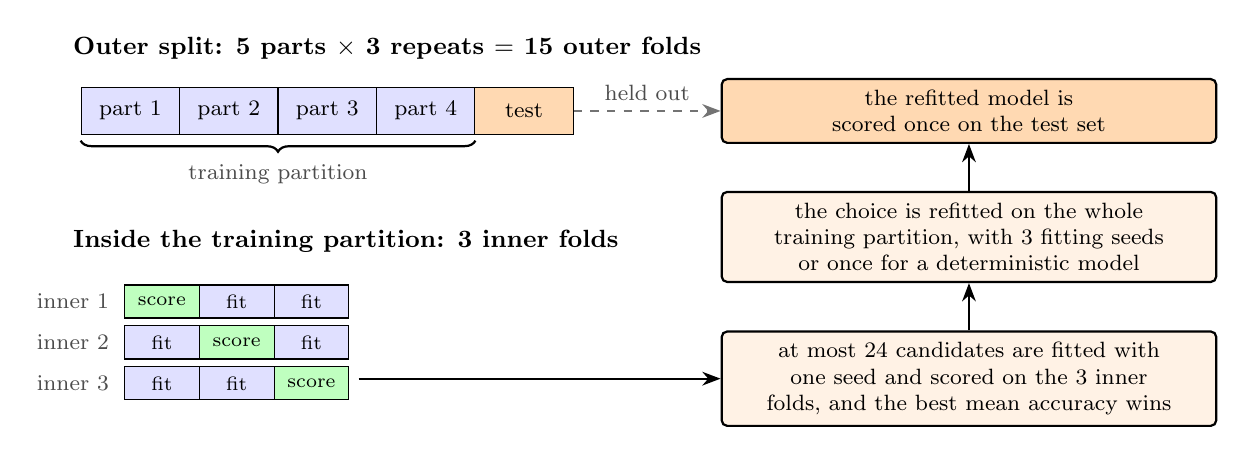
\begin{tikzpicture}[
    >=Stealth,
    part/.style={draw, minimum width=1.25cm, minimum height=0.6cm, font=\footnotesize, inner sep=0pt},
    trainpart/.style={part, fill=blue!12},
    testpart/.style={part, fill=orange!30},
    inner/.style={draw, minimum width=0.95cm, minimum height=0.42cm, font=\scriptsize, inner sep=0pt},
    fitpart/.style={inner, fill=blue!12},
    valpart/.style={inner, fill=green!25},
    box/.style={draw, rounded corners=2pt, font=\footnotesize, align=center, thick, minimum height=0.7cm, inner sep=4pt},
    arr/.style={->, thick},
    lbl/.style={font=\footnotesize, text=black!70},
]
% ----- the outer split: five stratified parts, one of them the test set
\node[font=\small\bfseries, anchor=west] at (-0.2,1.15) {Outer split: 5 parts $\times$ 3 repeats $=$ 15 outer folds};
\foreach \i in {1,...,4} { \node[trainpart] (o\i) at (1.25*\i-0.6,0.35) {part \i}; }
\node[testpart] (o5) at (1.25*5-0.6,0.35) {test};
\draw[decorate, decoration={brace, mirror, amplitude=4pt}, thick] ([yshift=-2pt]o1.south west) -- ([yshift=-2pt]o4.south east)
      node[midway, below=5pt, lbl] {training partition};
% ----- the inner split of the training partition
\node[font=\small\bfseries, anchor=west] at (-0.2,-1.3) {Inside the training partition: 3 inner folds};
\foreach \r in {1,2,3} {
  \foreach \c in {1,2,3} {
    \ifnum\c=\r \node[valpart] at (0.95*\c+0.1,-1.55-0.52*\r) {score}; \else \node[fitpart] at (0.95*\c+0.1,-1.55-0.52*\r) {fit}; \fi
  }
  \node[lbl, anchor=east] at (0.5,-1.55-0.52*\r) {inner \r};
}
% ----- the choice, the refit and the one test score, stacked on the right
\node[box, fill=orange!30, text width=6.0cm] (score) at (11.3,0.35) {the refitted model is scored once on the test set};
\node[box, fill=orange!10, text width=6.0cm] (refit) at (11.3,-1.25) {the choice is refitted on the whole training partition, with 3 fitting seeds or once for a deterministic model};
\node[box, fill=orange!10, text width=6.0cm] (choose) at (11.3,-3.05) {at most 24 candidates are fitted with one seed and scored on the 3 inner folds, and the best mean accuracy wins};
\draw[arr] (3.55,-3.05) -- (choose.west);
\draw[arr] (choose) -- (refit);
\draw[arr] (refit) -- (score);
\draw[arr, dashed, black!55] (o5.east) -- (score.west) node[midway, above, lbl] {held out};
\end{tikzpicture}
\caption{\textbf{Nested cross-validation.} Each dataset is split into five parts that keep its class proportions, and the split is repeated three times with new shuffles. So every model is tested on the same 15 outer folds. In each outer fold, one part is the test set and the other four form the training partition. Every choice is made inside the training partition. It is split again into three inner folds, and each model fits at most 24 candidate configurations with one fitting seed and scores them on those folds. For a stochastic model, one whose fit depends on a random seed, the three best candidates are then rescored with all three fitting seeds. The chosen configuration is refitted on the whole training partition, with the three fitting seeds or once for a deterministic model. It is then scored once on the test set, which no choice ever sees.}
\label{fig:s-nested-cv}
\end{figure}


ArrowFlow additionally chooses the neighbor count and weighting of each view's nearest-neighbor readout inside every fit, outside this budget. Every preprocessing step is fitted on the rows of the partition it is given. The checkpoint and readout splits are drawn from rows the encoder has already seen.

\paragraph{Models.} ArrowFlow's grid has 16 candidates. It takes every combination of the hidden-layer widths $[128]$ and $[64,128]$, the initial learning rate $\eta\in\{0.1,0.2\}$, a scale of 1 or 2 on the encoded vocabulary size $e$, and an offset of $0$ or $-1$ on the degree $p$. An adaptive rule sets the base values of $e$ and $p$ and the augmentation switch from the training partition. ArrowFlow fixes $K=7$ views, the nearest-neighbor readout, the majority vote and the validation checkpoint with $\nu=0.1$. Its readout settings are chosen by cross-validation over the training rows. The hidden rankings of these rows come from a network fitted on those same rows, so the choice carries some optimism. The prototype readout, the ablation of ArrowFlow that predicts with the nearest output filter, ran with the same grid in a separate run on the same partitions of the benchmark datasets. Each comparison model fits an imputer. The support vector classifier, the multilayer perceptron and numeric nearest neighbors also standardize the features. The majority class gives the baseline.

\paragraph{Means and intervals.} Tables give the mean and standard deviation (SD) over the 15 outer folds after averaging fitting seeds within each fold. The SD describes how widely the results spread across the folds. It is not a measure of uncertainty. To compare two models on one dataset, we form a paired accuracy difference on each of the $15$ outer folds, after averaging the fitting seeds within the fold. We call such a paired comparison a contrast. When we count the datasets on which one model is ahead, we use the sign of the unrounded difference. So a difference printed as $\pm0.00$ can count either way.

The 15 splits share training data, so the differences of a contrast are correlated. A standard $t$ interval, the textbook interval for a mean, would treat them as independent. The corrected resampled-$t$ interval \citep{nadeau2003inference,bouckaert2004evaluating} widens it to allow for the correlation. Like the textbook interval, it is the mean difference plus or minus a $t$ quantile times the square root of a scaled sample variance. In this interval, the sample variance of the $15$ differences is multiplied by $1/15+0.25$, where $0.25$ is the test-to-training ratio of the protocol. The $t$ quantile has $14$ degrees of freedom. A contrast over a subset of $n$ outer folds uses $1/n+0.25$ and $n-1$ degrees of freedom. The ratio is the size of a test fold divided by the size of its outer training partition. The textbook interval would multiply the variance by $1/15$ alone, so the added $0.25$ is what widens it. The corrected statistic also gives each contrast its $p$ value. It is an approximation, so its $p$ values are approximate.

\paragraph{The Holm adjustment.} When many contrasts are tested, some can look significant by chance alone. The Holm adjustment \citep{holm1979simple} guards against this. The comparisons that share one Holm adjustment form a family. The adjustment sorts the $p$ values of a family from smallest to largest. The smallest must fall below $0.05$ divided by the number of contrasts in the family, the next below $0.05$ divided by one less, and so on. The check stops at the first $p$ value that misses its threshold, and only the contrasts before it are significant. Equivalently, a contrast is significant when its Holm-adjusted $p$ value is below $0.05$. The adjustment bounds the probability of any false rejection in its family, that is, of calling a contrast significant when there is no true difference. It does so only as far as the $p$ values of the corrected statistic are valid.

Each family of contrasts is declared in its own protocol and adjusted only within itself. The families include the fourteen benchmark training contrasts, the fourteen contrasts of the sorting control and the two families of ten contrasts on the further datasets. The seven contrasts of ArrowFlow with the prototype readout and the fourteen contrasts fixed in the benchmark protocol form two more families. The stratum test on the further datasets compares the four marked datasets with the other six (Section~\ref{sec:training-controls}). It is an exact permutation test, and its $p$ value is the share of the 210 splits of the ten datasets into four and six whose difference of mean training effects is at least the observed one. In other words, the $p$ value is the chance that four datasets picked at random from the ten would show a difference at least as large. The matched protocol's own family of fourteen contrasts is reported for completeness with the matched study, and no claim rests on it.

\paragraph{When the families were fixed.} A family is registered when a run protocol fixed it before its comparisons were scored. Analyses defined afterwards are called post hoc. Every protocol of a family that scores outer folds is a file frozen with a recorded hash (Section~\ref{supp:protocols}), and none was deposited with an external registry. The hash is a fingerprint of the file's contents, so any later change to the file would show. The family of fourteen training contrasts on the benchmark datasets was registered after the outer results of ArrowFlow and of the prototype readout on these datasets were known. The two families of ten on the further datasets and their stratum test were registered before those runs. The prototype-readout protocol fixed its family of fourteen prototype-readout contrasts before its outer folds were scored. No registered adjustment spans two families. So Holm controls errors within one family only. Across the many families of this paper a few false positives are expected, and a result with an adjusted $p$ value near $0.05$ is fragile. One Holm adjustment over all 34 training contrasts, defined after every result was known, is reported as a post hoc sensitivity analysis. It shows which training results survive this stricter correction. Every other comparison of the training controls is descriptive. The controlled experiments of Sections~\ref{sec:motion-controls} and~\ref{sec:controlled} and the two studies of the encoder network declare their own families. Table~\ref{tab:study-map} lists those of the controlled experiments, and Section~\ref{supp:learned} gives those of the encoder network.

\section{Complete Results}\label{supp:results}

This section holds the details and the complete tables behind Section~\ref{sec:experiments} of the main text. Most subsections are headed with the part of Section~\ref{sec:experiments} they support. Table~\ref{tab:study-map} maps what each comparison asks. The subsections first cover the selection of the ten further datasets and then the benchmark and the training controls on all seventeen datasets. They go on to the sorting control, the prototype-readout contrasts with the matched study, and the eight controlled experiments of Sections~\ref{sec:motion-controls} and~\ref{sec:controlled}.

Every network with two hidden layers in this supplement used an earlier version of the relay of Section~\ref{sec:training}, one that did not carry the sign of the vote. We call it the earlier relay. The two corrected arms of the depth study in Section~\ref{supp:controlled} are the only exceptions.

Several reduced systems appear under distinct names:
\begin{itemize}[leftmargin=2em,topsep=2pt,itemsep=1pt]
\item The untrained ArrowFlow and tuned input footrule kNN are the training controls. Each chooses its own configuration on inner folds.
\item The untrained networks and footrule kNN on the same encoded inputs are variants of the component ablation, at ArrowFlow's own configuration. The frozen arm of the motion controls predicts exactly as those untrained networks.
\item Fixed-configuration input footrule kNN is the single-view classifier of the matched study.
\item The seven-view footrule kNN control is the reference of the prototype-readout contrasts.
\end{itemize}

The component ablation and the aggregation rules at the readout and the update are in Section~\ref{supp:ablations}. A script renders every table from the run files listed in Section~\ref{supp:reproducibility}. The script checks that every cell of a main-text table equals the cell of the same row and column in the corresponding complete table here. Error rates are in percent and differences in percentage points (pp). A standard deviation (SD) in parentheses measures the spread over the 15 outer folds, the test sets of the nested cross-validation. The fitting seeds are averaged within each fold first.

% Study map of Section 7, printed at the start of Section S3. Hand-written: it names comparisons, not numbers.
\begin{table}[!htbp]
\caption{\textbf{Study map.} What each comparison of Section~\ref{sec:experiments} asks, what ArrowFlow is set against, which settings the two sides share, and which analysis family carries it. A registered family is fixed in a frozen run protocol; every other comparison is descriptive. Contrasts from different rows are not comparable effect sizes.}
\label{tab:study-map}
\centering
\scriptsize
\begin{tabular}{@{}p{0.155\textwidth} p{0.185\textwidth} p{0.235\textwidth} p{0.285\textwidth}@{}}
\toprule
Question & Reference & Shared settings & Analysis \\
\midrule
Does ArrowFlow reach tuned classical accuracy? (Section~\ref{sec:main-benchmark}) &
five tuned classical models and the majority class &
folds only; every model chooses its own configuration on the inner folds &
descriptive, with a post hoc Friedman and Nemenyi comparison \\
\addlinespace
What does the learning rule add? (Section~\ref{sec:training-controls}) &
the untrained ArrowFlow; tuned input footrule kNN &
folds, fitting seeds and readout selection; each control chooses its own configuration &
three registered families, Holm within each; one post hoc Holm over all of them and post hoc signed-rank tests across the datasets \\
\addlinespace
Does sorting the projected scores help? (Section~\ref{supp:sorting}) &
numeric kNN on the projected scores &
folds and encoder candidates; each side chooses its own encoder settings &
one registered family, Holm within it \\
\addlinespace
What does each component contribute? (Section~\ref{sec:components}) &
variants of ArrowFlow &
folds, fitting seeds and ArrowFlow's own selected configuration &
descriptive \\
\addlinespace
Does the returned signal carry information? (Section~\ref{sec:motion-controls}) &
frozen filters, which predict exactly as the untrained networks of the component ablation; permuted alignment; random directions &
encoder, readout, folds, fitting seeds and configuration &
Holm within each arm over the seventeen datasets; each scramble against frozen filters post hoc \\
\addlinespace
What does training do, and where does it stop? (Section~\ref{sec:controlled}) &
mechanism and diagnostics; depth, with the earlier and the corrected relay; aggregation; neighbor baselines; the untrained and input rankings under a fixed Kendall-kernel readout &
folds and, in the fitted studies, one configuration per fold &
Holm within each family, or descriptive where stated \\
\bottomrule
\end{tabular}
\end{table}


\FloatBarrier
\subsection{Details for Section~\ref*{sec:protocol}: Dataset Selection}\label{supp:selection}

This subsection records how the ten further datasets of Section~\ref{sec:protocol} were chosen and pinned, each to one exact version of its OpenML file. Their strata and analysis were frozen in two batch protocols before any outer fold was scored, and every eligible dataset was run and is reported. The strata, defined below, split these datasets into two groups for a test of where training helps most.

\paragraph{Eligibility.} A dataset had to come from a fixed pool and pass a list of rules. The pool, or sampling frame, was the union of OpenML-CC18 and OpenML100 \citep{bischl2021openml} with the OpenML copies of datasets of the University of California, Irvine (UCI) repository. A dataset was eligible with 300 to 3,000 rows, 4 to 60 features, 2 to 10 classes, a smallest class of at least 30 rows, missing values in at most 5\% of cells and exact duplicate rows in at most 5\% of rows. It also had to be all numeric, free of target leakage, neither a time series nor an artificial generator outside OpenML-CC18, licensed for research use and neither a benchmark dataset nor a copy of one. Target leakage means that a feature gives away the class label.

Some rules needed interpretation. One OpenML copy of each source was considered. A placeholder zero is a zero recorded where a value was not measured. Placeholder zeros were not counted as missing. Of the 763 zero cells of diabetes, 652, $10.6\%$ of its cells, are placeholder zeros in five measurement columns and 111 are zero pregnancy counts. These interpretations of the rules were settled during selection, before any model was fitted. The rules narrowed the candidates in stages. Of 767 active OpenML datasets in the size and class range, 363 passed the metadata filter, 46 were in the frame and 10 passed every rule.

\paragraph{Published evidence and strata.} We split the further datasets into two strata by how far nearest neighbors trailed the best tuned models in published results. The counted sources are OpenML evaluations with at least ten runs of a nearest-neighbor classifier (kNN) and the accuracy table of \citet{fernandezdelgado2014hundreds}. When a task had fewer than ten standardized kNN runs, range-normalized kNN runs were pooled, and this pooling gives mfeat-zernike its counted source. A dataset was marked when a counted source put tuned kNN at least 5.0 pp behind the best tuned random forest, support vector machine or gradient boosting and no counted source covering all three put it closer (Table~\ref{tab:s-newdata-evidence}). The six remaining datasets form the other stratum.

The hepatitis C virus (HCV) data have no OpenML evaluations and no benchmark-table entry. The HCV target is the baseline histological staging of the OpenML copy (data ID 46850, version 2), with class counts 336, 332, 355 and 362. Its 28 features include 10 laboratory measurements taken during and after treatment, so the task is a retrospective classification of the recorded stage rather than a prediction from information available at baseline. Histological staging reads the stage of the disease from a tissue sample.

Table~\ref{tab:s-newdata-evidence} also gives each dataset's gap, the number of pp by which the best tuned kNN trails the best tuned random forest, support vector machine or gradient boosting. The Gap column, which the correlation of Section~\ref{supp:training} uses, averages every available source, including OpenML values from fewer than ten kNN runs. Counting only the sources of the stratum rule, and the single uncounted source of climate-model-simulation-crashes, which has no counted one, leaves the ranks of the nine gaps unchanged. That correlation is a Spearman correlation, which uses only ranks.

% Rendered by render_tables.py from run files; do not edit by hand.
\begin{table}[!htbp]
\caption{\textbf{Pins and published evidence of the further datasets.} For every dataset: its OpenML data identifier and version, the rows, features and classes and the size of the smallest class as prepared, its stratum and the first twelve hexadecimal digits of the content hash recorded at preparation. The gap is the best tuned random forest, support vector machine or gradient boosting minus the best tuned kNN, in percentage points. Its sources are the OpenML evaluations of the dataset's task \citep{vanschoren2014openml} and the accuracy table of \citet{fernandezdelgado2014hundreds} (2014 table); the Gap column averages them. $^\ddagger$: fewer than ten kNN runs, a source the stratum rule did not count. HCV: hepatitis C virus data of Egyptian patients, with no OpenML evaluations or benchmark-table entry. The protocols pin every value together with the checksums of the OpenML files.}
\label{tab:s-newdata-evidence}
\centering
\scriptsize
\setlength{\tabcolsep}{3pt}
\resizebox{\ifdim\width>\linewidth\linewidth\else\width\fi}{!}{%
\begin{tabular}{llrrrrlrll}
\toprule
Dataset & OpenML ID & Rows & Features & Classes & \begin{tabular}[b]{@{}r@{}}Smallest\\class\end{tabular} & Stratum & Gap (pp) & Sources (pp) & Hash \\
\midrule
balance-scale & 11 (v1) & 625 & 4 & 3 & 49 & marked & 9.50 & OpenML task 11: 9.9; 2014 table: 9.1 & \texttt{498096feb1f6} \\
mfeat-zernike & 22 (v1) & 2,000 & 47 & 10 & 200 & marked & 8.70 & OpenML task 22: 8.7 & \texttt{5160d61c6e08} \\
ionosphere & 59 (v1) & 351 & 34 & 2 & 126 & marked & 7.90 & OpenML task 57: 6.3; 2014 table: 9.5 & \texttt{dda052743b36} \\
vertebra-column & 1523 (v1) & 310 & 6 & 3 & 60 & marked & 7.25 & OpenML task 9939: 7.4$^\ddagger$; 2014 table: 7.1 & \texttt{3770457475ec} \\
diabetes & 37 (v1) & 768 & 8 & 2 & 268 & other & 1.95 & OpenML task 37: 3.5; 2014 table: 0.4 & \texttt{26f50df67316} \\
banknote-authentication & 1462 (v1) & 1,372 & 4 & 2 & 610 & other & 0.10 & OpenML task 10093: 0.1 & \texttt{50f2701a1e12} \\
qsar-biodeg & 1494 (v1) & 1,055 & 41 & 2 & 356 & other & 2.30 & OpenML task 9957: 2.3 & \texttt{d98d99ce1cb5} \\
steel-plates-fault & 40982 (v3) & 1,941 & 27 & 7 & 55 & other & 6.00 & OpenML task 146817: 7.4$^\ddagger$; 2014 table: 4.6 & \texttt{f4408a76aa4a} \\
climate-model-simulation-crashes & 40994 (v4) & 540 & 18 & 2 & 46 & other & 4.10 & OpenML task 146819: 4.1$^\ddagger$ & \texttt{6c76b66184fc} \\
HCV & 46850 (v2) & 1,385 & 28 & 4 & 332 & other & -- & none & \texttt{284048565b76} \\
\bottomrule
\end{tabular}
}
\end{table}


\FloatBarrier
\subsection{Details for Section~\ref*{sec:main-benchmark}: Main Benchmark}\label{supp:benchmark}

This subsection gives the complete benchmark and shows where ArrowFlow stands among the tuned models. Tables~\ref{tab:s-errors}, \ref{tab:s-balanced} and~\ref{tab:s-macro-f1} give the error, balanced accuracy and macro-F1 of the models of Table~\ref{tab:main} on the seventeen datasets. Balanced accuracy averages the recall of each class, the share of its rows that the model gets right. Macro-F1 averages the F1 score of each class in the same way. Both give a rare class the same weight as a common one.

On the benchmark datasets, the results of ArrowFlow and the classical models come from ArrowFlow's run on the benchmark's outer partitions. On the further datasets they come from the two batch runs. The combined analysis, \texttt{holistic benchmark}, fits no model and checks every value against the verified runs. The classical models are a support vector classifier (SVC) with a radial basis function (RBF) kernel, a random forest, a multilayer perceptron (MLP), numeric kNN and gradient boosting. The multilayer perceptron reached its iteration cap before convergence on 331 of its 765 outer fits, 77 of the 315 on the benchmark datasets and 254 of the 450 on the further datasets, and on every fit of vertebra-column and steel-plates-fault. The cap is the tuned \texttt{max\_iter} of Table~\ref{tab:s-grids}, which counts passes over the training data for this solver. So the warning records an exhausted budget of passes. It does not mark a failed fit.

% Rendered by render_tables.py from run files; do not edit by hand.
\begin{table}[!htbp]
\caption{\textbf{Complete error of the models of Table~\ref{tab:main}.} Mean outer-fold error in percent (outer-fold SD) [mean within-fold SD across the three fitting seeds] on the seventeen datasets. Deterministic models have one fitting seed per fold and no seed SD. SVC: support vector classifier; MLP: multilayer perceptron; kNN: nearest-neighbor classifier; HCV: hepatitis C virus.}
\label{tab:s-errors}
\centering
\scriptsize
\setlength{\tabcolsep}{3pt}
\begin{tabular}{lrrrr}
\toprule
Dataset & ArrowFlow & SVC (RBF) & Random forest & MLP \\
\midrule
\multicolumn{5}{l}{\emph{Benchmark datasets}} \\
Iris & 5.0 (3.5) [1.4] & 4.0 (3.4) & 5.3 (4.3) [0.4] & 4.1 (3.7) [0.4] \\
Wine & 3.2 (2.9) [1.6] & 1.5 (2.3) & 1.8 (1.6) [0.3] & 1.9 (2.2) [0.5] \\
Breast cancer & 2.7 (1.1) [0.7] & 2.3 (1.5) & 4.3 (1.5) [0.5] & 2.9 (1.5) [0.4] \\
Wine quality & 27.7 (2.1) [1.1] & 33.1 (3.4) & 27.2 (2.3) [0.7] & 32.3 (2.6) [1.4] \\
Vehicle & 19.9 (1.5) [1.6] & 16.5 (2.0) & 25.7 (2.3) [1.3] & 17.2 (2.0) [1.4] \\
Segment & 2.6 (0.7) [0.2] & 3.3 (0.9) & 1.9 (0.7) [0.2] & 2.8 (0.9) [0.4] \\
Digits & 2.8 (0.9) [0.4] & 1.8 (0.6) & 2.4 (0.7) [0.3] & 2.3 (0.8) [0.3] \\
\midrule
\multicolumn{5}{l}{\emph{Further datasets}} \\
balance-scale & 6.0 (1.3) [1.1] & 2.1 (1.8) & 13.8 (2.1) [0.7] & 2.2 (1.1) [0.3] \\
mfeat-zernike & 19.3 (1.0) [0.9] & 17.1 (1.6) & 22.3 (2.0) [0.7] & 18.9 (1.2) [0.6] \\
ionosphere & 11.2 (3.4) [1.9] & 5.9 (2.7) & 7.0 (2.5) [0.4] & 8.0 (2.6) [1.1] \\
vertebra-column & 16.9 (3.6) [1.9] & 14.0 (5.2) & 15.8 (3.2) [0.8] & 15.4 (4.4) [1.1] \\
diabetes & 24.0 (2.5) [1.3] & 22.7 (2.9) & 23.9 (2.6) [0.8] & 23.5 (1.5) [1.3] \\
banknote-authentication & 0.2 (0.5) [0.1] & 0.0 (0.1) & 0.9 (0.7) [0.1] & 0.0 (0.0) [0.0] \\
qsar-biodeg & 12.6 (1.8) [0.8] & 12.2 (3.1) & 13.0 (2.1) [0.5] & 12.0 (2.9) [0.7] \\
steel-plates-fault & 24.8 (1.5) [1.0] & 23.9 (2.1) & 21.2 (1.6) [0.6] & 24.2 (1.7) [0.9] \\
climate-model-simulation-crashes & 8.3 (0.6) [0.3] & 5.4 (2.2) & 6.4 (1.1) [0.4] & 5.6 (1.7) [0.8] \\
HCV & 75.6 (1.7) [2.3] & 75.5 (2.0) & 75.9 (1.6) [1.6] & 75.0 (1.8) [2.2] \\
\bottomrule
\end{tabular}
\par\medskip
\begin{tabular}{lrrr}
\toprule
Dataset & Numeric kNN & \begin{tabular}[b]{@{}r@{}}Gradient\\boosting\end{tabular} & \begin{tabular}[b]{@{}r@{}}Majority\\class\end{tabular} \\
\midrule
\multicolumn{4}{l}{\emph{Benchmark datasets}} \\
Iris & 4.7 (3.3) & 5.6 (3.5) [0.0] & 66.7 (0.0) \\
Wine & 3.4 (3.4) & 2.6 (2.5) [0.0] & 60.1 (1.6) \\
Breast cancer & 3.5 (1.5) & 3.9 (1.6) [0.1] & 37.3 (0.4) \\
Wine quality & 28.8 (2.2) & 30.7 (2.1) [0.1] & 53.5 (0.1) \\
Vehicle & 29.3 (2.6) & 24.3 (2.2) [0.3] & 74.2 (0.3) \\
Segment & 3.4 (1.1) & 2.1 (0.6) [0.1] & 85.7 (0.0) \\
Digits & 2.1 (0.7) & 3.3 (0.9) [0.1] & 89.9 (0.2) \\
\midrule
\multicolumn{4}{l}{\emph{Further datasets}} \\
balance-scale & 10.2 (1.5) & 8.4 (0.8) [0.0] & 54.2 (0.3) \\
mfeat-zernike & 19.6 (1.7) & 22.4 (1.8) [0.2] & 90.0 (0.0) \\
ionosphere & 10.2 (3.5) & 6.6 (2.1) [0.0] & 35.9 (0.4) \\
vertebra-column & 19.8 (4.0) & 17.8 (4.3) [0.0] & 51.6 (0.0) \\
diabetes & 24.5 (2.7) & 24.0 (3.2) [0.0] & 34.9 (0.2) \\
banknote-authentication & 0.3 (0.5) & 0.3 (0.3) [0.0] & 44.5 (0.1) \\
qsar-biodeg & 13.7 (2.7) & 13.2 (2.5) [0.1] & 33.7 (0.2) \\
steel-plates-fault & 25.5 (1.4) & 21.0 (1.8) [0.4] & 65.3 (0.1) \\
climate-model-simulation-crashes & 6.8 (1.1) & 5.9 (1.4) [0.1] & 8.5 (0.4) \\
HCV & 74.1 (2.6) & 76.9 (2.4) [0.1] & 73.9 (0.2) \\
\bottomrule
\end{tabular}
\end{table}

% Rendered by render_tables.py from run files; do not edit by hand.
\begin{table}[!htbp]
\caption{\textbf{Balanced accuracy of the models of Table~\ref{tab:main}.} Mean outer-fold balanced accuracy in percent, the unweighted mean of the per-class recalls, with the outer-fold SD in parentheses. Accuracy is the metric of every registered analysis, so this table is descriptive.}
\label{tab:s-balanced}
\centering
\scriptsize
\setlength{\tabcolsep}{3pt}
\begin{tabular}{lrrrr}
\toprule
Dataset & ArrowFlow & SVC (RBF) & Random forest & MLP \\
\midrule
\multicolumn{5}{l}{\emph{Benchmark datasets}} \\
Iris & 95.0 (3.5) & 96.0 (3.4) & 94.7 (4.3) & 95.9 (3.7) \\
Wine & 97.3 (2.5) & 98.7 (2.0) & 98.5 (1.4) & 98.3 (2.1) \\
Breast cancer & 96.9 (1.4) & 97.2 (2.0) & 95.2 (1.8) & 96.7 (1.9) \\
Wine quality & 68.2 (2.8) & 61.2 (3.7) & 68.3 (2.4) & 65.3 (3.5) \\
Vehicle & 80.3 (1.6) & 83.7 (2.1) & 74.6 (2.2) & 83.0 (2.0) \\
Segment & 97.4 (0.7) & 96.7 (0.9) & 98.1 (0.7) & 97.2 (0.9) \\
Digits & 97.2 (0.9) & 98.2 (0.6) & 97.6 (0.7) & 97.7 (0.8) \\
\midrule
\multicolumn{5}{l}{\emph{Further datasets}} \\
balance-scale & 82.5 (4.8) & 97.2 (3.4) & 62.4 (1.5) & 96.5 (2.9) \\
mfeat-zernike & 80.7 (1.0) & 82.9 (1.6) & 77.7 (2.0) & 81.1 (1.2) \\
ionosphere & 85.5 (4.5) & 93.2 (2.9) & 91.8 (3.0) & 89.9 (3.3) \\
vertebra-column & 79.9 (3.7) & 82.3 (5.8) & 79.3 (3.5) & 80.5 (4.9) \\
diabetes & 72.1 (2.7) & 71.7 (3.2) & 71.9 (2.6) & 72.4 (1.9) \\
banknote-authentication & 99.8 (0.4) & 100.0 (0.1) & 99.1 (0.7) & 100.0 (0.0) \\
qsar-biodeg & 86.2 (1.8) & 86.0 (3.5) & 84.4 (2.6) & 86.1 (3.3) \\
steel-plates-fault & 77.7 (2.7) & 76.8 (3.6) & 79.3 (2.5) & 77.6 (2.8) \\
climate-model-simulation-crashes & 51.2 (2.2) & 76.1 (7.1) & 65.1 (5.7) & 76.0 (7.8) \\
HCV & 24.5 (1.7) & 24.0 (1.8) & 23.8 (1.6) & 24.9 (1.7) \\
\bottomrule
\end{tabular}
\par\medskip
\begin{tabular}{lrrr}
\toprule
Dataset & Numeric kNN & \begin{tabular}[b]{@{}r@{}}Gradient\\boosting\end{tabular} & \begin{tabular}[b]{@{}r@{}}Majority\\class\end{tabular} \\
\midrule
\multicolumn{4}{l}{\emph{Benchmark datasets}} \\
Iris & 95.3 (3.3) & 94.4 (3.5) & 33.3 (0.0) \\
Wine & 97.2 (2.9) & 97.8 (2.2) & 33.3 (0.0) \\
Breast cancer & 95.9 (1.7) & 95.5 (1.9) & 50.0 (0.0) \\
Wine quality & 67.9 (2.6) & 65.2 (2.8) & 33.3 (0.0) \\
Vehicle & 70.9 (2.6) & 75.9 (2.3) & 25.0 (0.0) \\
Segment & 96.6 (1.1) & 97.9 (0.6) & 14.3 (0.0) \\
Digits & 97.9 (0.7) & 96.7 (0.9) & 10.0 (0.0) \\
\midrule
\multicolumn{4}{l}{\emph{Further datasets}} \\
balance-scale & 64.9 (1.1) & 66.2 (0.6) & 33.3 (0.0) \\
mfeat-zernike & 80.3 (1.7) & 77.6 (1.8) & 10.0 (0.0) \\
ionosphere & 86.7 (4.8) & 91.8 (2.8) & 50.0 (0.0) \\
vertebra-column & 76.2 (4.4) & 76.0 (6.0) & 33.3 (0.0) \\
diabetes & 69.8 (2.6) & 71.1 (3.5) & 50.0 (0.0) \\
banknote-authentication & 99.7 (0.4) & 99.7 (0.3) & 50.0 (0.0) \\
qsar-biodeg & 85.2 (3.1) & 84.3 (2.9) & 50.0 (0.0) \\
steel-plates-fault & 77.2 (2.7) & 79.3 (3.1) & 14.3 (0.0) \\
climate-model-simulation-crashes & 63.0 (6.2) & 70.0 (7.6) & 50.0 (0.0) \\
HCV & 25.8 (2.6) & 22.9 (2.4) & 25.0 (0.0) \\
\bottomrule
\end{tabular}
\end{table}

% Rendered by render_tables.py from run files; do not edit by hand.
\begin{table}[!htbp]
\caption{\textbf{Macro-F1 of the models of Table~\ref{tab:main}.} Mean outer-fold macro-F1 in percent, the unweighted mean of the per-class F1 scores, where a class that is never predicted scores 0, with the outer-fold SD in parentheses. Descriptive.}
\label{tab:s-macro-f1}
\centering
\scriptsize
\setlength{\tabcolsep}{3pt}
\begin{tabular}{lrrrr}
\toprule
Dataset & ArrowFlow & SVC (RBF) & Random forest & MLP \\
\midrule
\multicolumn{5}{l}{\emph{Benchmark datasets}} \\
Iris & 94.9 (3.5) & 96.0 (3.4) & 94.7 (4.3) & 95.8 (3.7) \\
Wine & 96.9 (2.9) & 98.5 (2.3) & 98.2 (1.6) & 98.1 (2.3) \\
Breast cancer & 97.1 (1.2) & 97.5 (1.7) & 95.4 (1.6) & 96.9 (1.7) \\
Wine quality & 69.3 (2.5) & 62.8 (4.1) & 69.7 (2.2) & 65.5 (3.0) \\
Vehicle & 79.9 (1.6) & 83.5 (2.0) & 73.6 (2.6) & 82.9 (2.0) \\
Segment & 97.4 (0.7) & 96.7 (0.9) & 98.1 (0.7) & 97.2 (0.9) \\
Digits & 97.2 (0.9) & 98.2 (0.6) & 97.6 (0.7) & 97.7 (0.8) \\
\midrule
\multicolumn{5}{l}{\emph{Further datasets}} \\
balance-scale & 84.2 (4.5) & 95.3 (4.1) & 60.2 (1.3) & 95.1 (2.5) \\
mfeat-zernike & 80.3 (1.2) & 82.6 (1.6) & 77.4 (2.1) & 81.1 (1.3) \\
ionosphere & 87.0 (4.1) & 93.5 (2.9) & 92.3 (2.7) & 91.0 (3.0) \\
vertebra-column & 79.4 (3.8) & 82.3 (5.9) & 79.5 (3.5) & 80.4 (5.1) \\
diabetes & 72.7 (2.8) & 72.9 (3.5) & 72.6 (2.7) & 73.0 (1.8) \\
banknote-authentication & 99.8 (0.5) & 100.0 (0.1) & 99.1 (0.7) & 100.0 (0.0) \\
qsar-biodeg & 86.0 (1.9) & 86.3 (3.4) & 85.1 (2.4) & 86.4 (3.3) \\
steel-plates-fault & 76.7 (2.6) & 77.6 (2.5) & 80.6 (2.2) & 78.0 (2.3) \\
climate-model-simulation-crashes & 49.8 (3.4) & 80.0 (7.6) & 70.1 (6.9) & 79.0 (7.6) \\
HCV & 24.1 (1.6) & 19.8 (6.2) & 23.3 (1.4) & 24.9 (1.7) \\
\bottomrule
\end{tabular}
\par\medskip
\begin{tabular}{lrrr}
\toprule
Dataset & Numeric kNN & \begin{tabular}[b]{@{}r@{}}Gradient\\boosting\end{tabular} & \begin{tabular}[b]{@{}r@{}}Majority\\class\end{tabular} \\
\midrule
\multicolumn{4}{l}{\emph{Benchmark datasets}} \\
Iris & 95.3 (3.3) & 94.4 (3.5) & 16.7 (0.0) \\
Wine & 96.7 (3.3) & 97.5 (2.4) & 19.0 (0.5) \\
Breast cancer & 96.3 (1.7) & 95.8 (1.7) & 38.6 (0.2) \\
Wine quality & 68.7 (2.5) & 66.3 (2.6) & 21.2 (0.0) \\
Vehicle & 69.7 (2.7) & 75.5 (2.5) & 10.2 (0.1) \\
Segment & 96.6 (1.1) & 97.9 (0.6) & 3.6 (0.0) \\
Digits & 97.9 (0.7) & 96.7 (0.9) & 1.8 (0.0) \\
\midrule
\multicolumn{4}{l}{\emph{Further datasets}} \\
balance-scale & 62.3 (1.0) & 63.6 (0.6) & 20.9 (0.1) \\
mfeat-zernike & 80.1 (1.8) & 77.8 (2.0) & 1.8 (0.0) \\
ionosphere & 88.2 (4.4) & 92.6 (2.4) & 39.1 (0.1) \\
vertebra-column & 76.3 (4.4) & 76.0 (6.2) & 21.7 (0.0) \\
diabetes & 70.9 (2.9) & 71.9 (3.8) & 39.4 (0.1) \\
banknote-authentication & 99.7 (0.5) & 99.7 (0.3) & 35.7 (0.0) \\
qsar-biodeg & 84.8 (2.9) & 84.9 (2.8) & 39.9 (0.1) \\
steel-plates-fault & 76.0 (2.0) & 81.0 (2.5) & 7.4 (0.0) \\
climate-model-simulation-crashes & 67.5 (8.2) & 74.8 (8.1) & 47.8 (0.1) \\
HCV & 25.5 (2.5) & 22.5 (2.4) & 10.4 (0.1) \\
\bottomrule
\end{tabular}
\end{table}


The next three tables show which configurations the inner folds chose. Table~\ref{tab:s-selected} lists the configurations that the prototype readout chose on the inner folds of the benchmark datasets. Tables~\ref{tab:s-knn-selected} and~\ref{tab:s-knn-selected-further} list those that ArrowFlow chose on the benchmark and the further datasets, by the inner-fold accuracy of its own readout.

% Rendered by render_tables.py from run files; do not edit by hand.
\begin{table}[!htbp]
\caption{\textbf{Configurations of the prototype readout chosen on the inner folds.} For every dataset, the configurations selected across the 15 outer folds of the nested benchmark from its 16 candidates. Each row gives the hidden widths, initial learning rate $\eta$, encoded vocabulary size $e$ and polynomial degree $p$ as resolved from the training partition, and the augmentation switch (resolved by the adaptive rule from the training partition). The remaining columns give the number of outer folds that chose the configuration and the mean inner-fold selection accuracy of those folds in percent. No outer-fold score enters the choice.}
\label{tab:s-selected}
\centering
\footnotesize
\setlength{\tabcolsep}{3pt}
\begin{tabular}{llrrrlrr}
\toprule
Dataset & Widths & $\eta$ & $e$ & $p$ & Augment & Folds & Inner acc. \\
\midrule
Iris & $[128]$ & 0.2 & 32 & 3 & off & 6 of 15 & 93.8 \\
 & $[128]$ & 0.2 & 16 & 3 & off & 2 of 15 & 94.7 \\
 & $[64,128]$ & 0.2 & 16 & 3 & off & 2 of 15 & 94.6 \\
 & $[128]$ & 0.1 & 32 & 3 & off & 1 of 15 & 92.2 \\
 & $[128]$ & 0.2 & 32 & 2 & off & 1 of 15 & 93.1 \\
 & $[64,128]$ & 0.1 & 16 & 3 & off & 1 of 15 & 92.5 \\
 & $[64,128]$ & 0.1 & 32 & 3 & off & 1 of 15 & 95.8 \\
 & $[64,128]$ & 0.2 & 32 & 3 & off & 1 of 15 & 94.4 \\
\midrule
Wine & $[64,128]$ & 0.2 & 32 & 2 & off & 4 of 15 & 96.2 \\
 & $[64,128]$ & 0.2 & 32 & 1 & off & 3 of 15 & 96.0 \\
 & $[128]$ & 0.2 & 32 & 2 & off & 2 of 15 & 97.2 \\
 & $[64,128]$ & 0.2 & 64 & 2 & off & 2 of 15 & 95.7 \\
 & $[128]$ & 0.1 & 64 & 1 & off & 1 of 15 & 95.6 \\
 & $[128]$ & 0.2 & 64 & 1 & off & 1 of 15 & 95.3 \\
 & $[128]$ & 0.2 & 64 & 2 & off & 1 of 15 & 96.0 \\
 & $[64,128]$ & 0.1 & 64 & 2 & off & 1 of 15 & 98.1 \\
\midrule
Breast cancer & $[128]$ & 0.1 & 32 & 1 & on & 4 of 15 & 97.1 \\
 & $[128]$ & 0.1 & 64 & 1 & on & 2 of 15 & 97.1 \\
 & $[128]$ & 0.2 & 64 & 1 & on & 2 of 15 & 97.2 \\
 & $[128]$ & 0.2 & 64 & 2 & on & 2 of 15 & 97.2 \\
 & $[64,128]$ & 0.1 & 32 & 1 & on & 2 of 15 & 97.2 \\
 & $[64,128]$ & 0.1 & 64 & 1 & on & 1 of 15 & 97.3 \\
 & $[64,128]$ & 0.2 & 64 & 1 & on & 1 of 15 & 96.9 \\
 & $[64,128]$ & 0.2 & 64 & 2 & on & 1 of 15 & 97.1 \\
\midrule
Wine quality & $[128]$ & 0.1 & 64 & 2 & on & 5 of 15 & 60.0 \\
 & $[128]$ & 0.1 & 32 & 2 & on & 4 of 15 & 59.7 \\
 & $[64,128]$ & 0.1 & 64 & 1 & on & 2 of 15 & 58.9 \\
 & $[128]$ & 0.1 & 64 & 1 & on & 1 of 15 & 59.9 \\
 & $[64,128]$ & 0.1 & 32 & 1 & on & 1 of 15 & 59.1 \\
 & $[64,128]$ & 0.1 & 64 & 2 & on & 1 of 15 & 59.0 \\
 & $[64,128]$ & 0.2 & 64 & 1 & on & 1 of 15 & 58.8 \\
\midrule
Vehicle & $[128]$ & 0.1 & 32 & 2 & on & 7 of 15 & 79.7 \\
 & $[128]$ & 0.1 & 64 & 2 & on & 5 of 15 & 80.5 \\
 & $[64,128]$ & 0.1 & 32 & 2 & on & 2 of 15 & 79.3 \\
 & $[64,128]$ & 0.1 & 64 & 2 & on & 1 of 15 & 79.0 \\
\midrule
Segment & $[128]$ & 0.2 & 64 & 2 & on & 10 of 15 & 94.7 \\
 & $[128]$ & 0.1 & 64 & 2 & on & 5 of 15 & 94.6 \\
\midrule
Digits & $[128]$ & 0.2 & 128 & 1 & off & 11 of 15 & 95.3 \\
 & $[128]$ & 0.2 & 64 & 1 & off & 4 of 15 & 94.8 \\
\bottomrule
\end{tabular}
\end{table}

% Rendered by render_tables.py from run files; do not edit by hand.
\begin{table}[!htbp]
\caption{\textbf{Configurations of ArrowFlow chosen on the inner folds, benchmark datasets.} For every benchmark dataset, the configurations selected across the 15 outer folds of the nested evaluation from its 16 candidates, read from the selection records of the ArrowFlow run. Each row gives the hidden widths, initial learning rate $\eta$, encoded vocabulary size $e$ and polynomial degree $p$ as resolved from the training partition, and the augmentation switch (resolved by the adaptive rule from the training partition). The remaining columns give the number of outer folds that chose the configuration and the mean inner-fold selection accuracy of those folds in percent, measured with ArrowFlow's own readout. No outer-fold score enters the choice.}
\label{tab:s-knn-selected}
\centering
\scriptsize
\setlength{\tabcolsep}{3pt}
\begin{tabular}{llrrrlrr}
\toprule
Dataset & Widths & $\eta$ & $e$ & $p$ & Augment & Folds & Inner acc. \\
\midrule
Iris & $[128]$ & 0.2 & 32 & 3 & off & 3 of 15 & 93.3 \\
 & $[64,128]$ & 0.1 & 16 & 3 & off & 3 of 15 & 94.1 \\
 & $[128]$ & 0.1 & 32 & 3 & off & 2 of 15 & 96.0 \\
 & $[128]$ & 0.2 & 16 & 3 & off & 2 of 15 & 94.6 \\
 & $[64,128]$ & 0.1 & 32 & 3 & off & 2 of 15 & 94.6 \\
 & $[128]$ & 0.1 & 16 & 3 & off & 1 of 15 & 96.1 \\
 & $[64,128]$ & 0.2 & 16 & 3 & off & 1 of 15 & 94.2 \\
 & $[64,128]$ & 0.2 & 32 & 3 & off & 1 of 15 & 93.6 \\
\midrule
Wine & $[64,128]$ & 0.2 & 32 & 1 & off & 7 of 15 & 96.6 \\
 & $[64,128]$ & 0.2 & 64 & 2 & off & 2 of 15 & 96.8 \\
 & $[128]$ & 0.1 & 64 & 2 & off & 1 of 15 & 95.8 \\
 & $[128]$ & 0.2 & 32 & 1 & off & 1 of 15 & 96.0 \\
 & $[128]$ & 0.2 & 64 & 1 & off & 1 of 15 & 97.0 \\
 & $[128]$ & 0.2 & 64 & 2 & off & 1 of 15 & 98.6 \\
 & $[64,128]$ & 0.1 & 32 & 1 & off & 1 of 15 & 97.4 \\
 & $[64,128]$ & 0.2 & 64 & 1 & off & 1 of 15 & 97.0 \\
\midrule
Breast cancer & $[128]$ & 0.1 & 32 & 1 & on & 4 of 15 & 97.4 \\
 & $[128]$ & 0.2 & 64 & 1 & on & 3 of 15 & 97.5 \\
 & $[64,128]$ & 0.2 & 32 & 1 & on & 3 of 15 & 97.6 \\
 & $[128]$ & 0.1 & 64 & 1 & on & 2 of 15 & 97.7 \\
 & $[128]$ & 0.2 & 64 & 2 & on & 2 of 15 & 97.2 \\
 & $[64,128]$ & 0.1 & 32 & 1 & on & 1 of 15 & 97.9 \\
\midrule
Wine quality & $[128]$ & 0.1 & 64 & 2 & on & 5 of 15 & 68.7 \\
 & $[128]$ & 0.1 & 32 & 1 & on & 2 of 15 & 69.4 \\
 & $[128]$ & 0.1 & 64 & 1 & on & 2 of 15 & 68.5 \\
 & $[128]$ & 0.2 & 32 & 1 & on & 2 of 15 & 69.7 \\
 & $[128]$ & 0.1 & 32 & 2 & on & 1 of 15 & 68.9 \\
 & $[128]$ & 0.2 & 32 & 2 & on & 1 of 15 & 68.4 \\
 & $[128]$ & 0.2 & 64 & 1 & on & 1 of 15 & 68.9 \\
 & $[128]$ & 0.2 & 64 & 2 & on & 1 of 15 & 68.8 \\
\midrule
Vehicle & $[128]$ & 0.1 & 32 & 2 & on & 5 of 15 & 80.4 \\
 & $[128]$ & 0.2 & 32 & 2 & on & 5 of 15 & 79.9 \\
 & $[64,128]$ & 0.1 & 32 & 2 & on & 3 of 15 & 80.1 \\
 & $[128]$ & 0.2 & 64 & 2 & on & 2 of 15 & 79.4 \\
\midrule
Segment & $[128]$ & 0.2 & 64 & 1 & on & 10 of 15 & 97.0 \\
 & $[128]$ & 0.1 & 64 & 1 & on & 4 of 15 & 96.8 \\
 & $[128]$ & 0.1 & 64 & 2 & on & 1 of 15 & 96.9 \\
\midrule
Digits & $[128]$ & 0.1 & 128 & 1 & off & 6 of 15 & 96.9 \\
 & $[128]$ & 0.1 & 64 & 1 & off & 4 of 15 & 96.8 \\
 & $[128]$ & 0.2 & 128 & 1 & off & 4 of 15 & 96.8 \\
 & $[128]$ & 0.2 & 64 & 1 & off & 1 of 15 & 96.9 \\
\bottomrule
\end{tabular}
\end{table}

% Rendered by render_tables.py from run files; do not edit by hand.
\begin{table}[!htbp]
\caption{\textbf{Configurations of ArrowFlow chosen on the inner folds, further datasets.} The same record as Table~\ref{tab:s-knn-selected}, read from the selection records of the two batch runs; no outer-fold score enters the choice. HCV: hepatitis C virus.}
\label{tab:s-knn-selected-further}
\centering
\scriptsize
\setlength{\tabcolsep}{3pt}
\renewcommand{\arraystretch}{0.85}
\begin{tabular}{llrrrlrr}
\toprule
Dataset & Widths & $\eta$ & $e$ & $p$ & Augment & Folds & Inner acc. \\
\midrule
balance-scale & $[128]$ & 0.2 & 32 & 2 & on & 9 of 15 & 93.0 \\
 & $[128]$ & 0.1 & 32 & 2 & on & 4 of 15 & 93.0 \\
 & $[128]$ & 0.1 & 32 & 3 & on & 1 of 15 & 92.9 \\
 & $[128]$ & 0.2 & 32 & 3 & on & 1 of 15 & 92.7 \\
\midrule
mfeat-zernike & $[128]$ & 0.1 & 128 & 1 & off & 11 of 15 & 81.9 \\
 & $[128]$ & 0.1 & 64 & 1 & off & 4 of 15 & 81.2 \\
\midrule
ionosphere & $[128]$ & 0.1 & 128 & 1 & off & 4 of 15 & 88.8 \\
 & $[128]$ & 0.2 & 64 & 1 & off & 4 of 15 & 89.7 \\
 & $[128]$ & 0.1 & 64 & 1 & off & 3 of 15 & 90.3 \\
 & $[64,128]$ & 0.1 & 128 & 1 & off & 2 of 15 & 88.8 \\
 & $[64,128]$ & 0.2 & 64 & 1 & off & 1 of 15 & 88.1 \\
 & $[64,128]$ & 0.2 & 128 & 1 & off & 1 of 15 & 89.9 \\
\midrule
vertebra-column & $[64,128]$ & 0.1 & 16 & 2 & on & 7 of 15 & 84.5 \\
 & $[128]$ & 0.1 & 16 & 3 & on & 2 of 15 & 84.3 \\
 & $[128]$ & 0.2 & 16 & 2 & on & 2 of 15 & 83.1 \\
 & $[64,128]$ & 0.1 & 32 & 2 & on & 2 of 15 & 84.1 \\
 & $[64,128]$ & 0.2 & 16 & 2 & on & 2 of 15 & 83.3 \\
\midrule
diabetes & $[128]$ & 0.2 & 16 & 2 & on & 4 of 15 & 75.2 \\
 & $[128]$ & 0.1 & 16 & 2 & on & 2 of 15 & 75.3 \\
 & $[128]$ & 0.1 & 32 & 2 & on & 2 of 15 & 75.6 \\
 & $[128]$ & 0.2 & 32 & 2 & on & 2 of 15 & 75.7 \\
 & $[64,128]$ & 0.2 & 16 & 2 & on & 2 of 15 & 75.9 \\
 & $[64,128]$ & 0.1 & 16 & 2 & on & 1 of 15 & 74.8 \\
 & $[64,128]$ & 0.1 & 32 & 2 & on & 1 of 15 & 75.2 \\
 & $[64,128]$ & 0.2 & 32 & 2 & on & 1 of 15 & 76.2 \\
\midrule
banknote-authentication & $[64,128]$ & 0.1 & 16 & 3 & on & 3 of 15 & 100.0 \\
 & $[64,128]$ & 0.2 & 32 & 2 & on & 3 of 15 & 99.9 \\
 & $[128]$ & 0.1 & 32 & 3 & on & 2 of 15 & 100.0 \\
 & $[128]$ & 0.2 & 16 & 2 & on & 2 of 15 & 99.9 \\
 & $[128]$ & 0.1 & 32 & 2 & on & 1 of 15 & 99.9 \\
 & $[128]$ & 0.2 & 16 & 3 & on & 1 of 15 & 100.0 \\
 & $[64,128]$ & 0.1 & 16 & 2 & on & 1 of 15 & 100.0 \\
 & $[64,128]$ & 0.1 & 32 & 3 & on & 1 of 15 & 99.9 \\
 & $[64,128]$ & 0.2 & 16 & 3 & on & 1 of 15 & 99.9 \\
\midrule
qsar-biodeg & $[128]$ & 0.1 & 128 & 1 & off & 6 of 15 & 86.4 \\
 & $[128]$ & 0.2 & 128 & 1 & off & 5 of 15 & 86.8 \\
 & $[128]$ & 0.1 & 64 & 1 & off & 2 of 15 & 87.5 \\
 & $[128]$ & 0.2 & 64 & 1 & off & 2 of 15 & 86.2 \\
\midrule
steel-plates-fault & $[128]$ & 0.1 & 64 & 2 & on & 7 of 15 & 73.8 \\
 & $[128]$ & 0.1 & 64 & 1 & on & 4 of 15 & 73.9 \\
 & $[128]$ & 0.1 & 32 & 1 & on & 1 of 15 & 73.5 \\
 & $[128]$ & 0.1 & 32 & 2 & on & 1 of 15 & 73.5 \\
 & $[128]$ & 0.2 & 32 & 1 & on & 1 of 15 & 73.0 \\
 & $[128]$ & 0.2 & 64 & 2 & on & 1 of 15 & 73.4 \\
\midrule
climate-model-simulation-crashes & $[128]$ & 0.1 & 64 & 2 & on & 7 of 15 & 92.2 \\
 & $[64,128]$ & 0.1 & 64 & 2 & on & 4 of 15 & 91.9 \\
 & $[128]$ & 0.2 & 64 & 2 & on & 2 of 15 & 91.8 \\
 & $[128]$ & 0.1 & 64 & 1 & on & 1 of 15 & 91.7 \\
 & $[64,128]$ & 0.1 & 32 & 2 & on & 1 of 15 & 92.1 \\
\midrule
HCV & $[64,128]$ & 0.1 & 32 & 1 & on & 3 of 15 & 26.0 \\
 & $[64,128]$ & 0.2 & 64 & 2 & on & 3 of 15 & 25.8 \\
 & $[64,128]$ & 0.1 & 64 & 1 & on & 2 of 15 & 26.2 \\
 & $[64,128]$ & 0.1 & 64 & 2 & on & 2 of 15 & 27.0 \\
 & $[128]$ & 0.1 & 32 & 1 & on & 1 of 15 & 25.9 \\
 & $[128]$ & 0.1 & 64 & 1 & on & 1 of 15 & 24.8 \\
 & $[128]$ & 0.1 & 64 & 2 & on & 1 of 15 & 26.8 \\
 & $[128]$ & 0.2 & 64 & 2 & on & 1 of 15 & 29.3 \\
 & $[64,128]$ & 0.2 & 32 & 1 & on & 1 of 15 & 26.5 \\
\bottomrule
\end{tabular}
\end{table}


Both readouts chose one hidden layer of 128 filters on most folds of the benchmark datasets. In Table~\ref{tab:s-selected}, the prototype readout chose the single hidden layer $[128]$ on 77 of 105 folds, the learning rate $0.2$ on 57, the doubled vocabulary size on 67 and the lowered degree on 27. Per dataset, it chose between two and eight distinct configurations. Augmentation is not a candidate setting. Instead, an adaptive rule decides it from the training partition. The rule turned augmentation on for every fold of Breast cancer, Wine quality, Vehicle and Segment and off for every fold of Iris, Wine and Digits. ArrowFlow chose $[128]$ on 80 of 105 folds, the learning rate $0.2$ on 55, the doubled vocabulary size on 57 and the lowered degree on 46, with between three and eight distinct configurations per dataset. On 3 of these folds, all on Iris, the first hidden layer has 128 filters over $e=16$ items, so at least 64 of its filters tie with another filter at every input (Section~\ref{supp:proofs}). Two filters tie at an input when both are at the same footrule distance from it. On the further datasets ArrowFlow chose such a first layer on 13 of the 150 outer folds.

\paragraph{Comparators and ranks.} ArrowFlow trails the best tuned classical model on every dataset and ranks fourth of the six tuned models by mean rank. Tables~\ref{tab:s-comparators} and~\ref{tab:s-comparators-further} pair ArrowFlow with every tuned classical model on the outer folds of Table~\ref{tab:main}. The 85 differences are descriptive and carry no multiplicity adjustment. That is, their $p$ values are not corrected for the number of comparisons, so some values below 0.05 are expected by chance. And the comparator with the lowest mean error is picked after seeing the errors, which biases its difference against ArrowFlow. Against that comparator ArrowFlow is less accurate on all seventeen datasets, by $0.19$ (banknote-authentication) to $5.32$ pp (ionosphere). The interval excludes zero on eight datasets: Vehicle, Segment, Digits, balance-scale, mfeat-zernike, ionosphere, steel-plates-fault and climate-model-simulation-crashes. Where an interval contains zero, the difference could be chance.

Table~\ref{tab:s-ranks} ranks the six tuned models within each of the seventeen datasets. Rank 1 goes to the lowest error, and the ranks are then averaged over the datasets. The mean ranks are $1.88$ for the SVC, $2.59$ for the MLP, $3.82$ for random forest, $3.88$ for ArrowFlow, $4.24$ for gradient boosting and $4.59$ for numeric kNN, so ArrowFlow ranks fourth of six. Split by group, ArrowFlow's mean rank is 3.43 on the seven benchmark datasets, tied with random forest for third, and 4.20 on the ten further datasets, fifth, behind random forest and gradient boosting at 4.10 each and ahead of numeric kNN only. Two standard tests read such a table of ranks. The Friedman test asks whether the mean ranks differ more than they would if all six models were equally accurate. The Nemenyi comparison then compares the models in pairs, and it separates two models when their mean ranks differ by more than a critical difference. The Friedman test \citep{demsar2006statistical}, post hoc and descriptive, gives $\chi^2=26.34$ on 5 degrees of freedom ($p=7.7\times10^{-5}$), and the Nemenyi critical difference of $1.83$ separates the SVC from random forest, ArrowFlow, gradient boosting and numeric kNN, and the MLP from numeric kNN. ArrowFlow is separated from no model other than the SVC.

% Rendered by render_tables.py from run files; do not edit by hand.
\begin{table}[!htbp]
\caption{\textbf{ArrowFlow against every tuned classical model, benchmark datasets.} Paired accuracy differences in percentage points, ArrowFlow minus the comparator (positive favors ArrowFlow), with fitting seeds averaged within each outer fold. Each difference carries the 95\% corrected resampled-$t$ interval (test-to-training ratio 0.25, 14 degrees of freedom) and its unadjusted $p$ value. The 85 differences of this table and Table~\ref{tab:s-comparators-further} are descriptive: they form no registered family, so some unadjusted $p$ values below 0.05 are expected by chance. $^\ast$: the tuned classical model with the lowest mean error, picked after seeing the errors, which biases its difference against ArrowFlow. SVC: support vector classifier with a radial basis function (RBF) kernel; MLP: multilayer perceptron; kNN: nearest-neighbor classifier.}
\label{tab:s-comparators}
\centering
\scriptsize
\setlength{\tabcolsep}{3pt}
\begin{tabular}{llrrr}
\toprule
Dataset & Comparator & ArrowFlow $-$ comparator (pp) & 95\% interval & $p$ (unadjusted) \\
\midrule
Iris & SVC (RBF)$^\ast$ & $-$1.04 & [$-$4.01, +1.94] & 0.467 \\
 & Random forest & +0.22 & [$-$3.84, +4.28] & 0.908 \\
 & MLP & $-$0.89 & [$-$4.10, +2.32] & 0.562 \\
 & Numeric kNN & $-$0.37 & [$-$2.84, +2.10] & 0.752 \\
 & Gradient boosting & +0.52 & [$-$3.47, +4.51] & 0.784 \\
\midrule
Wine & SVC (RBF)$^\ast$ & $-$1.69 & [$-$3.69, +0.32] & 0.093 \\
 & Random forest & $-$1.37 & [$-$3.39, +0.66] & 0.170 \\
 & MLP & $-$1.31 & [$-$3.10, +0.49] & 0.140 \\
 & Numeric kNN & +0.19 & [$-$2.09, +2.47] & 0.863 \\
 & Gradient boosting & $-$0.55 & [$-$4.84, +3.74] & 0.788 \\
\midrule
Breast cancer & SVC (RBF)$^\ast$ & $-$0.33 & [$-$2.16, +1.49] & 0.700 \\
 & Random forest & +1.60 & [$-$0.26, +3.46] & 0.087 \\
 & MLP & +0.18 & [$-$1.28, +1.63] & 0.799 \\
 & Numeric kNN & +0.78 & [$-$0.56, +2.13] & 0.234 \\
 & Gradient boosting & +1.25 & [$-$0.50, +3.00] & 0.148 \\
\midrule
Wine quality & SVC (RBF) & +5.44 & [+1.57, +9.31] & 0.009 \\
 & Random forest$^\ast$ & $-$0.47 & [$-$2.52, +1.57] & 0.628 \\
 & MLP & +4.66 & [+1.72, +7.59] & 0.004 \\
 & Numeric kNN & +1.10 & [$-$1.21, +3.42] & 0.324 \\
 & Gradient boosting & +3.07 & [+0.98, +5.17] & 0.007 \\
\midrule
Vehicle & SVC (RBF)$^\ast$ & $-$3.40 & [$-$5.41, $-$1.39] & 0.003 \\
 & Random forest & +5.82 & [+2.61, +9.03] & 0.002 \\
 & MLP & $-$2.71 & [$-$5.05, $-$0.36] & 0.027 \\
 & Numeric kNN & +9.40 & [+6.07, +12.74] & $<$0.001 \\
 & Gradient boosting & +4.43 & [+1.44, +7.41] & 0.007 \\
\midrule
Segment & SVC (RBF) & +0.75 & [$-$0.16, +1.66] & 0.098 \\
 & Random forest$^\ast$ & $-$0.66 & [$-$1.15, $-$0.17] & 0.011 \\
 & MLP & +0.19 & [$-$0.58, +0.95] & 0.608 \\
 & Numeric kNN & +0.78 & [$-$0.01, +1.57] & 0.053 \\
 & Gradient boosting & $-$0.46 & [$-$1.00, +0.09] & 0.095 \\
\midrule
Digits & SVC (RBF)$^\ast$ & $-$0.97 & [$-$1.82, $-$0.11] & 0.030 \\
 & Random forest & $-$0.41 & [$-$1.17, +0.36] & 0.272 \\
 & MLP & $-$0.51 & [$-$1.18, +0.16] & 0.122 \\
 & Numeric kNN & $-$0.72 & [$-$1.72, +0.27] & 0.142 \\
 & Gradient boosting & +0.48 & [$-$0.60, +1.56] & 0.355 \\
\bottomrule
\end{tabular}
\end{table}

% Rendered by render_tables.py from run files; do not edit by hand.
\begin{table}[!htbp]
\caption{\textbf{ArrowFlow against every tuned classical model, further datasets.} Paired accuracy differences in percentage points, ArrowFlow minus the comparator, positive when ArrowFlow is more accurate, with the intervals and unadjusted $p$ values of Table~\ref{tab:s-comparators}. Against the best tuned model ArrowFlow is less accurate on all seventeen datasets of both tables, and the interval excludes zero on eight. HCV: hepatitis C virus.}
\label{tab:s-comparators-further}
\centering
\scriptsize
\setlength{\tabcolsep}{3pt}
\begin{tabular}{llrrr}
\toprule
Dataset & Comparator & ArrowFlow $-$ comparator (pp) & 95\% interval & $p$ (unadjusted) \\
\midrule
balance-scale & SVC (RBF)$^\ast$ & $-$3.95 & [$-$5.92, $-$1.98] & $<$0.001 \\
 & Random forest & +7.73 & [+5.12, +10.34] & $<$0.001 \\
 & MLP & $-$3.88 & [$-$5.18, $-$2.57] & $<$0.001 \\
 & Numeric kNN & +4.21 & [+2.27, +6.16] & $<$0.001 \\
 & Gradient boosting & +2.40 & [+0.64, +4.16] & 0.011 \\
\midrule
mfeat-zernike & SVC (RBF)$^\ast$ & $-$2.18 & [$-$4.06, $-$0.29] & 0.027 \\
 & Random forest & +3.00 & [+0.80, +5.20] & 0.011 \\
 & MLP & $-$0.41 & [$-$2.09, +1.27] & 0.608 \\
 & Numeric kNN & +0.36 & [$-$1.34, +2.05] & 0.660 \\
 & Gradient boosting & +3.07 & [+0.83, +5.31] & 0.011 \\
\midrule
ionosphere & SVC (RBF)$^\ast$ & $-$5.32 & [$-$9.05, $-$1.59] & 0.008 \\
 & Random forest & $-$4.18 & [$-$6.84, $-$1.52] & 0.005 \\
 & MLP & $-$3.20 & [$-$7.01, +0.61] & 0.093 \\
 & Numeric kNN & $-$1.04 & [$-$4.90, +2.81] & 0.570 \\
 & Gradient boosting & $-$4.56 & [$-$7.87, $-$1.25] & 0.010 \\
\midrule
vertebra-column & SVC (RBF)$^\ast$ & $-$2.90 & [$-$6.30, +0.49] & 0.088 \\
 & Random forest & $-$1.08 & [$-$4.17, +2.02] & 0.468 \\
 & MLP & $-$1.43 & [$-$4.53, +1.67] & 0.338 \\
 & Numeric kNN & +2.90 & [$-$1.49, +7.30] & 0.178 \\
 & Gradient boosting & +0.97 & [$-$3.54, +5.48] & 0.652 \\
\midrule
diabetes & SVC (RBF)$^\ast$ & $-$1.34 & [$-$4.49, +1.80] & 0.375 \\
 & Random forest & $-$0.17 & [$-$3.57, +3.23] & 0.916 \\
 & MLP & $-$0.52 & [$-$3.07, +2.03] & 0.668 \\
 & Numeric kNN & +0.43 & [$-$2.77, +3.63] & 0.776 \\
 & Gradient boosting & $-$0.08 & [$-$3.82, +3.65] & 0.962 \\
\midrule
banknote-authentication & SVC (RBF) & $-$0.14 & [$-$0.71, +0.44] & 0.617 \\
 & Random forest & +0.69 & [+0.11, +1.27] & 0.023 \\
 & MLP$^\ast$ & $-$0.19 & [$-$0.74, +0.37] & 0.484 \\
 & Numeric kNN & +0.13 & [$-$0.14, +0.40] & 0.328 \\
 & Gradient boosting & +0.15 & [$-$0.57, +0.88] & 0.656 \\
\midrule
qsar-biodeg & SVC (RBF) & $-$0.40 & [$-$3.00, +2.20] & 0.746 \\
 & Random forest & +0.40 & [$-$1.17, +1.97] & 0.592 \\
 & MLP$^\ast$ & $-$0.52 & [$-$2.53, +1.50] & 0.591 \\
 & Numeric kNN & +1.15 & [$-$1.24, +3.53] & 0.319 \\
 & Gradient boosting & +0.62 & [$-$1.52, +2.76] & 0.543 \\
\midrule
steel-plates-fault & SVC (RBF) & $-$0.99 & [$-$2.96, +0.98] & 0.299 \\
 & Random forest & $-$3.66 & [$-$5.53, $-$1.78] & $<$0.001 \\
 & MLP & $-$0.65 & [$-$2.36, +1.06] & 0.426 \\
 & Numeric kNN & +0.69 & [$-$1.46, +2.85] & 0.502 \\
 & Gradient boosting$^\ast$ & $-$3.82 & [$-$5.88, $-$1.77] & 0.001 \\
\midrule
climate-model-simulation-crashes & SVC (RBF)$^\ast$ & $-$2.96 & [$-$5.72, $-$0.20] & 0.037 \\
 & Random forest & $-$1.89 & [$-$3.18, $-$0.60] & 0.007 \\
 & MLP & $-$2.72 & [$-$4.76, $-$0.67] & 0.013 \\
 & Numeric kNN & $-$1.54 & [$-$3.05, $-$0.03] & 0.046 \\
 & Gradient boosting & $-$2.47 & [$-$4.12, $-$0.82] & 0.006 \\
\midrule
HCV & SVC (RBF) & $-$0.13 & [$-$2.14, +1.88] & 0.893 \\
 & Random forest & +0.33 & [$-$2.31, +2.97] & 0.793 \\
 & MLP & $-$0.63 & [$-$3.10, +1.84] & 0.591 \\
 & Numeric kNN$^\ast$ & $-$1.50 & [$-$4.13, +1.13] & 0.241 \\
 & Gradient boosting & +1.33 & [$-$1.99, +4.66] & 0.405 \\
\bottomrule
\end{tabular}
\end{table}

% Rendered by render_tables.py from run files; do not edit by hand.
\begin{table}[!htbp]
\caption{\textbf{Ranks of ArrowFlow and the five tuned classical models on the seventeen datasets.} Within each dataset, rank 1 marks the lowest mean outer-fold error of Table~\ref{tab:main}, given in percent to two decimals in parentheses; no two errors tie at that precision. The last row gives the mean rank. The Friedman test, post hoc and descriptive, gives $\chi^2=26.34$ on 5 degrees of freedom ($p=7.7\times10^{-5}$), and its Iman--Davenport form gives $F=7.19$ ($p=1.3\times10^{-5}$). The Nemenyi critical difference at $\alpha=0.05$ is 1.83 mean ranks; it separates the SVC from random forest, ArrowFlow, gradient boosting and numeric kNN, and the MLP from numeric kNN. At the one-decimal precision of Table~\ref{tab:main}, diabetes and banknote-authentication have tied errors. The tests are descriptive, and ranks discard the fold-level uncertainty of Tables~\ref{tab:s-comparators} and~\ref{tab:s-comparators-further}.}
\label{tab:s-ranks}
\centering
\scriptsize
\setlength{\tabcolsep}{3pt}
\begin{tabular}{lrrrrrr}
\toprule
Dataset & ArrowFlow & SVC (RBF) & Random forest & MLP & Numeric kNN & \begin{tabular}[b]{@{}r@{}}Gradient\\boosting\end{tabular} \\
\midrule
\multicolumn{7}{l}{\emph{Benchmark datasets}} \\
Iris & 4 (5.04) & 1 (4.00) & 5 (5.26) & 2 (4.15) & 3 (4.67) & 6 (5.56) \\
Wine & 5 (3.18) & 1 (1.49) & 2 (1.81) & 3 (1.87) & 6 (3.37) & 4 (2.63) \\
Breast cancer & 2 (2.68) & 1 (2.34) & 6 (4.28) & 3 (2.85) & 4 (3.46) & 5 (3.93) \\
Wine quality & 2 (27.66) & 6 (33.11) & 1 (27.19) & 5 (32.32) & 3 (28.77) & 4 (30.74) \\
Vehicle & 3 (19.91) & 1 (16.51) & 5 (25.73) & 2 (17.20) & 6 (29.31) & 4 (24.34) \\
Segment & 3 (2.58) & 5 (3.33) & 1 (1.92) & 4 (2.77) & 6 (3.36) & 2 (2.13) \\
Digits & 5 (2.78) & 1 (1.82) & 4 (2.37) & 3 (2.27) & 2 (2.06) & 6 (3.27) \\
\midrule
\multicolumn{7}{l}{\emph{Further datasets}} \\
balance-scale & 3 (6.03) & 1 (2.08) & 6 (13.76) & 2 (2.15) & 5 (10.24) & 4 (8.43) \\
mfeat-zernike & 3 (19.29) & 1 (17.12) & 5 (22.29) & 2 (18.88) & 4 (19.65) & 6 (22.36) \\
ionosphere & 6 (11.21) & 1 (5.89) & 3 (7.03) & 4 (8.01) & 5 (10.16) & 2 (6.65) \\
vertebra-column & 4 (16.88) & 1 (13.98) & 3 (15.81) & 2 (15.45) & 6 (19.78) & 5 (17.85) \\
diabetes & 5 (24.04) & 1 (22.70) & 3 (23.87) & 2 (23.52) & 6 (24.48) & 4 (23.96) \\
banknote-authentication & 3 (0.19) & 2 (0.05) & 6 (0.87) & 1 (0.00) & 4 (0.32) & 5 (0.34) \\
qsar-biodeg & 3 (12.56) & 2 (12.16) & 4 (12.96) & 1 (12.05) & 6 (13.71) & 5 (13.19) \\
steel-plates-fault & 5 (24.84) & 3 (23.85) & 2 (21.19) & 4 (24.19) & 6 (25.54) & 1 (21.02) \\
climate-model-simulation-crashes & 6 (8.33) & 1 (5.37) & 4 (6.44) & 2 (5.62) & 5 (6.79) & 3 (5.86) \\
HCV & 4 (75.60) & 3 (75.48) & 5 (75.93) & 2 (74.97) & 1 (74.10) & 6 (76.94) \\
\midrule
Mean rank & 3.88 & 1.88 & 3.82 & 2.59 & 4.59 & 4.24 \\
\bottomrule
\end{tabular}
\end{table}


\paragraph{Degenerate comparisons.} On some datasets a comparison of models says little. Two of the flags below refer to the majority class, the baseline that always predicts the most common class. Three post hoc flags mark degenerate comparisons: ceiling, when the best tuned classical model has less than $1\%$ error, and near-majority, when ArrowFlow is within $0.5$ points of the majority class and at least $2$ points behind the best tuned model. No-learning marks a dataset on which no model has lower mean error than the majority class. ArrowFlow is within three percentage points of the best tuned classical model on 13 of the 17 datasets, among them banknote-authentication (ceiling), climate-model-simulation-crashes (near-majority) and HCV (no-learning). Table~\ref{tab:main} prints the flags.

\paragraph{Duplicate rows.} Table~\ref{tab:s-duplicates} counts the exact duplicate rows of the seventeen datasets. Wine quality and Segment contain many, and the splits did not keep copies together. So a test row can have an exact copy in its training partition. A rerun of both datasets without the duplicates, under its own frozen protocol (Section~\ref{supp:protocols}), changes no conclusion of this paper. But duplicates favor nearest-neighbor readouts, ArrowFlow's among them. For example, on Wine quality, removing them raises ArrowFlow's error the most, and the four largest rises all belong to nearest-neighbor models.

% Rendered by render_tables.py from run files; do not edit by hand.
\begin{table}[!htbp]
\caption{\textbf{Exact duplicate rows of the seventeen datasets.} For every dataset: its rows, its duplicate rows (the copies beyond the first of a raw feature vector repeated exactly in double precision), its groups of identical rows and the groups whose rows carry different labels. The last column gives the percentage of test rows, pooled over the 15 outer folds, that have an exact copy in their training partition, with its range over folds. Descriptive. HCV: hepatitis C virus.}
\label{tab:s-duplicates}
\centering
\scriptsize
\setlength{\tabcolsep}{3pt}
\begin{tabular}{lrrrrr}
\toprule
Dataset & Rows & \begin{tabular}[b]{@{}r@{}}Duplicate\\rows\end{tabular} & Groups & \begin{tabular}[b]{@{}r@{}}Conflicting\\groups\end{tabular} & \begin{tabular}[b]{@{}r@{}}Test rows with a\\training copy, \%\end{tabular} \\
\midrule
\multicolumn{6}{l}{\emph{Benchmark datasets}} \\
Iris & 150 & 1 & 1 & 0 & 0.89 (0.00--3.33) \\
Wine & 178 & 0 & 0 & 0 & 0.00 (0.00--0.00) \\
Breast cancer & 569 & 0 & 0 & 0 & 0.00 (0.00--0.00) \\
Wine quality & 1,599 & 240 & 220 & 0 & 23.24 (18.75--26.96) \\
Vehicle & 846 & 0 & 0 & 0 & 0.00 (0.00--0.00) \\
Segment & 2,310 & 224 & 222 & 0 & 15.38 (12.77--17.97) \\
Digits & 1,797 & 0 & 0 & 0 & 0.00 (0.00--0.00) \\
\midrule
\multicolumn{6}{l}{\emph{Further datasets}} \\
balance-scale & 625 & 0 & 0 & 0 & 0.00 (0.00--0.00) \\
mfeat-zernike & 2,000 & 6 & 6 & 0 & 0.47 (0.25--0.75) \\
ionosphere & 351 & 1 & 1 & 0 & 0.57 (0.00--1.43) \\
vertebra-column & 310 & 0 & 0 & 0 & 0.00 (0.00--0.00) \\
diabetes & 768 & 0 & 0 & 0 & 0.00 (0.00--0.00) \\
banknote-authentication & 1,372 & 24 & 11 & 0 & 2.45 (0.73--4.00) \\
qsar-biodeg & 1,055 & 3 & 3 & 0 & 0.51 (0.00--0.95) \\
steel-plates-fault & 1,941 & 0 & 0 & 0 & 0.00 (0.00--0.00) \\
climate-model-simulation-crashes & 540 & 0 & 0 & 0 & 0.00 (0.00--0.00) \\
HCV & 1,385 & 0 & 0 & 0 & 0.00 (0.00--0.00) \\
\bottomrule
\end{tabular}
\end{table}


\FloatBarrier
\subsection{Details for Section~\ref*{sec:training-controls}: Training Controls}\label{supp:training}

This subsection asks whether training the ranking filters helps, by setting ArrowFlow against its two training controls. Training helps modestly. Table~\ref{tab:s-training} gives the complete record of the 34 training contrasts of Section~\ref{sec:training-controls} in their three registered families. One further Holm adjustment over all of them serves as a post hoc sensitivity analysis. A Holm adjustment corrects the $p$ values of a family for the number of comparisons in it, and a contrast is significant when its adjusted $p$ value is below 0.05. The sensitivity analysis asks whether a result survives a stricter correction.

Two further tables complete the record. Table~\ref{tab:s-ladder} gives the nearest-neighbor ladder, the errors of the nearest-neighbor classifiers from numeric kNN on the raw features up to ArrowFlow, with the SD of each error. Table~\ref{tab:s-training-depth} splits the training effect by the depth that ArrowFlow chose on each outer fold, and the split is descriptive. Its rows for the benchmark datasets follow the training protocol, and those for the further datasets and for all seventeen are post hoc.

Both controls train no filters. The untrained ArrowFlow has 8 candidates, the 16 of ArrowFlow without the learning rate, which has no effect without training. Tuned input footrule kNN has 4, without the learning rate and the widths. Both choose their configuration on inner folds and tune their readout exactly as ArrowFlow does. ArrowFlow's rows are the outer-fold results of its own runs, paired fold by fold with the controls on the same fitting seeds. Every difference is ArrowFlow minus the control, so a positive difference favors ArrowFlow. Every training-effect difference in this paper has this sign. Prediction reads only the last hidden ranking, so a training effect acts through the hidden layers.

\paragraph{The training effect by dataset.} The training gain is significant on three datasets, against tuned input footrule kNN on Vehicle and against both controls on balance-scale and mfeat-zernike. On the benchmark datasets, only the gain over tuned input footrule kNN on Vehicle is significant after Holm adjustment ($+4.81$ pp, Holm-adjusted $p=0.049$), under an approximate test (Section~\ref{supp:statistics}). There the unadjusted intervals exclude zero on Vehicle and Segment for both controls. On the further datasets, the gains over both controls are significant on balance-scale and mfeat-zernike. The gain over tuned input footrule kNN on qsar-biodeg, $+1.42$ pp, just misses significance (Holm-adjusted $p=0.056$). Descriptively, the untrained ArrowFlow is within one percentage point of ArrowFlow on 12 of the 17 datasets, five of them benchmark datasets. On HCV ArrowFlow is less accurate than the untrained ArrowFlow ($-0.37$ pp, interval $[-2.59,+1.86]$). But there no model has lower mean error than the majority class, so the contrast is wide and uninformative (Section~\ref{supp:controlled}).

In Table~\ref{tab:s-training}, 28 of the 34 point estimates favor ArrowFlow, and no exception exceeds $0.37$ pp. Adjusting over all 34 contrasts at once is stricter than adjusting within each family, because it allows for more comparisons. After the adjustment over all 34 contrasts, only the four gains on balance-scale and mfeat-zernike stay below 0.05. The gain over tuned input footrule kNN on Vehicle, significant within the benchmark family, has $p=0.106$.

\paragraph{Tests across the datasets.} The tests above look at one dataset at a time. A signed-rank test instead looks across the datasets. It ranks the differences by size and asks whether the positive ones outweigh the negative ones more than chance would allow. Table~\ref{tab:s-signed-rank} gives post hoc Wilcoxon signed-rank tests with the datasets as units \citep{demsar2006statistical}, over all seventeen datasets and over the ten further datasets alone. Each test is one-sided and asks only whether the first-named model of its row is more accurate. They support the gain over the untrained ArrowFlow in both sets (one-sided $p<0.001$ and $p=0.007$), the gain over tuned input footrule kNN and the advantage of the Kendall SVC over ArrowFlow. None of the three nearest-neighbor baselines is detectably more accurate than ArrowFlow. Two hidden layers with the corrected relay are not detectably more accurate than one either (one-sided $p=0.894$ over all seventeen and $p=0.884$ over the ten further datasets). The Kendall SVC, the three nearest-neighbor baselines and the corrected relay belong to the controlled experiments of Section~\ref{supp:controlled}.

\paragraph{The stratum test.} The stratum test asks whether training helps more on the four marked datasets of Section~\ref{supp:selection}, where published nearest-neighbor results trail the best tuned models. The prespecified exact one-sided stratum test finds a larger mean training effect on the four marked datasets than on the other six ($+2.14$ against $+0.34$ pp, $p=0.033$), but cannot separate a poor feature metric from room to improve and rests on ten datasets. By construction, the marked datasets also leave nearest neighbors more room to improve. So the test cannot tell whether training helps where distances between the raw features suit nearest neighbors poorly, or simply where there is more to gain. On the further datasets the difference between the strata comes mainly from balance-scale and mfeat-zernike, the only datasets with Holm-significant gains, while ionosphere and vertebra-column, the two smallest further datasets, show small effects with wide intervals.

The test is exact because it counts. It forms every split of the ten further datasets into a group of four and a group of six, with the training effect of each dataset held fixed. Its $p$ value is the share of splits whose difference in mean effect is at least the observed one. Of the 210 splits of the ten further datasets into four and six, 7 reach the observed difference of $+1.80$ pp between the mean training effects (Table~\ref{tab:s-newdata-tests}). A $p$ value of at most 0.05 requires a place among the ten largest, so the test has low power. Power is the chance that a test detects a true effect. The level of a test is its chance of a false alarm. Exchangeability means that, if the strata had no bearing on the effects, every split would be equally likely. Its level is exact under exchangeability of the ten effects between the strata, and omitting any one of five datasets raises $p$ above $0.05$.

Removing single datasets shows how much the result depends on each. Repeating the same exact test on the nine remaining datasets gives 0.012 without ionosphere, 0.032 without diabetes, 0.032 without qsar-biodeg, 0.032 without steel-plates-fault, 0.048 without vertebra-column, 0.056 without banknote-authentication, 0.056 without climate-model-simulation-crashes, 0.056 without HCV, 0.083 without balance-scale and 0.083 without mfeat-zernike. All ten are reported, because a selection of them would be one-sided. Omitting together the three datasets that Table~\ref{tab:main} flags, banknote-authentication, climate-model-simulation-crashes and HCV, leaves 7 of the 35 splits at or above the observed difference, $p=0.20$. This check is post hoc.

The strata were formed from published results and were not assigned as in an experiment. So the result is an association in this panel of datasets, and it is not a general rule. A Spearman correlation compares the rank orders of two quantities, and it is $+1$ when the orders agree exactly. Descriptively, the published kNN gap and the training effect have Spearman correlation $0.67$ over the nine datasets with external evidence (exact $p=0.029$ one-sided, $0.059$ two-sided).

% Rendered by render_tables.py from run files; do not edit by hand.
\begin{table}[!htbp]
\caption{\textbf{Complete record of the 34 training contrasts.} Each row gives the index of the contrast in its registered family, the dataset and the control, and ArrowFlow's accuracy minus that of the control in percentage points, positive when ArrowFlow is more accurate, with its standard error (SE). The next columns hold the 95\% corrected resampled-$t$ interval (test-to-training ratio 0.25, 14 degrees of freedom), not adjusted for multiplicity, and the approximate $p$ value. The Holm column adjusts within the family that heads the block. The last column applies one Holm adjustment over all 34 contrasts, a post hoc sensitivity analysis. The benchmark family ran under protocol \texttt{arrowflow-v3-knn-training-1} and the further families under the two batch protocols; \texttt{holistic training} recomputed every member from the model rows. Both controls share ArrowFlow's encoder family but choose their own settings on inner folds; tuned input footrule kNN chose the same encoder settings as ArrowFlow on 84 of the 255 outer folds. HCV: hepatitis C virus.}
\label{tab:s-training}
\centering
\scriptsize
\setlength{\tabcolsep}{3pt}
\resizebox{\ifdim\width>\linewidth\linewidth\else\width\fi}{!}{%
\begin{tabular}{rllrrrrrr}
\toprule
\# & Dataset & Control & Diff. (pp) & SE & 95\% interval & $p$ & Holm $p$ & \begin{tabular}[b]{@{}r@{}}Holm $p$\\over 34\end{tabular} \\
\midrule
\multicolumn{9}{l}{\emph{Benchmark datasets: registered family of fourteen contrasts}} \\
1 & Iris & Untrained ArrowFlow & +0.96 & 1.08 & [$-$1.35, +3.28] & 0.387 & 1.000 & 1.000 \\
2 & Iris & Tuned input footrule kNN & +0.52 & 1.29 & [$-$2.25, +3.29] & 0.694 & 1.000 & 1.000 \\
3 & Wine & Untrained ArrowFlow & +0.74 & 0.87 & [$-$1.13, +2.61] & 0.409 & 1.000 & 1.000 \\
4 & Wine & Tuned input footrule kNN & +1.68 & 1.27 & [$-$1.04, +4.40] & 0.207 & 1.000 & 1.000 \\
5 & Breast cancer & Untrained ArrowFlow & +0.55 & 0.46 & [$-$0.44, +1.53] & 0.255 & 1.000 & 1.000 \\
6 & Breast cancer & Tuned input footrule kNN & +0.88 & 0.46 & [$-$0.10, +1.86] & 0.075 & 0.751 & 1.000 \\
7 & Wine quality & Untrained ArrowFlow & +0.11 & 0.72 & [$-$1.44, +1.66] & 0.879 & 1.000 & 1.000 \\
8 & Wine quality & Tuned input footrule kNN & +0.44 & 0.78 & [$-$1.23, +2.10] & 0.582 & 1.000 & 1.000 \\
9 & Vehicle & Untrained ArrowFlow & +3.51 & 1.04 & [+1.27, +5.74] & 0.005 & 0.060 & 0.134 \\
10 & Vehicle & Tuned input footrule kNN & +4.81 & 1.37 & [+1.86, +7.75] & 0.004 & 0.049 & 0.106 \\
11 & Segment & Untrained ArrowFlow & +1.06 & 0.38 & [+0.24, +1.88] & 0.015 & 0.161 & 0.379 \\
12 & Segment & Tuned input footrule kNN & +1.18 & 0.37 & [+0.39, +1.97] & 0.006 & 0.075 & 0.174 \\
13 & Digits & Untrained ArrowFlow & +0.22 & 0.42 & [$-$0.70, +1.13] & 0.619 & 1.000 & 1.000 \\
14 & Digits & Tuned input footrule kNN & $-$0.03 & 0.46 & [$-$1.01, +0.96] & 0.956 & 1.000 & 1.000 \\
\midrule
\multicolumn{9}{l}{\emph{Further datasets, untrained ArrowFlow: registered family of ten}} \\
1 & balance-scale & Untrained ArrowFlow & +4.98 & 0.74 & [+3.38, +6.57] & $<$0.001 & $<$0.001 & $<$0.001 \\
2 & mfeat-zernike & Untrained ArrowFlow & +2.34 & 0.49 & [+1.28, +3.40] & $<$0.001 & 0.003 & 0.010 \\
3 & ionosphere & Untrained ArrowFlow & +0.16 & 1.75 & [$-$3.60, +3.92] & 0.929 & 1.000 & 1.000 \\
4 & vertebra-column & Untrained ArrowFlow & +1.08 & 1.63 & [$-$2.43, +4.58] & 0.521 & 1.000 & 1.000 \\
5 & diabetes & Untrained ArrowFlow & +0.71 & 1.07 & [$-$1.59, +3.01] & 0.520 & 1.000 & 1.000 \\
6 & banknote-authentication & Untrained ArrowFlow & +0.03 & 0.13 & [$-$0.25, +0.31] & 0.806 & 1.000 & 1.000 \\
7 & qsar-biodeg & Untrained ArrowFlow & +0.92 & 0.49 & [$-$0.14, +1.97] & 0.083 & 0.663 & 1.000 \\
8 & steel-plates-fault & Untrained ArrowFlow & +0.72 & 0.91 & [$-$1.23, +2.67] & 0.444 & 1.000 & 1.000 \\
9 & climate-model-simulation-crashes & Untrained ArrowFlow & +0.02 & 0.21 & [$-$0.43, +0.48] & 0.924 & 1.000 & 1.000 \\
10 & HCV & Untrained ArrowFlow & $-$0.37 & 1.04 & [$-$2.59, +1.86] & 0.727 & 1.000 & 1.000 \\
\midrule
\multicolumn{9}{l}{\emph{Further datasets, tuned input footrule kNN: registered family of ten}} \\
1 & balance-scale & Tuned input footrule kNN & +4.91 & 0.90 & [+2.98, +6.83] & $<$0.001 & $<$0.001 & 0.003 \\
2 & mfeat-zernike & Tuned input footrule kNN & +2.18 & 0.51 & [+1.09, +3.28] & $<$0.001 & 0.007 & 0.023 \\
3 & ionosphere & Tuned input footrule kNN & $-$0.00 & 1.38 & [$-$2.97, +2.97] & 0.999 & 1.000 & 1.000 \\
4 & vertebra-column & Tuned input footrule kNN & +0.97 & 1.16 & [$-$1.52, +3.46] & 0.419 & 1.000 & 1.000 \\
5 & diabetes & Tuned input footrule kNN & $-$0.03 & 0.70 & [$-$1.52, +1.47] & 0.968 & 1.000 & 1.000 \\
6 & banknote-authentication & Tuned input footrule kNN & $-$0.09 & 0.28 & [$-$0.68, +0.50] & 0.752 & 1.000 & 1.000 \\
7 & qsar-biodeg & Tuned input footrule kNN & +1.42 & 0.45 & [+0.45, +2.39] & 0.007 & 0.056 & 0.190 \\
8 & steel-plates-fault & Tuned input footrule kNN & +0.39 & 0.79 & [$-$1.31, +2.08] & 0.630 & 1.000 & 1.000 \\
9 & climate-model-simulation-crashes & Tuned input footrule kNN & $-$0.04 & 0.29 & [$-$0.65, +0.57] & 0.887 & 1.000 & 1.000 \\
10 & HCV & Tuned input footrule kNN & +0.13 & 1.33 & [$-$2.73, +2.99] & 0.925 & 1.000 & 1.000 \\
\bottomrule
\end{tabular}
}
\end{table}

% Rendered by render_tables.py from run files; do not edit by hand.
\begin{table}[!htbp]
\caption{\textbf{Post hoc tests across the datasets.} For each contrast and set of datasets, the table gives the number of datasets on which the first-named model has the higher mean accuracy and the mean of the per-dataset accuracy differences in percentage points. It also gives the exact one-sided $p$ value of the Wilcoxon signed-rank test with the datasets as units \citep{demsar2006statistical}, for the alternative that the first-named model is more accurate. A large $p$ gives no support to that direction. Each per-dataset difference is a mean over the 15 outer folds. The two training rows are recomputed from the per-fold accuracies of the runs and equal the differences of Table~\ref{tab:s-training}, and the four baseline rows reverse the sign of Table~\ref{tab:s-baseline-families}. The depth row reverses the sign of the corrected-relay column of Table~\ref{tab:s-relay-contrasts}, which comes from one fitting seed per fold. Its test over all seventeen leaves out Iris, whose difference is exactly zero, as Wilcoxon's test does. The tests were defined after every result was known and carry no multiplicity adjustment. Over all seventeen datasets ArrowFlow is more accurate than the untrained ArrowFlow on 16 of them, one-sided $p=1.1\times10^{-4}$. LDA: linear discriminant analysis; PCA: principal component analysis; NCA: neighborhood components analysis; SVC: support vector classifier; kNN: nearest-neighbor classifier.}
\label{tab:s-signed-rank}
\centering
\scriptsize
\setlength{\tabcolsep}{3pt}
\resizebox{\ifdim\width>\linewidth\linewidth\else\width\fi}{!}{%
\begin{tabular}{lrrrrrr}
\toprule
Contrast & \begin{tabular}[b]{@{}r@{}}All seventeen:\\positive\end{tabular} & \begin{tabular}[b]{@{}r@{}}All seventeen:\\mean (pp)\end{tabular} & \begin{tabular}[b]{@{}r@{}}All seventeen:\\$p$\end{tabular} & \begin{tabular}[b]{@{}r@{}}The ten further:\\positive\end{tabular} & \begin{tabular}[b]{@{}r@{}}The ten further:\\mean (pp)\end{tabular} & \begin{tabular}[b]{@{}r@{}}The ten further:\\$p$\end{tabular} \\
\midrule
ArrowFlow $-$ untrained ArrowFlow & 16 of 17 & +1.04 & $<$0.001 & 9 of 10 & +1.06 & 0.007 \\
ArrowFlow $-$ tuned input footrule kNN & 12 of 17 & +1.14 & 0.001 & 6 of 10 & +0.98 & 0.042 \\
Kendall SVC $-$ ArrowFlow & 14 of 17 & +0.77 & 0.001 & 9 of 10 & +1.02 & 0.002 \\
NCA kNN $-$ ArrowFlow & 10 of 17 & $-$0.18 & 0.537 & 7 of 10 & +0.15 & 0.278 \\
LDA kNN $-$ ArrowFlow & 5 of 17 & $-$0.55 & 0.878 & 3 of 10 & $-$0.70 & 0.839 \\
PCA kNN $-$ ArrowFlow & 6 of 17 & $-$1.30 & 0.978 & 3 of 10 & $-$1.16 & 0.947 \\
Two hidden layers, corrected relay $-$ one hidden layer & 7 of 17 & $-$0.24 & 0.894 & 4 of 10 & $-$0.27 & 0.884 \\
\bottomrule
\end{tabular}
}
\end{table}

% Rendered by render_tables.py from run files; do not edit by hand.
\begin{table}[!htbp]
\caption{\textbf{Prespecified stratum test and descriptive correlation on the further datasets.} The training effect of a dataset is its mean paired accuracy difference, ArrowFlow minus the untrained ArrowFlow (Table~\ref{tab:s-training}). The exact one-sided permutation test compares the mean effect of the four marked datasets with that of the other six over every split of the ten datasets into groups of those sizes, the effects held fixed. Its $p$ value is the share of splits whose difference is at least the observed one, so $p\le0.05$ requires the observed difference to be among the 10 largest. The Spearman correlation, the Pearson correlation of the ranks of the external gaps and the effects, is descriptive; its exact $p$ values enumerate every order of the effects against the gaps. HCV has no gap.}
\label{tab:s-newdata-tests}
\centering
\footnotesize
\setlength{\tabcolsep}{3pt}
\begin{tabular}{ll}
\toprule
Quantity & Value \\
\midrule
Mean training effect, four marked datasets (pp) & +2.14 (SD 2.09; median +1.71; +0.16 to +4.98) \\
Mean training effect, other six datasets (pp) & +0.34 (SD 0.51; median +0.37; $-$0.37 to +0.92) \\
Difference of the two means (pp) & +1.80 \\
Splits of the ten datasets into four and six & 210 \\
Splits whose difference is at least the observed one & 7 \\
Exact one-sided $p$ (smallest attainable) & 0.033 (0.005) \\
Spearman correlation of external gap and training effect & 0.67 (nine datasets, HCV excluded) \\
Exact $p$ of the correlation, one-sided and two-sided & 0.029 and 0.059 \\
Orders of the effects enumerated & 362,880 \\
\bottomrule
\end{tabular}
\end{table}

% Rendered by render_tables.py from run files; do not edit by hand.
\begin{table}[!htbp]
\caption{\textbf{Nearest-neighbor ladder on the seventeen datasets.} Mean outer-fold error in percent (outer-fold SD) of numeric kNN on the raw features, numeric kNN on the projected scores, tuned input footrule kNN, the untrained ArrowFlow and ArrowFlow. Benchmark rungs come from the ArrowFlow run and the runs of the sorting and training controls, and the rungs of each further dataset from its batch run. Neighboring rungs differ in more than one component, so the ladder is descriptive. kNN: nearest-neighbor classifier; HCV: hepatitis C virus.}
\label{tab:s-ladder}
\centering
\scriptsize
\setlength{\tabcolsep}{3pt}
\begin{tabular}{lrrrrr}
\toprule
Dataset & \begin{tabular}[b]{@{}r@{}}Numeric kNN,\\raw features\end{tabular} & \begin{tabular}[b]{@{}r@{}}Numeric kNN,\\projected scores\end{tabular} & \begin{tabular}[b]{@{}r@{}}Tuned input\\footrule kNN\end{tabular} & \begin{tabular}[b]{@{}r@{}}Untrained\\ArrowFlow\end{tabular} & ArrowFlow \\
\midrule
\multicolumn{6}{l}{\emph{Benchmark datasets}} \\
Iris & 4.7 (3.3) & 4.0 (3.3) & 5.6 (3.7) & 6.0 (3.9) & 5.0 (3.5) \\
Wine & 3.4 (3.4) & 3.9 (3.1) & 4.9 (4.1) & 3.9 (3.2) & 3.2 (2.9) \\
Breast cancer & 3.5 (1.5) & 3.3 (1.4) & 3.6 (1.2) & 3.2 (1.2) & 2.7 (1.1) \\
Wine quality & 28.8 (2.2) & 28.2 (2.2) & 28.1 (2.3) & 27.8 (2.2) & 27.7 (2.1) \\
Vehicle & 29.3 (2.6) & 25.1 (2.1) & 24.7 (1.9) & 23.4 (1.4) & 19.9 (1.5) \\
Segment & 3.4 (1.1) & 3.6 (1.0) & 3.8 (1.1) & 3.6 (1.0) & 2.6 (0.7) \\
Digits & 2.1 (0.7) & 2.4 (0.9) & 2.8 (1.0) & 3.0 (0.9) & 2.8 (0.9) \\
\midrule
\multicolumn{6}{l}{\emph{Further datasets}} \\
balance-scale & 10.2 (1.5) & 10.3 (1.2) & 10.9 (1.5) & 11.0 (1.3) & 6.0 (1.3) \\
mfeat-zernike & 19.6 (1.7) & 19.0 (1.4) & 21.5 (1.2) & 21.6 (1.4) & 19.3 (1.0) \\
ionosphere & 10.2 (3.5) & 12.3 (3.4) & 11.2 (3.6) & 11.4 (3.4) & 11.2 (3.4) \\
vertebra-column & 19.8 (4.0) & 16.7 (3.5) & 17.8 (3.0) & 18.0 (4.0) & 16.9 (3.6) \\
diabetes & 24.5 (2.7) & 24.3 (2.5) & 24.0 (2.4) & 24.8 (2.5) & 24.0 (2.5) \\
banknote-authentication & 0.3 (0.5) & 0.2 (0.2) & 0.1 (0.1) & 0.2 (0.3) & 0.2 (0.5) \\
qsar-biodeg & 13.7 (2.7) & 13.8 (1.9) & 14.0 (2.0) & 13.5 (1.9) & 12.6 (1.8) \\
steel-plates-fault & 25.5 (1.4) & 25.4 (1.4) & 25.2 (1.3) & 25.6 (1.4) & 24.8 (1.5) \\
climate-model-simulation-crashes & 6.8 (1.1) & 7.6 (0.8) & 8.3 (0.4) & 8.4 (0.6) & 8.3 (0.6) \\
HCV & 74.1 (2.6) & 75.6 (1.8) & 75.7 (1.9) & 75.2 (1.5) & 75.6 (1.7) \\
\bottomrule
\end{tabular}
\end{table}


The depth split asks whether training helps more at one depth than at the other. Here $[128]$ is one hidden layer of 128 filters, and $[64,128]$ is two hidden layers, of 64 and then 128 filters. In Table~\ref{tab:s-training-depth}, ArrowFlow chose $[128]$ on 185 outer folds and $[64,128]$ on 70. It never chose $[64,128]$ on Wine quality, Segment, Digits, balance-scale, mfeat-zernike, qsar-biodeg or steel-plates-fault. Of the 70 two-layer folds, 25 are on the benchmark datasets and 45 on the further datasets, so the significant gains on balance-scale and mfeat-zernike came from single-hidden-layer networks. The post hoc pooled training effect is $+1.27$ pp at $[128]$ and $+0.43$ pp at $[64,128]$. But the two-layer folds come from ten datasets only, so depth and dataset are confounded. A difference between the depths could therefore just as well be a difference between the datasets. The untrained ArrowFlow chose the same widths as ArrowFlow on 129 of the 185 single-layer folds and on 30 of the 70 two-layer folds.

% Rendered by render_tables.py from run files; do not edit by hand.
\begin{table}[!htbp]
\caption{\textbf{Training effect by selected depth on the seventeen datasets.} ArrowFlow's accuracy minus that of the untrained ArrowFlow in percentage points, positive when ArrowFlow is more accurate, with fitting seeds averaged within each outer fold, grouped by the hidden widths that ArrowFlow chose on the inner folds of that fold. For every dataset and depth, the table gives the number of outer folds and the number on which the untrained ArrowFlow chose the same widths on its own inner folds. It then gives the mean, SD, minimum and maximum of the fold differences and, for groups of at least two folds, an interval. Intervals are 95\% corrected resampled-$t$ intervals over the $n$ folds of a row, with the variance of the fold differences multiplied by $1/n+0.25$ and $n-1$ degrees of freedom, where $n$ is the number of folds of the group. The last block pools the folds of each depth. The split is descriptive, lies outside the Holm families and carries no $p$ values. The training protocol declared it for the benchmark datasets; the rows of the further datasets and of all datasets are post hoc. HCV: hepatitis C virus.}
\label{tab:s-training-depth}
\centering
\scriptsize
\setlength{\tabcolsep}{3pt}
\begin{tabular}{lrrrrrrr}
\toprule
Dataset, depth & Folds & Same widths & Mean (pp) & SD & Min & Max & 95\% interval \\
\midrule
\multicolumn{8}{l}{\emph{Benchmark datasets}} \\
Iris, $[128]$ & 8 & 2 & +1.67 & 1.97 & $-$1.11 & +5.56 & [$-$1.19, +4.52] \\
Iris, $[64,128]$ & 7 & 4 & +0.16 & 1.63 & $-$1.11 & +3.33 & [$-$2.34, +2.65] \\
Wine, $[128]$ & 4 & 4 & +0.71 & 0.47 & +0.00 & +0.95 & [$-$0.35, +1.77] \\
Wine, $[64,128]$ & 11 & 7 & +0.75 & 1.81 & $-$2.86 & +3.70 & [$-$1.60, +3.11] \\
Breast cancer, $[128]$ & 11 & 10 & +0.45 & 0.81 & $-$1.46 & +1.46 & [$-$0.60, +1.51] \\
Breast cancer, $[64,128]$ & 4 & 2 & +0.80 & 0.91 & +0.00 & +2.05 & [$-$1.23, +2.84] \\
Wine quality, $[128]$ & 15 & 7 & +0.11 & 1.28 & $-$1.77 & +2.72 & [$-$1.44, +1.66] \\
Wine quality, $[64,128]$ & 0 & -- & -- & -- & -- & -- & -- \\
Vehicle, $[128]$ & 12 & 9 & +3.97 & 1.66 & +0.79 & +7.69 & [+1.87, +6.08] \\
Vehicle, $[64,128]$ & 3 & 0 & +1.64 & 1.52 & +0.39 & +3.33 & [$-$3.36, +6.64] \\
Segment, $[128]$ & 15 & 12 & +1.06 & 0.68 & +0.14 & +2.89 & [+0.24, +1.88] \\
Segment, $[64,128]$ & 0 & -- & -- & -- & -- & -- & -- \\
Digits, $[128]$ & 15 & 15 & +0.22 & 0.75 & $-$1.21 & +1.30 & [$-$0.70, +1.13] \\
Digits, $[64,128]$ & 0 & -- & -- & -- & -- & -- & -- \\
\midrule
\multicolumn{8}{l}{\emph{Further datasets}} \\
balance-scale, $[128]$ & 15 & 13 & +4.98 & 1.32 & +2.67 & +7.73 & [+3.38, +6.57] \\
balance-scale, $[64,128]$ & 0 & -- & -- & -- & -- & -- & -- \\
mfeat-zernike, $[128]$ & 15 & 14 & +2.34 & 0.88 & +1.17 & +3.83 & [+1.28, +3.40] \\
mfeat-zernike, $[64,128]$ & 0 & -- & -- & -- & -- & -- & -- \\
ionosphere, $[128]$ & 11 & 8 & $-$0.39 & 3.38 & $-$6.19 & +3.76 & [$-$4.78, +4.00] \\
ionosphere, $[64,128]$ & 4 & 1 & +1.67 & 1.76 & $-$0.48 & +3.81 & [$-$2.29, +5.63] \\
vertebra-column, $[128]$ & 4 & 2 & +1.48 & 3.18 & $-$1.61 & +5.91 & [$-$5.67, +8.63] \\
vertebra-column, $[64,128]$ & 11 & 6 & +0.93 & 2.95 & $-$3.23 & +6.45 & [$-$2.90, +4.76] \\
diabetes, $[128]$ & 10 & 4 & +1.52 & 1.62 & $-$1.08 & +4.11 & [$-$0.65, +3.69] \\
diabetes, $[64,128]$ & 5 & 2 & $-$0.91 & 1.36 & $-$2.60 & +1.08 & [$-$3.45, +1.63] \\
banknote-authentication, $[128]$ & 6 & 5 & +0.08 & 0.21 & $-$0.12 & +0.49 & [$-$0.27, +0.43] \\
banknote-authentication, $[64,128]$ & 9 & 2 & +0.00 & 0.25 & $-$0.61 & +0.24 & [$-$0.35, +0.35] \\
qsar-biodeg, $[128]$ & 15 & 1 & +0.92 & 0.87 & $-$0.79 & +2.53 & [$-$0.14, +1.97] \\
qsar-biodeg, $[64,128]$ & 0 & -- & -- & -- & -- & -- & -- \\
steel-plates-fault, $[128]$ & 15 & 11 & +0.72 & 1.62 & $-$1.12 & +3.87 & [$-$1.23, +2.67] \\
steel-plates-fault, $[64,128]$ & 0 & -- & -- & -- & -- & -- & -- \\
climate-model-simulation-crashes, $[128]$ & 10 & 9 & +0.06 & 0.41 & $-$0.31 & +0.93 & [$-$0.48, +0.61] \\
climate-model-simulation-crashes, $[64,128]$ & 5 & 0 & $-$0.06 & 0.34 & $-$0.62 & +0.31 & [$-$0.69, +0.57] \\
HCV, $[128]$ & 4 & 3 & $-$1.56 & 0.90 & $-$2.77 & $-$0.60 & [$-$3.58, +0.45] \\
HCV, $[64,128]$ & 11 & 6 & +0.07 & 1.93 & $-$2.29 & +4.93 & [$-$2.45, +2.58] \\
\midrule
\multicolumn{8}{l}{\emph{Pooled over datasets, without range or interval}} \\
All datasets, $[128]$ & 185 & 129 & +1.27 & 2.10 & -- & -- & -- \\
All datasets, $[64,128]$ & 70 & 30 & +0.43 & 1.81 & -- & -- & -- \\
Benchmark datasets, $[128]$ & 80 & 59 & +1.12 & 1.73 & -- & -- & -- \\
Benchmark datasets, $[64,128]$ & 25 & 13 & +0.70 & 1.59 & -- & -- & -- \\
Further datasets, $[128]$ & 105 & 70 & +1.39 & 2.34 & -- & -- & -- \\
Further datasets, $[64,128]$ & 45 & 17 & +0.28 & 1.93 & -- & -- & -- \\
\bottomrule
\end{tabular}
\end{table}


\FloatBarrier
\subsection{Details for Section~\ref*{sec:training-controls}: Sorting Control}\label{supp:sorting}

The sorting control asks whether turning the projected scores into rankings changes the accuracy of a nearest-neighbor readout. On the seven benchmark datasets, sorting made no detectable difference. Table~\ref{tab:s-projected} is the complete record of the sorting control of Section~\ref{sec:training-controls}, a family of fourteen contrasts with one Holm adjustment. Table~\ref{tab:s-ladder} gives the error ladder from numeric kNN on the raw features to ArrowFlow.

Numeric kNN on the projected scores reads the scores of its seven encoders before they are sorted, exactly the array that each encoder sorts, with its column scales. It uses the encoder family and the four candidates of tuned input footrule kNN but chooses among them on its own inner folds, and the two chose the same encoder settings on 50 of the 105 outer folds. Per dataset, they chose the same settings on 7 of the 15 outer folds of Iris, 3 of Wine, 11 of Breast cancer, 2 of Wine quality, 11 of Vehicle, 7 of Segment and 9 of Digits. The readout of numeric kNN on the projected scores tunes the neighbor count, the weighting and the Minkowski exponent inside every fit. The Minkowski exponent sets the kind of distance, and the exponent 2 gives the ordinary straight-line distance.

% Rendered by render_tables.py from run files; do not edit by hand.
\begin{table}[!htbp]
\caption{\textbf{Sorting control: the family of fourteen contrasts.} Each row pairs a first-named classifier with numeric kNN on the projected scores on one of the seven benchmark datasets. That classifier reads the scores of its seven encoders before they are sorted, with their column scales, and its views vote by majority. It chooses its encoder settings on inner folds from the four candidates of tuned input footrule kNN, and its readout tunes the neighbor count, the weighting and the Minkowski exponent inside every fit. The errors are mean outer-fold errors in percent (outer-fold SD). Each difference is the first-named classifier's accuracy minus that of numeric kNN on the projected scores, in percentage points, with its standard error (SE). The last columns give the 95\% corrected resampled-$t$ interval (test-to-training ratio 0.25, 14 degrees of freedom), the approximate $p$ value and the Holm-adjusted $p$ value over the family. The last block is descriptive: numeric kNN on the raw features comes from the ArrowFlow run with one fitting seed and also differs in its views and in where it is tuned. Protocol \texttt{arrowflow-v3-knn-projected-1}.}
\label{tab:s-projected}
\centering
\scriptsize
\setlength{\tabcolsep}{3pt}
\resizebox{\ifdim\width>\linewidth\linewidth\else\width\fi}{!}{%
\begin{tabular}{rlllrrrrrr}
\toprule
\# & Dataset & First-named & Its error & \begin{tabular}[b]{@{}r@{}}Error, numeric kNN\\on projected scores\end{tabular} & Diff. (pp) & SE & 95\% interval & $p$ & Holm $p$ \\
\midrule
\multicolumn{10}{l}{\emph{Family of fourteen contrasts, one Holm adjustment}} \\
1 & Iris & Tuned input footrule kNN & 5.6 (3.7) & 4.0 (3.3) & $-$1.6 & 1.0 & [$-$3.8, +0.6] & 0.151 & 1.000 \\
2 & Iris & ArrowFlow & 5.0 (3.5) & 4.0 (3.3) & $-$1.0 & 1.0 & [$-$3.1, +1.0] & 0.298 & 1.000 \\
3 & Wine & Tuned input footrule kNN & 4.9 (4.1) & 3.9 (3.1) & $-$0.9 & 1.1 & [$-$3.3, +1.4] & 0.412 & 1.000 \\
4 & Wine & ArrowFlow & 3.2 (2.9) & 3.9 (3.1) & +0.7 & 0.8 & [$-$1.0, +2.5] & 0.377 & 1.000 \\
5 & Breast cancer & Tuned input footrule kNN & 3.6 (1.2) & 3.3 (1.4) & $-$0.3 & 0.6 & [$-$1.6, +1.1] & 0.693 & 1.000 \\
6 & Breast cancer & ArrowFlow & 2.7 (1.1) & 3.3 (1.4) & +0.6 & 0.4 & [$-$0.2, +1.4] & 0.106 & 1.000 \\
7 & Wine quality & Tuned input footrule kNN & 28.1 (2.3) & 28.2 (2.2) & +0.1 & 1.0 & [$-$2.0, +2.2] & 0.912 & 1.000 \\
8 & Wine quality & ArrowFlow & 27.7 (2.1) & 28.2 (2.2) & +0.5 & 0.9 & [$-$1.3, +2.4] & 0.534 & 1.000 \\
9 & Vehicle & Tuned input footrule kNN & 24.7 (1.9) & 25.1 (2.1) & +0.4 & 1.0 & [$-$1.8, +2.5] & 0.724 & 1.000 \\
10 & Vehicle & ArrowFlow & 19.9 (1.5) & 25.1 (2.1) & +5.2 & 1.3 & [+2.4, +8.0] & 0.001 & 0.021 \\
11 & Segment & Tuned input footrule kNN & 3.8 (1.1) & 3.6 (1.0) & $-$0.1 & 0.2 & [$-$0.6, +0.3] & 0.564 & 1.000 \\
12 & Segment & ArrowFlow & 2.6 (0.7) & 3.6 (1.0) & +1.1 & 0.3 & [+0.4, +1.8] & 0.006 & 0.082 \\
13 & Digits & Tuned input footrule kNN & 2.8 (1.0) & 2.4 (0.9) & $-$0.3 & 0.2 & [$-$0.8, +0.2] & 0.228 & 1.000 \\
14 & Digits & ArrowFlow & 2.8 (0.9) & 2.4 (0.9) & $-$0.3 & 0.5 & [$-$1.4, +0.8] & 0.519 & 1.000 \\
\midrule
\multicolumn{10}{l}{\emph{Descriptive: numeric kNN on the raw features $-$ numeric kNN on the projected scores}} \\
-- & Iris & Numeric kNN, raw features & 4.7 (3.3) & 4.0 (3.3) & $-$0.7 & 1.2 & [$-$3.2, +1.9] & -- & -- \\
-- & Wine & Numeric kNN, raw features & 3.4 (3.4) & 3.9 (3.1) & +0.6 & 1.5 & [$-$2.6, +3.7] & -- & -- \\
-- & Breast cancer & Numeric kNN, raw features & 3.5 (1.5) & 3.3 (1.4) & $-$0.2 & 0.6 & [$-$1.5, +1.2] & -- & -- \\
-- & Wine quality & Numeric kNN, raw features & 28.8 (2.2) & 28.2 (2.2) & $-$0.6 & 1.0 & [$-$2.7, +1.6] & -- & -- \\
-- & Vehicle & Numeric kNN, raw features & 29.3 (2.6) & 25.1 (2.1) & $-$4.2 & 1.3 & [$-$7.0, $-$1.5] & -- & -- \\
-- & Segment & Numeric kNN, raw features & 3.4 (1.1) & 3.6 (1.0) & +0.3 & 0.3 & [$-$0.4, +1.0] & -- & -- \\
-- & Digits & Numeric kNN, raw features & 2.1 (0.7) & 2.4 (0.9) & +0.4 & 0.3 & [$-$0.2, +1.0] & -- & -- \\
\bottomrule
\end{tabular}
}
\end{table}


Each dataset adds two contrasts to the family, and both are set against numeric kNN on the projected scores. The sorting contrast sets tuned input footrule kNN against it, and the second contrast sets ArrowFlow against it. In Table~\ref{tab:s-projected}, tuned input footrule kNN minus numeric kNN on the projected scores lies between $-1.6$ (Iris) and $+0.4$ pp (Vehicle), and ArrowFlow minus it between $-1.0$ (Iris) and $+5.2$ pp (Vehicle). Only the Vehicle contrast of ArrowFlow is significant after Holm adjustment. The sorting contrast favors the unsorted scores on five datasets and is significant on none after Holm adjustment over its family of fourteen, so on these seven datasets no sorting effect was detected. The table's descriptive rows give numeric kNN on the raw features, one view tuned on inner folds with one fitting seed. So besides its input, it differs from numeric kNN on the projected scores in views, tuning and seeds. It is $4.2$ pp less accurate than numeric kNN on the projected scores on Vehicle and differs from it by at most $0.7$ pp on the other datasets. In Table~\ref{tab:s-ladder}, the error on Vehicle falls from $29.3\%$ on the raw features to $25.1\%$ on the projected scores, $24.7\%$ after sorting, $23.4\%$ with the untrained ranking layers and $19.9\%$ after training.

Beyond the benchmark datasets, the picture is mixed. On the further datasets, footrule kNN on the encoded rankings has higher mean error than numeric kNN on the projected scores on six datasets, by up to $2.5$ pp on mfeat-zernike, and lower on four, by up to $1.1$ pp on ionosphere. This comparison is descriptive (Table~\ref{tab:s-ladder}).

\FloatBarrier
\subsection{Prototype-Readout Contrasts and Matched Controls}\label{supp:learning}

This subsection tests the prototype readout, the rule that predicts the class of the nearest output-layer filter, against footrule kNN. It also asks whether training changes what a hidden ranking encodes. The prototype-readout protocol fixed fourteen contrasts before its outer folds were scored. The contrasts share their own Holm adjustment (Figure~\ref{fig:learning-controls}, Table~\ref{tab:contrasts}). The first control is the seven-view footrule kNN control, which is compared with the prototype readout. It replaces the network of every view by footrule kNN, tuned on inner folds, and its seven views vote by majority.

The second control is a probe, a classifier that measures what a hidden ranking encodes. Here the probe is footrule kNN, tuned on inner folds in the same way for both rankings. It reads the hidden ranking of a single-view $[128]$ network at learning rate $0.1$, once before and once after training (matched study). The network trains on 90\% of the training rows, and the probes use all of them.

Of these fourteen contrasts, only one is significant, a loss of the prototype readout on Wine quality. In Table~\ref{tab:contrasts}, the prototype readout is at or above the seven-view footrule kNN control on four datasets: Iris ($+1.5$ pp), Wine ($+0.4$), Breast cancer ($+0.4$) and Vehicle ($+5.7$). It is below the kNN control on Wine quality ($-13.4$), Segment ($-0.8$) and Digits ($-1.6$). The Vehicle gain has unadjusted $p=0.008$ and Holm-adjusted $p=0.102$, so it is not significant. The Wine quality loss is significant (Holm-adjusted $p<0.001$). For the probe, point estimates favor the trained ranking over the initial one on six datasets, by $0.4$ (Segment) to $2.9$ pp (Vehicle). They favor the initial ranking by $1.3$ pp on Wine quality ($[-2.8,+0.2]$). No probe interval excludes zero.

% Figure 7: learning controls. Rendered by render_tables.py via render_figures.figure7 from the v3
% contrasts, the matched v3 summary and the ablation summary; nothing numeric is typed here.
\begin{figure}[!htbp]
\centering
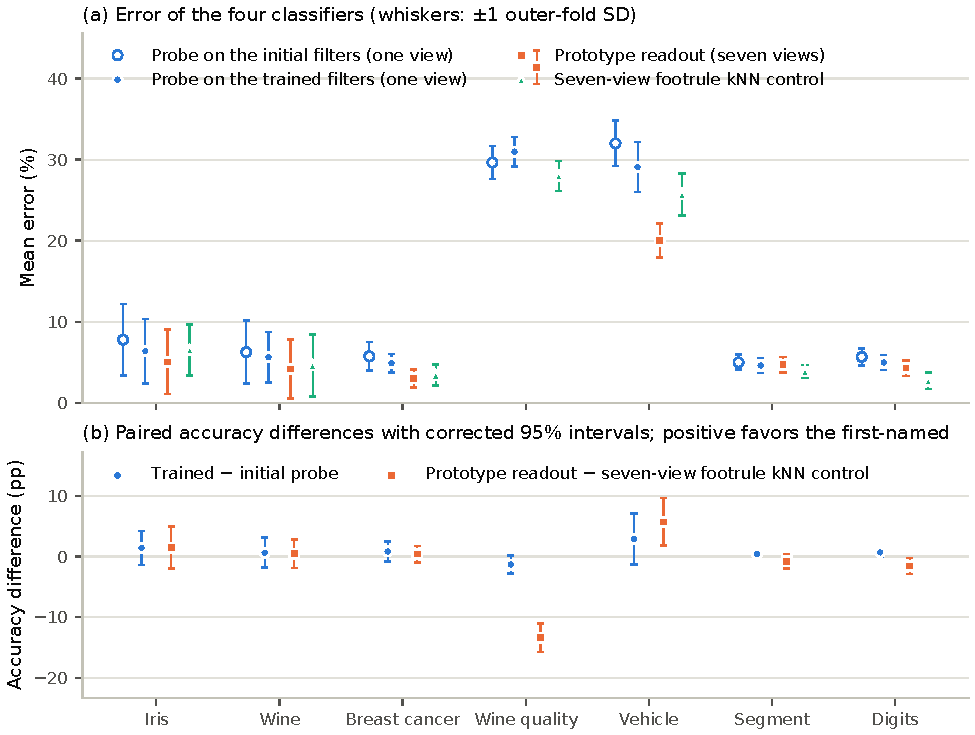
\includegraphics[width=\textwidth]{figures/data/fig7_learning_controls.pdf}
\caption{\textbf{Prototype-readout contrasts.} (a)~Mean outer-fold test error in percent on the seven benchmark datasets of four classifiers. A footrule kNN probe reads the hidden ranking of a single-view $[128]$ network before training (initial filters) and after training, with neighbor count and weighting chosen on inner folds (matched study). The others are the prototype readout with $K=7$ views and the seven-view footrule kNN control, footrule kNN on the same encoded views tuned on inner folds (component ablation). Whiskers are $\pm1$ outer-fold SD. (b)~The paired contrasts of Table~\ref{tab:contrasts}, trained minus initial probe and prototype readout minus kNN control, as accuracy differences in percentage points with 95\% corrected resampled-$t$ intervals (not simultaneous); positive favors the first-named. The prototype readout is at or above the kNN control on four datasets and below it on three. The trained probe is above the initial probe on six, and none of the seven probe intervals excludes zero. After Holm adjustment, one of the 14 contrasts remains significant (Wine quality prototype readout).}
\label{fig:learning-controls}
\end{figure}

% Rendered by render_tables.py from run files; do not edit by hand.
\begin{table}[!htbp]
\caption{\textbf{The 14 prototype-readout contrasts, fixed in the benchmark protocol before its outer folds were scored.} Paired accuracy differences in percentage points (first-named minus second-named; positive favors the first) on the seven benchmark datasets. Prototype readout $-$ seven-view footrule kNN control: the prototype readout with $K=7$ views against the seven-view footrule kNN control, footrule kNN on each of the same encoded views, tuned on inner folds and combined by majority vote (component ablation). Trained $-$ initial probe: a footrule kNN probe on the hidden ranking of the trained single-view $[128]$ network against the same probe on its initial filters (matched study). Each difference carries the 95\% corrected resampled-$t$ interval (test-to-training ratio 0.25, 14 degrees of freedom); intervals are not simultaneous, $p$ values are approximate, and the Holm column adjusts them over the family of 14. The prototype readout is at or above the kNN control on four datasets and the trained probe above the initial probe on six; three of the 14 intervals exclude zero, and one of the 14 contrasts remains significant after Holm adjustment.}
\label{tab:contrasts}
\centering
\footnotesize
\setlength{\tabcolsep}{3pt}
\begin{tabular}{lrrrr}
\toprule
Dataset & Difference (pp) & 95\% interval & $p$ & Holm $p$ \\
\midrule
\multicolumn{5}{l}{\emph{Prototype readout $-$ seven-view footrule kNN control}} \\
Iris & +1.5 & [$-$2.0, +4.9] & 0.374 & 1.000 \\
Wine & +0.4 & [$-$1.9, +2.8] & 0.693 & 1.000 \\
Breast cancer & +0.4 & [$-$1.0, +1.7] & 0.543 & 1.000 \\
Wine quality & $-$13.4 & [$-$15.7, $-$11.1] & $<$0.001 & $<$0.001 \\
Vehicle & +5.7 & [+1.8, +9.7] & 0.008 & 0.102 \\
Segment & $-$0.8 & [$-$2.0, +0.4] & 0.175 & 1.000 \\
Digits & $-$1.6 & [$-$2.9, $-$0.3] & 0.023 & 0.270 \\
\midrule
\multicolumn{5}{l}{\emph{Trained $-$ initial probe}} \\
Iris & +1.4 & [$-$1.4, +4.2] & 0.299 & 1.000 \\
Wine & +0.6 & [$-$1.9, +3.1] & 0.601 & 1.000 \\
Breast cancer & +0.8 & [$-$0.8, +2.5] & 0.292 & 1.000 \\
Wine quality & $-$1.3 & [$-$2.8, +0.2] & 0.081 & 0.810 \\
Vehicle & +2.9 & [$-$1.3, +7.1] & 0.160 & 1.000 \\
Segment & +0.4 & [$-$0.2, +1.0] & 0.168 & 1.000 \\
Digits & +0.7 & [$-$0.0, +1.4] & 0.059 & 0.654 \\
\bottomrule
\end{tabular}
\end{table}


The matched study looks at single-view networks in more detail. Table~\ref{tab:s-matched} reports the matched study on the seven benchmark datasets at every architecture. Table~\ref{tab:s-matched-controls} gives the reference classifiers on the same single encoded view. One of them, the hyperdimensional computing (HDC) control, is never trained. It works with bipolar vectors, whose entries are $+1$ and $-1$, in three steps. First, each item gets a fixed random bipolar key and each position a fixed bipolar code, nearby positions sharing most coordinates. Second, a ranking becomes the normalized sum over its positions of item key times position code. Third, each class vector is the normalized mean of its training vectors, and a query takes the class of highest cosine similarity. Cosine similarity is the cosine of the angle between two vectors. Nothing else is fitted.

Table~\ref{tab:s-contrasts} is the complete record of the 14 contrasts fixed in the prototype-readout protocol before its outer folds were scored. The matched protocol also declares its own family of 14 contrasts, two per dataset, with its own Holm adjustment. They set the trained probe against the initial one, and the prototype readout of the single-view network against fixed-configuration input footrule kNN. Table~\ref{tab:s-matched-family} reports this family for completeness, and no claim of this paper rests on it.

% Rendered by render_tables.py from run files; do not edit by hand.
\begin{table}[!htbp]
\caption{\textbf{Matched learning controls at every architecture (single view).} Mean outer-fold error in percent (outer-fold SD) on the seven benchmark datasets for the network's own prototype readout and for footrule kNN probes, tuned symmetrically on inner folds. The probes are applied to the hidden ranking of layer 1 and of the last hidden layer, of the trained network and of the same network before training (initial filters). One view per dataset, with learning rate 0.1, no augmentation and 200 iterations of batch size 32. Its encoder has degree $p=3$ with $e=16$ on Iris, $p=1$ with $e=64$ on Digits and $p=2$ with $e=32$ on the other five datasets. The validation fraction is 0.1 (the network trains on the remaining rows of each partition; probes and reference classifiers use every row). Protocol \texttt{arrowflow-v3-matched-1}.}
\label{tab:s-matched}
\centering
\scriptsize
\setlength{\tabcolsep}{3pt}
\resizebox{\ifdim\width>\linewidth\linewidth\else\width\fi}{!}{%
\begin{tabular}{llrrrrr}
\toprule
Dataset & Widths & Prototype readout & Probe, trained L1 & Probe, initial L1 & Probe, trained last & Probe, initial last \\
\midrule
Iris & $[128]$ & 11.2 (5.4) & 6.4 (4.0) & 7.8 (4.4) & (= layer 1) & (= layer 1) \\
 & $[64,128]$ & 10.7 (3.4) & 8.0 (4.3) & 7.9 (4.0) & 7.4 (4.1) & 8.1 (3.8) \\
 & $[64,32]$ & 9.3 (4.0) & 8.1 (4.5) & 8.3 (4.7) & 6.9 (3.4) & 9.3 (5.0) \\
\midrule
Wine & $[128]$ & 9.4 (4.1) & 5.6 (3.1) & 6.2 (3.9) & (= layer 1) & (= layer 1) \\
 & $[64,128]$ & 8.5 (5.6) & 7.2 (3.4) & 7.1 (3.2) & 6.1 (4.1) & 7.6 (3.9) \\
 & $[64,32]$ & 7.7 (3.3) & 6.7 (3.8) & 6.2 (3.7) & 6.2 (2.9) & 9.3 (3.3) \\
\midrule
Breast cancer & $[128]$ & 5.0 (1.5) & 4.9 (1.1) & 5.7 (1.8) & (= layer 1) & (= layer 1) \\
 & $[64,128]$ & 5.8 (1.5) & 5.7 (1.6) & 5.7 (1.6) & 5.1 (1.1) & 5.4 (1.2) \\
 & $[64,32]$ & 5.9 (1.6) & 5.4 (2.0) & 5.5 (1.9) & 5.3 (1.4) & 6.4 (2.0) \\
\midrule
Wine quality & $[128]$ & 48.8 (2.2) & 31.0 (1.8) & 29.6 (2.0) & (= layer 1) & (= layer 1) \\
 & $[64,128]$ & 49.7 (2.5) & 30.3 (2.1) & 29.7 (2.0) & 31.4 (1.7) & 29.9 (2.1) \\
 & $[64,32]$ & 49.8 (2.8) & 30.0 (2.2) & 29.9 (2.2) & 31.4 (1.9) & 30.4 (2.3) \\
\midrule
Vehicle & $[128]$ & 36.9 (2.4) & 29.1 (3.1) & 32.0 (2.8) & (= layer 1) & (= layer 1) \\
 & $[64,128]$ & 38.2 (3.0) & 32.6 (2.8) & 32.5 (2.7) & 32.9 (1.6) & 33.7 (3.5) \\
 & $[64,32]$ & 41.0 (2.7) & 32.7 (3.0) & 32.7 (3.1) & 34.0 (2.6) & 36.2 (3.2) \\
\midrule
Segment & $[128]$ & 12.1 (1.7) & 4.6 (0.9) & 5.0 (0.9) & (= layer 1) & (= layer 1) \\
 & $[64,128]$ & 12.7 (1.3) & 5.6 (1.1) & 5.3 (0.9) & 5.7 (1.0) & 5.6 (1.1) \\
 & $[64,32]$ & 14.5 (1.9) & 5.4 (1.0) & 5.3 (1.0) & 6.8 (1.1) & 7.0 (1.2) \\
\midrule
Digits & $[128]$ & 10.9 (1.5) & 5.0 (0.9) & 5.7 (1.1) & (= layer 1) & (= layer 1) \\
 & $[64,128]$ & 15.7 (0.9) & 7.1 (1.1) & 7.1 (1.0) & 8.2 (0.9) & 8.7 (1.4) \\
 & $[64,32]$ & 23.9 (2.4) & 7.1 (1.1) & 6.7 (1.2) & 13.8 (1.1) & 15.9 (1.1) \\
\bottomrule
\end{tabular}
}
\end{table}

% Rendered by render_tables.py from run files; do not edit by hand.
\begin{table}[!htbp]
\caption{\textbf{Reference classifiers on the same single encoded view.} Mean outer-fold error in percent (outer-fold SD) of the reference classifiers, each receiving the same encoded view as the networks of Table~\ref{tab:s-matched}. The first is fixed-configuration input footrule kNN: footrule kNN on the input rankings of this encoded view, with neighbors and weights tuned on inner folds. The others are the mean-position prototype classifier (one Borda prototype per class, nearest by footrule) and an ordered-position hyperdimensional computing (HDC) control. The HDC control has dimension 1,024 or 10,000, chosen on inner folds. Footrule kNN has the lowest error of the three on every dataset.}
\label{tab:s-matched-controls}
\centering
\footnotesize
\setlength{\tabcolsep}{3pt}
\begin{tabular}{lrrr}
\toprule
Dataset & Fixed-configuration input footrule kNN & Borda prototype & HDC \\
\midrule
Iris & 7.6 (5.3) & 16.4 (6.6) & 12.4 (6.7) \\
Wine & 6.6 (4.0) & 9.9 (5.3) & 7.2 (4.5) \\
Breast cancer & 5.6 (2.6) & 9.0 (2.4) & 9.0 (2.1) \\
Wine quality & 29.0 (2.4) & 49.1 (3.1) & 46.8 (2.7) \\
Vehicle & 31.3 (3.0) & 51.5 (3.4) & 50.9 (3.5) \\
Segment & 4.8 (0.8) & 21.5 (2.7) & 18.2 (2.1) \\
Digits & 4.3 (1.2) & 16.3 (2.0) & 13.8 (2.1) \\
\bottomrule
\end{tabular}
\end{table}


In Tables~\ref{tab:s-matched} and~\ref{tab:s-matched-controls}, at the primary architecture $[128]$ the network's prototype readout has lower error than footrule kNN on the input rankings only on Breast cancer ($5.0$ against $5.6\%$). On the other six datasets its error is higher, by $2.8$ (Wine) to $19.7$ points (Wine quality). On Wine quality, Segment and Digits, the prototype readout has $48.8$, $12.1$ and $10.9\%$ error. The trained probe on its hidden ranking has $31.0$, $4.6$ and $5.0\%$, and footrule kNN on the input rankings has $29.0$, $4.8$ and $4.3\%$. There the probe's error is within $2.0$ points of that of footrule kNN on the input rankings, a descriptive difference. The prototype readout has higher error than both. In Table~\ref{tab:s-matched}, the lowest prototype-readout error comes from $[128]$ on five datasets and from $[64,32]$ on Iris and Wine.

For the two-layer networks, we can also probe each hidden layer. The probe on the trained last hidden layer has error at most equal to that of the probe on the initial one in 11 of 14 pairs of dataset and architecture. The exceptions are Wine quality (both architectures) and Segment ($[64,128]$). The probe on the trained last hidden layer has higher error than the probe on the trained first layer on Wine quality, Vehicle, Segment and Digits at both two-layer architectures, and lower error on Iris, Wine and Breast cancer.

% Rendered by render_tables.py from run files; do not edit by hand.
\begin{table}[!htbp]
\caption{\textbf{Complete record of the 14 contrasts fixed in the benchmark protocol before its outer folds were scored.} Family index, dataset, contrast, source family, mean paired accuracy difference in percentage points, its standard error (SE) in points, the 95\% corrected resampled-$t$ interval (test-to-training ratio 0.25, 14 degrees of freedom), the approximate $p$ value and the Holm-adjusted $p$ value over the family of 14. Every member is computed, and one Holm adjustment covers the family.}
\label{tab:s-contrasts}
\centering
\scriptsize
\setlength{\tabcolsep}{3pt}
\resizebox{\ifdim\width>\linewidth\linewidth\else\width\fi}{!}{%
\begin{tabular}{rlllrrrrr}
\toprule
\# & Dataset & Contrast & Source & Diff. (pp) & SE & 95\% interval & $p$ & Holm $p$ \\
\midrule
1 & Iris & Prototype readout $-$ seven-view footrule kNN control & component ablation & +1.5 & 1.6 & [$-$2.0, +4.9] & 0.374 & 1.000 \\
2 & Wine & Prototype readout $-$ seven-view footrule kNN control & component ablation & +0.4 & 1.1 & [$-$1.9, +2.8] & 0.693 & 1.000 \\
3 & Breast cancer & Prototype readout $-$ seven-view footrule kNN control & component ablation & +0.4 & 0.6 & [$-$1.0, +1.7] & 0.543 & 1.000 \\
4 & Wine quality & Prototype readout $-$ seven-view footrule kNN control & component ablation & $-$13.4 & 1.1 & [$-$15.7, $-$11.1] & $<$0.001 & $<$0.001 \\
5 & Vehicle & Prototype readout $-$ seven-view footrule kNN control & component ablation & +5.7 & 1.8 & [+1.8, +9.7] & 0.008 & 0.102 \\
6 & Segment & Prototype readout $-$ seven-view footrule kNN control & component ablation & $-$0.8 & 0.6 & [$-$2.0, +0.4] & 0.175 & 1.000 \\
7 & Digits & Prototype readout $-$ seven-view footrule kNN control & component ablation & $-$1.6 & 0.6 & [$-$2.9, $-$0.3] & 0.023 & 0.270 \\
\midrule
8 & Iris & Trained $-$ initial probe & matched study & +1.4 & 1.3 & [$-$1.4, +4.2] & 0.299 & 1.000 \\
9 & Wine & Trained $-$ initial probe & matched study & +0.6 & 1.2 & [$-$1.9, +3.1] & 0.601 & 1.000 \\
10 & Breast cancer & Trained $-$ initial probe & matched study & +0.8 & 0.8 & [$-$0.8, +2.5] & 0.292 & 1.000 \\
11 & Wine quality & Trained $-$ initial probe & matched study & $-$1.3 & 0.7 & [$-$2.8, +0.2] & 0.081 & 0.810 \\
12 & Vehicle & Trained $-$ initial probe & matched study & +2.9 & 2.0 & [$-$1.3, +7.1] & 0.160 & 1.000 \\
13 & Segment & Trained $-$ initial probe & matched study & +0.4 & 0.3 & [$-$0.2, +1.0] & 0.168 & 1.000 \\
14 & Digits & Trained $-$ initial probe & matched study & +0.7 & 0.3 & [$-$0.0, +1.4] & 0.059 & 0.654 \\
\bottomrule
\end{tabular}
}
\end{table}

% Rendered by render_tables.py from run files; do not edit by hand.
\begin{table}[!htbp]
\caption{\textbf{Contrast family of the matched protocol.} The matched protocol declared these fourteen contrasts, two per dataset, with one Holm adjustment over them. The first is the footrule kNN probe on the trained hidden ranking of the single-view $[128]$ network minus the same probe on its initial filters; the second is that network's prototype readout minus fixed-configuration input footrule kNN. Differences are in percentage points with the 95\% corrected resampled-$t$ interval (test-to-training ratio 0.25, 14 degrees of freedom); $p$ values are approximate. The probe contrasts equal those of Table~\ref{tab:s-contrasts}, whose family adjusts them together with the seven-view control instead. This family is reported for completeness, and no claim of this paper rests on it. Four of the fourteen contrasts remain significant after Holm adjustment, each a prototype readout below fixed-configuration input footrule kNN.}
\label{tab:s-matched-family}
\centering
\scriptsize
\setlength{\tabcolsep}{3pt}
\resizebox{\ifdim\width>\linewidth\linewidth\else\width\fi}{!}{%
\begin{tabular}{llrrrr}
\toprule
Dataset & Contrast & Difference (pp) & 95\% interval & $p$ & Holm $p$ \\
\midrule
Iris & Trained $-$ initial probe & +1.4 & [$-$1.4, +4.2] & 0.299 & 1.000 \\
 & Prototype readout $-$ fixed-configuration input footrule kNN & $-$3.6 & [$-$11.5, +4.2] & 0.338 & 1.000 \\
\midrule
Wine & Trained $-$ initial probe & +0.6 & [$-$1.9, +3.1] & 0.601 & 1.000 \\
 & Prototype readout $-$ fixed-configuration input footrule kNN & $-$2.8 & [$-$8.0, +2.4] & 0.265 & 1.000 \\
\midrule
Breast cancer & Trained $-$ initial probe & +0.8 & [$-$0.8, +2.5] & 0.292 & 1.000 \\
 & Prototype readout $-$ fixed-configuration input footrule kNN & +0.6 & [$-$1.9, +3.1] & 0.613 & 1.000 \\
\midrule
Wine quality & Trained $-$ initial probe & $-$1.3 & [$-$2.8, +0.2] & 0.081 & 0.729 \\
 & Prototype readout $-$ fixed-configuration input footrule kNN & $-$19.7 & [$-$22.9, $-$16.6] & $<$0.001 & $<$0.001 \\
\midrule
Vehicle & Trained $-$ initial probe & +2.9 & [$-$1.3, +7.1] & 0.160 & 1.000 \\
 & Prototype readout $-$ fixed-configuration input footrule kNN & $-$5.6 & [$-$8.3, $-$2.9] & $<$0.001 & 0.007 \\
\midrule
Segment & Trained $-$ initial probe & +0.4 & [$-$0.2, +1.0] & 0.168 & 1.000 \\
 & Prototype readout $-$ fixed-configuration input footrule kNN & $-$7.3 & [$-$9.3, $-$5.3] & $<$0.001 & $<$0.001 \\
\midrule
Digits & Trained $-$ initial probe & +0.7 & [$-$0.0, +1.4] & 0.059 & 0.594 \\
 & Prototype readout $-$ fixed-configuration input footrule kNN & $-$6.6 & [$-$8.7, $-$4.5] & $<$0.001 & $<$0.001 \\
\bottomrule
\end{tabular}
}
\end{table}


\clearpage
\subsection{Details for Section~\ref*{sec:motion-controls}: Matched Motion-Signal Controls}\label{supp:motion}

This subsection and the next hold the complete numerical record of the eight controlled experiments summarized in Sections~\ref{sec:motion-controls} and~\ref{sec:controlled}. Every one of them reuses the split seed, the fitting seeds and the outer and inner folds of the registered runs. So each contrast is paired fold by fold with the run it is compared against. None of them changes the seventeen-dataset results of Sections~\ref{supp:benchmark} and~\ref{supp:training}, which stand as registered.

Each family carries its own Holm adjustment over its own contrasts. Every rate pooled over folds, repeats and fitting seeds is descriptive. Pooled rates count the same test rows more than once, so none of them receives an interval or a test. Section~\ref{supp:reproducibility} gives the protocol file, the code revision and the commands of each family.

\paragraph{Design.} These arms, the controls of Section~\ref{sec:motion-controls}, ask whether the particular signal the output layer returns carries information, or whether movement of the same size would serve as well. On most datasets, a scrambled signal leaves the network less accurate than frozen filters, so the signal does carry information. The arms change only what reaches the hidden filters. They hold everything else fixed: the encoder family and its selection, the nearest-neighbor readout, the seven views, the folds and the fitting seeds. The iteration count stays fixed too, and so does the eligibility gate that decides which training rows are accepted. Each arm applies the gate's rule to its own prototype readout, so its gate decisions are recomputed, not replayed.

An unmodified arm is fitted through the same instrumentation wrapper with an identity transform, one that leaves every motion as it is. It has to reproduce the reference run's outer predictions on every fold and seed. This check shows that the wrapper itself has no effect on the fit.

The frozen arm never applies the accumulated motion to its hidden filters. It asks whether the hidden filters need to move at all, and it cannot say whether their particular movement makes a difference. The frozen arm is not the untrained ArrowFlow of Section~\ref{supp:training}. That control never trains any layer, so its training settings have no effect. It also selects its own configuration. The readout reads only the hidden layers, so the frozen arm predicts exactly as the untrained networks of the component ablation (Section~\ref{supp:ablation-arrowflow}). Its column of Table~\ref{tab:s-motion-family} therefore equals that variant's column of Table~\ref{tab:s-components-changes}. Those results existed before this protocol was frozen, so only the two scrambling arms were scored blind.

The permuted-alignment arm keeps every motion record with its magnitude and sign. But it reassigns each record by a random permutation of the layer's filter identities. So it changes only which filter receives each motion. The permutation is drawn anew for every layer and batch. A fixed permutation, the permutation analog of feedback alignment \citep{lillicrap2016random}, was not tested. Feedback alignment trains a neural network by sending its errors back through fixed random weights, where backpropagation would reuse the forward weights.

The random-direction arm changes the directions instead. An attracting vote pulls a filter toward the batch input, and a repelling vote pushes it away. The arm shuffles the signs of the nonzero votes among their slots, within each record, layer and batch. A slot is one filter that one example selects in one batch. The shuffle keeps exactly the slots, the vote mass (the total vote weight) per batch and layer, the vote magnitudes with their repeats and the counts of attraction and repulsion. Only the pairing of each filter with its direction is broken. The arm leaves the mix of attraction and repulsion alone on purpose, because a changed mix would confound the comparison.

The two scrambles differ in strength. About half of the nonzero votes attract, so the random-direction arm reverses the direction of about half of them. Permuted alignment instead moves almost every selected slot, zero votes included, to another filter. Table~\ref{tab:s-motion-statistics} records both rates per dataset and layer. It also gives the share of each run's slots that carry a vote and the share of ArrowFlow's votes that repel, which is about half on every dataset and layer.

Every arm keeps the class-filter target and the error gate. The controls therefore show that it makes a difference which filter each motion reaches and in which direction. But they do not tell apart information from the labels and structure that any consistent target would impose. A full permutation of the class labels is a different experiment and is not claimed here.

Table~\ref{tab:s-motion-family} holds the primary family, the three arms on all seventeen datasets. Its contrasts are Holm-adjusted across the datasets within each arm, and the arms are adjusted separately. The protocol declared this before its own outer folds were scored. As noted above, the frozen arm's results existed earlier. Table~\ref{tab:s-motion-scramble} compares each scramble with the frozen arm directly, a comparison the protocol did not declare. Post hoc, an exact one-sided signed-rank test \citep{demsar2006statistical} across the seventeen datasets supports both scrambles being less accurate than frozen filters ($p<0.001$ for each). Table~\ref{tab:s-motion-purity} gives the same-class purity of the last hidden ranking for the test and the training rows of every arm. Purity is the share of a row's nearest stored training rankings that carry its class, so it measures the neighborhoods that the readout reads. The purity table is descriptive and carries no test.

Table~\ref{tab:s-motion-single-layer} holds two further arms that train only the first, or only the last, hidden layer. When a fold selected one hidden layer, both arms equal the unmodified run by construction. So each row uses only the outer folds whose selection has two hidden layers. No dataset selected two hidden layers on every outer fold, and several selected them on none. These arms therefore sit outside the primary family and are not Holm-adjusted. Every row prints its fold count.

\paragraph{Results.} On most datasets, training makes the neighborhoods purer, and either scramble makes them less pure than frozen filters. ArrowFlow's neighborhoods are purer than those of the frozen arm on 13 of the 17 datasets, and the permuted-alignment and random-direction arms leave them less pure than the frozen arm on 15 and 14 of the 17. No arm differs detectably on HCV, where no model beats the majority class, and its purities are essentially unchanged. The two scrambling arms change the votes in different ways and by different amounts (Table~\ref{tab:s-motion-statistics}). So each is read against the frozen arm, and the two are not compared with each other.

\clearpage
% Rendered by render_tables.py from run files; do not edit by hand.
\begin{table}[!htbp]
\caption{\textbf{Matched motion-signal controls: the primary family.} ArrowFlow minus the control arm, accuracy, in percentage points, on the seventeen datasets. Fitting seeds are averaged within each outer fold; intervals are 95\% corrected resampled-$t$ interval (test-to-training ratio 0.25, 14 degrees of freedom). Positive favors ArrowFlow. Holm adjusts across the seventeen datasets within each arm, the three arms separately, as the run protocol declared before its own outer folds were scored. The frozen arm predicts exactly as the untrained networks of the component ablation (Table~\ref{tab:s-components-changes}), whose results existed before this protocol was frozen, so only the two scrambling arms were scored blind. The permuted-alignment arm is less accurate than the frozen arm on 16 of the 17 datasets and the random-direction arm on 14 of the 17. Holm adjustment leaves 3 datasets significant in the frozen filters arm, 5 in the permuted alignment arm and 3 in the random directions arm. kNN: nearest-neighbor classifier; HCV: hepatitis C virus.}
\label{tab:s-motion-family}
\centering
\scriptsize
\setlength{\tabcolsep}{3pt}
\resizebox{\ifdim\width>\linewidth\linewidth\else\width\fi}{!}{%
\begin{tabular}{lrrrrrr}
\toprule
Dataset & \begin{tabular}[b]{@{}r@{}}Frozen\\Diff. (pp)\end{tabular} & \begin{tabular}[b]{@{}r@{}}Frozen\\95\% interval\end{tabular} & \begin{tabular}[b]{@{}r@{}}Frozen\\Holm $p$\end{tabular} & \begin{tabular}[b]{@{}r@{}}Permuted\\Diff. (pp)\end{tabular} & \begin{tabular}[b]{@{}r@{}}Permuted\\95\% interval\end{tabular} & \begin{tabular}[b]{@{}r@{}}Permuted\\Holm $p$\end{tabular} \\
\midrule
Iris & +0.52 & [$-$1.68, +2.72] & 1.000 & +0.96 & [$-$1.06, +2.98] & 1.000 \\
Wine & +0.68 & [$-$2.06, +3.41] & 1.000 & +0.87 & [$-$1.36, +3.10] & 1.000 \\
Breast cancer & +0.84 & [$-$0.45, +2.13] & 1.000 & +0.78 & [$-$0.49, +2.05] & 1.000 \\
Wine quality & +0.02 & [$-$1.03, +1.08] & 1.000 & +0.51 & [$-$0.82, +1.83] & 1.000 \\
Vehicle & +3.61 & [+1.18, +6.05] & 0.093 & +6.69 & [+3.15, +10.23] & 0.018 \\
Segment & +1.20 & [+0.54, +1.86] & 0.023 & +1.40 & [+0.65, +2.16] & 0.020 \\
Digits & +0.15 & [$-$0.89, +1.19] & 1.000 & +1.17 & [+0.29, +2.06] & 0.156 \\
balance-scale & +5.35 & [+3.39, +7.31] & $<$0.001 & +6.97 & [+4.38, +9.55] & $<$0.001 \\
mfeat-zernike & +2.47 & [+1.45, +3.49] & 0.002 & +7.06 & [+5.75, +8.37] & $<$0.001 \\
ionosphere & +0.19 & [$-$2.99, +3.37] & 1.000 & +1.90 & [$-$0.93, +4.73] & 1.000 \\
vertebra-column & +0.65 & [$-$2.74, +4.03] & 1.000 & +1.18 & [$-$1.63, +3.99] & 1.000 \\
diabetes & $-$0.15 & [$-$1.71, +1.42] & 1.000 & +0.92 & [$-$0.38, +2.22] & 1.000 \\
banknote-authentication & $-$0.02 & [$-$0.25, +0.22] & 1.000 & +0.03 & [$-$0.05, +0.12] & 1.000 \\
qsar-biodeg & +1.26 & [+0.32, +2.21] & 0.159 & +2.12 & [+0.86, +3.37] & 0.037 \\
steel-plates-fault & +0.96 & [$-$1.04, +2.96] & 1.000 & +2.16 & [$-$0.38, +4.71] & 0.981 \\
climate-model-simulation-crashes & +0.06 & [$-$0.32, +0.44] & 1.000 & +0.16 & [$-$0.28, +0.61] & 1.000 \\
HCV & $-$0.02 & [$-$1.79, +1.76] & 1.000 & +0.17 & [$-$1.95, +2.29] & 1.000 \\
\bottomrule
\end{tabular}
}
\par\medskip
\resizebox{\ifdim\width>\linewidth\linewidth\else\width\fi}{!}{%
\begin{tabular}{lrrr}
\toprule
Dataset & \begin{tabular}[b]{@{}r@{}}Random\\Diff. (pp)\end{tabular} & \begin{tabular}[b]{@{}r@{}}Random\\95\% interval\end{tabular} & \begin{tabular}[b]{@{}r@{}}Random\\Holm $p$\end{tabular} \\
\midrule
Iris & +0.81 & [$-$1.36, +2.99] & 1.000 \\
Wine & +1.24 & [$-$0.44, +2.92] & 1.000 \\
Breast cancer & +0.74 & [$-$0.56, +2.04] & 1.000 \\
Wine quality & +0.33 & [$-$0.76, +1.41] & 1.000 \\
Vehicle & +6.49 & [+2.91, +10.07] & 0.024 \\
Segment & +1.42 & [+0.48, +2.36] & 0.079 \\
Digits & +0.34 & [$-$0.63, +1.31] & 1.000 \\
balance-scale & +6.35 & [+4.03, +8.67] & $<$0.001 \\
mfeat-zernike & +4.56 & [+3.27, +5.84] & $<$0.001 \\
ionosphere & +1.64 & [$-$0.92, +4.21] & 1.000 \\
vertebra-column & +0.57 & [$-$2.22, +3.36] & 1.000 \\
diabetes & +0.14 & [$-$1.59, +1.88] & 1.000 \\
banknote-authentication & +0.00 & [$-$0.23, +0.23] & 1.000 \\
qsar-biodeg & +1.86 & [+0.68, +3.04] & 0.062 \\
steel-plates-fault & +1.66 & [$-$0.63, +3.95] & 1.000 \\
climate-model-simulation-crashes & +0.16 & [$-$0.25, +0.58] & 1.000 \\
HCV & $-$0.14 & [$-$2.21, +1.92] & 1.000 \\
\bottomrule
\end{tabular}
}
\end{table}

% Rendered by render_tables.py from run files; do not edit by hand.
\begin{table}[!htbp]
\caption{\textbf{Matched motion-signal controls: each scramble against frozen filters (post hoc).} The mean accuracy of each scrambling arm minus that of the frozen arm, in percentage points, per dataset; negative means that the scrambled signal left the network less accurate than frozen filters. The values are differences of the arm accuracies of Table~\ref{tab:s-motion-family}, so they carry no interval. The protocol declared ArrowFlow minus each arm, not this comparison. The test ranks the seventeen absolute differences, and its $p$ value is the share of the $2^{17}$ sign assignments whose sum of positive ranks is at most the observed one. Post hoc, an exact one-sided Wilcoxon signed-rank test across the seventeen datasets gives $p=2.3\times10^{-5}$ for permuted alignment, below the frozen arm on 16 of the 17 datasets, and $p=3.3\times10^{-4}$ for random directions, below it on 14 of the 17. HCV: hepatitis C virus.}
\label{tab:s-motion-scramble}
\centering
\scriptsize
\setlength{\tabcolsep}{3pt}
\begin{tabular}{lrr}
\toprule
Dataset & \begin{tabular}[b]{@{}r@{}}Permuted\\$-$ frozen (pp)\end{tabular} & \begin{tabular}[b]{@{}r@{}}Random\\$-$ frozen (pp)\end{tabular} \\
\midrule
Iris & $-$0.44 & $-$0.30 \\
Wine & $-$0.19 & $-$0.56 \\
Breast cancer & +0.06 & +0.10 \\
Wine quality & $-$0.49 & $-$0.31 \\
Vehicle & $-$3.07 & $-$2.88 \\
Segment & $-$0.20 & $-$0.22 \\
Digits & $-$1.03 & $-$0.19 \\
balance-scale & $-$1.62 & $-$1.00 \\
mfeat-zernike & $-$4.59 & $-$2.09 \\
ionosphere & $-$1.70 & $-$1.45 \\
vertebra-column & $-$0.54 & +0.07 \\
diabetes & $-$1.07 & $-$0.29 \\
banknote-authentication & $-$0.05 & $-$0.02 \\
qsar-biodeg & $-$0.85 & $-$0.60 \\
steel-plates-fault & $-$1.20 & $-$0.70 \\
climate-model-simulation-crashes & $-$0.10 & $-$0.10 \\
HCV & $-$0.18 & +0.13 \\
\bottomrule
\end{tabular}
\end{table}

% Rendered by render_tables.py from run files; do not edit by hand.
\begin{table}[!htbp]
\caption{\textbf{Matched motion-signal controls: neighborhood purity.} Same-class purity of the last hidden ranking, in percent. For each row it is the share of its nearest stored training rankings that carry its class, at the neighbor count the view selected. Rows are averaged first, then the seven views, then the outer folds. Training rows drop their own stored ranking and are subsampled above 512 rows. Descriptive: no test and no interval. On balance-scale the purity of the outer test rows is 89.72 percent for ArrowFlow, 77.61 for the frozen filters, 73.85 for the permuted alignment and 75.17 for the random directions. HCV: hepatitis C virus.}
\label{tab:s-motion-purity}
\centering
\scriptsize
\setlength{\tabcolsep}{3pt}
\resizebox{\ifdim\width>\linewidth\linewidth\else\width\fi}{!}{%
\begin{tabular}{lrrrrrrrr}
\toprule
Dataset & \begin{tabular}[b]{@{}r@{}}ArrowFlow\\Test\end{tabular} & \begin{tabular}[b]{@{}r@{}}ArrowFlow\\Training\end{tabular} & \begin{tabular}[b]{@{}r@{}}Frozen\\Test\end{tabular} & \begin{tabular}[b]{@{}r@{}}Frozen\\Training\end{tabular} & \begin{tabular}[b]{@{}r@{}}Permuted\\Test\end{tabular} & \begin{tabular}[b]{@{}r@{}}Permuted\\Training\end{tabular} & \begin{tabular}[b]{@{}r@{}}Random\\Test\end{tabular} & \begin{tabular}[b]{@{}r@{}}Random\\Training\end{tabular} \\
\midrule
Iris & 92.10 & 92.69 & 91.59 & 91.91 & 90.44 & 90.67 & 90.99 & 91.36 \\
Wine & 94.15 & 95.58 & 90.68 & 91.13 & 92.64 & 93.31 & 91.90 & 92.32 \\
Breast cancer & 95.47 & 96.44 & 93.83 & 94.14 & 94.15 & 94.52 & 93.98 & 94.31 \\
Wine quality & 52.09 & 52.54 & 52.31 & 52.49 & 51.67 & 51.79 & 51.96 & 52.11 \\
Vehicle & 71.41 & 74.24 & 68.37 & 69.74 & 64.03 & 65.63 & 65.28 & 66.62 \\
Segment & 96.60 & 96.75 & 95.71 & 95.86 & 94.88 & 95.07 & 95.14 & 95.29 \\
Digits & 94.74 & 96.23 & 94.23 & 94.25 & 92.63 & 92.69 & 94.03 & 94.15 \\
balance-scale & 89.72 & 90.37 & 77.61 & 77.68 & 73.85 & 73.90 & 75.17 & 75.15 \\
mfeat-zernike & 78.13 & 79.25 & 75.22 & 74.90 & 69.18 & 68.99 & 72.28 & 72.04 \\
ionosphere & 86.05 & 88.18 & 85.66 & 86.51 & 83.54 & 84.89 & 83.97 & 84.89 \\
vertebra-column & 76.57 & 77.80 & 74.99 & 75.23 & 74.64 & 75.19 & 74.95 & 75.22 \\
diabetes & 67.29 & 67.83 & 67.21 & 67.47 & 66.73 & 67.12 & 66.89 & 67.19 \\
banknote-authentication & 99.54 & 99.62 & 99.46 & 99.53 & 99.43 & 99.49 & 99.48 & 99.55 \\
qsar-biodeg & 79.83 & 79.88 & 79.30 & 79.04 & 78.89 & 78.75 & 79.22 & 79.04 \\
steel-plates-fault & 66.39 & 67.79 & 66.93 & 67.46 & 64.29 & 64.65 & 65.86 & 66.24 \\
climate-model-simulation-crashes & 85.43 & 86.58 & 87.13 & 87.29 & 86.63 & 86.73 & 86.80 & 86.94 \\
HCV & 24.92 & 28.05 & 24.95 & 26.36 & 24.94 & 25.73 & 24.92 & 25.84 \\
\bottomrule
\end{tabular}
}
\end{table}

% Rendered by render_tables.py from run files; do not edit by hand.
\begin{table}[!htbp]
\caption{\textbf{Matched motion-signal controls: what each arm changed.} Counts over every fold, seed and view, per dataset and hidden layer; layer 1 is the first hidden layer. A slot is one filter that one example selects in one batch: every example of every batch selects $\lceil\rho N_\ell\rceil$ filters of each hidden layer, and an example that the gate rejects gives its slots zero votes. Selected slots: their number in millions, the same in every arm. Nonzero: the share of the selected slots that carry a nonzero vote, in the arm's own run. Repulsions: the share of ArrowFlow's nonzero votes that push a filter away from the batch input rather than pull it toward it. Moved: the share of all selected slots, zero votes included, that permuted alignment delivers to another filter. Reversed: the share of the random-direction arm's nonzero votes whose direction it reverses; permuting the signs of votes of which a share $q$ attract reverses a share $2q(1-q)$ on average. Both arms preserve the slots, the vote magnitudes and the vote mass of every batch exactly. Among ArrowFlow's nonzero votes, repulsions make up about half, 49.87 to 50.12 percent, on every dataset and layer, and the random-direction arm reverses 49.74 to 49.90 percent of its nonzero votes. On balance-scale permuted alignment moves 99.23 percent of the selected slots to another filter, and random directions reverses 49.87 percent of its nonzero votes, which are 17.67 percent of the selected slots, so the two arms are not equally strong.}
\label{tab:s-motion-statistics}
\centering
\scriptsize
\setlength{\tabcolsep}{3pt}
\begin{tabular}{llrrrrrr}
\toprule
Dataset & Layer & \begin{tabular}[b]{@{}r@{}}Selected\\slots (M)\end{tabular} & \begin{tabular}[b]{@{}r@{}}ArrowFlow:\\nonzero (\%)\end{tabular} & \begin{tabular}[b]{@{}r@{}}ArrowFlow:\\repulsions (\%)\end{tabular} & \begin{tabular}[b]{@{}r@{}}Permuted:\\moved (\%)\end{tabular} & \begin{tabular}[b]{@{}r@{}}Random:\\nonzero (\%)\end{tabular} & \begin{tabular}[b]{@{}r@{}}Random:\\reversed (\%)\end{tabular} \\
\midrule
Iris & 1 & 98.9 & 4.00 & 49.98 & 98.99 & 6.84 & 49.81 \\
Iris & 2 & 60.2 & 4.27 & 50.08 & 99.22 & 7.34 & 49.80 \\
\midrule
Wine & 1 & 81.7 & 1.94 & 50.01 & 98.76 & 4.24 & 49.77 \\
Wine & 2 & 94.6 & 2.11 & 50.01 & 99.22 & 4.54 & 49.85 \\
\midrule
Breast cancer & 1 & 111.8 & 3.63 & 49.98 & 99.10 & 4.51 & 49.83 \\
Breast cancer & 2 & 34.4 & 4.12 & 50.06 & 99.22 & 5.07 & 49.89 \\
\midrule
Wine quality & 1 & 129.0 & 54.30 & 49.87 & 99.21 & 47.98 & 49.86 \\
\midrule
Vehicle & 1 & 116.1 & 36.81 & 49.99 & 99.13 & 41.55 & 49.86 \\
Vehicle & 2 & 25.8 & 30.70 & 50.12 & 99.21 & 40.36 & 49.88 \\
\midrule
Segment & 1 & 129.0 & 15.40 & 50.05 & 99.22 & 27.28 & 49.85 \\
\midrule
Digits & 1 & 129.0 & 10.02 & 50.07 & 99.22 & 38.78 & 49.86 \\
\midrule
balance-scale & 1 & 129.0 & 10.47 & 50.08 & 99.23 & 17.67 & 49.87 \\
\midrule
mfeat-zernike & 1 & 129.0 & 26.65 & 50.06 & 99.22 & 54.70 & 49.87 \\
\midrule
ionosphere & 1 & 111.8 & 15.50 & 50.00 & 99.10 & 19.11 & 49.85 \\
ionosphere & 2 & 34.4 & 31.73 & 50.07 & 99.22 & 24.04 & 49.90 \\
\midrule
vertebra-column & 1 & 81.7 & 21.97 & 50.01 & 98.77 & 21.58 & 49.74 \\
vertebra-column & 2 & 94.6 & 21.70 & 50.05 & 99.23 & 21.66 & 49.77 \\
\midrule
diabetes & 1 & 107.5 & 41.45 & 49.94 & 99.06 & 33.70 & 49.86 \\
diabetes & 2 & 43.0 & 47.65 & 50.02 & 99.23 & 34.50 & 49.88 \\
\midrule
banknote-authentication & 1 & 90.3 & 4.49 & 50.01 & 98.88 & 6.27 & 49.76 \\
banknote-authentication & 2 & 77.4 & 5.31 & 50.02 & 99.23 & 7.11 & 49.82 \\
\midrule
qsar-biodeg & 1 & 129.0 & 33.91 & 49.94 & 99.22 & 28.75 & 49.85 \\
\midrule
steel-plates-fault & 1 & 129.0 & 40.09 & 50.03 & 99.22 & 53.77 & 49.87 \\
\midrule
climate-model-simulation-crashes & 1 & 107.5 & 35.41 & 50.01 & 99.06 & 34.89 & 49.85 \\
climate-model-simulation-crashes & 2 & 43.0 & 31.02 & 50.05 & 99.22 & 33.66 & 49.87 \\
\midrule
HCV & 1 & 81.7 & 66.92 & 49.93 & 98.76 & 70.69 & 49.77 \\
HCV & 2 & 94.6 & 67.66 & 50.08 & 99.22 & 70.96 & 49.88 \\
\bottomrule
\end{tabular}
\end{table}

% Rendered by render_tables.py from run files; do not edit by hand.
\begin{table}[!htbp]
\caption{\textbf{Matched motion-signal controls: one hidden layer trained.} ArrowFlow minus an arm in which only the first, or only the last, hidden layer applies its accumulated motion, accuracy, in percentage points. At a one-hidden-layer selection the arm is ArrowFlow by construction, so each row uses only the outer folds whose selection has two hidden layers; the second column gives their number $n$. Intervals are 95\% corrected resampled-$t$ intervals over the $n$ folds of a row, with the variance of the fold differences multiplied by $1/n+0.25$ and $n-1$ degrees of freedom; the $p$ values use the same $t$ distribution. Every fold difference is zero in the last-only row of climate-model-simulation-crashes, which therefore has no interval and no test. Descriptive: not part of the primary family and not Holm-adjusted. Seven of the seventeen datasets selected two hidden layers on no outer fold, so their rows are empty.}
\label{tab:s-motion-single-layer}
\centering
\scriptsize
\setlength{\tabcolsep}{3pt}
\resizebox{\ifdim\width>\linewidth\linewidth\else\width\fi}{!}{%
\begin{tabular}{llrrrrrr}
\toprule
Dataset & \begin{tabular}[b]{@{}r@{}}Two-layer\\folds\end{tabular} & \begin{tabular}[b]{@{}r@{}}First only\\Diff. (pp)\end{tabular} & \begin{tabular}[b]{@{}r@{}}First only\\95\% interval\end{tabular} & \begin{tabular}[b]{@{}r@{}}First only\\$p$\end{tabular} & \begin{tabular}[b]{@{}r@{}}Last only\\Diff. (pp)\end{tabular} & \begin{tabular}[b]{@{}r@{}}Last only\\95\% interval\end{tabular} & \begin{tabular}[b]{@{}r@{}}Last only\\$p$\end{tabular} \\
\midrule
Iris & 7 of 15 & +0.32 & [$-$1.30, +1.94] & 0.649 & $-$0.32 & [$-$1.61, +0.97] & 0.569 \\
Wine & 11 of 15 & +1.61 & [$-$1.26, +4.48] & 0.240 & +0.00 & [$-$1.33, +1.33] & 0.997 \\
Breast cancer & 4 of 15 & +0.36 & [$-$2.29, +3.02] & 0.691 & $-$0.22 & [$-$2.12, +1.68] & 0.735 \\
Wine quality & 0 of 15 & -- & -- & -- & -- & -- & -- \\
Vehicle & 3 of 15 & +1.37 & [$-$6.68, +9.42] & 0.540 & $-$2.23 & [$-$4.52, +0.06] & 0.052 \\
Segment & 0 of 15 & -- & -- & -- & -- & -- & -- \\
Digits & 0 of 15 & -- & -- & -- & -- & -- & -- \\
balance-scale & 0 of 15 & -- & -- & -- & -- & -- & -- \\
mfeat-zernike & 0 of 15 & -- & -- & -- & -- & -- & -- \\
ionosphere & 4 of 15 & $-$0.36 & [$-$4.11, +3.39] & 0.782 & $-$0.95 & [$-$2.70, +0.80] & 0.182 \\
vertebra-column & 11 of 15 & +0.34 & [$-$2.90, +3.58] & 0.819 & $-$0.49 & [$-$2.53, +1.55] & 0.605 \\
diabetes & 5 of 15 & +0.09 & [$-$2.89, +3.06] & 0.938 & +0.44 & [$-$2.39, +3.26] & 0.690 \\
banknote-authentication & 9 of 15 & $-$0.04 & [$-$0.39, +0.31] & 0.795 & $-$0.09 & [$-$0.37, +0.18] & 0.453 \\
qsar-biodeg & 0 of 15 & -- & -- & -- & -- & -- & -- \\
steel-plates-fault & 0 of 15 & -- & -- & -- & -- & -- & -- \\
climate-model-simulation-crashes & 5 of 15 & $-$0.06 & [$-$0.32, +0.20] & 0.541 & +0.00 & -- & -- \\
HCV & 11 of 15 & +1.47 & [$-$0.77, +3.70] & 0.174 & +0.19 & [$-$2.61, +2.98] & 0.885 \\
\bottomrule
\end{tabular}
}
\end{table}


\clearpage
\subsection{Details for Section~\ref*{sec:controlled}: What Training Does and Where It Stops}\label{supp:controlled}

This subsection looks inside the trained networks and tests the limits of the approach. The general remarks at the start of Section~\ref{supp:motion} apply to the seven studies below. Each paragraph carries the question of the main-text paragraph it supports.

\paragraph{What does training teach the network?} These analyses ask where the two largest training gains, on balance-scale and mfeat-zernike, come from. In balance-scale, each row places a weight at some distance on each side of a balance. The class says whether the balance tips left, tips right or stays level. Most of what training adds on this dataset comes from the rare balanced class. The analyses are descriptive and post hoc, and they read predictions that already existed. No model is refitted, and no interval is computed from a pooled count. Table~\ref{tab:s-mech-class-rates} gives per-class recall on balance-scale for every model of the benchmark. It also gives the number of fitting seeds, the number of outer fits and the number of rows of each class. A deterministic model, one whose fit does not depend on a random seed, is fitted at one seed. So it contributes a third of the rows of a stochastic one, and that is why the table prints those counts.

Tables~\ref{tab:s-mech-ladder-balance} and~\ref{tab:s-mech-ladder-mfeat} place the ordinal pipeline on a ladder from numeric nearest neighbors on the raw features to ArrowFlow, with the recall of each class at every rung. Neighboring rungs differ in more than one component, so the ladder cannot assign a gain to any single component. The torque of a side is its weight times its distance, and the rule that generated the dataset compares the two torques. Table~\ref{tab:s-mech-torque} groups the balance-scale rows by the absolute difference of the two torques and gives each model's recall in each bucket. That the rule reproduces every label is an arithmetic fact about the dataset. It says nothing about the network. The analysis shows only where the gain sits, and it leaves open whether the network recovered the rule.

Table~\ref{tab:s-mech-reading} splits the mfeat-zernike error into what sorting costs and what random filters cost, and it states how much of that cost training returns. It also records how often ArrowFlow and the untrained control selected the same architecture. That count discloses that the two contrasts surviving the post hoc adjustment over all thirty-four training contrasts do not compare the same architecture on every fold. On mfeat-zernike the reading differs from balance-scale. There, training recovers most of what sorting and random filters cost, without reaching the accuracy of numeric kNN on the projected scores before sorting.

\clearpage
% Rendered by render_tables.py from run files; do not edit by hand.
\begin{table}[!htbp]
\caption{\textbf{Mechanism: per-class recall on balance-scale.} Share of the rows of each class that the model returns, in percent, pooled over the outer folds, repeats and fitting seeds. The three classes are the balanced scale (B), and the tips to the left (L) and to the right (R). The row count of a deterministic model is a third of a stochastic model's, because it is fitted at one seed. Descriptive: the pooled rows repeat the same underlying test rows, so no rate here carries an interval or a test. ArrowFlow returns the balanced class on 52.381 percent of its 441 balanced-class rows, the untrained ArrowFlow on 2.721, tuned input footrule kNN on 4.082 and numeric kNN on the projected scores on 0.227. A tuned support vector classifier, fitted at one seed, returns the balanced class on 95.238 percent of its 147 balanced-class rows.}
\label{tab:s-mech-class-rates}
\centering
\scriptsize
\setlength{\tabcolsep}{3pt}
\resizebox{\ifdim\width>\linewidth\linewidth\else\width\fi}{!}{%
\begin{tabular}{lrrrrrrrr}
\toprule
Model & Seeds & Fits & \begin{tabular}[b]{@{}r@{}}Balanced\\rows\end{tabular} & \begin{tabular}[b]{@{}r@{}}Balanced\\recall (\%)\end{tabular} & \begin{tabular}[b]{@{}r@{}}Left\\rows\end{tabular} & \begin{tabular}[b]{@{}r@{}}Left\\recall (\%)\end{tabular} & \begin{tabular}[b]{@{}r@{}}Right\\rows\end{tabular} & \begin{tabular}[b]{@{}r@{}}Right\\recall (\%)\end{tabular} \\
\midrule
ArrowFlow & 3 & 45 & 441 & 52.381 & 2,592 & 97.878 & 2,592 & 97.145 \\
Untrained ArrowFlow & 3 & 45 & 441 & 2.721 & 2,592 & 96.759 & 2,592 & 95.910 \\
Tuned input footrule kNN & 3 & 45 & 441 & 4.082 & 2,592 & 96.103 & 2,592 & 96.489 \\
Numeric kNN, projected scores & 3 & 45 & 441 & 0.227 & 2,592 & 97.415 & 2,592 & 97.299 \\
SVC (RBF) & 1 & 15 & 147 & 95.238 & 864 & 97.917 & 864 & 98.380 \\
MLP & 3 & 45 & 441 & 92.971 & 2,592 & 98.187 & 2,592 & 98.341 \\
Random forest & 3 & 45 & 441 & 0.000 & 2,592 & 93.519 & 2,592 & 93.634 \\
Gradient boosting & 3 & 45 & 441 & 0.000 & 2,592 & 99.306 & 2,592 & 99.421 \\
Numeric kNN & 1 & 15 & 147 & 0.000 & 864 & 97.569 & 864 & 97.222 \\
Majority class & 1 & 15 & 147 & 0.000 & 864 & 59.722 & 864 & 39.583 \\
\bottomrule
\end{tabular}
}
\end{table}

% Rendered by render_tables.py from run files; do not edit by hand.
\begin{table}[!htbp]
\caption{\textbf{Mechanism: the representation ladder on balance-scale.} Mean outer-fold error in percent (outer-fold SD) of the five rungs, and the recall of each class in percent, pooled over the outer folds, repeats and fitting seeds. Neighboring rungs differ in more than one component. Descriptive: the pooled recalls repeat the same test rows, so none of them carries an interval or a test.}
\label{tab:s-mech-ladder-balance}
\centering
\scriptsize
\setlength{\tabcolsep}{3pt}
\resizebox{\ifdim\width>\linewidth\linewidth\else\width\fi}{!}{%
\begin{tabular}{lrrrrr}
\toprule
Rung & Seeds & \begin{tabular}[b]{@{}r@{}}Error \%\\(SD)\end{tabular} & Balanced & Left & Right \\
\midrule
Numeric kNN on the raw features & 1 & 10.2 (1.5) & 0.0 & 97.6 & 97.2 \\
Numeric kNN on the projected scores & 3 & 10.3 (1.2) & 0.2 & 97.4 & 97.3 \\
Tuned input footrule kNN & 3 & 10.9 (1.5) & 4.1 & 96.1 & 96.5 \\
The untrained ArrowFlow & 3 & 11.0 (1.3) & 2.7 & 96.8 & 95.9 \\
ArrowFlow & 3 & 6.0 (1.3) & 52.4 & 97.9 & 97.1 \\
\bottomrule
\end{tabular}
}
\end{table}

% Rendered by render_tables.py from run files; do not edit by hand.
\begin{table}[!htbp]
\caption{\textbf{Mechanism: the representation ladder on mfeat-zernike.} Mean outer-fold error in percent (outer-fold SD) of the five rungs, and the recall of each class in percent, pooled over the outer folds, repeats and fitting seeds. Neighboring rungs differ in more than one component. Descriptive: the pooled recalls repeat the same test rows, so none of them carries an interval or a test.}
\label{tab:s-mech-ladder-mfeat}
\centering
\scriptsize
\setlength{\tabcolsep}{3pt}
\resizebox{\ifdim\width>\linewidth\linewidth\else\width\fi}{!}{%
\begin{tabular}{lrrrrrrrrrrrr}
\toprule
Rung & Seeds & \begin{tabular}[b]{@{}r@{}}Error \%\\(SD)\end{tabular} & 1 & 2 & 3 & 4 & 5 & 6 & 7 & 8 & 9 & 10 \\
\midrule
Numeric kNN on the raw features & 1 & 19.6 (1.7) & 96.3 & 96.0 & 96.0 & 86.0 & 94.3 & 82.7 & 29.5 & 95.3 & 92.5 & 34.8 \\
Numeric kNN on the projected scores & 3 & 19.0 (1.4) & 96.7 & 96.3 & 97.2 & 86.2 & 96.2 & 85.6 & 24.8 & 95.7 & 93.7 & 37.8 \\
Tuned input footrule kNN & 3 & 21.5 (1.2) & 97.8 & 96.9 & 94.2 & 82.1 & 95.8 & 74.4 & 28.7 & 97.8 & 92.0 & 25.3 \\
The untrained ArrowFlow & 3 & 21.6 (1.4) & 97.6 & 97.2 & 95.2 & 82.1 & 96.3 & 73.6 & 26.2 & 97.6 & 92.0 & 26.1 \\
ArrowFlow & 3 & 19.3 (1.0) & 97.8 & 97.1 & 96.7 & 85.0 & 97.2 & 79.6 & 34.4 & 96.2 & 95.4 & 27.6 \\
\bottomrule
\end{tabular}
}
\end{table}

% Rendered by render_tables.py from run files; do not edit by hand.
\begin{table}[!htbp]
\caption{\textbf{Mechanism: balance-scale recall by torque gap.} Recall in percent within each bucket of $|\Delta|$, the absolute difference of the two torques (weight $\times$ distance); $\Delta = 0$ is exactly the balanced class. The header counts the distinct test rows of the bucket; each is predicted once per outer fold and fitting seed. Descriptive: pooled rates over repeated rows, with no interval and no test. The physical rule is read from the four features and is not learned by any model here. The rule reproduces the label of all 625 balance-scale rows, and the 49 rows of the balanced bucket carry 219 of the 280 extra correct predictions ArrowFlow makes over the untrained ArrowFlow.}
\label{tab:s-mech-torque}
\centering
\scriptsize
\setlength{\tabcolsep}{3pt}
\resizebox{\ifdim\width>\linewidth\linewidth\else\width\fi}{!}{%
\begin{tabular}{lrrrrr}
\toprule
Model & \begin{tabular}[b]{@{}r@{}}$|\Delta| = 0$\\49 rows\end{tabular} & \begin{tabular}[b]{@{}r@{}}$|\Delta| = 1$ to $2$\\116 rows\end{tabular} & \begin{tabular}[b]{@{}r@{}}$|\Delta| = 3$ to $5$\\144 rows\end{tabular} & \begin{tabular}[b]{@{}r@{}}$|\Delta| = 6$ to $10$\\162 rows\end{tabular} & \begin{tabular}[b]{@{}r@{}}$|\Delta| \geq 11$\\154 rows\end{tabular} \\
\midrule
ArrowFlow & 52.4 & 87.6 & 100.0 & 100.0 & 100.0 \\
Untrained ArrowFlow & 2.7 & 84.6 & 97.8 & 100.0 & 100.0 \\
Tuned input footrule kNN & 4.1 & 83.0 & 98.8 & 100.0 & 100.0 \\
Numeric kNN, projected scores & 0.2 & 87.2 & 99.8 & 100.0 & 100.0 \\
SVC (RBF) & 95.2 & 90.8 & 100.0 & 100.0 & 100.0 \\
MLP & 93.0 & 91.4 & 100.0 & 100.0 & 100.0 \\
Random forest & 0.0 & 75.6 & 94.0 & 100.0 & 100.0 \\
Gradient boosting & 0.0 & 97.1 & 99.8 & 100.0 & 100.0 \\
Numeric kNN & 0.0 & 87.4 & 99.8 & 100.0 & 100.0 \\
Majority class & 0.0 & 51.7 & 48.8 & 48.6 & 50.0 \\
\bottomrule
\end{tabular}
}
\end{table}

% Rendered by render_tables.py from run files; do not edit by hand.
\begin{table}[!htbp]
\caption{\textbf{Mechanism: where the error goes, and which architecture was selected.} The first block gives mean outer-fold error in percent and the differences between neighboring rungs in points; a positive difference is a cost paid, and the training line is what training gives back. The last three lines of the block are the paired ArrowFlow minus projected kNN difference with its 95\% corrected resampled-$t$ interval (test-to-training ratio 0.25, 14 degrees of freedom), post hoc and unadjusted. The second block counts outer folds. On mfeat-zernike sorting costs 2.5056 points and random layers 0.1556, and training returns 2.3389 of the 2.6611 points. The untrained control chose two hidden layers on 2 of the 15 balance-scale and 1 of the 15 mfeat-zernike outer folds.}
\label{tab:s-mech-reading}
\centering
\scriptsize
\setlength{\tabcolsep}{3pt}
\begin{tabular}{lrr}
\toprule
Quantity & balance-scale & mfeat-zernike \\
\midrule
\multicolumn{3}{l}{\emph{Error and its differences (percent, points)}} \\
Numeric kNN on the raw features & 10.2400 & 19.6500 \\
Numeric kNN on the projected scores & 10.2578 & 18.9722 \\
Tuned input footrule kNN & 10.9333 & 21.4778 \\
Untrained ArrowFlow & 11.0044 & 21.6333 \\
ArrowFlow & 6.0267 & 19.2944 \\
Sorting cost: input $-$ projected & 0.6756 & 2.5056 \\
Random layers: untrained $-$ input & 0.0711 & 0.1556 \\
Representation cost: untrained $-$ projected & 0.7467 & 2.6611 \\
Training returns: untrained $-$ ArrowFlow & 4.9778 & 2.3389 \\
ArrowFlow $-$ projected, accuracy (pp) & +4.2311 & $-$0.3222 \\
95\% interval of that difference & [+2.92, +5.54] & [$-$1.39, +0.75] \\
$p$ of that difference, unadjusted & $<$0.001 & 0.529 \\
\midrule
\multicolumn{3}{l}{\emph{Selected architecture (outer folds)}} \\
Outer folds & 15 & 15 \\
ArrowFlow chose two hidden layers on & 0 & 0 \\
The untrained control chose two hidden layers on & 2 & 1 \\
Both chose the same widths on & 13 & 14 \\
\bottomrule
\end{tabular}
\end{table}


\paragraph{Do the filters move at all?} These diagnostics ask whether training moves the filters, and they measure how ties limit the layers. The filters do move. None of the 1,785 views of one fitting seed returned its initial filters (Table~\ref{tab:s-diag-checkpoints}). The tables describe how the fitted networks behave. Nothing is selected and nothing is fitted. A read-only wrapper records what happens inside the registered ArrowFlow run. It draws no random numbers and leaves the network state unchanged. Every check passed on every job:
\begin{itemize}[leftmargin=2em,topsep=2pt,itemsep=1pt]
\item The instrumented fit reproduces the saved outer predictions.
\item An uninstrumented fit reproduces the recorded state hashes.
\item The checkpoint rule matches the core exactly.
\item The forward pass is reimplemented independently.
\end{itemize}
A post-processing module then reads the frozen result files and builds the tables below. It fits nothing.

Four definitions fix what the tables mean. First, the checkpoint is the update at which the validation error of the prototype readout was lowest, so checkpoint zero would mean that a view returned its initial filters (Table~\ref{tab:s-diag-checkpoints}). Second, displacement is the footrule distance between a filter's initial and checkpointed order, normalized by the maximum $\lfloor V^2/2 \rfloor$ for a permutation of $V$ items. So it runs from 0 for an unchanged filter to 1 for the largest possible change. Under the same normalization the reference for two independent uniform permutations is $\bigl((V^2-1)/3\bigr)/\lfloor V^2/2\rfloor$, about $2/3$. That is the displacement expected between two orders drawn at random. Views whose checkpoint is zero are excluded, because their displacement is zero by definition (Table~\ref{tab:s-diag-displacement}).

Third, a tied response is a pair of filters at equal footrule distance from the input. The filter identities then decide the order of such a pair. That distance is an even integer in a bounded range, so the number of values a response can take grows with the permutation length alone. Tie shares are therefore reported by permutation length, beside a simulated reference with uniform random filters (Tables~\ref{tab:s-diag-ties} and~\ref{tab:s-diag-output-ties}). Fourth, relabeling permutes the filter identities of a layer and relabels the next layer's vocabulary to match. This leaves every distance untouched and changes only how ties are broken. The share of seven-view predictions that relabeling changes measures how much the tie-breaking convention affects the predictions (Table~\ref{tab:s-diag-relabel}).

The learning curves of Figure~\ref{fig:learning-curves} start at update zero, with the initial filters. For the nearest-neighbor readouts, the first point also uses the readout setting that the fit chose after training. So these first points never compare trained filters with untrained ones. That comparison comes from the component ablation of Section~\ref{supp:ablations}.

The checkpoint comes early on the smallest datasets, where its median is update 6 on Iris and update 2 on Wine, judged on 12 and 14 validation rows (Table~\ref{tab:s-diag-checkpoints}). The tie shares of Table~\ref{tab:s-diag-ties} mean that hidden rankings contain many small groups of tied filters, and the filter identities set the order inside each group. At $V=32$ with 128 filters the number of distinct responses is less than half the number of filters, so a group holds about two filters on average. For uniform random filters only about 1.4 percent of filter pairs tie there (Section~\ref{supp:margin}), so the identities decide few pairwise comparisons. Relabeling changes the most seven-view predictions on HCV (Table~\ref{tab:s-diag-relabel}), and HCV's negative training estimate should be read in that light.

\clearpage
% Rendered by render_tables.py from run files; do not edit by hand.
\begin{table}[!htbp]
\caption{\textbf{Training diagnostics: checkpoints.} Every dataset contributes 15 outer folds $\times$ seven views $= 105$ views, each trained for 200 updates. The checkpoint is the last update whose error on the core's held-out validation rows is strictly below the running minimum before it; zero means the core returned the initial filters. Quartiles are over all views of the group. Descriptive: one fitting seed, nothing selected. No view returned its initial filters: none of the 1,785 views has checkpoint zero, and the median checkpoint runs from 2 on Wine to 146 on Segment of 200 updates. HCV: hepatitis C virus.}
\label{tab:s-diag-checkpoints}
\centering
\scriptsize
\setlength{\tabcolsep}{3pt}
\begin{tabular}{lrrrrr}
\toprule
Dataset & \begin{tabular}[b]{@{}r@{}}Validation\\rows\end{tabular} & \begin{tabular}[b]{@{}r@{}}Views with\\checkpoint 0\end{tabular} & \begin{tabular}[b]{@{}r@{}}Median\\checkpoint\end{tabular} & Q1 & Q3 \\
\midrule
Iris & 12 & 0 & 6 & 3 & 8 \\
Wine & 14 & 0 & 2 & 1 & 7 \\
Breast cancer & 45 & 0 & 11 & 5 & 24 \\
Wine quality & 127--128 & 0 & 96 & 48 & 130 \\
Vehicle & 67 & 0 & 134 & 83 & 168 \\
Segment & 184 & 0 & 146 & 116 & 168 \\
Digits & 143 & 0 & 133 & 89 & 162 \\
balance-scale & 50 & 0 & 79 & 56 & 115 \\
mfeat-zernike & 160 & 0 & 138 & 113 & 167 \\
ionosphere & 28 & 0 & 42 & 17 & 97 \\
vertebra-column & 24 & 0 & 26 & 13 & 62 \\
diabetes & 61 & 0 & 82 & 43 & 133 \\
banknote-authentication & 109 & 0 & 33 & 17 & 77 \\
qsar-biodeg & 84 & 0 & 102 & 57 & 155 \\
steel-plates-fault & 155 & 0 & 131 & 91 & 163 \\
climate-model-simulation-crashes & 43 & 0 & 118 & 71 & 168 \\
HCV & 110 & 0 & 80 & 38 & 135 \\
\midrule
All seventeen together & 12--184 & 0 & 79 & 21 & 137 \\
\bottomrule
\end{tabular}
\end{table}

% Rendered by render_tables.py from run files; do not edit by hand.
\begin{table}[!htbp]
\caption{\textbf{Training diagnostics: displacement at the checkpoint.} Per view, the mean over the filters of a layer of the footrule distance between the checkpoint filter and its initial filter, divided by the largest footrule $\lfloor V^2/2 \rfloor$, where $V$ is the number of items the layer orders. Hidden layers are numbered from one. Rows pool every view of every dataset with that architecture and $V$. The reference $\bigl((V^2-1)/3\bigr)/\lfloor V^2/2 \rfloor$ is the expected normalized footrule between two independent uniform permutations. Descriptive. In the single-hidden-layer networks the mean displacement at the checkpoint runs from 0.443 to 0.521, against 0.664 to 0.667 for two independent uniform permutations.}
\label{tab:s-diag-displacement}
\centering
\scriptsize
\setlength{\tabcolsep}{3pt}
\begin{tabular}{llrrrrrr}
\toprule
Widths & Layer & $V$ & Views & Mean & SD & \begin{tabular}[b]{@{}r@{}}Filters\\changed (\%)\end{tabular} & \begin{tabular}[b]{@{}r@{}}Random\\reference\end{tabular} \\
\midrule
$[128]$ & Hidden 1 & 16 & 112 & 0.521 & 0.118 & 99.9 & 0.664 \\
$[128]$ & Hidden 1 & 32 & 364 & 0.492 & 0.143 & 99.9 & 0.666 \\
$[128]$ & Hidden 1 & 64 & 567 & 0.499 & 0.110 & 100.0 & 0.667 \\
$[128]$ & Hidden 1 & 128 & 252 & 0.443 & 0.107 & 100.0 & 0.667 \\
$[128]$ & Output & 128 & 1295 & 0.296 & 0.172 & 99.9 & 0.667 \\
$[64,128]$ & Hidden 1 & 16 & 147 & 0.084 & 0.116 & 57.6 & 0.664 \\
$[64,128]$ & Hidden 1 & 32 & 217 & 0.090 & 0.094 & 94.2 & 0.666 \\
$[64,128]$ & Hidden 1 & 64 & 105 & 0.152 & 0.115 & 100.0 & 0.667 \\
$[64,128]$ & Hidden 1 & 128 & 21 & 0.206 & 0.164 & 100.0 & 0.667 \\
$[64,128]$ & Hidden 2 & 64 & 490 & 0.461 & 0.137 & 100.0 & 0.667 \\
$[64,128]$ & Output & 128 & 490 & 0.301 & 0.155 & 100.0 & 0.667 \\
\bottomrule
\end{tabular}
\end{table}

% Rendered by render_tables.py from run files; do not edit by hand.
\begin{table}[!htbp]
\caption{\textbf{Training diagnostics: response ties of the hidden layers.} Share of the responses on the outer test rows that another filter of the same layer attains exactly, and the mean share of distinct responses among the $N$ filters of a row; hidden layers are numbered from one. The random column reads uniform random filters of the same shape through the same forward pass and the same tie definition, over 200 filter sets. A footrule between permutations of $V$ items is even and at most $\lfloor V^2/2 \rfloor$, so a response takes at most the last column's number of values. Descriptive. At the first hidden layer of a $[128]$ network ordering 32 items the tied-response share is 0.787 at the initial filters, 0.811 at the checkpoint and 0.788 for uniform random filters.}
\label{tab:s-diag-ties}
\centering
\scriptsize
\setlength{\tabcolsep}{3pt}
\resizebox{\ifdim\width>\linewidth\linewidth\else\width\fi}{!}{%
\begin{tabular}{llrrrrrrrrr}
\toprule
Widths & Layer & $V$ & $N$ & \begin{tabular}[b]{@{}r@{}}Tied\\initial\end{tabular} & \begin{tabular}[b]{@{}r@{}}Tied\\checkpoint\end{tabular} & \begin{tabular}[b]{@{}r@{}}Tied\\random\end{tabular} & \begin{tabular}[b]{@{}r@{}}Distinct\\initial\end{tabular} & \begin{tabular}[b]{@{}r@{}}Distinct\\checkpoint\end{tabular} & \begin{tabular}[b]{@{}r@{}}Distinct\\random\end{tabular} & \begin{tabular}[b]{@{}r@{}}Distinct\\values\end{tabular} \\
\midrule
$[128]$ & Hidden 1 & 16 & 128 & 0.950 & 0.960 & 0.950 & 0.241 & 0.212 & 0.239 & 65 \\
$[128]$ & Hidden 1 & 32 & 128 & 0.787 & 0.811 & 0.788 & 0.485 & 0.443 & 0.484 & 257 \\
$[128]$ & Hidden 1 & 64 & 128 & 0.464 & 0.520 & 0.464 & 0.739 & 0.697 & 0.740 & 1,025 \\
$[128]$ & Hidden 1 & 128 & 128 & 0.204 & 0.248 & 0.205 & 0.893 & 0.869 & 0.893 & 4,097 \\
$[64,128]$ & Hidden 1 & 16 & 64 & 0.866 & 0.854 & 0.865 & 0.395 & 0.410 & 0.397 & 65 \\
$[64,128]$ & Hidden 1 & 32 & 64 & 0.569 & 0.550 & 0.573 & 0.669 & 0.682 & 0.667 & 257 \\
$[64,128]$ & Hidden 1 & 64 & 64 & 0.273 & 0.255 & 0.272 & 0.855 & 0.866 & 0.856 & 1,025 \\
$[64,128]$ & Hidden 1 & 128 & 64 & 0.105 & 0.074 & 0.109 & 0.946 & 0.962 & 0.944 & 4,097 \\
$[64,128]$ & Hidden 2 & 64 & 128 & 0.466 & 0.433 & 0.464 & 0.739 & 0.754 & 0.740 & 1,025 \\
\bottomrule
\end{tabular}
}
\end{table}

% Rendered by render_tables.py from run files; do not edit by hand.
\begin{table}[!htbp]
\caption{\textbf{Training diagnostics: ties at the output layer.} Share of outer test rows whose smallest response is attained by more than one class filter, at the initial filters and at the checkpoint. Rows group the views by architecture and class count, since the output layer holds one filter per class. Descriptive.}
\label{tab:s-diag-output-ties}
\centering
\scriptsize
\setlength{\tabcolsep}{3pt}
\begin{tabular}{lrrrrr}
\toprule
Widths & Classes & Datasets & Views & \begin{tabular}[b]{@{}r@{}}Tied nearest,\\initial\end{tabular} & \begin{tabular}[b]{@{}r@{}}Tied nearest,\\checkpoint\end{tabular} \\
\midrule
$[128]$ & 2 & 6 & 441 & 0.0020 & 0.0023 \\
$[128]$ & 3 & 5 & 322 & 0.0025 & 0.0022 \\
$[128]$ & 4 & 2 & 112 & 0.0035 & 0.0023 \\
$[128]$ & 7 & 2 & 210 & 0.0048 & 0.0019 \\
$[128]$ & 10 & 2 & 210 & 0.0046 & 0.0007 \\
$[64,128]$ & 2 & 5 & 189 & 0.0014 & 0.0015 \\
$[64,128]$ & 3 & 3 & 203 & 0.0021 & 0.0010 \\
$[64,128]$ & 4 & 2 & 98 & 0.0030 & 0.0053 \\
\bottomrule
\end{tabular}
\end{table}

% Rendered by render_tables.py from run files; do not edit by hand.
\begin{table}[!htbp]
\caption{\textbf{Training diagnostics: sensitivity to filter-ID tie-breaking.} At inference on the checkpoint network the hidden filter identities are permuted, with the next layer relabeled to match; the output layer is not relabeled. Each view and each seven-view majority is drawn 20 times. Columns give the share of outer test predictions that change, in percent, and the smallest and largest change of the seven-view accuracy in percentage points. Descriptive: one fitting seed, so its accuracy differs from the three-seed accuracy behind Table~\ref{tab:main} by up to 1.0 points. Relabeling changes under 0.31 percent of the seven-view predictions on 10 of the 17 datasets and 21.11 percent on HCV. HCV: hepatitis C virus.}
\label{tab:s-diag-relabel}
\centering
\scriptsize
\setlength{\tabcolsep}{3pt}
\resizebox{\ifdim\width>\linewidth\linewidth\else\width\fi}{!}{%
\begin{tabular}{lrrrrrrr}
\toprule
Dataset & \begin{tabular}[b]{@{}r@{}}Accuracy\\(\%)\end{tabular} & \begin{tabular}[b]{@{}r@{}}View:\\mean (\%)\end{tabular} & \begin{tabular}[b]{@{}r@{}}View:\\max (\%)\end{tabular} & \begin{tabular}[b]{@{}r@{}}Majority:\\mean (\%)\end{tabular} & \begin{tabular}[b]{@{}r@{}}Majority:\\max (\%)\end{tabular} & \begin{tabular}[b]{@{}r@{}}Accuracy\\change min\end{tabular} & \begin{tabular}[b]{@{}r@{}}Accuracy\\change max\end{tabular} \\
\midrule
Iris & 94.0 & 0.35 & 10.00 & 0.20 & 6.67 & +0.00 & +6.67 \\
Wine & 96.4 & 0.24 & 8.33 & 0.05 & 2.86 & +0.00 & +2.86 \\
Breast cancer & 97.3 & 0.12 & 3.51 & 0.13 & 1.75 & $-$0.88 & +1.75 \\
Wine quality & 72.3 & 1.49 & 5.00 & 1.46 & 3.44 & $-$2.19 & +1.88 \\
Vehicle & 80.4 & 2.11 & 13.53 & 1.96 & 8.24 & $-$2.96 & +2.37 \\
Segment & 97.4 & 0.15 & 0.87 & 0.09 & 0.87 & $-$0.43 & +0.22 \\
Digits & 97.3 & 0.10 & 1.11 & 0.06 & 0.56 & $-$0.28 & +0.56 \\
balance-scale & 94.5 & 0.41 & 4.00 & 0.29 & 1.60 & $-$0.80 & +1.60 \\
mfeat-zernike & 81.0 & 0.70 & 3.75 & 0.81 & 2.50 & $-$1.00 & +1.00 \\
ionosphere & 88.8 & 0.24 & 4.29 & 0.28 & 1.43 & $-$1.43 & +1.43 \\
vertebra-column & 83.1 & 2.69 & 14.52 & 2.70 & 11.29 & $-$3.23 & +6.45 \\
diabetes & 75.8 & 2.32 & 12.42 & 2.20 & 8.44 & $-$3.25 & +2.60 \\
banknote-authentication & 99.8 & 0.05 & 2.91 & 0.00 & 0.00 & +0.00 & +0.00 \\
qsar-biodeg & 87.6 & 0.32 & 2.84 & 0.30 & 1.42 & $-$0.95 & +0.95 \\
steel-plates-fault & 75.1 & 1.32 & 5.14 & 1.32 & 4.88 & $-$1.55 & +1.29 \\
climate-model-simulation-crashes & 91.6 & 0.31 & 5.56 & 0.03 & 0.93 & $-$0.93 & +0.93 \\
HCV & 24.0 & 12.48 & 37.18 & 21.11 & 44.40 & $-$6.50 & +4.33 \\
\bottomrule
\end{tabular}
}
\end{table}

% Figure S5: learning curves. Rendered by render_tables.py via render_figures.learning_curves from the sealed
% report-ready tables of the training diagnostics; nothing numeric is typed here.
\begin{figure}[!htbp]
\centering
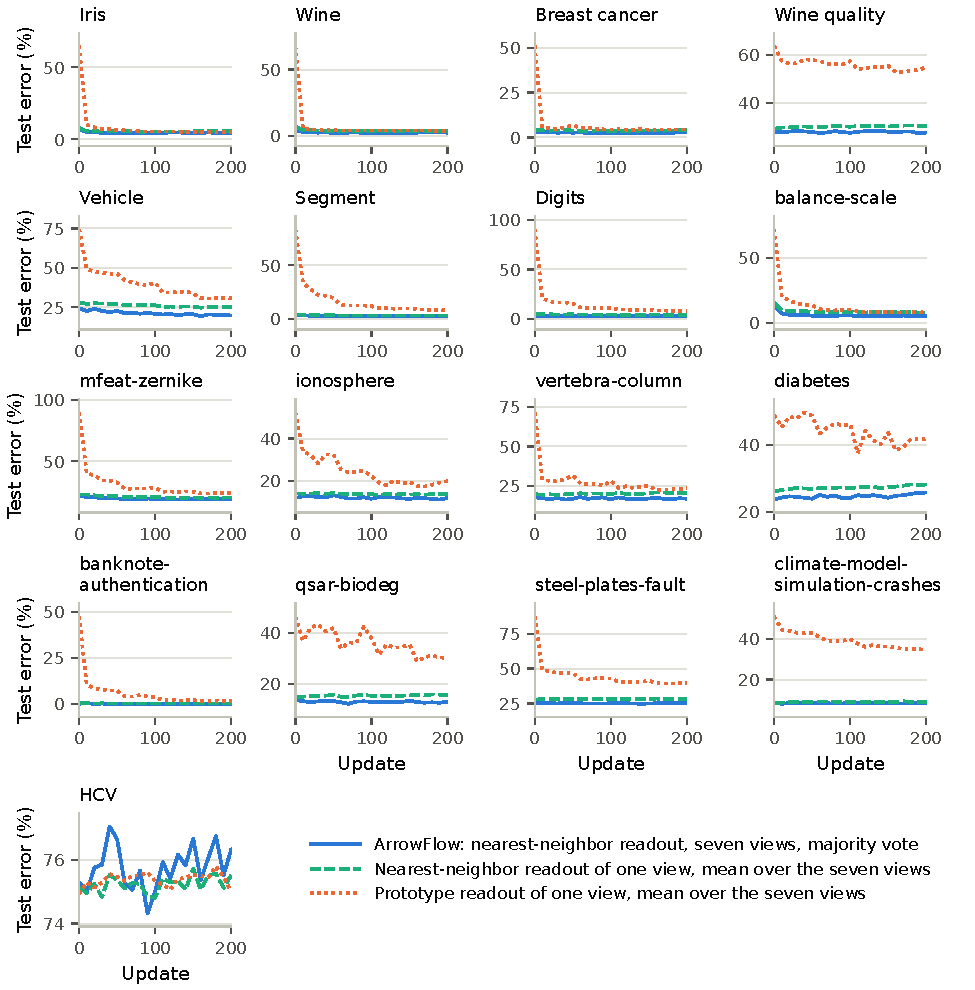
\includegraphics[width=\textwidth]{figures/data/figS_learning_curves.pdf}
\caption{\textbf{Training diagnostics: learning curves.} Test error in percent on the outer test rows against the number of updates, every ten updates from the initial filters, update 0, to update 200, for one fitting seed; each point is the mean over the 15 outer folds. Solid: ArrowFlow's seven-view nearest-neighbor readout, combined by majority vote. Dashed: the nearest-neighbor readout of one view, and dotted: the prototype readout of one view, each averaged over the seven views. The curves follow the filters through training, while the network that ArrowFlow returns is the one at its checkpoint (Table~\ref{tab:s-diag-checkpoints}). Each panel has its own error scale. Descriptive: nothing is selected or tested. At update 200 the prototype readout of one view has higher test error than the nearest-neighbor readout of one view on 15 of the 17 datasets. HCV: hepatitis C virus.}
\label{fig:learning-curves}
\end{figure}


Post hoc and descriptively, these diagnostics and the component ablation suggest three reasons why the training gain is modest. First, the prototype readout drives the gate, the returned signal and the checkpoint. Yet it has higher error than even the untrained networks read by nearest neighbors on 11 of the 17 datasets (Table~\ref{tab:s-components-errors}). Its advantage over those networks tracks ArrowFlow's gain over them, with a Spearman correlation of 0.50 over the 17 datasets. Second, on Iris, Wine, Breast cancer and banknote-authentication only 1.9 to 5.3 percent of the selected slots carry a vote, against at least 10.0 percent on every other dataset (Table~\ref{tab:s-motion-statistics}). So training there has little to work with. Third, on Vehicle, Segment, Digits, mfeat-zernike and steel-plates-fault the median checkpoint is update 131 to 146 of 200, so at least half of the views there still improved their validation error after update 130 (Table~\ref{tab:s-diag-checkpoints}).

\paragraph{Does a second hidden layer help?} Two families ask whether a second hidden layer earns its place, holding everything else at the configuration the fold itself selected. It did not help in either family. The first, the fixed-configuration depth family, ran with the earlier relay. The second repeats its primary contrast with the corrected relay of Section~\ref{sec:training}.

The first family holds fixed the fold, the encoder settings, the learning rate, the iteration count and the readout. It varies the hidden widths and, in two further arms, how much of the stack is trained. Table~\ref{tab:s-depth-contrasts} gives the three contrasts, each Holm-adjusted across the seventeen datasets. The primary contrast sets one trained hidden layer against two trained hidden layers. The other two arms are weakened on purpose. The untrained-second arm adds a second hidden layer and never trains it, and the first-only arm trains the first hidden layer only.

Table~\ref{tab:s-depth-movement} gives, for each arm, the share of its hidden filters that a batch update reorders, and it must be read beside Table~\ref{tab:s-depth-contrasts}. This is a rate per update over the whole fit. It differs from the displacement of Table~\ref{tab:s-diag-displacement}, which compares each filter's initial and checkpointed orders once. So a filter that few updates reorder can still end far from where it began. Freezing the second layer also quiets the first. As a result, part of a weakened arm's deficit comes from less adaptation, and the extra layer does not explain all of it. Pooled over all folds, both fully trained depths reorder a similar share of their hidden filters per update, the two-layer networks at least nine tenths as many as the one-layer networks, although the ratio varies by dataset. One hidden layer is more accurate than the untrained-second arm on 15 of the 17 datasets, but that arm reorders less than a third as many filters as the fully trained two-layer arm. Table~\ref{tab:s-depth-subsets} repeats the primary contrast on the folds that selected one hidden layer and on those that selected two.

The second family, depth with the corrected relay, reuses the one-layer arm and the two-layer arm with the earlier relay of the first family. As a check, a refit of the first outer fold of every dataset reproduced both exactly. The family fits two new two-layer arms on the same folds, seed and settings: one with the corrected relay, and one whose first-layer votes are also multiplied by 8. The scale tests a second reason why the first layer may learn little. Its votes may be too weak to overcome the prior, the identity term of the accumulator that votes for the filter's current order. Equation~\eqref{eq:signal} keeps a relayed signal below $cV_\ell$, so a first-layer vote stays below $2\eta c$. After every batch reset, the prior dictates a filter's order while its batch vote mass stays below $1/(e-1)$ (Section~\ref{supp:iia}). The scale 8 is the smallest of 1, 2, 4, 8, 16 and 32 at which at least half of the first layer's voted filter-batches reach that threshold, on training-only pilot fits of Iris and ionosphere. The protocol fixed the reading in advance. By its rule, a corrected arm helps only if it is ahead of one hidden layer on at least 9 of the 17 datasets and significantly ahead, after Holm adjustment, on at least one.

Neither corrected arm helps (Table~\ref{tab:s-relay-contrasts}). One hidden layer is more accurate than two with the corrected relay on 9 of the 17 datasets, by $+0.24$ points on average, and than the scaled arm on 14. No contrast of either arm survives Holm adjustment. The correction itself makes two-layer networks more accurate than the earlier relay on 12 of the 17 datasets, by $+0.64$ points on average, again with no Holm-significant contrast. The scaled votes reorder the first layer's filters far more often, in 81.6 against 34.5 percent of the updates on average, without making two layers more accurate (Table~\ref{tab:s-relay-movement}).

Both families run one fitting seed per fold and retune neither the learning rate nor the iteration count. So they show whether the second layer earns its place at the selected configuration. The best model attainable at either depth is a separate question, and the families say nothing about deeper stacks.

\clearpage
% Rendered by render_tables.py from run files; do not edit by hand.
\begin{table}[!htbp]
\caption{\textbf{Depth at a matched configuration.} One hidden layer minus each two-layer arm, accuracy, in percentage points with the 95\% corrected resampled-$t$ interval (test-to-training ratio 0.25, 14 degrees of freedom); positive favors one layer. Every arm reads the same per-fold selection, the same splits and one fitting seed, and neither the learning rate nor the update count is retuned. The untrained-second arm never moves its second hidden layer; the first-only arm never moves the layer the readout reads. Every two-layer arm used the earlier relay of Section~\ref{sec:training}; Table~\ref{tab:s-relay-contrasts} repeats the primary contrast with the corrected relay. Holm adjusts across the seventeen datasets within each arm. One hidden layer is more accurate than two on 15 of the 17 datasets at a matched configuration, none of the seventeen contrasts survives Holm adjustment, and the largest difference is mfeat-zernike +2.98 points (Holm 0.056). HCV: hepatitis C virus.}
\label{tab:s-depth-contrasts}
\centering
\scriptsize
\setlength{\tabcolsep}{3pt}
\resizebox{\ifdim\width>\linewidth\linewidth\else\width\fi}{!}{%
\begin{tabular}{lrrrrrr}
\toprule
Dataset & \begin{tabular}[b]{@{}r@{}}Two\\Diff. (pp) [interval]\end{tabular} & \begin{tabular}[b]{@{}r@{}}Two\\Holm $p$\end{tabular} & \begin{tabular}[b]{@{}r@{}}Untrained\\Diff. (pp) [interval]\end{tabular} & \begin{tabular}[b]{@{}r@{}}Untrained\\Holm $p$\end{tabular} & \begin{tabular}[b]{@{}r@{}}First\\Diff. (pp) [interval]\end{tabular} & \begin{tabular}[b]{@{}r@{}}First\\Holm $p$\end{tabular} \\
\midrule
Iris & +0.44 [$-$1.63, +2.52] & 1.000 & +1.33 [$-$2.00, +4.66] & 1.000 & +0.22 [$-$1.62, +2.06] & 1.000 \\
Wine & +0.37 [$-$1.80, +2.54] & 1.000 & +1.49 [$-$2.13, +5.12] & 1.000 & +0.17 [$-$3.58, +3.93] & 1.000 \\
Breast cancer & $-$0.29 [$-$1.78, +1.19] & 1.000 & +0.47 [$-$1.53, +2.46] & 1.000 & +0.70 [$-$1.27, +2.67] & 1.000 \\
Wine quality & +0.77 [$-$1.27, +2.81] & 1.000 & +0.54 [$-$1.46, +2.55] & 1.000 & +0.25 [$-$1.02, +1.52] & 1.000 \\
Vehicle & +2.96 [$-$0.51, +6.42] & 1.000 & +4.02 [$-$0.07, +8.10] & 0.697 & +4.89 [+1.97, +7.81] & 0.044 \\
Segment & +1.15 [+0.01, +2.30] & 0.717 & +1.18 [+0.06, +2.31] & 0.569 & +0.92 [$-$0.02, +1.87] & 0.764 \\
Digits & +0.63 [$-$0.60, +1.86] & 1.000 & +1.22 [+0.18, +2.27] & 0.373 & +1.21 [$-$0.07, +2.48] & 0.818 \\
balance-scale & +1.65 [+0.17, +3.13] & 0.499 & +7.04 [+4.40, +9.68] & $<$0.001 & +6.03 [+2.57, +9.49] & 0.035 \\
mfeat-zernike & +2.98 [+1.17, +4.79] & 0.056 & +6.33 [+4.59, +8.08] & $<$0.001 & +4.28 [+2.73, +5.84] & $<$0.001 \\
ionosphere & +1.05 [$-$2.24, +4.33] & 1.000 & +0.76 [$-$2.73, +4.24] & 1.000 & +1.42 [$-$1.69, +4.54] & 1.000 \\
vertebra-column & +0.22 [$-$3.60, +4.03] & 1.000 & +1.51 [$-$3.67, +6.68] & 1.000 & +0.11 [$-$3.05, +3.27] & 1.000 \\
diabetes & +1.87 [$-$0.39, +4.12] & 1.000 & +1.09 [$-$1.92, +4.09] & 1.000 & +1.22 [$-$1.55, +3.98] & 1.000 \\
banknote-authentication & +0.00 [$-$0.23, +0.24] & 1.000 & $-$0.10 [$-$0.71, +0.51] & 1.000 & $-$0.12 [$-$0.71, +0.47] & 1.000 \\
qsar-biodeg & +1.01 [$-$1.26, +3.28] & 1.000 & +1.42 [$-$1.36, +4.20] & 1.000 & +1.33 [$-$1.16, +3.81] & 1.000 \\
steel-plates-fault & +1.53 [$-$0.13, +3.19] & 0.957 & +1.39 [$-$0.17, +2.95] & 0.922 & +1.12 [$-$0.82, +3.06] & 1.000 \\
climate-model-simulation-crashes & +0.12 [$-$0.45, +0.70] & 1.000 & +0.19 [$-$0.28, +0.65] & 1.000 & +0.19 [$-$0.28, +0.65] & 1.000 \\
HCV & $-$1.44 [$-$5.18, +2.30] & 1.000 & $-$0.26 [$-$3.36, +2.83] & 1.000 & $-$0.94 [$-$4.53, +2.65] & 1.000 \\
\bottomrule
\end{tabular}
}
\end{table}

% Rendered by render_tables.py from run files; do not edit by hand.
\begin{table}[!htbp]
\caption{\textbf{Depth: how much each arm moved.} Share of the hidden filter updates that change the filter's order, in percent. Every batch updates each hidden filter once, and the share pools the batches, the hidden layers and the seven views of a fit and is averaged over the outer folds. It is a rate per update, not the displacement at the checkpoint of Table~\ref{tab:s-diag-displacement}. The last columns count the outer folds on which an arm is effectively inert, that is below a changed share of 0.01. The last row pools all 255 folds. A contrast against an arm that barely moves is evidence about movement, not about depth. Descriptive. Over all folds a hidden filter update reorders the filter in 67.8 and 63.8 percent of the cases in the two fully trained arms, in 13.3 percent in the untrained-second arm and in 18.4 percent in the first-only arm. HCV: hepatitis C virus.}
\label{tab:s-depth-movement}
\centering
\scriptsize
\setlength{\tabcolsep}{3pt}
\resizebox{\ifdim\width>\linewidth\linewidth\else\width\fi}{!}{%
\begin{tabular}{lrrrrrrr}
\toprule
Dataset & \begin{tabular}[b]{@{}r@{}}One\\changed (\%)\end{tabular} & \begin{tabular}[b]{@{}r@{}}Two\\changed (\%)\end{tabular} & \begin{tabular}[b]{@{}r@{}}Untrained\\changed (\%)\end{tabular} & \begin{tabular}[b]{@{}r@{}}First\\changed (\%)\end{tabular} & \begin{tabular}[b]{@{}r@{}}Two\\inert folds\end{tabular} & \begin{tabular}[b]{@{}r@{}}Untrained\\inert folds\end{tabular} & \begin{tabular}[b]{@{}r@{}}First\\inert folds\end{tabular} \\
\midrule
Iris & 11.6 & 18.0 & 0.9 & 5.9 & 0 & 4 & 0 \\
Wine & 16.0 & 14.3 & 3.2 & 20.3 & 0 & 0 & 0 \\
Breast cancer & 33.4 & 28.6 & 3.1 & 15.4 & 0 & 5 & 0 \\
Wine quality & 99.5 & 86.9 & 17.3 & 19.3 & 0 & 0 & 0 \\
Vehicle & 80.9 & 69.9 & 10.0 & 14.2 & 0 & 0 & 0 \\
Segment & 77.5 & 83.2 & 21.5 & 28.6 & 0 & 0 & 0 \\
Digits & 70.7 & 77.5 & 27.9 & 31.5 & 0 & 0 & 0 \\
balance-scale & 60.9 & 54.4 & 4.9 & 12.9 & 0 & 0 & 0 \\
mfeat-zernike & 97.3 & 89.7 & 29.1 & 31.1 & 0 & 0 & 0 \\
ionosphere & 63.7 & 74.5 & 19.0 & 25.2 & 0 & 0 & 0 \\
vertebra-column & 36.5 & 47.9 & 0.8 & 2.8 & 0 & 9 & 0 \\
diabetes & 90.9 & 73.3 & 4.2 & 5.1 & 0 & 3 & 3 \\
banknote-authentication & 18.5 & 22.4 & 0.7 & 5.7 & 0 & 4 & 0 \\
qsar-biodeg & 98.3 & 92.5 & 26.8 & 29.8 & 0 & 0 & 0 \\
steel-plates-fault & 97.9 & 86.5 & 19.2 & 23.0 & 0 & 0 & 0 \\
climate-model-simulation-crashes & 98.4 & 80.0 & 16.5 & 20.2 & 0 & 0 & 0 \\
HCV & 100.0 & 85.4 & 21.5 & 22.3 & 0 & 0 & 0 \\
\midrule
All seventeen together & 67.8 & 63.8 & 13.3 & 18.4 & 0 & 25 & 3 \\
\bottomrule
\end{tabular}
}
\end{table}

% Rendered by render_tables.py from run files; do not edit by hand.
\begin{table}[!htbp]
\caption{\textbf{Depth: the same contrast on the folds each selection chose.} One hidden layer minus two, accuracy, in percentage points, restricted to the outer folds whose own reconstructed selection was one hidden layer and to those whose selection was two. The fold sets differ by dataset and are chosen by the selection itself, so these columns describe where each architecture was selected and carry no test. Intervals are 95\% corrected resampled-$t$ intervals over the $n$ folds of a row, with the variance of the fold differences multiplied by $1/n+0.25$ and $n-1$ degrees of freedom; $n$ is the number of folds of the row's column. The fold's own selection chose two hidden layers on 70 of the 255 outer folds, and on none of the fifteen on 7 of the 17 datasets. HCV: hepatitis C virus.}
\label{tab:s-depth-subsets}
\centering
\scriptsize
\setlength{\tabcolsep}{3pt}
\resizebox{\ifdim\width>\linewidth\linewidth\else\width\fi}{!}{%
\begin{tabular}{lrrrrr}
\toprule
Dataset & \begin{tabular}[b]{@{}r@{}}Two-layer\\folds\end{tabular} & \begin{tabular}[b]{@{}r@{}}[128]\\Diff. (pp)\end{tabular} & \begin{tabular}[b]{@{}r@{}}[64,128]\\Diff. (pp)\end{tabular} & \begin{tabular}[b]{@{}r@{}}[128]\\95\% interval\end{tabular} & \begin{tabular}[b]{@{}r@{}}[64,128]\\95\% interval\end{tabular} \\
\midrule
Iris & 7 of 15 & $-$0.42 & +1.43 & [$-$2.12, +1.29] & [$-$1.30, +4.16] \\
Wine & 11 of 15 & $-$0.02 & +0.51 & [$-$5.20, +5.16] & [$-$1.68, +2.71] \\
Breast cancer & 4 of 15 & $-$0.24 & $-$0.44 & [$-$1.95, +1.46] & [$-$2.99, +2.11] \\
Wine quality & 0 of 15 & +0.77 & -- & [$-$1.27, +2.81] & -- \\
Vehicle & 3 of 15 & +3.20 & +1.97 & [$-$0.77, +7.17] & [$-$2.93, +6.86] \\
Segment & 0 of 15 & +1.15 & -- & [+0.01, +2.30] & -- \\
Digits & 0 of 15 & +0.63 & -- & [$-$0.60, +1.86] & -- \\
balance-scale & 0 of 15 & +1.65 & -- & [+0.17, +3.13] & -- \\
mfeat-zernike & 0 of 15 & +2.98 & -- & [+1.17, +4.79] & -- \\
ionosphere & 4 of 15 & +0.78 & +1.79 & [$-$2.78, +4.34] & [$-$4.84, +8.41] \\
vertebra-column & 11 of 15 & +0.00 & +0.29 & [$-$5.13, +5.13] & [$-$4.29, +4.87] \\
diabetes & 5 of 15 & +1.69 & +2.22 & [$-$0.63, +4.02] & [$-$2.03, +6.46] \\
banknote-authentication & 9 of 15 & $-$0.06 & +0.04 & [$-$0.31, +0.19] & [$-$0.26, +0.34] \\
qsar-biodeg & 0 of 15 & +1.01 & -- & [$-$1.26, +3.28] & -- \\
steel-plates-fault & 0 of 15 & +1.53 & -- & [$-$0.13, +3.19] & -- \\
climate-model-simulation-crashes & 5 of 15 & +0.09 & +0.19 & [$-$0.61, +0.80] & [$-$0.59, +0.96] \\
HCV & 11 of 15 & $-$3.16 & $-$0.82 & [$-$8.92, +2.60] & [$-$4.91, +3.27] \\
\bottomrule
\end{tabular}
}
\end{table}

% Rendered by render_tables.py from run files; do not edit by hand.
\begin{table}[!htbp]
\caption{\textbf{Depth with the corrected relay.} One hidden layer minus two hidden layers with the corrected relay (corrected), and minus two hidden layers whose first-layer votes are also multiplied by 8 (scaled); then two hidden layers with the corrected relay minus two with the earlier relay. Accuracy, in percentage points, with the 95\% corrected resampled-$t$ interval (test-to-training ratio 0.25, 14 degrees of freedom); positive favors the first-named. The four arms share each fold's selected configuration, splits and one fitting seed; the one-layer arm and the arm with the earlier relay are those of Table~\ref{tab:s-depth-contrasts}. Holm adjusts across the seventeen datasets within each contrast. One hidden layer is more accurate than two on 9 of the 17 datasets with the corrected relay, by +0.24 points on average, and on 14 with the scaled votes; the correction makes two-layer networks more accurate on 12, by +0.64 points on average. No contrast survives Holm adjustment. HCV: hepatitis C virus.}
\label{tab:s-relay-contrasts}
\centering
\scriptsize
\setlength{\tabcolsep}{3pt}
\resizebox{\ifdim\width>\linewidth\linewidth\else\width\fi}{!}{%
\begin{tabular}{lrrrrrr}
\toprule
Dataset & \begin{tabular}[b]{@{}r@{}}One $-$ corrected\\Diff. (pp) [interval]\end{tabular} & \begin{tabular}[b]{@{}r@{}}One $-$ corrected\\Holm $p$\end{tabular} & \begin{tabular}[b]{@{}r@{}}One $-$ scaled\\Diff. (pp) [interval]\end{tabular} & \begin{tabular}[b]{@{}r@{}}One $-$ scaled\\Holm $p$\end{tabular} & \begin{tabular}[b]{@{}r@{}}Corrected $-$ earlier\\Diff. (pp) [interval]\end{tabular} & \begin{tabular}[b]{@{}r@{}}Corrected $-$ earlier\\Holm $p$\end{tabular} \\
\midrule
Iris & +0.00 [$-$2.15, +2.15] & 1.000 & +0.67 [$-$2.05, +3.39] & 1.000 & +0.44 [$-$2.13, +3.02] & 1.000 \\
Wine & $-$0.75 [$-$3.13, +1.64] & 1.000 & $-$0.01 [$-$2.23, +2.21] & 1.000 & +1.12 [$-$1.96, +4.19] & 1.000 \\
Breast cancer & $-$0.06 [$-$1.30, +1.18] & 1.000 & +0.06 [$-$1.47, +1.59] & 1.000 & $-$0.23 [$-$2.13, +1.66] & 1.000 \\
Wine quality & +1.40 [$-$0.69, +3.48] & 1.000 & +0.39 [$-$2.13, +2.92] & 1.000 & $-$0.63 [$-$2.92, +1.66] & 1.000 \\
Vehicle & $-$0.39 [$-$2.40, +1.62] & 1.000 & +3.51 [+0.50, +6.51] & 0.434 & +3.35 [$-$0.34, +7.03] & 1.000 \\
Segment & +0.45 [$-$0.19, +1.08] & 1.000 & +0.20 [$-$0.58, +0.98] & 1.000 & +0.71 [$-$0.66, +2.08] & 1.000 \\
Digits & +0.69 [$-$0.23, +1.60] & 1.000 & +0.24 [$-$0.66, +1.15] & 1.000 & $-$0.06 [$-$1.05, +0.94] & 1.000 \\
balance-scale & +0.80 [$-$2.25, +3.85] & 1.000 & +1.01 [$-$0.51, +2.54] & 1.000 & +0.85 [$-$2.23, +3.94] & 1.000 \\
mfeat-zernike & +1.08 [$-$0.97, +3.14] & 1.000 & +1.00 [$-$0.73, +2.73] & 1.000 & +1.90 [$-$0.15, +3.95] & 1.000 \\
ionosphere & +0.85 [$-$3.64, +5.34] & 1.000 & +1.81 [$-$1.21, +4.82] & 1.000 & +0.20 [$-$4.34, +4.74] & 1.000 \\
vertebra-column & $-$0.75 [$-$5.57, +4.06] & 1.000 & +0.43 [$-$4.07, +4.93] & 1.000 & +0.97 [$-$3.25, +5.18] & 1.000 \\
diabetes & +1.22 [$-$1.52, +3.95] & 1.000 & +2.04 [$-$1.26, +5.34] & 1.000 & +0.65 [$-$1.97, +3.27] & 1.000 \\
banknote-authentication & +0.00 [$-$0.23, +0.24] & 1.000 & $-$0.07 [$-$0.32, +0.17] & 1.000 & +0.00 [+0.00, +0.00] & 1.000 \\
qsar-biodeg & $-$0.03 [$-$2.02, +1.96] & 1.000 & +1.01 [$-$1.00, +3.03] & 1.000 & +1.04 [$-$0.77, +2.85] & 1.000 \\
steel-plates-fault & +0.39 [$-$1.83, +2.62] & 1.000 & +0.26 [$-$1.84, +2.36] & 1.000 & +1.13 [$-$0.69, +2.95] & 1.000 \\
climate-model-simulation-crashes & $-$0.06 [$-$1.14, +1.01] & 1.000 & +0.06 [$-$0.60, +0.73] & 1.000 & +0.19 [$-$0.78, +1.15] & 1.000 \\
HCV & $-$0.77 [$-$4.54, +3.00] & 1.000 & $-$1.25 [$-$5.11, +2.60] & 1.000 & $-$0.67 [$-$3.45, +2.11] & 1.000 \\
\bottomrule
\end{tabular}
}
\end{table}

% Rendered by render_tables.py from run files; do not edit by hand.
\begin{table}[!htbp]
\caption{\textbf{Depth with the corrected relay: how much the first hidden layer moved.} Reordered: the share of the first hidden layer's filter updates that change the filter's order, in percent. Every batch updates each filter once, and the share pools the batches and the seven views of a fit and is averaged over the outer folds. Clearing: among the first layer's filter-batches with at least one nonzero vote, the share whose vote mass $M$ reaches the prior's threshold, $M(e-1)\ge1$, below which the prior dictates the filter's order (Section~\ref{supp:iia}); the record of the earlier relay does not hold it. Descriptive. On average over the seventeen datasets a batch update reorders 39.7, 34.5 and 81.6 percent of the first-layer filters with the earlier relay, the corrected relay and the scaled votes. The scaled votes clear the prior in 97.7 percent of the voted filter-batches, against 58.4 with the corrected relay. HCV: hepatitis C virus.}
\label{tab:s-relay-movement}
\centering
\scriptsize
\setlength{\tabcolsep}{3pt}
\begin{tabular}{lrrrrr}
\toprule
Dataset & \begin{tabular}[b]{@{}r@{}}Earlier\\reordered (\%)\end{tabular} & \begin{tabular}[b]{@{}r@{}}Corrected\\reordered (\%)\end{tabular} & \begin{tabular}[b]{@{}r@{}}Scaled\\reordered (\%)\end{tabular} & \begin{tabular}[b]{@{}r@{}}Corrected\\clearing (\%)\end{tabular} & \begin{tabular}[b]{@{}r@{}}Scaled\\clearing (\%)\end{tabular} \\
\midrule
Iris & 4.0 & 4.5 & 53.3 & 19.7 & 90.2 \\
Wine & 4.8 & 5.5 & 55.8 & 37.1 & 99.8 \\
Breast cancer & 9.5 & 8.8 & 45.4 & 33.5 & 97.2 \\
Wine quality & 61.7 & 57.1 & 97.9 & 86.8 & 99.9 \\
Vehicle & 37.6 & 28.2 & 90.7 & 57.2 & 98.5 \\
Segment & 67.8 & 45.9 & 94.6 & 68.5 & 100.0 \\
Digits & 55.7 & 46.3 & 87.4 & 70.0 & 99.9 \\
balance-scale & 17.8 & 13.0 & 81.2 & 34.9 & 97.5 \\
mfeat-zernike & 71.8 & 68.3 & 98.9 & 86.8 & 100.0 \\
ionosphere & 62.5 & 40.5 & 87.5 & 68.7 & 100.0 \\
vertebra-column & 6.8 & 6.6 & 74.1 & 18.0 & 92.3 \\
diabetes & 25.2 & 23.1 & 88.3 & 60.8 & 97.9 \\
banknote-authentication & 4.4 & 2.5 & 41.9 & 15.0 & 88.8 \\
qsar-biodeg & 84.6 & 81.4 & 96.9 & 93.2 & 100.0 \\
steel-plates-fault & 61.1 & 50.0 & 98.6 & 83.7 & 99.9 \\
climate-model-simulation-crashes & 43.7 & 42.4 & 96.0 & 71.5 & 99.9 \\
HCV & 56.1 & 61.7 & 99.3 & 87.5 & 99.9 \\
\midrule
Mean over the seventeen & 39.7 & 34.5 & 81.6 & 58.4 & 97.7 \\
\bottomrule
\end{tabular}
\end{table}


\paragraph{Does the voting rule make a difference?} This family asks whether the aggregation rule of the update changes what is learned, with everything else held at the fold's own configuration. Its answer is limited, because the median barely learned in ArrowFlow's layers. The Borda arm is the deployed rule. The median arm replaces the accumulator's squared rank distance by the footrule and solves the resulting assignment exactly. Negative votes enter it as votes for the reversed target. Under the squared distance, a vote for the reversed target acts as a vote of negative weight for the target itself (Section~\ref{supp:proofs}). The footrule has no such identity.

A plain substitution proved unusable as an aggregation comparison. With the unit prior, a prior of weight one as in the Borda count, the median barely moves the filters. So on many folds it is effectively inert, and its contrast measures movement instead of the rule (Table~\ref{tab:s-aggregation-movement}). A third arm, the prior-scaled median, therefore matches the movement by rescaling its prior. Its prior counts as four ballots of the mean incoming vote weight, where Borda's prior has weight one. The multiple was chosen on a training-only ladder over two pilot datasets as the value whose movement rate comes closest to Borda's. The ladder tried a series of candidate multiples on training data only, and the chosen value was then sealed in the protocol before the run. The two arms therefore differ in the rule and in the weight of the prior, and per dataset their movement still differs (Table~\ref{tab:s-aggregation-movement}). Table~\ref{tab:s-aggregation-contrasts} gives the one comparison that is about the aggregation rule, Borda minus the prior-scaled median, Holm-adjusted across the seventeen datasets.

The scope is narrow by design. The rules are exchanged in the hidden-layer update only, and the output layer keeps its Borda count. And the family runs one fitting seed per fold. The study is not a test of Arrow's theorem or of independence of irrelevant alternatives, and an inert arm is never read as evidence for or against a rule. It is the only measurement of the voting rule inside ArrowFlow's own layers. The laboratory of Section~\ref{supp:laboratory} compares the rules inside a permutation learning vector quantization (LVQ) layer instead. Post hoc, the prior-scaled median ends within 0.2 points of the untrained networks of Section~\ref{supp:ablation-arrowflow} on 11 of the 17 datasets. This match is only approximate, because this family fits one seed and the component ablation three. On those datasets, Borda minus the median nearly equals ArrowFlow minus the untrained networks. So the study shows that this median barely learned in ArrowFlow's layers. It does not show that the Borda count is the better rule in general. The configurations, the learning rate included, were chosen under the Borda count.

\clearpage
% Rendered by render_tables.py from run files; do not edit by hand.
\begin{table}[!htbp]
\caption{\textbf{Aggregation: Borda minus the prior-scaled median.} Accuracy difference in percentage points with the 95\% corrected resampled-$t$ interval (test-to-training ratio 0.25, 14 degrees of freedom); positive favors the Borda count. The prior-scaled median receives the same ballots as the Borda count, but its prior counts as four ballots of the mean incoming vote weight, where Borda's prior has weight one. The multiple was chosen on training-only pilot fits of two datasets so that it moved the filters about as often as Borda on those fits. The arms therefore differ in how the votes are combined and in the weight of the prior. One fitting seed and one selection per fold; Holm adjusts across the seventeen datasets. This is a comparison of two vote-combining rules and not a test of any axiom. Against the prior-scaled median, Borda is more accurate on 13 of the 17 datasets, and Vehicle +7.05 points (Holm 0.012) is the only contrast that survives Holm adjustment. HCV: hepatitis C virus.}
\label{tab:s-aggregation-contrasts}
\centering
\scriptsize
\setlength{\tabcolsep}{3pt}
\begin{tabular}{lrrrr}
\toprule
Dataset & Diff. (pp) & 95\% interval & $p$ & Holm $p$ \\
\midrule
Iris & +0.44 & [$-$2.13, +3.02] & 0.717 & 1.000 \\
Wine & +0.55 & [$-$2.08, +3.18] & 0.660 & 1.000 \\
Breast cancer & +0.64 & [$-$0.71, +2.00] & 0.325 & 1.000 \\
Wine quality & $-$0.02 & [$-$2.44, +2.40] & 0.985 & 1.000 \\
Vehicle & +7.05 & [+3.56, +10.54] & $<$0.001 & 0.012 \\
Segment & +1.10 & [+0.39, +1.81] & 0.005 & 0.081 \\
Digits & $-$0.04 & [$-$1.23, +1.16] & 0.948 & 1.000 \\
balance-scale & +4.00 & [+1.34, +6.66] & 0.006 & 0.085 \\
mfeat-zernike & +2.37 & [+0.82, +3.92] & 0.006 & 0.083 \\
ionosphere & +1.42 & [$-$2.85, +5.69] & 0.486 & 1.000 \\
vertebra-column & +1.18 & [$-$4.35, +6.71] & 0.653 & 1.000 \\
diabetes & +0.74 & [$-$1.56, +3.03] & 0.503 & 1.000 \\
banknote-authentication & $-$0.07 & [$-$0.76, +0.62] & 0.824 & 1.000 \\
qsar-biodeg & +1.14 & [$-$1.07, +3.34] & 0.287 & 1.000 \\
steel-plates-fault & +0.82 & [$-$1.13, +2.77] & 0.380 & 1.000 \\
climate-model-simulation-crashes & $-$0.06 & [$-$0.95, +0.83] & 0.884 & 1.000 \\
HCV & +0.43 & [$-$4.28, +5.14] & 0.846 & 1.000 \\
\bottomrule
\end{tabular}
\end{table}

% Rendered by render_tables.py from run files; do not edit by hand.
\begin{table}[!htbp]
\caption{\textbf{Aggregation: how much each rule moved.} Share of the hidden filter updates that change the filter's order, in percent, as in Table~\ref{tab:s-depth-movement}: a rate per batch update, averaged over the outer folds. The last columns count the outer folds on which the rule is effectively inert, that is below a changed share of 0.01. The last row pools all 255 folds. The plain median is effectively inert on 127 of the 255 folds, with a mean changed share of 0.039 against 0.671 for Borda, so its contrast measures movement and not the aggregation rule. HCV: hepatitis C virus.}
\label{tab:s-aggregation-movement}
\centering
\scriptsize
\setlength{\tabcolsep}{3pt}
\resizebox{\ifdim\width>\linewidth\linewidth\else\width\fi}{!}{%
\begin{tabular}{lrrrrr}
\toprule
Dataset & \begin{tabular}[b]{@{}r@{}}Borda\\changed (\%)\end{tabular} & \begin{tabular}[b]{@{}r@{}}Plain\\changed (\%)\end{tabular} & \begin{tabular}[b]{@{}r@{}}Prior-scaled\\changed (\%)\end{tabular} & \begin{tabular}[b]{@{}r@{}}Plain\\inert folds\end{tabular} & \begin{tabular}[b]{@{}r@{}}Prior-scaled\\inert folds\end{tabular} \\
\midrule
Iris & 14.9 & 0.9 & 35.7 & 8 of 15 & 0 of 15 \\
Wine & 14.5 & 0.4 & 5.7 & 15 of 15 & 0 of 15 \\
Breast cancer & 31.4 & 0.4 & 2.2 & 15 of 15 & 7 of 15 \\
Wine quality & 99.5 & 8.9 & 88.0 & 1 of 15 & 0 of 15 \\
Vehicle & 78.0 & 10.1 & 85.4 & 3 of 15 & 0 of 15 \\
Segment & 77.5 & 2.8 & 68.4 & 5 of 15 & 0 of 15 \\
Digits & 70.7 & 1.1 & 8.3 & 10 of 15 & 0 of 15 \\
balance-scale & 60.9 & 2.2 & 19.4 & 5 of 15 & 0 of 15 \\
mfeat-zernike & 97.3 & 1.0 & 88.2 & 6 of 15 & 0 of 15 \\
ionosphere & 67.2 & 4.7 & 49.6 & 9 of 15 & 0 of 15 \\
vertebra-column & 44.7 & 0.8 & 65.2 & 11 of 15 & 0 of 15 \\
diabetes & 85.1 & 9.1 & 66.9 & 6 of 15 & 0 of 15 \\
banknote-authentication & 21.9 & 1.2 & 30.8 & 8 of 15 & 0 of 15 \\
qsar-biodeg & 98.3 & 6.4 & 70.9 & 8 of 15 & 0 of 15 \\
steel-plates-fault & 97.9 & 2.6 & 91.2 & 6 of 15 & 0 of 15 \\
climate-model-simulation-crashes & 91.3 & 3.8 & 74.5 & 11 of 15 & 0 of 15 \\
HCV & 89.3 & 9.3 & 96.3 & 0 of 15 & 0 of 15 \\
\midrule
All seventeen together & 67.1 & 3.9 & 55.7 & 127 of 255 & 7 of 255 \\
\bottomrule
\end{tabular}
}
\end{table}


\paragraph{Do established methods do as well?} These four models ask whether established neighborhood learning reaches ArrowFlow's accuracy on the same rows. One of them, a kernel method on rankings, is more accurate than ArrowFlow on 14 of the 17 datasets. Three of them are a numeric nearest-neighbor classifier after a projection:
\begin{itemize}[leftmargin=2em,topsep=2pt,itemsep=1pt]
\item linear discriminant analysis (LDA), which uses the labels;
\item principal component analysis (PCA), its label-free counterpart at the same candidate settings;
\item neighborhood components analysis (NCA), which learns a metric, a way of measuring the distance between rows.
\end{itemize}
The fourth is a support vector classifier on a precomputed Kendall kernel over rankings from ArrowFlow's encoder family. The Kendall kernel of two rankings is Kendall's $\tau$. It counts the item pairs that the two rankings order the same way, subtracts the pairs they order differently and divides by the number of pairs. The classifier uses seven views, at the encoder settings and the value of $C$ that it chooses on its inner folds (Table~\ref{tab:s-grids}), and it combines them by majority vote. Its $C$ sets how strongly training errors are penalized. It therefore reads the kind of representation the ranking layers receive, though not always at ArrowFlow's settings. A software test shows that its view encoders produce arrays identical to those of the control that reads the input rankings. The angle property of Section~\ref{supp:angle} suggests why this classifier does well. For a random view, the Kendall kernel of two encoded rankings has the expected value $1-2\theta/\pi$ over the random projection, where $\theta$ is the angle between the two inputs' expanded, standardized features. This is twice the arc-cosine kernel of order 0 of \citet{cho2009kernel}, minus one. So on such views the classifier behaves much like a kernel machine on the features.

Every baseline runs under the registered nested design. The preparation stage reproduced the dataset and split hashes of the registered runs, so the contrasts are paired fold by fold. ArrowFlow itself is never refitted, and its stored predictions are reused. Table~\ref{tab:s-baseline-families} gives the four Holm families, one per baseline, each adjusted across the seventeen datasets and the four adjusted separately. Table~\ref{tab:s-baseline-intervals} gives their intervals and unadjusted $p$ values. The intervals are not simultaneous, so each holds for its own contrast without allowance for the others. Table~\ref{tab:s-baseline-errors} gives mean outer-fold error, and Table~\ref{tab:s-baseline-ranks} the rank panel over all eleven models. Table~\ref{tab:s-baseline-warnings} lists the convergence warnings. NCA stands for supervised metric learning here. Large-margin nearest neighbor (LMNN) learning \citep{weinberger2009lmnn}, another method of this kind, was not run.

These baselines test the alternative explanation by comparison alone. They show whether established methods on the same rows, and a fixed permutation kernel on rankings from the same encoder family, reach the deployed readout's accuracy. They do not separate the filter update from the encoder. That separation is the work of the training controls of Section~\ref{supp:training} and the component ablation of Section~\ref{supp:ablations}.

\clearpage
% Rendered by render_tables.py from run files; do not edit by hand.
\begin{table}[!htbp]
\caption{\textbf{Neighbor baselines: the four Holm families.} ArrowFlow minus the baseline, accuracy, in percentage points; positive favors ArrowFlow. Every contrast is paired: the same rows, the same outer folds and the same fitting seeds as the registered runs, whose ArrowFlow predictions are reused and not refitted. Holm adjusts across the seventeen datasets within each baseline, the four baselines separately. LDA: linear discriminant analysis; PCA: principal component analysis; NCA: neighborhood components analysis. The Kendall SVC is a support vector classifier with a fixed Kendall kernel on rankings from ArrowFlow's encoder family, at encoder settings it chooses on its own inner folds. A fixed Kendall kernel on rankings from the same encoder family has a higher mean accuracy than ArrowFlow on 14 of the 17 datasets, with a mean difference of $-$0.77 points. ArrowFlow has the higher mean accuracy on 12 of the 17 against LDA kNN, 11 of the 17 against PCA kNN, 7 of the 17 against NCA kNN. HCV: hepatitis C virus.}
\label{tab:s-baseline-families}
\centering
\scriptsize
\setlength{\tabcolsep}{3pt}
\resizebox{\ifdim\width>\linewidth\linewidth\else\width\fi}{!}{%
\begin{tabular}{lrrrr}
\toprule
Dataset & \begin{tabular}[b]{@{}r@{}}LDA kNN\\Diff. (pp)\end{tabular} & \begin{tabular}[b]{@{}r@{}}PCA kNN\\Diff. (pp)\end{tabular} & \begin{tabular}[b]{@{}r@{}}NCA kNN\\Diff. (pp)\end{tabular} & \begin{tabular}[b]{@{}r@{}}Kendall SVC\\Diff. (pp)\end{tabular} \\
\midrule
Iris & $-$2.37 & $-$0.37 & $-$1.48 & $-$0.44 \\
Wine & $-$1.87 & $-$0.37 & $-$0.56 & $-$0.74 \\
Breast cancer & +1.48 & +1.48 & +0.66 & $-$0.20 \\
Wine quality & +2.29 & +0.94 & +1.25 & +1.15 \\
Vehicle & +2.15 & +8.02 & +4.68 & $-$1.80 \\
Segment & +0.03 & +1.31 & +0.58 & +0.02 \\
Digits & +0.57 & $-$0.39 & $-$0.50 & $-$0.88 \\
balance-scale & +3.57 & +3.89 & $-$1.60 & $-$0.89 \\
mfeat-zernike & $-$1.43 & $-$0.14 & $-$0.04 & $-$0.53 \\
ionosphere & +2.27 & +2.37 & +1.53 & $-$1.52 \\
vertebra-column & +2.69 & +3.66 & $-$0.11 & $-$1.11 \\
diabetes & +0.35 & +0.21 & +0.74 & +0.09 \\
banknote-authentication & +0.45 & +0.13 & $-$0.14 & $-$0.18 \\
qsar-biodeg & +1.50 & +2.22 & +2.63 & $-$0.59 \\
steel-plates-fault & +2.86 & +1.29 & $-$0.77 & $-$1.38 \\
climate-model-simulation-crashes & $-$3.70 & $-$1.42 & $-$2.53 & $-$3.15 \\
HCV & $-$1.50 & $-$0.66 & $-$1.24 & $-$0.93 \\
\bottomrule
\end{tabular}
}
\par\medskip
\resizebox{\ifdim\width>\linewidth\linewidth\else\width\fi}{!}{%
\begin{tabular}{lrrrr}
\toprule
Dataset & \begin{tabular}[b]{@{}r@{}}LDA kNN\\Holm $p$\end{tabular} & \begin{tabular}[b]{@{}r@{}}PCA kNN\\Holm $p$\end{tabular} & \begin{tabular}[b]{@{}r@{}}NCA kNN\\Holm $p$\end{tabular} & \begin{tabular}[b]{@{}r@{}}Kendall SVC\\Holm $p$\end{tabular} \\
\midrule
Iris & 1.000 & 1.000 & 1.000 & 1.000 \\
Wine & 1.000 & 1.000 & 1.000 & 1.000 \\
Breast cancer & 0.987 & 1.000 & 1.000 & 1.000 \\
Wine quality & 0.947 & 1.000 & 1.000 & 1.000 \\
Vehicle & 1.000 & 0.021 & 0.669 & 0.873 \\
Segment & 1.000 & 0.184 & 1.000 & 1.000 \\
Digits & 1.000 & 1.000 & 1.000 & 0.248 \\
balance-scale & 0.067 & 0.002 & 1.000 & 0.504 \\
mfeat-zernike & 1.000 & 1.000 & 1.000 & 1.000 \\
ionosphere & 1.000 & 1.000 & 1.000 & 1.000 \\
vertebra-column & 1.000 & 1.000 & 1.000 & 1.000 \\
diabetes & 1.000 & 1.000 & 1.000 & 1.000 \\
banknote-authentication & 1.000 & 1.000 & 1.000 & 1.000 \\
qsar-biodeg & 1.000 & 0.729 & 0.146 & 1.000 \\
steel-plates-fault & 0.018 & 1.000 & 1.000 & 0.248 \\
climate-model-simulation-crashes & 0.065 & 0.729 & 0.043 & 0.007 \\
HCV & 1.000 & 1.000 & 1.000 & 1.000 \\
\bottomrule
\end{tabular}
}
\end{table}

% Rendered by render_tables.py from run files; do not edit by hand.
\begin{table}[!htbp]
\caption{\textbf{Neighbor baselines: intervals and unadjusted $p$ values.} The same contrasts as the preceding table with their 95\% corrected resampled-$t$ interval (test-to-training ratio 0.25, 14 degrees of freedom) and their unadjusted $p$ values. The intervals are not simultaneous. HCV: hepatitis C virus.}
\label{tab:s-baseline-intervals}
\centering
\scriptsize
\setlength{\tabcolsep}{3pt}
\resizebox{\ifdim\width>\linewidth\linewidth\else\width\fi}{!}{%
\begin{tabular}{lrrrr}
\toprule
Dataset & \begin{tabular}[b]{@{}r@{}}LDA kNN\\95\% interval\end{tabular} & \begin{tabular}[b]{@{}r@{}}PCA kNN\\95\% interval\end{tabular} & \begin{tabular}[b]{@{}r@{}}NCA kNN\\95\% interval\end{tabular} & \begin{tabular}[b]{@{}r@{}}Kendall SVC\\95\% interval\end{tabular} \\
\midrule
Iris & [$-$6.42, +1.68] & [$-$3.52, +2.78] & [$-$5.62, +2.66] & [$-$1.86, +0.97] \\
Wine & [$-$6.04, +2.31] & [$-$2.66, +1.92] & [$-$2.30, +1.19] & [$-$3.07, +1.59] \\
Breast cancer & [$-$0.18, +3.14] & [$-$0.51, +3.48] & [$-$0.78, +2.10] & [$-$0.86, +0.47] \\
Wine quality & [$-$0.19, +4.78] & [$-$0.63, +2.50] & [$-$1.57, +4.08] & [$-$1.82, +4.13] \\
Vehicle & [$-$1.43, +5.73] & [+3.73, +12.32] & [+0.13, +9.22] & [$-$3.74, +0.15] \\
Segment & [$-$0.85, +0.91] & [+0.33, +2.29] & [$-$0.31, +1.46] & [$-$0.69, +0.74] \\
Digits & [$-$0.42, +1.56] & [$-$1.84, +1.06] & [$-$1.72, +0.71] & [$-$1.56, $-$0.19] \\
balance-scale & [+1.31, +5.84] & [+2.35, +5.44] & [$-$4.20, +1.00] & [$-$1.71, $-$0.07] \\
mfeat-zernike & [$-$3.13, +0.28] & [$-$1.43, +1.14] & [$-$1.57, +1.49] & [$-$2.25, +1.19] \\
ionosphere & [$-$0.95, +5.50] & [$-$1.28, +6.02] & [$-$2.80, +5.86] & [$-$4.66, +1.61] \\
vertebra-column & [$-$2.97, +8.35] & [$-$2.13, +9.45] & [$-$4.79, +4.58] & [$-$3.48, +1.26] \\
diabetes & [$-$2.12, +2.81] & [$-$3.26, +3.69] & [$-$2.36, +3.84] & [$-$2.33, +2.50] \\
banknote-authentication & [$-$0.55, +1.44] & [$-$0.14, +0.40] & [$-$0.73, +0.46] & [$-$0.74, +0.38] \\
qsar-biodeg & [$-$0.48, +3.47] & [$-$0.02, +4.47] & [+0.76, +4.50] & [$-$2.00, +0.82] \\
steel-plates-fault & [+1.37, +4.35] & [$-$1.13, +3.72] & [$-$2.55, +1.01] & [$-$2.46, $-$0.30] \\
climate-model-simulation-crashes & [$-$6.02, $-$1.39] & [$-$2.86, +0.02] & [$-$4.01, $-$1.05] & [$-$4.62, $-$1.68] \\
HCV & [$-$3.70, +0.70] & [$-$3.20, +1.88] & [$-$5.20, +2.73] & [$-$3.40, +1.54] \\
\bottomrule
\end{tabular}
}
\par\medskip
\resizebox{\ifdim\width>\linewidth\linewidth\else\width\fi}{!}{%
\begin{tabular}{lrrrr}
\toprule
Dataset & \begin{tabular}[b]{@{}r@{}}LDA kNN\\$p$\end{tabular} & \begin{tabular}[b]{@{}r@{}}PCA kNN\\$p$\end{tabular} & \begin{tabular}[b]{@{}r@{}}NCA kNN\\$p$\end{tabular} & \begin{tabular}[b]{@{}r@{}}Kendall SVC\\$p$\end{tabular} \\
\midrule
Iris & 0.230 & 0.805 & 0.455 & 0.512 \\
Wine & 0.354 & 0.732 & 0.503 & 0.505 \\
Breast cancer & 0.076 & 0.133 & 0.341 & 0.537 \\
Wine quality & 0.068 & 0.219 & 0.358 & 0.418 \\
Vehicle & 0.218 & 0.001 & 0.045 & 0.067 \\
Segment & 0.945 & 0.012 & 0.184 & 0.943 \\
Digits & 0.233 & 0.572 & 0.391 & 0.015 \\
balance-scale & 0.004 & $<$0.001 & 0.208 & 0.036 \\
mfeat-zernike & 0.094 & 0.813 & 0.951 & 0.521 \\
ionosphere & 0.153 & 0.185 & 0.462 & 0.315 \\
vertebra-column & 0.325 & 0.197 & 0.961 & 0.332 \\
diabetes & 0.768 & 0.896 & 0.616 & 0.940 \\
banknote-authentication & 0.353 & 0.328 & 0.627 & 0.505 \\
qsar-biodeg & 0.126 & 0.052 & 0.009 & 0.384 \\
steel-plates-fault & 0.001 & 0.271 & 0.371 & 0.016 \\
climate-model-simulation-crashes & 0.004 & 0.053 & 0.003 & $<$0.001 \\
HCV & 0.166 & 0.587 & 0.515 & 0.432 \\
\bottomrule
\end{tabular}
}
\end{table}

% Rendered by render_tables.py from run files; do not edit by hand.
\begin{table}[!htbp]
\caption{\textbf{Neighbor baselines: mean outer-fold error.} Error in percent (outer-fold SD); fitting seeds are averaged within each outer fold. The three pipelines read the imputed and scaled features with no polynomial expansion; only the Kendall SVC reads ArrowFlow's own encoder. Descriptive. HCV: hepatitis C virus.}
\label{tab:s-baseline-errors}
\centering
\scriptsize
\setlength{\tabcolsep}{3pt}
\begin{tabular}{lrrrrr}
\toprule
Dataset & ArrowFlow & LDA kNN & PCA kNN & NCA kNN & Kendall SVC \\
\midrule
Iris & 5.04 (3.51) & 2.67 (2.25) & 4.67 (2.76) & 3.56 (2.35) & 4.59 (3.36) \\
Wine & 3.18 (2.89) & 1.31 (2.09) & 2.80 (3.17) & 2.62 (2.68) & 2.43 (2.24) \\
Breast cancer & 2.68 (1.11) & 4.16 (1.54) & 4.16 (2.14) & 3.34 (1.67) & 2.48 (1.00) \\
Wine quality & 27.66 (2.06) & 29.96 (2.36) & 28.60 (1.79) & 28.91 (2.69) & 28.82 (2.72) \\
Vehicle & 19.91 (1.52) & 22.06 (2.91) & 27.93 (3.28) & 24.59 (3.00) & 18.11 (1.96) \\
Segment & 2.58 (0.67) & 2.61 (0.71) & 3.90 (1.20) & 3.16 (0.90) & 2.61 (0.78) \\
Digits & 2.78 (0.90) & 3.36 (0.80) & 2.39 (1.10) & 2.28 (0.66) & 1.90 (0.73) \\
balance-scale & 6.03 (1.34) & 9.60 (2.70) & 9.92 (1.20) & 4.43 (2.20) & 5.14 (1.66) \\
mfeat-zernike & 19.29 (1.03) & 17.87 (1.63) & 19.15 (1.34) & 19.25 (1.75) & 18.77 (1.79) \\
ionosphere & 11.21 (3.38) & 13.48 (3.56) & 13.58 (2.41) & 12.74 (4.55) & 9.68 (3.10) \\
vertebra-column & 16.88 (3.59) & 19.57 (5.17) & 20.54 (5.08) & 16.77 (4.35) & 15.77 (3.36) \\
diabetes & 24.04 (2.49) & 24.39 (2.71) & 24.26 (2.81) & 24.78 (2.74) & 24.13 (2.37) \\
banknote-authentication & 0.19 (0.46) & 0.63 (0.54) & 0.32 (0.49) & 0.05 (0.19) & 0.01 (0.03) \\
qsar-biodeg & 12.56 (1.80) & 14.06 (2.34) & 14.79 (2.64) & 15.20 (2.35) & 11.97 (2.01) \\
steel-plates-fault & 24.84 (1.55) & 27.70 (1.46) & 26.14 (1.79) & 24.08 (1.13) & 23.46 (1.50) \\
climate-model-simulation-crashes & 8.33 (0.58) & 4.63 (1.85) & 6.91 (1.15) & 5.80 (1.13) & 5.19 (1.25) \\
HCV & 75.60 (1.69) & 74.10 (2.20) & 74.95 (2.20) & 74.37 (2.85) & 74.67 (1.86) \\
\bottomrule
\end{tabular}
\end{table}

% Rendered by render_tables.py from run files; do not edit by hand.
\begin{table}[p]
\centering
\rotatebox{90}{\begin{minipage}{\textheight}
\caption{\textbf{Neighbor baselines: the rank panel.} Rank of each of the eleven models by mean outer-fold error within a dataset, 1 the lowest error; tied models share the average rank. The panel holds ArrowFlow, the five tuned comparators, the majority class and the four baselines. Descriptive: the last row is the mean rank over the datasets and carries no test. HCV: hepatitis C virus.}
\label{tab:s-baseline-ranks}
\centering
\scriptsize
\setlength{\tabcolsep}{3pt}
\resizebox{\ifdim\width>\linewidth\linewidth\else\width\fi}{!}{%
\begin{tabular}{lrrrrrrrrrrr}
\toprule
Dataset & ArrowFlow & SVC (RBF) & \begin{tabular}[b]{@{}r@{}}Random\\forest\end{tabular} & MLP & Numeric kNN & \begin{tabular}[b]{@{}r@{}}Gradient\\boosting\end{tabular} & Majority class & LDA kNN & PCA kNN & NCA kNN & Kendall SVC \\
\midrule
Iris & 8 & 3 & 9 & 4 & 6.5 & 10 & 11 & 1 & 6.5 & 2 & 5 \\
Wine & 9 & 2 & 3 & 4 & 10 & 7 & 11 & 1 & 8 & 6 & 5 \\
Breast cancer & 3 & 1 & 10 & 4 & 6 & 7 & 11 & 8 & 9 & 5 & 2 \\
Wine quality & 2 & 10 & 1 & 9 & 4 & 8 & 11 & 7 & 3 & 6 & 5 \\
Vehicle & 4 & 1 & 8 & 2 & 10 & 6 & 11 & 5 & 9 & 7 & 3 \\
Segment & 3 & 8 & 1 & 6 & 9 & 2 & 11 & 5 & 10 & 7 & 4 \\
Digits & 8 & 1 & 6 & 4 & 3 & 9 & 11 & 10 & 7 & 5 & 2 \\
balance-scale & 5 & 1 & 10 & 2 & 9 & 6 & 11 & 7 & 8 & 3 & 4 \\
mfeat-zernike & 7 & 1 & 9 & 4 & 8 & 10 & 11 & 2 & 5 & 6 & 3 \\
ionosphere & 7 & 1 & 3 & 4 & 6 & 2 & 11 & 9 & 10 & 8 & 5 \\
vertebra-column & 6 & 1 & 4 & 2 & 9 & 7 & 11 & 8 & 10 & 5 & 3 \\
diabetes & 5 & 1 & 3 & 2 & 9 & 4 & 11 & 8 & 7 & 10 & 6 \\
banknote-authentication & 5 & 3 & 10 & 1 & 6.5 & 8 & 11 & 9 & 6.5 & 4 & 2 \\
qsar-biodeg & 4 & 3 & 5 & 2 & 7 & 6 & 11 & 8 & 9 & 10 & 1 \\
steel-plates-fault & 7 & 4 & 2 & 6 & 8 & 1 & 11 & 10 & 9 & 5 & 3 \\
climate-model-simulation-crashes & 10 & 3 & 7 & 4 & 8 & 6 & 11 & 1 & 9 & 5 & 2 \\
HCV & 9 & 8 & 10 & 7 & 2.5 & 11 & 1 & 2.5 & 6 & 4 & 5 \\
\midrule
Mean rank & 6.0 & 3.1 & 5.9 & 3.9 & 7.1 & 6.5 & 10.4 & 6.0 & 7.8 & 5.8 & 3.5 \\
\bottomrule
\end{tabular}
}
\end{minipage}}
\end{table}

% Rendered by render_tables.py from run files; do not edit by hand.
\begin{table}[!htbp]
\caption{\textbf{Neighbor baselines: convergence warnings.} Fits that raised a warning, out of all fits, over the outer fits and over every fit of the complete logs, inner folds included. LDA kNN, PCA kNN and Kendall SVC raised none, so they have no column. Descriptive. Only NCA kNN raised a convergence warning: 81 of its 765 outer fits reached the iteration cap. HCV: hepatitis C virus.}
\label{tab:s-baseline-warnings}
\centering
\scriptsize
\setlength{\tabcolsep}{3pt}
\begin{tabular}{lrr}
\toprule
Dataset & \begin{tabular}[b]{@{}r@{}}NCA kNN\\outer fits\end{tabular} & \begin{tabular}[b]{@{}r@{}}NCA kNN\\all fits\end{tabular} \\
\midrule
Iris & 0 of 45 & 0 of 1215 \\
Wine & 0 of 45 & 0 of 1215 \\
Breast cancer & 0 of 45 & 0 of 1215 \\
Wine quality & 39 of 45 & 641 of 1215 \\
Vehicle & 0 of 45 & 0 of 1215 \\
Segment & 0 of 45 & 32 of 1215 \\
Digits & 0 of 45 & 0 of 1215 \\
balance-scale & 0 of 45 & 0 of 1215 \\
mfeat-zernike & 3 of 45 & 17 of 1215 \\
ionosphere & 0 of 45 & 0 of 1215 \\
vertebra-column & 0 of 45 & 16 of 1215 \\
diabetes & 12 of 45 & 90 of 1215 \\
banknote-authentication & 0 of 45 & 0 of 1215 \\
qsar-biodeg & 9 of 45 & 257 of 1215 \\
steel-plates-fault & 12 of 45 & 514 of 1215 \\
climate-model-simulation-crashes & 0 of 45 & 0 of 1215 \\
HCV & 6 of 45 & 392 of 1215 \\
\midrule
All seventeen together & 81 of 765 & 1959 of 20655 \\
\bottomrule
\end{tabular}
\end{table}


\paragraph{Does training improve the representation itself?} This family asks whether training yields a better representation or only neighborhoods that suit ArrowFlow's nearest-neighbor readout. Under a strong fixed readout, the trained rankings turned out no better than the untrained ones. The nearest-neighbor readout is tuned on the trained rankings, and training moves the filters so that an example's last hidden ranking comes nearer to the filter of its class. So a gain under the nearest-neighbor readout could come from either source. The family therefore reads three representations of every view with a strong fixed readout, a support vector classifier (SVC) on the Kendall kernel of the neighbor baselines. The three representations are the following:
\begin{itemize}[leftmargin=2em,topsep=2pt,itemsep=1pt]
\item the encoded input rankings;
\item the last hidden rankings of the untrained networks, whose filters are the trained networks' initial filters;
\item the last hidden rankings of the trained networks.
\end{itemize}
Everything runs at ArrowFlow's own per-fold selections and fitting seeds. The SVC chooses its $C$ from the grid of the Kendall SVC (Table~\ref{tab:s-grids}) on the very splits of the training rows that choose each view's nearest-neighbor readout. The seven views vote by plurality with ArrowFlow's tie rule, so the class with the most votes wins even without a majority. A refit of ArrowFlow reproduced its stored predictions on all 45 fold-seeds of every dataset. The untrained and input arms reproduced the predictions of the component ablation.

The protocol fixed the analysis and its reading before any score of these readouts existed. The primary family sets the trained against the untrained rankings under the SVC on the ten further datasets, with Holm adjustment across them. The secondary family sets the trained rankings against the encoded inputs. The paper was to state that training improves the representation itself only if two conditions hold. First, at least one primary contrast is Holm-significant in favor of the trained rankings. Second, they have the higher mean accuracy on at least 6 of the 10. Otherwise it was to state that training improves the nearest-neighbor neighborhoods but not the representation read by a strong fixed readout. The seven benchmark datasets are descriptive only, because an exploratory screen of the same question had used them before the protocol was written.

The rule is not met (Table~\ref{tab:s-rep-family}), so the second statement applies. The trained rankings have a higher mean accuracy than the untrained ones on 3 of the 10 further datasets, and the mean difference is $-0.10$ points. Against the encoded inputs they are ahead on 3 as well. No contrast of either family survives Holm adjustment. On the seven benchmark datasets the differences are below one point and of both signs. The SVC is more accurate than the nearest-neighbor readout on average on every representation, by $1.88$, $1.77$ and $0.62$ points on the input, untrained and trained rankings (Table~\ref{tab:s-rep-readouts}). Training thus closes most of the nearest-neighbor readout's gap to the SVC, while under the SVC the trained rankings are no better than the untrained ones.

\clearpage
% Rendered by render_tables.py from run files; do not edit by hand.
\begin{table}[!htbp]
\caption{\textbf{Representation test: the trained rankings under a fixed Kendall-kernel readout.} Accuracy differences, in percentage points, with the 95\% corrected resampled-$t$ interval (test-to-training ratio 0.25, 14 degrees of freedom); positive favors the trained hidden rankings. A support vector classifier on the Kendall kernel reads each representation of every view at ArrowFlow's own selected configuration and fitting seeds, and the seven views vote by plurality. The primary family is trained minus untrained rankings and the secondary family trained rankings minus the encoded input rankings, each on the ten further datasets with its own Holm adjustment. The seven benchmark datasets were screened for this question before the protocol was written, so their rows carry no $p$ value. The trained rankings have the higher mean accuracy on 3 of the 10 further datasets against the untrained rankings, with a mean difference of $-$0.10 points, and on 3 against the encoded inputs; no contrast of either family survives Holm adjustment. HCV: hepatitis C virus.}
\label{tab:s-rep-family}
\centering
\scriptsize
\setlength{\tabcolsep}{3pt}
\resizebox{\ifdim\width>\linewidth\linewidth\else\width\fi}{!}{%
\begin{tabular}{lrrrrr}
\toprule
Dataset & \begin{tabular}[b]{@{}r@{}}Trained $-$ untrained\\Diff. (pp) [interval]\end{tabular} & \begin{tabular}[b]{@{}r@{}}Trained $-$ untrained\\$p$\end{tabular} & \begin{tabular}[b]{@{}r@{}}Trained $-$ untrained\\Holm $p$\end{tabular} & \begin{tabular}[b]{@{}r@{}}Trained $-$ input\\Diff. (pp) [interval]\end{tabular} & \begin{tabular}[b]{@{}r@{}}Trained $-$ input\\Holm $p$\end{tabular} \\
\midrule
\multicolumn{6}{l}{\emph{The ten further datasets: the registered families}} \\
balance-scale & +1.10 [+0.11, +2.10] & 0.032 & 0.323 & +0.91 [$-$0.63, +2.44] & 1.000 \\
mfeat-zernike & +0.61 [$-$0.69, +1.90] & 0.332 & 1.000 & $-$0.22 [$-$1.30, +0.86] & 1.000 \\
ionosphere & $-$0.06 [$-$1.97, +1.84] & 0.945 & 1.000 & +0.19 [$-$1.82, +2.19] & 1.000 \\
vertebra-column & $-$0.11 [$-$1.31, +1.10] & 0.851 & 1.000 & $-$0.82 [$-$2.21, +0.56] & 1.000 \\
diabetes & $-$0.58 [$-$2.19, +1.03] & 0.453 & 1.000 & $-$0.71 [$-$2.19, +0.78] & 1.000 \\
banknote-authentication & $-$0.03 [$-$0.19, +0.13] & 0.672 & 1.000 & $-$0.06 [$-$0.23, +0.10] & 1.000 \\
qsar-biodeg & +0.16 [$-$0.85, +1.16] & 0.741 & 1.000 & $-$0.01 [$-$0.92, +0.90] & 1.000 \\
steel-plates-fault & $-$0.62 [$-$1.67, +0.43] & 0.228 & 1.000 & +0.23 [$-$0.99, +1.46] & 1.000 \\
climate-model-simulation-crashes & $-$1.11 [$-$2.34, +0.11] & 0.072 & 0.650 & $-$2.14 [$-$3.84, $-$0.44] & 0.175 \\
HCV & $-$0.38 [$-$1.96, +1.20] & 0.616 & 1.000 & $-$0.40 [$-$2.35, +1.55] & 1.000 \\
\midrule
\multicolumn{6}{l}{\emph{The seven benchmark datasets, screened before this protocol: descriptive}} \\
Iris & +0.37 [$-$0.72, +1.47] & -- & -- & +0.07 [$-$1.00, +1.15] & -- \\
Wine & $-$0.75 [$-$2.11, +0.61] & -- & -- & $-$0.81 [$-$2.61, +1.00] & -- \\
Breast cancer & $-$0.16 [$-$0.90, +0.59] & -- & -- & $-$0.10 [$-$0.74, +0.54] & -- \\
Wine quality & +0.10 [$-$1.65, +1.85] & -- & -- & +3.44 [$-$0.80, +7.68] & -- \\
Vehicle & +0.17 [$-$1.31, +1.66] & -- & -- & $-$0.31 [$-$2.55, +1.92] & -- \\
Segment & +0.19 [$-$0.25, +0.64] & -- & -- & +0.07 [$-$0.35, +0.49] & -- \\
Digits & $-$0.59 [$-$1.17, $-$0.01] & -- & -- & $-$0.79 [$-$1.36, $-$0.21] & -- \\
\bottomrule
\end{tabular}
}
\end{table}

% Rendered by render_tables.py from run files; do not edit by hand.
\begin{table}[!htbp]
\caption{\textbf{Representation test: the strong readout against the nearest-neighbor readout.} The Kendall-kernel support vector classifier (SVC) minus ArrowFlow's nearest-neighbor (kNN) readout on the same representation, accuracy, in percentage points; positive favors the SVC. The last column is the kNN readout of the trained minus the untrained rankings, which is ArrowFlow minus the untrained networks of Table~\ref{tab:s-components-changes}. Descriptive: no interval, no $p$ value and no adjustment. The support vector classifier is more accurate than the nearest-neighbor readout on 16, 17 and 16 of the 17 datasets on the input, untrained and trained rankings, by +1.88, +1.77 and +0.62 points on average. HCV: hepatitis C virus.}
\label{tab:s-rep-readouts}
\centering
\scriptsize
\setlength{\tabcolsep}{3pt}
\begin{tabular}{lrrrr}
\toprule
Dataset & \begin{tabular}[b]{@{}r@{}}SVC $-$ kNN,\\input (pp)\end{tabular} & \begin{tabular}[b]{@{}r@{}}SVC $-$ kNN,\\untrained (pp)\end{tabular} & \begin{tabular}[b]{@{}r@{}}SVC $-$ kNN,\\trained (pp)\end{tabular} & \begin{tabular}[b]{@{}r@{}}kNN: trained $-$\\untrained (pp)\end{tabular} \\
\midrule
Iris & +1.56 & +0.89 & +0.74 & +0.52 \\
Wine & +2.79 & +2.11 & +0.68 & +0.68 \\
Breast cancer & +0.80 & +1.09 & +0.10 & +0.84 \\
Wine quality & $-$3.20 & +0.13 & +0.21 & +0.02 \\
Vehicle & +7.17 & +5.21 & +1.77 & +3.61 \\
Segment & +1.23 & +1.19 & +0.18 & +1.20 \\
Digits & +0.87 & +0.86 & +0.12 & +0.15 \\
balance-scale & +6.04 & +5.92 & +1.67 & +5.35 \\
mfeat-zernike & +2.89 & +2.38 & +0.52 & +2.47 \\
ionosphere & +1.37 & +1.36 & +1.11 & +0.19 \\
vertebra-column & +2.87 & +1.72 & +0.97 & +0.65 \\
diabetes & +0.49 & +0.50 & +0.07 & $-$0.15 \\
banknote-authentication & +0.00 & +0.06 & +0.04 & $-$0.02 \\
qsar-biodeg & +2.14 & +1.83 & +0.73 & +1.26 \\
steel-plates-fault & +1.67 & +2.50 & +0.92 & +0.96 \\
climate-model-simulation-crashes & +2.88 & +2.12 & +0.95 & +0.06 \\
HCV & +0.34 & +0.13 & $-$0.23 & $-$0.02 \\
\midrule
Mean over the seventeen & +1.88 & +1.77 & +0.62 & +1.05 \\
\bottomrule
\end{tabular}
\end{table}


\section{Ablations}\label{supp:ablations}

This section gives the complete record of the component ablations of Section~\ref{sec:components}. To see what each part of a method contributes, an ablation removes or replaces one part at a time and keeps everything else. Each ablation evaluates its variants at the configuration that its reference method chose on the inner folds of each outer fold. An outer fold is one of the 15 test sets, and its inner folds split the rows outside it again for tuning. The reference method is ArrowFlow in the first subsection and the prototype readout in the second. The section also compares the aggregation rules that Section~\ref{sec:arrow} names at the readout and the update. An aggregation rule merges several votes or rankings into one, as the Borda count does. Unlike the ablations, the laboratory that made this comparison scored readout and update variants on inner folds only.

\FloatBarrier
\subsection{Details for Section~\ref*{sec:components}: Component Ablation of ArrowFlow}\label{supp:ablation-arrowflow}

This subsection gives the complete component ablation of Section~\ref{sec:components} on the seventeen datasets. To see what each part of ArrowFlow contributes, we remove or replace one part at a time and keep everything else. Every variant is evaluated on the same 15 outer folds and three fitting seeds at the configuration that ArrowFlow chose on the inner folds. The results are descriptive. Each difference comes with a 95\% interval but no $p$ value, and the intervals are not adjusted for the number of comparisons.

Each variant changes one part of ArrowFlow:
\begin{itemize}[leftmargin=2em,topsep=2pt,itemsep=1pt]
  \item \emph{One view} and \emph{three views} keep only part of ArrowFlow's seven views.
  \item \emph{Without checkpoint} drops the validation checkpoint, and \emph{without augmentation} drops the perturbed copies of the training rankings.
  \item The \emph{prototype readout} predicts with the nearest output filter of the same networks instead of the nearest stored training examples.
  \item The \emph{untrained networks} keep the initial filters.
  \item \emph{Footrule kNN on the same encoded inputs} reads the encoded input rankings directly and skips the ranking layers.
\end{itemize}

Table~\ref{tab:s-components-errors} gives the error of ArrowFlow and of every variant with its within-fold seed SD. This SD is the standard deviation of the error across the three fitting seeds within a fold, averaged over the folds. Table~\ref{tab:s-components-changes} gives ArrowFlow's accuracy minus the variant's with its corrected interval, a 95\% interval widened because the folds share training data (Section~\ref{supp:statistics}). We call this difference the change, and it is positive when ArrowFlow is more accurate. Table~\ref{tab:s-components-depth} gives the difference from the untrained networks by selected depth.

Some variants are read from a refit of ArrowFlow, and the others are fitted separately. The seven-view refit reproduced ArrowFlow's outer predictions exactly on all 45 fold--seed pairs of every dataset, so the variants are compared with the fitted models of Table~\ref{tab:main}. The one-view, three-view and prototype-readout variants are read from this seven-view fit. The one- and three-view variants are the first one and the first three views of that fit, so the single view is always the target-aware one. A target-aware view is one whose projection starts with coordinates fitted to separate the classes (Section~\ref{sec:encoding}). The variants without checkpoint, with untrained networks and with footrule kNN on the same encoded inputs are fitted separately. So is the variant without augmentation, but only where the adaptive rule switches augmentation on (not on Iris, Wine, Digits, mfeat-zernike, ionosphere and qsar-biodeg). The adaptive rule decides from the number of features and the number of training rows alone whether augmentation is on. Where the rule switches it off, the variant coincides with ArrowFlow. The benchmark datasets ran under protocol \texttt{arrowflow-v3-knn-ablation-1} and the further datasets under \texttt{arrowflow-v3-newdata-ablation-1}, which copies its design and takes the configuration of each outer fold from the batch run of the dataset.

% Rendered by render_tables.py from run files; do not edit by hand.
\begin{table}[!htbp]
\caption{\textbf{Error of ArrowFlow and of every variant of the component ablation.} Mean outer-fold error in percent (outer-fold SD) [mean within-fold SD across the three fitting seeds] on the seventeen datasets, every variant at the configuration that ArrowFlow chose on the inner folds of each outer fold. The seven-view refit predicted every test example as ArrowFlow did in Table~\ref{tab:main} on all 45 fold--seed pairs of every dataset, so its errors are those of ArrowFlow. n/a: the variant coincides with ArrowFlow because the adaptive rule already switches augmentation off. Descriptive. kNN: nearest-neighbor classifier; HCV: hepatitis C virus.}
\label{tab:s-components-errors}
\centering
\scriptsize
\setlength{\tabcolsep}{3pt}
\resizebox{\ifdim\width>\linewidth\linewidth\else\width\fi}{!}{%
\begin{tabular}{lrrrr}
\toprule
Dataset & \begin{tabular}[b]{@{}r@{}}ArrowFlow\\(seven views)\end{tabular} & \begin{tabular}[b]{@{}r@{}}One\\view\end{tabular} & \begin{tabular}[b]{@{}r@{}}Three\\views\end{tabular} & \begin{tabular}[b]{@{}r@{}}Without\\checkpoint\end{tabular} \\
\midrule
\multicolumn{5}{l}{\emph{Benchmark datasets}} \\
Iris & 5.0 (3.5) [1.4] & 5.0 (3.1) [2.0] & 4.9 (3.1) [1.7] & 4.5 (3.2) [0.8] \\
Wine & 3.2 (2.9) [1.6] & 4.9 (2.4) [2.5] & 3.1 (2.6) [1.8] & 2.4 (2.1) [1.1] \\
Breast cancer & 2.7 (1.1) [0.7] & 3.7 (1.4) [1.2] & 3.0 (1.3) [1.0] & 2.9 (1.3) [0.8] \\
Wine quality & 27.7 (2.1) [1.1] & 29.8 (2.0) [1.9] & 28.7 (2.0) [1.6] & 27.9 (2.1) [1.2] \\
Vehicle & 19.9 (1.5) [1.6] & 18.3 (2.1) [2.0] & 24.5 (1.9) [2.4] & 19.4 (1.8) [1.5] \\
Segment & 2.6 (0.7) [0.2] & 3.1 (0.9) [0.4] & 2.8 (0.7) [0.3] & 2.6 (0.7) [0.3] \\
Digits & 2.8 (0.9) [0.4] & 4.0 (0.9) [0.7] & 3.4 (0.9) [0.5] & 2.9 (0.9) [0.3] \\
\midrule
\multicolumn{5}{l}{\emph{Further datasets}} \\
balance-scale & 6.0 (1.3) [1.1] & 7.6 (1.6) [1.7] & 7.0 (1.9) [1.3] & 6.4 (1.5) [1.3] \\
mfeat-zernike & 19.3 (1.0) [0.9] & 19.7 (1.3) [1.3] & 19.8 (1.2) [1.1] & 19.1 (1.3) [1.0] \\
ionosphere & 11.2 (3.4) [1.9] & 12.6 (3.1) [1.8] & 12.2 (2.7) [2.2] & 11.8 (2.8) [1.8] \\
vertebra-column & 16.9 (3.6) [1.9] & 16.7 (3.3) [2.4] & 17.7 (3.3) [2.3] & 17.4 (3.5) [2.5] \\
diabetes & 24.0 (2.5) [1.3] & 25.7 (1.8) [1.8] & 25.2 (2.2) [1.6] & 25.4 (2.1) [1.8] \\
banknote-authentication & 0.2 (0.5) [0.1] & 0.2 (0.5) [0.0] & 0.2 (0.3) [0.2] & 0.1 (0.3) [0.1] \\
qsar-biodeg & 12.6 (1.8) [0.8] & 15.1 (1.8) [1.9] & 13.6 (1.9) [1.1] & 13.0 (2.0) [0.8] \\
steel-plates-fault & 24.8 (1.5) [1.0] & 27.4 (1.9) [1.4] & 26.4 (1.5) [1.1] & 25.1 (1.5) [0.9] \\
climate-model-simulation-crashes & 8.3 (0.6) [0.3] & 9.1 (1.8) [1.9] & 8.2 (0.7) [0.6] & 8.4 (0.4) [0.2] \\
HCV & 75.6 (1.7) [2.3] & 75.6 (2.0) [2.1] & 75.8 (1.8) [2.1] & 75.8 (1.7) [2.2] \\
\bottomrule
\end{tabular}
}
\par\medskip
\resizebox{\ifdim\width>\linewidth\linewidth\else\width\fi}{!}{%
\begin{tabular}{lrrrr}
\toprule
Dataset & \begin{tabular}[b]{@{}r@{}}Without\\augmentation\end{tabular} & \begin{tabular}[b]{@{}r@{}}Prototype\\readout\end{tabular} & \begin{tabular}[b]{@{}r@{}}Untrained\\networks\end{tabular} & \begin{tabular}[b]{@{}r@{}}Footrule kNN,\\same inputs\end{tabular} \\
\midrule
\multicolumn{5}{l}{\emph{Benchmark datasets}} \\
Iris & n/a & 5.8 (4.0) [2.1] & 5.6 (3.8) [1.5] & 5.9 (3.6) [0.6] \\
Wine & n/a & 3.6 (2.8) [1.8] & 3.9 (3.0) [1.5] & 4.5 (3.3) [1.5] \\
Breast cancer & 3.0 (1.1) [0.8] & 3.2 (0.9) [1.0] & 3.5 (1.3) [0.5] & 3.3 (1.2) [0.6] \\
Wine quality & 27.9 (2.3) [1.3] & 41.8 (2.0) [1.7] & 27.7 (1.9) [0.9] & 27.7 (2.0) [0.8] \\
Vehicle & 20.5 (2.0) [1.4] & 20.9 (2.1) [1.8] & 23.5 (1.9) [1.4] & 25.0 (2.0) [1.4] \\
Segment & 2.7 (0.7) [0.3] & 5.7 (0.9) [0.6] & 3.8 (1.0) [0.2] & 3.7 (1.1) [0.3] \\
Digits & n/a & 4.8 (0.9) [0.5] & 2.9 (0.9) [0.4] & 2.8 (0.9) [0.3] \\
\midrule
\multicolumn{5}{l}{\emph{Further datasets}} \\
balance-scale & 6.2 (1.5) [1.3] & 6.4 (2.3) [1.4] & 11.4 (1.5) [0.8] & 11.3 (1.4) [0.6] \\
mfeat-zernike & n/a & 19.1 (1.3) [1.3] & 21.8 (1.3) [0.9] & 21.4 (1.5) [0.6] \\
ionosphere & n/a & 11.7 (3.1) [1.8] & 11.4 (3.3) [1.3] & 11.7 (3.0) [1.2] \\
vertebra-column & 17.0 (3.2) [2.0] & 17.4 (3.8) [1.8] & 17.5 (4.0) [1.7] & 18.0 (3.5) [1.8] \\
diabetes & 24.2 (2.4) [1.2] & 26.2 (2.6) [2.2] & 23.9 (2.5) [1.4] & 23.8 (2.3) [1.5] \\
banknote-authentication & 0.1 (0.2) [0.1] & 0.3 (0.5) [0.2] & 0.2 (0.3) [0.1] & 0.1 (0.1) [0.1] \\
qsar-biodeg & n/a & 18.2 (2.1) [2.1] & 13.8 (1.8) [0.7] & 14.0 (2.0) [1.0] \\
steel-plates-fault & 24.9 (1.5) [1.0] & 30.6 (3.3) [1.3] & 25.8 (1.6) [1.0] & 25.8 (1.6) [0.8] \\
climate-model-simulation-crashes & 8.5 (0.4) [0.3] & 27.2 (4.3) [3.1] & 8.4 (0.6) [0.3] & 8.1 (0.8) [0.5] \\
HCV & 75.9 (1.8) [2.5] & 76.1 (1.5) [2.3] & 75.6 (1.6) [1.7] & 75.8 (1.7) [1.9] \\
\bottomrule
\end{tabular}
}
\end{table}

% Rendered by render_tables.py from run files; do not edit by hand.
\begin{table}[!htbp]
\caption{\textbf{ArrowFlow minus every variant, with intervals.} The differences of the component ablation of Section~\ref{sec:components} on the seventeen datasets, ArrowFlow's accuracy minus the variant's in percentage points with fitting seeds averaged within each outer fold, positive when ArrowFlow is more accurate. Each carries the 95\% corrected resampled-$t$ interval (test-to-training ratio 0.25, 14 degrees of freedom), not adjusted for multiplicity. n/a: the variant coincides with ArrowFlow because the adaptive rule already switches augmentation off. The last row averages the datasets, counting n/a as zero, and has no interval. Everything is descriptive. The benchmark datasets ran under protocol \texttt{arrowflow-v3-knn-ablation-1} and the further datasets under \texttt{arrowflow-v3-newdata-ablation-1}. kNN: nearest-neighbor classifier; HCV: hepatitis C virus.}
\label{tab:s-components-changes}
\centering
\scriptsize
\setlength{\tabcolsep}{3pt}
\resizebox{\ifdim\width>\linewidth\linewidth\else\width\fi}{!}{%
\begin{tabular}{lrrrr}
\toprule
Dataset & \begin{tabular}[b]{@{}r@{}}One\\view\end{tabular} & \begin{tabular}[b]{@{}r@{}}Three\\views\end{tabular} & \begin{tabular}[b]{@{}r@{}}Without\\checkpoint\end{tabular} & \begin{tabular}[b]{@{}r@{}}Without\\augmentation\end{tabular} \\
\midrule
\multicolumn{5}{l}{\emph{Benchmark datasets}} \\
Iris & $-$0.07 [$-$2.25, +2.10] & $-$0.15 [$-$1.89, +1.60] & $-$0.52 [$-$2.72, +1.68] & n/a \\
Wine & +1.74 [$-$0.96, +4.44] & $-$0.13 [$-$1.52, +1.27] & $-$0.74 [$-$2.34, +0.86] & n/a \\
Breast cancer & +1.01 [+0.01, +2.02] & +0.31 [$-$0.61, +1.23] & +0.27 [$-$0.56, +1.10] & +0.29 [$-$0.62, +1.21] \\
Wine quality & +2.10 [+0.40, +3.80] & +1.00 [+0.05, +1.96] & +0.21 [$-$1.46, +1.88] & +0.22 [$-$1.03, +1.47] \\
Vehicle & $-$1.60 [$-$3.84, +0.64] & +4.58 [+2.94, +6.23] & $-$0.47 [$-$2.32, +1.37] & +0.63 [$-$1.51, +2.77] \\
Segment & +0.48 [$-$0.10, +1.06] & +0.21 [$-$0.12, +0.53] & $-$0.00 [$-$0.25, +0.24] & +0.09 [$-$0.16, +0.35] \\
Digits & +1.22 [+0.70, +1.74] & +0.62 [+0.27, +0.97] & +0.12 [$-$0.31, +0.55] & n/a \\
\midrule
\multicolumn{5}{l}{\emph{Further datasets}} \\
balance-scale & +1.58 [$-$0.15, +3.31] & +0.94 [$-$0.24, +2.13] & +0.36 [$-$1.01, +1.72] & +0.14 [$-$0.95, +1.24] \\
mfeat-zernike & +0.43 [$-$0.38, +1.23] & +0.54 [+0.01, +1.07] & $-$0.14 [$-$0.79, +0.50] & n/a \\
ionosphere & +1.42 [$-$0.64, +3.48] & +0.95 [$-$0.64, +2.54] & +0.60 [$-$0.94, +2.15] & n/a \\
vertebra-column & $-$0.14 [$-$3.65, +3.36] & +0.82 [$-$1.64, +3.29] & +0.54 [$-$2.17, +3.25] & +0.11 [$-$2.02, +2.23] \\
diabetes & +1.61 [$-$0.23, +3.44] & +1.16 [$-$0.15, +2.47] & +1.32 [$-$0.53, +3.16] & +0.19 [$-$1.18, +1.55] \\
banknote-authentication & $-$0.01 [$-$0.13, +0.11] & +0.02 [$-$0.27, +0.32] & $-$0.06 [$-$0.26, +0.13] & $-$0.09 [$-$0.48, +0.30] \\
qsar-biodeg & +2.52 [+1.61, +3.42] & +0.99 [+0.14, +1.84] & +0.43 [$-$0.84, +1.70] & n/a \\
steel-plates-fault & +2.59 [+0.81, +4.38] & +1.53 [+0.49, +2.58] & +0.21 [$-$0.86, +1.28] & +0.09 [$-$0.87, +1.05] \\
climate-model-simulation-crashes & +0.78 [$-$1.17, +2.74] & $-$0.16 [$-$0.63, +0.30] & +0.10 [$-$0.26, +0.47] & +0.14 [$-$0.34, +0.63] \\
HCV & $-$0.03 [$-$2.01, +1.94] & +0.24 [$-$1.57, +2.05] & +0.18 [$-$1.38, +1.73] & +0.26 [$-$1.41, +1.92] \\
\midrule
Mean over the seventeen datasets & +0.92 & +0.79 & +0.14 & +0.12 \\
\bottomrule
\end{tabular}
}
\par\medskip
\resizebox{\ifdim\width>\linewidth\linewidth\else\width\fi}{!}{%
\begin{tabular}{lrrr}
\toprule
Dataset & \begin{tabular}[b]{@{}r@{}}Prototype\\readout\end{tabular} & \begin{tabular}[b]{@{}r@{}}Untrained\\networks\end{tabular} & \begin{tabular}[b]{@{}r@{}}Footrule kNN,\\same inputs\end{tabular} \\
\midrule
\multicolumn{4}{l}{\emph{Benchmark datasets}} \\
Iris & +0.74 [$-$1.45, +2.93] & +0.52 [$-$1.68, +2.72] & +0.89 [$-$2.28, +4.06] \\
Wine & +0.44 [$-$0.40, +1.28] & +0.68 [$-$2.06, +3.41] & +1.30 [$-$0.80, +3.40] \\
Breast cancer & +0.53 [$-$0.37, +1.42] & +0.84 [$-$0.45, +2.13] & +0.60 [$-$0.57, +1.78] \\
Wine quality & +14.15 [+11.41, +16.89] & +0.02 [$-$1.03, +1.08] & +0.03 [$-$1.07, +1.13] \\
Vehicle & +1.01 [$-$1.41, +3.43] & +3.61 [+1.18, +6.05] & +5.08 [+2.32, +7.84] \\
Segment & +3.16 [+2.17, +4.16] & +1.20 [+0.54, +1.86] & +1.12 [+0.42, +1.82] \\
Digits & +1.98 [+1.17, +2.79] & +0.15 [$-$0.89, +1.19] & $-$0.03 [$-$1.03, +0.96] \\
\midrule
\multicolumn{4}{l}{\emph{Further datasets}} \\
balance-scale & +0.37 [$-$1.17, +1.92] & +5.35 [+3.39, +7.31] & +5.28 [+3.50, +7.06] \\
mfeat-zernike & $-$0.14 [$-$1.50, +1.21] & +2.47 [+1.45, +3.49] & +2.14 [+0.76, +3.53] \\
ionosphere & +0.50 [$-$2.08, +3.09] & +0.19 [$-$2.99, +3.37] & +0.44 [$-$3.00, +3.88] \\
vertebra-column & +0.54 [$-$2.09, +3.17] & +0.65 [$-$2.74, +4.03] & +1.08 [$-$1.63, +3.78] \\
diabetes & +2.20 [$-$0.60, +5.00] & $-$0.15 [$-$1.71, +1.42] & $-$0.29 [$-$1.69, +1.11] \\
banknote-authentication & +0.16 [$-$0.07, +0.40] & $-$0.02 [$-$0.25, +0.22] & $-$0.10 [$-$0.69, +0.48] \\
qsar-biodeg & +5.67 [+4.00, +7.33] & +1.26 [+0.32, +2.21] & +1.40 [+0.44, +2.36] \\
steel-plates-fault & +5.71 [+2.43, +8.98] & +0.96 [$-$1.04, +2.96] & +0.99 [$-$1.34, +3.32] \\
climate-model-simulation-crashes & +18.89 [+13.48, +24.30] & +0.06 [$-$0.32, +0.44] & $-$0.21 [$-$1.22, +0.81] \\
HCV & +0.45 [$-$1.61, +2.51] & $-$0.02 [$-$1.79, +1.76] & +0.17 [$-$1.93, +2.26] \\
\midrule
Mean over the seventeen datasets & +3.31 & +1.05 & +1.17 \\
\bottomrule
\end{tabular}
}
\end{table}

% Rendered by render_tables.py from run files; do not edit by hand.
\begin{table}[!htbp]
\caption{\textbf{ArrowFlow minus the untrained networks by selected depth.} ArrowFlow's accuracy minus that of the untrained networks in percentage points, positive when ArrowFlow is more accurate, with fitting seeds averaged within each outer fold. The folds are grouped by the hidden widths that ArrowFlow chose on their inner folds. For every dataset and depth, the table gives the number of outer folds and the mean, SD, minimum and maximum of the fold differences, with an interval for groups of at least two folds. Intervals are 95\% corrected resampled-$t$ intervals over the $n$ folds of a row, with the variance of the fold differences multiplied by $1/n+0.25$ and $n-1$ degrees of freedom, where $n$ is the number of folds of the group. The last block pools the folds of each depth. These untrained networks sit at ArrowFlow's configuration, unlike the tuned untrained ArrowFlow of Table~\ref{tab:s-training-depth}. The split is descriptive and confounded with dataset. HCV: hepatitis C virus.}
\label{tab:s-components-depth}
\centering
\scriptsize
\setlength{\tabcolsep}{3pt}
\begin{tabular}{lrrrrrr}
\toprule
Dataset, depth & Folds & Mean (pp) & SD & Min & Max & 95\% interval \\
\midrule
\multicolumn{7}{l}{\emph{Benchmark datasets}} \\
Iris, $[128]$ & 8 & +0.69 & 2.14 & $-$1.11 & +5.56 & [$-$2.40, +3.79] \\
Iris, $[64,128]$ & 7 & +0.32 & 1.53 & $-$1.11 & +3.33 & [$-$2.03, +2.67] \\
Wine, $[128]$ & 4 & +0.23 & 0.90 & $-$0.95 & +0.95 & [$-$1.81, +2.27] \\
Wine, $[64,128]$ & 11 & +0.84 & 2.61 & $-$3.70 & +5.56 & [$-$2.56, +4.24] \\
Breast cancer, $[128]$ & 11 & +0.85 & 1.17 & $-$0.29 & +3.80 & [$-$0.66, +2.37] \\
Breast cancer, $[64,128]$ & 4 & +0.80 & 0.91 & +0.00 & +2.05 & [$-$1.23, +2.84] \\
Wine quality, $[128]$ & 15 & +0.02 & 0.87 & $-$2.50 & +0.94 & [$-$1.03, +1.08] \\
Wine quality, $[64,128]$ & 0 & -- & -- & -- & -- & -- \\
Vehicle, $[128]$ & 12 & +4.14 & 1.61 & +1.18 & +7.69 & [+2.10, +6.18] \\
Vehicle, $[64,128]$ & 3 & +1.50 & 2.44 & +0.00 & +4.31 & [$-$6.50, +9.51] \\
Segment, $[128]$ & 15 & +1.20 & 0.55 & +0.22 & +2.31 & [+0.54, +1.86] \\
Segment, $[64,128]$ & 0 & -- & -- & -- & -- & -- \\
Digits, $[128]$ & 15 & +0.15 & 0.86 & $-$1.21 & +1.30 & [$-$0.89, +1.19] \\
Digits, $[64,128]$ & 0 & -- & -- & -- & -- & -- \\
\midrule
\multicolumn{7}{l}{\emph{Further datasets}} \\
balance-scale, $[128]$ & 15 & +5.35 & 1.62 & +2.40 & +8.00 & [+3.39, +7.31] \\
balance-scale, $[64,128]$ & 0 & -- & -- & -- & -- & -- \\
mfeat-zernike, $[128]$ & 15 & +2.47 & 0.84 & +1.33 & +4.08 & [+1.45, +3.49] \\
mfeat-zernike, $[64,128]$ & 0 & -- & -- & -- & -- & -- \\
ionosphere, $[128]$ & 11 & $-$0.04 & 3.06 & $-$5.16 & +3.81 & [$-$4.02, +3.94] \\
ionosphere, $[64,128]$ & 4 & +0.83 & 0.71 & +0.48 & +1.90 & [$-$0.77, +2.44] \\
vertebra-column, $[128]$ & 4 & $-$0.40 & 2.72 & $-$3.76 & +2.69 & [$-$6.52, +5.72] \\
vertebra-column, $[64,128]$ & 11 & +1.03 & 2.86 & $-$3.23 & +6.45 & [$-$2.69, +4.75] \\
diabetes, $[128]$ & 10 & +0.13 & 1.44 & $-$1.53 & +2.81 & [$-$1.80, +2.05] \\
diabetes, $[64,128]$ & 5 & $-$0.69 & 0.80 & $-$1.73 & +0.43 & [$-$2.19, +0.80] \\
banknote-authentication, $[128]$ & 6 & +0.00 & 0.08 & $-$0.12 & +0.12 & [$-$0.13, +0.13] \\
banknote-authentication, $[64,128]$ & 9 & $-$0.03 & 0.25 & $-$0.61 & +0.24 & [$-$0.37, +0.32] \\
qsar-biodeg, $[128]$ & 15 & +1.26 & 0.78 & $-$0.79 & +2.53 & [+0.32, +2.21] \\
qsar-biodeg, $[64,128]$ & 0 & -- & -- & -- & -- & -- \\
steel-plates-fault, $[128]$ & 15 & +0.96 & 1.66 & $-$1.12 & +4.04 & [$-$1.04, +2.96] \\
steel-plates-fault, $[64,128]$ & 0 & -- & -- & -- & -- & -- \\
climate-model-simulation-crashes, $[128]$ & 10 & +0.09 & 0.39 & $-$0.31 & +0.93 & [$-$0.42, +0.61] \\
climate-model-simulation-crashes, $[64,128]$ & 5 & +0.00 & 0.00 & +0.00 & +0.00 & [+0.00, +0.00] \\
HCV, $[128]$ & 4 & $-$1.38 & 0.99 & $-$2.77 & $-$0.60 & [$-$3.62, +0.85] \\
HCV, $[64,128]$ & 11 & +0.48 & 1.30 & $-$2.41 & +2.41 & [$-$1.21, +2.18] \\
\midrule
\multicolumn{7}{l}{\emph{Pooled over datasets, without range or interval}} \\
All datasets, $[128]$ & 185 & +1.25 & 2.15 & -- & -- & -- \\
All datasets, $[64,128]$ & 70 & +0.51 & 1.78 & -- & -- & -- \\
Benchmark datasets, $[128]$ & 80 & +1.08 & 1.77 & -- & -- & -- \\
Benchmark datasets, $[64,128]$ & 25 & +0.77 & 2.04 & -- & -- & -- \\
Further datasets, $[128]$ & 105 & +1.38 & 2.40 & -- & -- & -- \\
Further datasets, $[64,128]$ & 45 & +0.36 & 1.63 & -- & -- & -- \\
\bottomrule
\end{tabular}
\end{table}


\paragraph{The readout.} The prototype readout has the largest mean change of any variant, $+3.31$ pp over the seventeen datasets. Most of this change comes from climate-model-simulation-crashes ($+18.89$ pp) and Wine quality ($+14.15$ pp), and on the other fifteen datasets the mean change is $+1.55$ pp. In Table~\ref{tab:s-components-changes}, ArrowFlow is more accurate than the prototype readout on 16 of the 17 datasets, by up to $18.89$ pp (climate-model-simulation-crashes), and less accurate on mfeat-zernike ($-0.14$ pp). The interval excludes zero on six datasets. The prototype readout also has the largest change on nine datasets. On the others, the largest change comes from the untrained networks on balance-scale and mfeat-zernike, footrule kNN on the same encoded inputs on Iris, Vehicle and vertebra-column, and one view on Wine, Breast cancer and ionosphere. On the further datasets the prototype readout is evaluated only as a component variant at ArrowFlow's selections.

\paragraph{ArrowFlow's configuration.} Every variant here sits at ArrowFlow's own selected configuration. In Table~\ref{tab:training}, by contrast, each control chooses its own configuration, so the columns of the untrained networks and footrule kNN differ from that table. For the prototype readout, ArrowFlow's configuration favors ArrowFlow. Table~\ref{tab:knn} compares ArrowFlow with a separately tuned prototype readout. Measured at ArrowFlow's configuration instead, the gap is larger than against the separately tuned prototype readout on six of the seven benchmark datasets. For the untrained networks and footrule kNN, the mean gains match those of Table~\ref{tab:training} within 0.04 points.

\paragraph{Untrained networks and footrule kNN.} Neither of these variants trains any filter. ArrowFlow is more accurate than the untrained networks on fourteen datasets and than footrule kNN on the same encoded inputs on thirteen, by up to $5.35$ and $5.28$ pp, both on balance-scale. For both variants, the interval excludes zero on Vehicle, Segment, balance-scale, mfeat-zernike and qsar-biodeg, each time in favor of ArrowFlow.

\paragraph{Depth.} ArrowFlow chose one or two hidden layers on the inner folds of each outer fold. By selected depth (Table~\ref{tab:s-components-depth}), ArrowFlow minus the untrained networks is $+1.25$ pp over the 185 outer folds with one hidden layer and $+0.51$ pp over the 70 with two. The two-layer folds come from ten datasets and the one-layer folds from all seventeen, so depth and dataset are confounded, and the split is descriptive.

\paragraph{Views.} Seven views are more accurate than one, the target-aware first view, on twelve datasets and than three on fourteen. One view is more accurate on the other five, by $1.60$ pp on Vehicle and by at most $0.14$ pp on the others, and on Vehicle three views are $4.58$ pp less accurate than seven.

\paragraph{Checkpoint and augmentation.} Removing the checkpoint, which selects filters by the prototype readout's validation error, lowers mean accuracy by $0.14$ pp. ArrowFlow is more accurate than the variant without the checkpoint on eleven datasets, and than the variant without augmentation on 10 of the 11 datasets where that variant is fitted. The mean change without augmentation, $+0.12$ pp over the seventeen datasets, counts the six datasets where the variant coincides with ArrowFlow as zero. Over the eleven datasets where it is fitted, the mean is $+0.19$ pp. No interval of either variant excludes zero.

\FloatBarrier
\subsection{Component Ablation with the Prototype Readout}\label{supp:ablation-prototype}

This ablation measured the components with the prototype readout as the reference method. Like the ablation of Section~\ref{supp:ablation-arrowflow}, it removes or replaces one part at a time. But it keeps the prototype readout's configuration instead of ArrowFlow's. On each outer fold, every variant inherits the configuration that the prototype readout chose on the inner folds of that fold. Every variant is evaluated on the same 15 folds and three fitting seeds. The results are descriptive and carry no $p$ values. The only tests of this study are the prototype-readout contrasts of Table~\ref{tab:contrasts}, which the prototype-readout protocol fixed before its outer folds were scored.

Here a change is the variant's accuracy minus the prototype readout's, so a positive change means that the variant is more accurate. This sign is the opposite of the one in Section~\ref{supp:ablation-arrowflow}. Table~\ref{tab:components} summarizes the ablation. Table~\ref{tab:s-ablation} gives the error of every variant with its within-fold seed SD, and Table~\ref{tab:s-ablation-changes} gives the accuracy change from the prototype readout with its corrected interval. Table~\ref{tab:s-ablation-knn} gives the diagnostics. One variant is a control. The seven-view footrule kNN control replaces the network of every view by footrule kNN on the encoded rankings, and its seven views vote by majority. It chooses its neighbor count and weighting, uniform or by inverse distance, on the inner folds.

% Rendered by render_tables.py from run files; do not edit by hand.
\begin{table}[!htbp]
\caption{\textbf{Component ablation with the prototype readout.} Upper block: mean outer-fold error in percent (outer-fold SD) of each variant on the seven benchmark datasets. Each variant is evaluated on the same 15 outer folds and three fitting seeds with the configuration the prototype readout chose on the inner folds of that fold. Read from the seven-view fit, one and three views are the first one and three of the seven fitted views under majority vote, and the Borda row re-aggregates the same class rankings. The checkpoint and augmentation rows refit without the validation checkpoint or without augmentation. The seven-view footrule kNN control is footrule kNN on the same encoded views (neighbors and weights tuned on inner folds), combined by majority vote. Lower block: accuracy change from the prototype readout with seven views in percentage points, positive when the variant is more accurate; descriptive, with the corrected resampled-$t$ intervals in Table~\ref{tab:s-ablation-changes}. n/a: the adaptive rule already switches augmentation off on that dataset, so the variant coincides with the prototype readout. Seven views lower the error against one view on six datasets; Borda and majority aggregation differ by at most 0.6 points; removing the checkpoint raises accuracy on three datasets; the prototype readout trails the kNN control on three.}
\label{tab:components}
\centering
\scriptsize
\setlength{\tabcolsep}{3pt}
\begin{tabular}{lrrrrrrr}
\toprule
Variant & Iris & Wine & Breast cancer & Wine quality & Vehicle & Segment & Digits \\
\midrule
\multicolumn{8}{l}{\emph{Error, \% (outer-fold SD)}} \\
One view & 9.3 (4.3) & 8.0 (4.7) & 5.2 (1.6) & 47.4 (1.9) & 18.6 (1.8) & 5.9 (0.9) & 8.2 (1.3) \\
Three views & 6.4 (3.9) & 5.4 (3.1) & 3.7 (1.0) & 44.8 (1.9) & 25.8 (2.4) & 6.0 (1.0) & 5.8 (1.2) \\
Seven views, majority vote (reference) & 5.0 (4.0) & 4.2 (3.7) & 3.0 (1.1) & 41.4 (2.1) & 20.0 (2.1) & 4.7 (0.9) & 4.3 (1.0) \\
Seven views, Borda count & 5.0 (3.8) & 4.2 (3.7) & 3.0 (1.1) & 40.8 (1.9) & 19.9 (2.3) & 4.8 (1.0) & 4.1 (0.8) \\
Without validation checkpoint & 4.2 (3.7) & 3.0 (2.8) & 3.4 (1.2) & 45.4 (2.9) & 19.1 (2.1) & 4.9 (0.7) & 4.3 (1.0) \\
Without augmentation & n/a & n/a & 2.9 (1.1) & 41.2 (2.5) & 19.8 (2.0) & 4.8 (0.8) & n/a \\
Seven-view footrule kNN control & 6.5 (3.2) & 4.6 (3.8) & 3.4 (1.3) & 28.0 (1.8) & 25.7 (2.6) & 3.9 (0.8) & 2.7 (1.0) \\
\midrule
\multicolumn{8}{l}{\emph{Accuracy change from the prototype readout, pp}} \\
One view & $-$4.2 & $-$3.8 & $-$2.2 & $-$6.0 & +1.4 & $-$1.2 & $-$3.9 \\
Three views & $-$1.4 & $-$1.2 & $-$0.7 & $-$3.4 & $-$5.8 & $-$1.3 & $-$1.5 \\
Seven views, Borda count & +0.1 & $-$0.1 & +0.0 & +0.6 & +0.1 & $-$0.1 & +0.2 \\
Without validation checkpoint & +0.8 & +1.2 & $-$0.4 & $-$4.1 & +0.9 & $-$0.2 & $-$0.0 \\
Without augmentation & n/a & n/a & +0.2 & +0.1 & +0.2 & $-$0.1 & n/a \\
Seven-view footrule kNN control & $-$1.5 & $-$0.4 & $-$0.4 & +13.4 & $-$5.7 & +0.8 & +1.6 \\
\bottomrule
\end{tabular}
\end{table}

% Rendered by render_tables.py from run files; do not edit by hand.
\begin{table}[!htbp]
\caption{\textbf{Complete component ablation.} Mean outer-fold error in percent (outer-fold SD) [mean within-fold SD across the three fitting seeds] of every variant of the ablation protocol \texttt{arrowflow-v3-ablation-1}, including the single-view variant without checkpoint and augmentation. Variants inherit the configuration the prototype readout chose on the inner folds of each outer fold; n/a marks variants identical to the prototype readout because the adaptive rule already resolves augmentation to off.}
\label{tab:s-ablation}
\centering
\scriptsize
\setlength{\tabcolsep}{3pt}
\resizebox{\ifdim\width>\linewidth\linewidth\else\width\fi}{!}{%
\begin{tabular}{lrrrr}
\toprule
Variant & Iris & Wine & Breast cancer & Wine quality \\
\midrule
One view, no checkpoint, no augmentation & 4.7 (4.0) [1.7] & 3.7 (3.1) [2.0] & 5.5 (3.4) [1.7] & 54.4 (3.4) [4.1] \\
One view & 9.3 (4.3) [6.5] & 8.0 (4.7) [3.7] & 5.2 (1.6) [1.9] & 47.4 (1.9) [3.3] \\
Three views & 6.4 (3.9) [3.5] & 5.4 (3.1) [2.6] & 3.7 (1.0) [1.2] & 44.8 (1.9) [2.2] \\
Seven views, majority vote (reference) & 5.0 (4.0) [1.9] & 4.2 (3.7) [2.0] & 3.0 (1.1) [0.9] & 41.4 (2.1) [1.4] \\
Seven views, Borda count & 5.0 (3.8) [1.8] & 4.2 (3.7) [2.0] & 3.0 (1.1) [0.9] & 40.8 (1.9) [1.5] \\
Without validation checkpoint & 4.2 (3.7) [1.2] & 3.0 (2.8) [1.4] & 3.4 (1.2) [0.8] & 45.4 (2.9) [3.4] \\
Without augmentation & n/a & n/a & 2.9 (1.1) [0.8] & 41.2 (2.5) [2.0] \\
Seven-view footrule kNN control & 6.5 (3.2) [1.0] & 4.6 (3.8) [1.5] & 3.4 (1.3) [0.6] & 28.0 (1.8) [1.0] \\
\bottomrule
\end{tabular}
}
\par\medskip
\resizebox{\ifdim\width>\linewidth\linewidth\else\width\fi}{!}{%
\begin{tabular}{lrrr}
\toprule
Variant & Vehicle & Segment & Digits \\
\midrule
One view, no checkpoint, no augmentation & 18.1 (2.5) [1.7] & 6.0 (0.9) [0.7] & 7.4 (1.4) [0.8] \\
One view & 18.6 (1.8) [1.4] & 5.9 (0.9) [0.8] & 8.2 (1.3) [1.3] \\
Three views & 25.8 (2.4) [2.6] & 6.0 (1.0) [0.7] & 5.8 (1.2) [0.6] \\
Seven views, majority vote (reference) & 20.0 (2.1) [1.6] & 4.7 (0.9) [0.6] & 4.3 (1.0) [0.5] \\
Seven views, Borda count & 19.9 (2.3) [1.7] & 4.8 (1.0) [0.6] & 4.1 (0.8) [0.6] \\
Without validation checkpoint & 19.1 (2.1) [1.7] & 4.9 (0.7) [0.6] & 4.3 (1.0) [0.7] \\
Without augmentation & 19.8 (2.0) [1.8] & 4.8 (0.8) [0.6] & n/a \\
Seven-view footrule kNN control & 25.7 (2.6) [1.1] & 3.9 (0.8) [0.2] & 2.7 (1.0) [0.3] \\
\bottomrule
\end{tabular}
}
\end{table}

% Rendered by render_tables.py from run files; do not edit by hand.
\begin{table}[!htbp]
\caption{\textbf{Accuracy change of every variant from the prototype readout.} Percentage points with the 95\% corrected resampled-$t$ interval (test-to-training ratio 0.25, 14 degrees of freedom), fitting seeds averaged within fold; descriptive, without $p$ values. The prototype-readout contrasts of Table~\ref{tab:contrasts}, fixed in the benchmark protocol before its outer folds were scored, carry the only tests of this study. n/a as in Table~\ref{tab:s-ablation}.}
\label{tab:s-ablation-changes}
\centering
\scriptsize
\setlength{\tabcolsep}{3pt}
\resizebox{\ifdim\width>\linewidth\linewidth\else\width\fi}{!}{%
\begin{tabular}{lrrrr}
\toprule
Variant & Iris & Wine & Breast cancer & Wine quality \\
\midrule
One view, no checkpoint, no augmentation & +0.3 [$-$3.1, +3.7] & +0.4 [$-$1.8, +2.7] & $-$2.5 [$-$6.5, +1.5] & $-$13.1 [$-$18.1, $-$8.0] \\
One view & $-$4.2 [$-$8.5, +0.1] & $-$3.8 [$-$7.4, $-$0.2] & $-$2.2 [$-$3.9, $-$0.5] & $-$6.0 [$-$8.5, $-$3.5] \\
Three views & $-$1.4 [$-$3.3, +0.5] & $-$1.2 [$-$2.8, +0.4] & $-$0.7 [$-$1.6, +0.2] & $-$3.4 [$-$4.8, $-$2.0] \\
Seven views, Borda count & +0.1 [$-$0.5, +0.7] & $-$0.1 [$-$0.7, +0.6] & +0.0 [+0.0, +0.0] & +0.6 [$-$0.3, +1.4] \\
Without validation checkpoint & +0.8 [$-$2.4, +4.0] & +1.2 [$-$0.5, +2.8] & $-$0.4 [$-$1.9, +1.2] & $-$4.1 [$-$7.8, $-$0.3] \\
Without augmentation & n/a & n/a & +0.2 [$-$0.6, +0.9] & +0.1 [$-$2.5, +2.7] \\
Seven-view footrule kNN control & $-$1.5 [$-$4.9, +2.0] & $-$0.4 [$-$2.8, +1.9] & $-$0.4 [$-$1.7, +1.0] & +13.4 [+11.1, +15.7] \\
\bottomrule
\end{tabular}
}
\par\medskip
\resizebox{\ifdim\width>\linewidth\linewidth\else\width\fi}{!}{%
\begin{tabular}{lrrr}
\toprule
Variant & Vehicle & Segment & Digits \\
\midrule
One view, no checkpoint, no augmentation & +1.9 [$-$1.1, +4.8] & $-$1.3 [$-$2.2, $-$0.4] & $-$3.1 [$-$4.4, $-$1.8] \\
One view & +1.4 [$-$0.8, +3.6] & $-$1.2 [$-$2.0, $-$0.5] & $-$3.9 [$-$5.0, $-$2.9] \\
Three views & $-$5.8 [$-$8.3, $-$3.3] & $-$1.3 [$-$2.2, $-$0.5] & $-$1.5 [$-$2.0, $-$1.0] \\
Seven views, Borda count & +0.1 [$-$0.8, +1.0] & $-$0.1 [$-$0.5, +0.2] & +0.2 [$-$0.2, +0.6] \\
Without validation checkpoint & +0.9 [$-$1.2, +3.0] & $-$0.2 [$-$0.8, +0.4] & $-$0.0 [$-$0.7, +0.6] \\
Without augmentation & +0.2 [$-$1.3, +1.7] & $-$0.1 [$-$0.8, +0.6] & n/a \\
Seven-view footrule kNN control & $-$5.7 [$-$9.7, $-$1.8] & +0.8 [$-$0.4, +2.0] & +1.6 [+0.3, +2.9] \\
\bottomrule
\end{tabular}
}
\end{table}

% Rendered by render_tables.py from run files; do not edit by hand.
\begin{table}[!htbp]
\caption{\textbf{Ablation diagnostics.} Number of fold--seed pairs (15 folds $\times$ 3 seeds) on which the refit of the prototype readout reproduced the first benchmark's outer predictions exactly. The last column gives the neighbor count and weighting that the seven-view footrule kNN control chose on the inner folds, with the number of outer folds choosing each.}
\label{tab:s-ablation-knn}
\centering
\footnotesize
\setlength{\tabcolsep}{3pt}
\begin{tabular}{llp{0.45\textwidth}}
\toprule
Dataset & Refit reproduces benchmark & Seven-view footrule kNN control: neighbors, weights (folds) \\
\midrule
Iris & 45 of 45 & 1 distance: 8, 5 distance: 2, 5 uniform: 2, 11 distance: 2, 3 uniform: 1 \\
Wine & 45 of 45 & 21 distance: 4, 5 uniform: 3, 11 distance: 3, 21 uniform: 1, 1 distance: 1, 5 distance: 1, 3 uniform: 1, 3 distance: 1 \\
Breast cancer & 45 of 45 & 5 uniform: 5, 3 uniform: 5, 11 distance: 4, 11 uniform: 1 \\
Wine quality & 45 of 45 & 21 distance: 10, 11 distance: 5 \\
Vehicle & 45 of 45 & 1 distance: 6, 5 distance: 5, 3 distance: 3, 11 uniform: 1 \\
Segment & 45 of 45 & 1 distance: 13, 3 distance: 2 \\
Digits & 45 of 45 & 1 distance: 14, 3 distance: 1 \\
\bottomrule
\end{tabular}
\end{table}


\paragraph{The single-view variant.} One row of Table~\ref{tab:s-ablation} appears neither in the main text nor in Table~\ref{tab:components}. It is a single view without validation checkpoint and without augmentation, at the chosen widths and learning rate. In Table~\ref{tab:s-ablation-changes}, its point estimate is above the prototype readout's on Iris ($+0.3$), Wine ($+0.4$) and Vehicle ($+1.9$ pp), and all three intervals include zero. It is behind the prototype readout on Breast cancer ($-2.5$), Wine quality ($-13.1$), Segment ($-1.3$) and Digits ($-3.1$ pp). Its within-fold seed SD on Wine quality, $4.1$ points, is the largest of any variant on that dataset (Table~\ref{tab:s-ablation}).

\paragraph{Views.} In Table~\ref{tab:s-ablation-changes}, seven views lower the error against one view on six datasets, with accuracy gains from $1.2$ (Segment) to $6.0$ pp (Wine quality). On Vehicle, one view is $1.4$ pp more accurate than seven, and three views are $5.8$ pp less accurate than seven. Three views are less accurate than seven on every dataset. The one- and three-view rows keep the first one or the first three of the same seven fitted views. So they share the first view's encoder and seed with the prototype readout.

\paragraph{Aggregation, checkpoint and augmentation.} The reference combines its seven views by majority vote. The Borda variant instead combines their class rankings by a Borda count, which scores each class by its positions in the seven rankings. In Table~\ref{tab:s-ablation-changes}, the Borda count over the seven class rankings and the majority vote differ by at most $0.6$ pp (Wine quality), with interval bounds between $-0.8$ and $+1.4$ pp. The Borda count is ahead on four datasets and identical on Breast cancer. Removing the validation checkpoint raises accuracy on Iris ($+0.8$), Wine ($+1.2$) and Vehicle ($+0.9$ pp). It lowers accuracy on Breast cancer ($-0.4$), Wine quality ($-4.1$) and Segment ($-0.2$ pp), and it changes Digits by less than $0.1$ pp. Only the Wine quality interval, $[-7.8,-0.3]$, excludes zero. Removing augmentation, where the adaptive rule switches it on, changes accuracy by at most $0.2$ pp.

\paragraph{Control and diagnostics.} In Table~\ref{tab:s-ablation-changes}, the seven-view footrule kNN control is less accurate than the prototype readout on Iris, Wine, Breast cancer and Vehicle. It is more accurate on Wine quality ($+13.4$), Segment ($+0.8$) and Digits ($+1.6$ pp). In Table~\ref{tab:s-ablation-knn}, it chose a single neighbor with distance weighting on 13 of 15 Segment folds and 14 of 15 Digits folds, and 21 distance-weighted neighbors on 10 of 15 Wine quality folds. The first benchmark is the nested benchmark run of the prototype readout on the seven benchmark datasets. The refit of the prototype readout reproduced the first benchmark's outer predictions exactly on all 45 fold--seed pairs of every dataset. So the ablation and the benchmark rest on the same fitted models.

\FloatBarrier
\subsection{Aggregation Rules at the Readout and the Update}\label{supp:laboratory}

Section~\ref{sec:arrow} names three stages at which an aggregation rule can be exchanged. An exploratory laboratory compared rules at two of them, the readout and the update. Like an ablation, it replaced one part at a time and kept the configuration that the prototype readout chose on each outer fold. But it scored its variants on inner validation folds only, never on an outer test fold, and its results are exploratory. The readout it adopted became ArrowFlow's readout and was then compared with the prototype readout on the benchmark's outer partitions (Table~\ref{tab:knn}).

The laboratory protocol states an adoption rule. A variant is adopted when its mean inner accuracy improves on at least five of the seven datasets and no dataset worsens by more than one percentage point. At the readout stage (Table~\ref{tab:s-lab-readouts}), exchanging the prototype readout raised mean inner-validation accuracy. At the update stage (Table~\ref{tab:s-lab-permlvq}), the Borda count beat the footrule median by 14 to 21 points on average. But no permutation learning vector quantization (LVQ) variant met the adoption rule.

\paragraph{Design.} In Tables~\ref{tab:s-lab-readouts} and~\ref{tab:s-lab-permlvq}, every unit is one outer fold of the first repeat, one inner fold and one fitting seed. Five outer folds, three inner folds and three seeds give 45 units per dataset. Each unit fits one network on the inner training partition. It is the first view, with its target-aware encoding, of the configuration that the prototype readout chose on that outer fold. The reference is the prototype readout of this fitted view. Each variant's own settings are chosen on further stratified splits of that partition, which keep its class proportions. The configuration was chosen by the prototype readout's accuracy on these same inner folds, which can favor the reference. And each readout's settings are chosen on hidden rankings of rows the network was trained on. The last block of each table gives the standard deviation of the paired change over the 45 units of a dataset. It describes the spread across units and is not a confidence interval.

\paragraph{The readout stage.} A readout turns the network's last hidden ranking into a class. Table~\ref{tab:s-lab-readouts} compares readouts of the trained hidden ranking of the same fitted network with its prototype readout. The footrule kNN readout improves on every dataset, by $0.8$ (Vehicle) to $14.4$ points (Wine quality) and by $4.3$ on average. The several-prototype Borda readout clusters each class's hidden rankings into two, four or eight Borda prototypes and predicts the class of the nearest. Each prototype is built by a Borda count. This readout improves on every dataset, by $2.1$ points on average. It reaches a higher mean inner accuracy than the kNN readout on Wine and Breast cancer only. A single Borda prototype per class improves on three datasets and is rejected. Of the two readouts that meet the rule, the kNN readout has the larger mean gain. It became ArrowFlow's readout after the prototype readout's benchmark results were known. The several-prototype readout stores two, four or eight permutation representatives per class instead of the stored hidden ranking of every training row. Nothing here measures the cost of either.

\paragraph{The update stage.} An update merges the votes of a batch into a new ranking. The variants of Table~\ref{tab:s-lab-permlvq} replace the ranking layers by a permutation LVQ layer. Its labeled permutation prototypes, 4, 8 or 16 per class, are attracted toward accepted samples of their class. They are repelled from samples of other classes by votes toward the reversed sample. Relational and median variants of LVQ learn prototypes for data characterized only by pairwise dissimilarities \citep{hammer2014learning,nebel2015median}. This layer instead keeps its prototypes in the permutation space. The votes are aggregated by the Borda count, a median under squared position differences, or by the exact footrule median, a median under absolute differences (Section~\ref{supp:proofs}). The footrule median counts the prototype's current order as one more voter, the prior. The prior has weight one, the unit prior, or weight $\eta$, the prior scaled to the learning rate.

Every Borda-aggregated variant improves on five datasets but loses $3.9$ to $6.8$ points on Vehicle and $9.3$ to $9.4$ on Segment, so none meets the rule. The footrule-median variants lose on every dataset with the unit prior. With the prior scaled to the learning rate, they lose on six, and Breast cancer gains $0.1$ point. With the same plurality readout, the mean inner accuracy of the Borda update exceeds that of the footrule median by $21.0$ points with the unit prior and by $14.1$ points with the prior $\eta$.

The median update cannot move a prototype unless the total vote mass of a batch, the summed weight of its votes, reaches the prior weight. For a prior $r$ of weight $w_0$ and votes of total mass $\Omega$, the weighted sum of footrule distances from any ranking $\kappa$ to the prior and the votes is at least that from $r$ plus $(w_0-\Omega)\,d_F(r,\kappa)$ (Section~\ref{supp:proofs}). So when $\Omega$ is below $w_0$, every other ranking has a larger weighted sum than $r$, and the median stays at the prior. This is consistent with the failure of the median update. The two rules also reach their prior thresholds at different vote masses, so a comparison at one learning rate does not hold the effective step size fixed. Because these variants replace the ranking layers, they compare the two rules inside an LVQ layer and do not isolate the ranking layer's own update rule. Section~\ref{supp:controlled} exchanges the rule in the update of ArrowFlow's own hidden layers. Against the kNN readout of the same network, recorded in the same summary, every LVQ variant has a lower mean inner accuracy on five to seven datasets.

% Rendered by render_tables.py from run files; do not edit by hand.
\begin{table}[!htbp]
\caption{\textbf{Inner-fold laboratory, readout stage.} First block: mean inner-validation accuracy in percent over 45 units per dataset (five outer folds of the first repeat $\times$ three inner folds $\times$ three fitting seeds). The readouts act on the trained hidden ranking of the fitted first view (target-aware encoding). They are the network's own prototype readout (reference), footrule kNN with 1, 3, 5, 11 or 21 neighbors and uniform or distance weights, and the prototype readouts. The prototype readouts use 2, 4 or 8 Borda prototypes per class, found by clustering each class's hidden rankings and read out by the nearest prototype, or one Borda prototype per class. Every unit fits the configuration the prototype readout chose on that outer fold on the inner training partition; each variant's own settings are chosen one level deeper, on splits of the inner training partition. Second block: mean paired change from the reference in percentage points per dataset, its mean over datasets, the number of datasets improved, and the verdict of the adoption rule. The rule adopts a variant when at least 5 of 7 datasets improve and none worsens by more than 1 point. Third block: the SD of the paired change over the 45 units of each dataset, in percentage points; it describes dispersion across units and is not a confidence interval. Two of the three variants meet the rule. No outer test fold is scored; the laboratory is exploratory. Protocol \texttt{arrowflow-v3-devlab-1}, code \texttt{9c3fc5214546}.}
\label{tab:s-lab-readouts}
\centering
\scriptsize
\setlength{\tabcolsep}{3pt}
\resizebox{\ifdim\width>\linewidth\linewidth\else\width\fi}{!}{%
\begin{tabular}{lrrrrrrrrrr}
\toprule
Variant & Iris & Wine & Breast cancer & Wine quality & Vehicle & Segment & Digits & Mean & Improved & Verdict \\
\midrule
\multicolumn{11}{l}{\emph{Mean inner-validation accuracy, \%}} \\
Prototype readout (reference) & 88.6 & 90.1 & 94.1 & 51.6 & 80.0 & 93.0 & 90.6 & -- & -- & -- \\
Footrule kNN on the hidden ranking & 93.4 & 91.7 & 95.2 & 65.9 & 80.8 & 95.9 & 95.1 & -- & -- & -- \\
Several Borda prototypes per class, nearest by footrule & 92.6 & 91.9 & 95.3 & 54.4 & 80.4 & 94.1 & 94.0 & -- & -- & -- \\
One Borda prototype per class & 88.4 & 87.6 & 94.0 & 50.6 & 80.3 & 93.1 & 92.1 & -- & -- & -- \\
\midrule
\multicolumn{11}{l}{\emph{Mean paired change from the reference, pp}} \\
Footrule kNN on the hidden ranking & +4.8 & +1.5 & +1.2 & +14.4 & +0.8 & +3.0 & +4.5 & +4.3 & 7 / 7 & adopt \\
Several Borda prototypes per class, nearest by footrule & +3.9 & +1.8 & +1.2 & +2.8 & +0.4 & +1.1 & +3.4 & +2.1 & 7 / 7 & adopt \\
One Borda prototype per class & $-$0.2 & $-$2.5 & $-$0.1 & $-$1.0 & +0.3 & +0.1 & +1.5 & $-$0.3 & 3 / 7 & reject \\
\midrule
\multicolumn{11}{l}{\emph{SD of the paired change over the 45 units of a dataset, pp}} \\
Footrule kNN on the hidden ranking & 8.4 & 3.5 & 1.6 & 3.8 & 2.2 & 1.4 & 2.4 & -- & -- & -- \\
Several Borda prototypes per class, nearest by footrule & 7.9 & 3.4 & 1.9 & 4.7 & 2.2 & 1.2 & 2.2 & -- & -- & -- \\
One Borda prototype per class & 6.3 & 5.1 & 1.8 & 5.5 & 1.5 & 1.0 & 1.3 & -- & -- & -- \\
\bottomrule
\end{tabular}
}
\end{table}

% Rendered by render_tables.py from run files; do not edit by hand.
\begin{table}[!htbp]
\caption{\textbf{Inner-fold laboratory, update stage.} First block: mean inner-validation accuracy in percent over 45 units per dataset (five outer folds of the first repeat $\times$ three inner folds $\times$ three fitting seeds). Each variant is a permutation learning vector quantization (LVQ) layer that replaces the ranking layers on the same first-view encodings, seeds and budget, with 4, 8 or 16 labeled permutation prototypes per class. An accepted sample votes for the nearest prototype of its class toward the sample and for the nearest prototype of another class toward the reversed sample. The votes are aggregated by the Borda count or by the exact footrule median with a unit prior or a prior of weight $\eta$. The prediction is the class of the nearest prototype or a plurality or Borda count over the 1, 3, 5 or 9 nearest. The reference is the prototype readout of the fitted first view. Every unit fits the configuration the prototype readout chose on that outer fold on the inner training partition; each variant's own settings are chosen one level deeper, on splits of the inner training partition. Second block: mean paired change from the reference in percentage points per dataset, its mean over datasets, the number of datasets improved, and the verdict of the adoption rule. The rule adopts a variant when at least 5 of 7 datasets improve and none worsens by more than 1 point. Third block: the SD of the paired change over the 45 units of each dataset, in percentage points; it describes dispersion across units and is not a confidence interval. None of the six variants meets the rule. No outer test fold is scored; the laboratory is exploratory. Protocol \texttt{arrowflow-v3-devlab-1}, code \texttt{9c3fc5214546}.}
\label{tab:s-lab-permlvq}
\centering
\scriptsize
\setlength{\tabcolsep}{3pt}
\resizebox{\ifdim\width>\linewidth\linewidth\else\width\fi}{!}{%
\begin{tabular}{lrrrrrrrrrr}
\toprule
Variant & Iris & Wine & Breast cancer & Wine quality & Vehicle & Segment & Digits & Mean & Improved & Verdict \\
\midrule
\multicolumn{11}{l}{\emph{Mean inner-validation accuracy, \%}} \\
Prototype readout (reference) & 88.6 & 90.1 & 94.1 & 51.6 & 80.0 & 93.0 & 90.6 & -- & -- & -- \\
Permutation LVQ, Borda update, nearest prototype & 92.3 & 92.7 & 95.5 & 54.5 & 73.3 & 83.7 & 92.2 & -- & -- & -- \\
Permutation LVQ, Borda update, plurality of the nearest & 91.3 & 91.3 & 95.6 & 54.9 & 73.2 & 83.7 & 92.3 & -- & -- & -- \\
Permutation LVQ, Borda update, Borda readout & 92.9 & 91.7 & 95.8 & 56.6 & 73.8 & 83.6 & 92.2 & -- & -- & -- \\
Permutation LVQ, two layers, Borda update, plurality & 93.4 & 91.5 & 94.9 & 55.1 & 76.0 & 83.6 & 91.4 & -- & -- & -- \\
Permutation LVQ, footrule-median update, unit prior, plurality & 86.6 & 78.5 & 82.2 & 42.6 & 32.2 & 57.0 & 56.0 & -- & -- & -- \\
Permutation LVQ, footrule-median update, prior $\eta$, plurality & 75.6 & 87.3 & 94.1 & 46.5 & 49.3 & 60.9 & 69.6 & -- & -- & -- \\
\midrule
\multicolumn{11}{l}{\emph{Mean paired change from the reference, pp}} \\
Permutation LVQ, Borda update, nearest prototype & +3.7 & +2.6 & +1.5 & +2.9 & $-$6.7 & $-$9.3 & +1.7 & $-$0.5 & 5 / 7 & reject \\
Permutation LVQ, Borda update, plurality of the nearest & +2.7 & +1.2 & +1.5 & +3.3 & $-$6.8 & $-$9.3 & +1.7 & $-$0.8 & 5 / 7 & reject \\
Permutation LVQ, Borda update, Borda readout & +4.3 & +1.5 & +1.8 & +5.0 & $-$6.2 & $-$9.3 & +1.7 & $-$0.2 & 5 / 7 & reject \\
Permutation LVQ, two layers, Borda update, plurality & +4.8 & +1.4 & +0.8 & +3.6 & $-$3.9 & $-$9.4 & +0.8 & $-$0.3 & 5 / 7 & reject \\
Permutation LVQ, footrule-median update, unit prior, plurality & $-$2.1 & $-$11.7 & $-$11.9 & $-$9.0 & $-$47.7 & $-$36.0 & $-$34.6 & $-$21.8 & 0 / 7 & reject \\
Permutation LVQ, footrule-median update, prior $\eta$, plurality & $-$13.0 & $-$2.8 & +0.1 & $-$5.1 & $-$30.7 & $-$32.1 & $-$21.0 & $-$14.9 & 1 / 7 & reject \\
\midrule
\multicolumn{11}{l}{\emph{SD of the paired change over the 45 units of a dataset, pp}} \\
Permutation LVQ, Borda update, nearest prototype & 10.3 & 5.2 & 2.8 & 5.9 & 3.3 & 6.9 & 2.2 & -- & -- & -- \\
Permutation LVQ, Borda update, plurality of the nearest & 11.7 & 4.8 & 2.7 & 5.7 & 3.4 & 6.9 & 2.2 & -- & -- & -- \\
Permutation LVQ, Borda update, Borda readout & 10.6 & 4.5 & 2.5 & 5.3 & 3.9 & 6.9 & 2.2 & -- & -- & -- \\
Permutation LVQ, two layers, Borda update, plurality & 8.7 & 5.9 & 3.2 & 5.1 & 3.1 & 5.8 & 2.6 & -- & -- & -- \\
Permutation LVQ, footrule-median update, unit prior, plurality & 10.5 & 8.0 & 10.3 & 5.7 & 5.4 & 18.5 & 5.7 & -- & -- & -- \\
Permutation LVQ, footrule-median update, prior $\eta$, plurality & 15.2 & 7.3 & 3.7 & 8.0 & 7.4 & 7.6 & 6.1 & -- & -- & -- \\
\bottomrule
\end{tabular}
}
\end{table}


{\sloppy\paragraph{ArrowFlow against the prototype readout.} This comparison pairs ArrowFlow fold by fold with the prototype readout, each from its own run. ArrowFlow ran with the same nested design, splits and 16 candidates as the prototype readout, under protocol \texttt{arrowflow-v3-bridge-knn-1}. Its reported numbers come from the outer partitions whose results informed the choice of its readout (Section~\ref{supp:reproducibility}). Each method chose its configuration by the inner-fold accuracy of its own readout. ArrowFlow chose the prototype readout's configuration in 17 of the 105 outer folds (51 of 315 outer fits), so most paired differences also compare different networks. In Table~\ref{tab:knn}, ArrowFlow has equal or higher mean accuracy than the prototype readout on every dataset. ArrowFlow is significantly higher on Wine quality ($+13.7$ pp), Segment ($+2.1$) and Digits ($+1.5$), with Holm-adjusted $p<0.05$ over the seven datasets, and not significantly different on the other four.\par}

% Rendered by render_tables.py from run files; do not edit by hand.
\begin{table}[!htbp]
\caption{\textbf{ArrowFlow against the prototype readout on the benchmark's outer partitions.} Paired accuracy differences in percentage points, ArrowFlow minus the prototype readout$^\dagger$ (positive favors ArrowFlow), on the seven benchmark datasets. ArrowFlow ran in its own run and is paired fold by fold with the prototype readout's run. Each method chose its configuration by the inner-fold accuracy of its own readout, and ArrowFlow chose the prototype readout's configuration in 17 of the 105 outer folds (51 of 315 outer fits). Each difference carries the 95\% corrected resampled-$t$ interval (test-to-training ratio 0.25, 14 degrees of freedom); $p$ values are approximate, and the Holm column adjusts them over these seven contrasts, a family separate from the 14 prototype-readout contrasts of Table~\ref{tab:s-contrasts}. ArrowFlow has equal or higher mean accuracy on all seven datasets, and three of the seven differences remain significant after Holm adjustment. None of the 1,260 comparator cells differ between the two runs. A cell is one outer fit of one of the five classical models or the majority class, compared by its chosen configuration and every test prediction. $^\dagger$: from the prototype readout's own run on the same partitions.}
\label{tab:knn}
\centering
\footnotesize
\setlength{\tabcolsep}{3pt}
\begin{tabular}{lrrrr}
\toprule
Dataset & Difference (pp) & 95\% interval & $p$ & Holm $p$ \\
\midrule
Iris & +0.0 & [$-$2.1, +2.1] & 1.000 & 1.000 \\
Wine & +1.0 & [$-$0.5, +2.5] & 0.179 & 0.717 \\
Breast cancer & +0.3 & [$-$0.9, +1.6] & 0.572 & 1.000 \\
Wine quality & +13.7 & [+10.7, +16.7] & $<$0.001 & $<$0.001 \\
Vehicle & +0.1 & [$-$2.6, +2.8] & 0.942 & 1.000 \\
Segment & +2.1 & [+1.3, +2.9] & $<$0.001 & $<$0.001 \\
Digits & +1.5 & [+0.7, +2.3] & 0.001 & 0.006 \\
\bottomrule
\end{tabular}
\end{table}


Table~\ref{tab:s-knn} is the complete record of the seven contrasts of ArrowFlow with the prototype readout. The run of ArrowFlow also refitted the five classical models and the majority class, and all of them reproduced the first benchmark run exactly. A comparator cell is one outer fit of one of these models, for one dataset, outer fold and fitting seed. In each of the 1,260 comparator cells (Table~\ref{tab:knn}), both runs chose the same configuration and predicted the same class for every test example. Table~\ref{tab:s-prototype-metrics} gives the complete metrics of the prototype readout. Its within-fold seed SD lies between $0.5$ (Digits) and $2.0$ points (Wine) and is below its outer-fold SD on every dataset.

% Rendered by render_tables.py from run files; do not edit by hand.
\begin{table}[!htbp]
\caption{\textbf{Complete record of the seven contrasts of ArrowFlow with the prototype readout.} For every dataset, the table gives the mean outer-fold error in percent (outer-fold SD) of ArrowFlow in its own run and of the prototype readout$^\dagger$ in the first benchmark run, on the same outer partitions. It then gives the mean paired accuracy difference in percentage points (ArrowFlow minus the prototype readout) and its standard error (SE) in points. The last columns hold the 95\% corrected resampled-$t$ interval (test-to-training ratio 0.25, 14 degrees of freedom), the approximate $p$ value and the Holm-adjusted $p$ value over the seven datasets. Each method chose its configuration by the inner-fold accuracy of its own readout: ArrowFlow chose the prototype readout's configuration in 17 of the 105 outer folds (51 of 315 outer fits), where the two read the same networks. $^\dagger$: from the first benchmark run. Protocol \texttt{arrowflow-v3-bridge-knn-1}; computed by \texttt{compare\_runs knn} from the model rows of both runs.}
\label{tab:s-knn}
\centering
\scriptsize
\setlength{\tabcolsep}{3pt}
\resizebox{\ifdim\width>\linewidth\linewidth\else\width\fi}{!}{%
\begin{tabular}{lrrrrrrr}
\toprule
Dataset & ArrowFlow & Prototype readout$^\dagger$ & Diff. (pp) & SE & 95\% interval & $p$ & Holm $p$ \\
\midrule
Iris & 5.0 (3.5) & 5.0 (4.0) & +0.0 & 1.0 & [$-$2.1, +2.1] & 1.000 & 1.000 \\
Wine & 3.2 (2.9) & 4.2 (3.7) & +1.0 & 0.7 & [$-$0.5, +2.5] & 0.179 & 0.717 \\
Breast cancer & 2.7 (1.1) & 3.0 (1.1) & +0.3 & 0.6 & [$-$0.9, +1.6] & 0.572 & 1.000 \\
Wine quality & 27.7 (2.1) & 41.4 (2.1) & +13.7 & 1.4 & [+10.7, +16.7] & $<$0.001 & $<$0.001 \\
Vehicle & 19.9 (1.5) & 20.0 (2.1) & +0.1 & 1.3 & [$-$2.6, +2.8] & 0.942 & 1.000 \\
Segment & 2.6 (0.7) & 4.7 (0.9) & +2.1 & 0.4 & [+1.3, +2.9] & $<$0.001 & $<$0.001 \\
Digits & 2.8 (0.9) & 4.3 (1.0) & +1.5 & 0.4 & [+0.7, +2.3] & 0.001 & 0.006 \\
\bottomrule
\end{tabular}
}
\end{table}

% Rendered by render_tables.py from run files; do not edit by hand.
\begin{table}[!htbp]
\caption{\textbf{Complete metrics of the prototype readout.} Mean outer-fold error, balanced accuracy and macro-F1 in percent, with the outer-fold SD in parentheses, of the prototype readout in the first benchmark run on the seven benchmark datasets. Macro-F1 is the unweighted mean of the per-class F1 scores, a class never predicted scoring 0. The seed SD is the mean over folds of the SD of the error across the three fitting seeds, and the last column gives outer folds $\times$ fitting seeds. Protocol \texttt{arrowflow-v3-bridge-1}.}
\label{tab:s-prototype-metrics}
\centering
\scriptsize
\setlength{\tabcolsep}{3pt}
\begin{tabular}{lrrrrr}
\toprule
Dataset & Error & Bal. acc. & Macro-F1 & Seed SD & Folds $\times$ seeds \\
\midrule
Iris & 5.0 (4.0) & 95.0 (4.0) & 94.9 (4.0) & 1.9 & 15 $\times$ 3 \\
Wine & 4.2 (3.7) & 96.4 (3.2) & 95.9 (3.7) & 2.0 & 15 $\times$ 3 \\
Breast cancer & 3.0 (1.1) & 96.7 (1.4) & 96.8 (1.2) & 0.9 & 15 $\times$ 3 \\
Wine quality & 41.4 (2.1) & 56.4 (3.3) & 53.9 (2.6) & 1.4 & 15 $\times$ 3 \\
Vehicle & 20.0 (2.1) & 80.3 (2.1) & 79.7 (2.1) & 1.6 & 15 $\times$ 3 \\
Segment & 4.7 (0.9) & 95.3 (0.9) & 95.3 (0.9) & 0.6 & 15 $\times$ 3 \\
Digits & 4.3 (1.0) & 95.7 (1.0) & 95.7 (1.0) & 0.5 & 15 $\times$ 3 \\
\bottomrule
\end{tabular}
\end{table}


\section{Reproducibility}\label{supp:reproducibility}

This section is for readers who want to check or repeat our results. Every result in the main text and in this supplement is read from a recorded run or from a proof in Section~\ref{supp:proofs}, and every setting from a protocol file. This section lists the protocols, code revisions, datasets and environment, and the commands that reproduce each evidence family. An evidence family is one study, or one separately run part of a study. For example, each of the two batches of the further datasets is a family of its own. An evidence family differs from a family of contrasts, a group of comparisons that share one Holm adjustment. The harness, our code for running the experiments, is the package \texttt{experiments/make\_revision} of the code repository.

Some sentences below refer to the table renderer, the script that turns the run files into tables and checks the text against them. The subsection on commands at the end of this section says what it reads.

\FloatBarrier
\subsection{Protocols and Code Revisions}\label{supp:protocols}

{\sloppy To look up a study's protocol, its freeze time and the code revision that ran it, start from Table~\ref{tab:s-protocols}. It lists the evidence families with their protocol files, freeze times and the git revision recorded in each run's \texttt{environment.json}. A git revision, or commit, names one saved version of the code. The first benchmark run, which used the prototype readout, ran at revision \texttt{67073eb47}. The matched study and the component ablation with its contrasts ran at revision \texttt{e36ca64e1}, and the laboratory at \texttt{9c3fc5214}. Three more revisions are \texttt{70fb9bf31} for the ArrowFlow run, \texttt{074278e6d} for the sorting control and \texttt{6022f9b5e} for both batches of the further datasets. The combined analysis of the seventeen datasets, the source of their comparator, rank and duplicate-row tables, ran at revision \texttt{23d9c796d} and fits no model. Its component table was written at revision \texttt{be41fa962}, after both component ablations were complete. The comparator intervals, ranks and duplicate-row analyses of the benchmark datasets (Section~\ref{supp:benchmark}) ran at revision \texttt{e0f898aa6} on the saved predictions of the ArrowFlow run and the first benchmark run. They fit no model either.\par}

\paragraph{Protocol files.} Each protocol is a JavaScript Object Notation (JSON) file that fixes datasets, folds, seeds, candidate grids, budgets, metrics, contrast families and wall-clock caps. A file's hash is a short fingerprint of its contents, and any change to the contents changes it. Every protocol of a family that scores outer folds, the held-out test sets, was frozen, with its hash recorded, before that family's run started. The component ablation reproduces the benchmark's existing outer predictions of the prototype readout. The laboratory protocol scores no outer fold and was not frozen, but its hash was recorded in the run manifest before the run. The protocol directory, \texttt{experiments/make\_revision/protocols}, also holds frozen protocols of studies that this paper does not report. The protocol of the matched study lists an eighth dataset beside its seven primary ones, and this paper does not report it either.

{\raggedright Each protocol file below is identified by the start of its \texttt{sha256} digest, a standard hash. The training controls ran under their own frozen protocol, \texttt{arrowflow-v3-knn-training-1} (file \texttt{2026-09-12/knn\_training.json}, whose \texttt{sha256} digest begins with \texttt{9de4bbaacf31}), at code revision \texttt{08cf39cd2}.
The component ablation of ArrowFlow ran under its own frozen protocol, \texttt{arrowflow-v3-knn-ablation-1} (file \texttt{2026-09-12/knn\_ablation.json}, whose \texttt{sha256} digest begins with \texttt{126cf6d72a28}), at the same revision. Its exact check that the seven-view refit reproduces ArrowFlow's predictions is specific to this machine and software environment (Table~\ref{tab:s-environment}).
The sorting control ran under \texttt{arrowflow-v3-knn-projected-1} (file \texttt{2026-09-12/knn\_projected.json}, whose digest begins with \texttt{a7e24a3b4339}) at code revision \texttt{074278e6d}. The further datasets ran under \texttt{arrowflow-v3-newdata-batch1-1} and \texttt{arrowflow-v3-newdata-batch2-1} (files \texttt{2026-09-12/newdata\_batch1.json} and \texttt{newdata\_batch2.json}, whose digests begin with \texttt{f715ec2808b4} and \texttt{188ff1e946b6}) at code revision \texttt{6022f9b5e}. The two batch protocols differ only in their identifiers and dataset lists. They pin every dataset to one exact copy by its OpenML identifier, version, file checksum and content hashes.
The component ablation of the further datasets ran under its own frozen protocol, \texttt{arrowflow-v3-newdata-ablation-1} (file \texttt{2026-09-12/newdata\_ablation.json}, whose \texttt{sha256} digest begins with \texttt{3c4efe43eea7}), at code revision \texttt{be41fa962}. It copies the design of \texttt{arrowflow-v3-knn-ablation-1} and takes the configuration of every outer fold from the batch run holding the dataset. Its exact reproduction check is specific to the same machine and environment.\par}

\paragraph{Stages and logs.} Every harness family that scores outer folds ran four stages. The \texttt{prepare} stage writes out the datasets and splits and records their hashes. The \texttt{smoke} stage is a test run of the code on synthetic data. It is never evidence. The \texttt{pilot} stage times a training-only workload and projects from it the wall-clock time of the production run. A run whose pilot projection exceeded its cap was not started. The benchmark protocol records the resource decision that set the candidate grid to 16 candidates after its pilot (Section~\ref{supp:settings}). The \texttt{run} stage executes the sealed schedule of planned jobs. It uses at most 16 single-thread workers under an execution lock, as each protocol file records. The laboratory ran three stages for each of its two families: a pilot, the readout or permutation LVQ units, and a summary.

The ArrowFlow family ran its smoke stage and then two training-only pilots before that protocol was frozen. The resource decision of its protocol file (Table~\ref{tab:s-protocols}), a note of what was run and decided before the freeze, records both pilots. The family's production script then ran the \texttt{prepare}, \texttt{run} and reporting stages from a dedicated, detached git worktree checked out at commit \texttt{70fb9bf31}. A git worktree is a separate working copy of the code, and a detached one stays at a single commit. The \texttt{compare\_runs knn} command of Section~\ref{supp:commands} paired ArrowFlow's outer-fold results with the benchmark's and recorded the hashes of its analysis code.

The training controls ran their smoke stage and one training-only pilot before their protocol was frozen. Their production script ran from a git worktree detached at commit \texttt{08cf39cd2} on 2026-09-13, and its log records the stage start times: \texttt{prepare} at 09:51:19 Coordinated Universal Time (UTC), the pairing check at 09:51:20, \texttt{run} at 09:51:22, reporting at 09:58:35 and \texttt{compare\_runs training} at 09:58:42. This pairing check runs before any job and makes sure that the new run uses the same datasets and splits as the ArrowFlow run. The component ablation of ArrowFlow also ran its smoke stage and one training-only pilot before its protocol was frozen. It followed in the same script, which logged \texttt{prepare} at 09:59:07, \texttt{ablation} at 09:59:11 and \texttt{summary} at 10:45:04 UTC. The script ended at 10:45:12 UTC with exit status 0. Exit status 0 means that a script finished without an error.

The sorting control and the further datasets each ran a synthetic smoke stage and a training-only pilot before their protocols were frozen. Each production script ran from its own git worktree checked out at the frozen commit. The script of the sorting control, at commit \texttt{074278e6d} on 2026-09-13, logged \texttt{prepare} at 14:25:28 UTC, the pairing check at 14:25:29, \texttt{run} at 14:25:31, reporting at 14:28:36 and \texttt{compare\_runs projected} at 14:28:41, and it ended at 14:29:09 UTC with exit status 0. The script of the further datasets, at commit \texttt{6022f9b5e}, logged \texttt{prepare} of both batches at 16:00:13 UTC on 2026-09-13 and the pairing check at 16:00:16. Batch 1 ran from 16:00:18 to its reporting at 22:01:04, and batch 2 from 22:01:20 to its reporting at 06:07:01 UTC on 2026-09-14. Then the analysis, \texttt{compare\_newdata analyse}, started at 06:07:23, and the script ended at 06:08:01 UTC with exit status 0. That analysis refuses to run unless both batches are complete.

The component ablation of the further datasets ran a synthetic smoke stage and one training-only pilot before its protocol was frozen. Its production script ran from a git worktree detached at commit \texttt{be41fa962} on 2026-09-14 and logged \texttt{prepare} at 09:55:44 UTC, \texttt{ablation} at 09:55:50, \texttt{summary} at 11:18:28 and \texttt{holistic components} at 11:18:39. It ended at 11:18:57 UTC with exit status 0. The summary refuses unless the seven-view refit reproduces ArrowFlow on every fold and seed. The script checked this for all ten datasets before it wrote the component table.

Every result record of a harness family carries the dataset hash, the split, the model and fitting seeds, the configuration and the code revision. The summaries are recomputed from the per-example predictions after every planned job has been reconciled with its result.

The two studies of the learned encoder (Section~\ref{supp:learned}) ran outside the harness, from their own modules under \texttt{experiments/tensor\_rank\_sandbox}. They have no protocol file. Each fixed its design in the header of its module and committed it before its run (Table~\ref{tab:s-protocols}). Each run directory records that commit in \texttt{code\_revision.txt} and the design in \texttt{design.json}, but it holds no \texttt{environment.json}. The result records carry the split, the configuration, the fitting seeds and the predictions, but no dataset hash or code revision. The two studies read the prepared data and splits of the registered runs they are paired with. They ran with single-thread workers, 14 at once in the nested study. The encoder swap added a second pool of 10 workers, 24 in all.

The eight controlled experiments of Sections~\ref{supp:motion} and~\ref{supp:controlled}, and the duplicate-free rerun of Section~\ref{supp:benchmark}, followed the same procedure. Each of them that scores outer folds ran under its own frozen protocol. That protocol fixed its arms (the variants it compares), its Holm families and its analysis before any of its outer folds was scored. Each also ran a synthetic smoke stage and a training-only pilot against a wall-clock cap before its protocol was frozen.

The experiments differ in what they reuse from earlier runs. The matched motion-signal controls, the two depth families and the aggregation family reuse the configuration each outer fold already selected. So they fit new arms on unchanged folds. The depth family with the corrected relay also reuses two arms of the first depth family. The neighbor baselines fit only the baselines and reuse ArrowFlow's stored predictions. The representation test refits ArrowFlow and its untrained and input controls at their stored selections and checks each against its stored predictions. It then reads their rankings with a new readout. The duplicate-free rerun repeats the registered design on the distinct feature rows of its two datasets. The training diagnostics instrument the registered ArrowFlow run without fitting anything. The mechanism analysis is post hoc and works on predictions that already existed. So neither of those two scores an outer fold of its own.

% Rendered by render_tables.py from run files; do not edit by hand.
\begin{table}[p]
\centering
\rotatebox{90}{\begin{minipage}{\textheight}
\caption{\textbf{Protocols and code revisions.} For every evidence family: the protocol identifier, its file under \texttt{experiments/make\_revision/protocols/}, the freeze time in Coordinated Universal Time (UTC), and the git revision recorded in the run's \texttt{environment.json} or laboratory summary. The two studies of the learned encoder fixed their designs in the header of their module under \texttt{experiments/}; their freeze time is that of the commit that fixed the design, and each ran at that commit. The remaining columns give the wall-clock cap in hours, the result files (laboratory: inner-fold units) completed for the datasets reported here, out of those planned for them, and the state at rendering. A run whose training-only pilot projected more than its cap was not started. The laboratory protocol is a development protocol that scores no outer test fold, and the mechanism analysis fits no model, so neither has a cap or a job count.}
\label{tab:s-protocols}
\centering
\scriptsize
\setlength{\tabcolsep}{3pt}
\resizebox{\ifdim\width>\linewidth\linewidth\else\width\fi}{!}{%
\begin{tabular}{llllllrl}
\toprule
Family & Protocol & File & Frozen & Revision & Cap (h) & Results & State \\
\midrule
first benchmark (prototype readout) & \texttt{arrowflow-v3-bridge-1} & 2026-09-12/bridge.json & 2026-09-12 11:28 & \texttt{67073eb47dd6} & 8 & 735 / 735 & complete \\
ArrowFlow (nearest-neighbor readout) & \texttt{arrowflow-v3-bridge-knn-1} & 2026-09-12/bridge\_knn.json & 2026-09-12 23:23 & \texttt{70fb9bf31092} & 10 & 735 / 735 & complete \\
matched learning controls & \texttt{arrowflow-v3-matched-1} & 2026-09-12/matched\_v3.json & 2026-09-12 19:54 & \texttt{e36ca64e1691} & 2 & 105 / 105 & complete \\
component ablation and contrasts & \texttt{arrowflow-v3-ablation-1} & 2026-09-12/ablation.json & 2026-09-12 19:54 & \texttt{e36ca64e1691} & 3 & 105 / 105 & complete \\
training controls & \texttt{arrowflow-v3-knn-training-1} & 2026-09-12/knn\_training.json & 2026-09-13 09:44 & \texttt{08cf39cd23fe} & 3 & 210 / 210 & complete \\
component ablation of ArrowFlow, benchmark datasets & \texttt{arrowflow-v3-knn-ablation-1} & 2026-09-12/knn\_ablation.json & 2026-09-13 09:44 & \texttt{08cf39cd23fe} & 4 & 105 / 105 & complete \\
sorting control & \texttt{arrowflow-v3-knn-projected-1} & 2026-09-12/knn\_projected.json & 2026-09-13 14:18 & \texttt{074278e6d6cf} & 1 & 105 / 105 & complete \\
further datasets, batch 1 & \texttt{arrowflow-v3-newdata-batch1-1} & 2026-09-12/newdata\_batch1.json & 2026-09-13 15:47 & \texttt{6022f9b5e231} & 9 & 750 / 750 & complete \\
further datasets, batch 2 & \texttt{arrowflow-v3-newdata-batch2-1} & 2026-09-12/newdata\_batch2.json & 2026-09-13 15:47 & \texttt{6022f9b5e231} & 9 & 750 / 750 & complete \\
component ablation of ArrowFlow, further datasets & \texttt{arrowflow-v3-newdata-ablation-1} & 2026-09-12/newdata\_ablation.json & 2026-09-14 09:44 & \texttt{be41fa9626e6} & 3 & 150 / 150 & complete \\
laboratory: readouts (inner folds) & \texttt{arrowflow-v3-devlab-1} & 2026-09-12/devlab.json & not frozen (no outer score) & \texttt{9c3fc5214546} & 1 & 315 / 315 & complete \\
laboratory: permutation LVQ (inner folds) & \texttt{arrowflow-v3-devlab-1} & 2026-09-12/devlab.json & not frozen (no outer score) & \texttt{9c3fc5214546} & 2 & 315 / 315 & complete \\
matched motion-signal controls & \texttt{arrowflow-v3-motion-controls-1} & 2026-09-14/motion\_controls.json & 2026-09-14 20:14 & \texttt{84023027cf62} & 5 & 255 / 255 & complete \\
training diagnostics & \texttt{arrowflow-v3-training-diagnostics-1} & 2026-09-14/training\_diagnostics.json & 2026-09-14 16:17 & \texttt{f51f179797ba} & 4 & 255 / 255 & complete \\
fixed-configuration depth & \texttt{arrowflow-v3-depth-1} & 2026-09-14/depth.json & 2026-09-14 21:13 & \texttt{176d6cb99188} & 4.0 & 255 / 255 & complete \\
depth with the corrected relay & \texttt{arrowflow-v3-signed-relay-depth-1} & 2026-09-23/signed\_relay\_depth.json & 2026-09-23 11:11 & \texttt{e448b8453ae6} & 4.0 & 255 / 255 & complete \\
aggregation inside the update & \texttt{arrowflow-v3-aggregation-1} & 2026-09-14/aggregation.json & 2026-09-14 21:13 & \texttt{176d6cb99188} & 4.0 & 255 / 255 & complete \\
duplicate-free rerun & \texttt{arrowflow-v3-dedup-1} & 2026-09-14/dedup.json & 2026-09-14 16:05 & \texttt{ecc7fd81f9b0} & 9 & 300 / 300 & complete \\
neighbor baselines & \texttt{arrowflow-v3-neighbour-baselines-1} & 2026-09-14/neighbour\_baselines.json & 2026-09-14 20:08 & \texttt{d713d5d0cd4e} & 6 & 1020 / 1020 & complete \\
representation test & \texttt{arrowflow-v3-representation-test-1} & 2026-09-23/representation\_test.json & 2026-09-23 10:45 & \texttt{f896d076bdd1} & 4 & 255 / 255 & complete \\
mechanism analysis (no model is fitted) & -- & -- & -- & \texttt{c9db6532be3f} & -- & -- & complete \\
learned encoder: hybrid classifier, nested cross-validation & module header & tensor\_rank\_sandbox/nested.py & 2026-09-24 18:05 & \texttt{4d26573e0fd7} & -- & 765 / 765 & complete \\
learned encoder: encoder swap inside ArrowFlow & module header & tensor\_rank\_sandbox/encoder\_swap.py & 2026-09-25 06:23 & \texttt{de380080c373} & -- & 510 / 510 & complete \\
\bottomrule
\end{tabular}
}
\end{minipage}}
\end{table}


The laboratory protocol, \texttt{arrowflow-v3-devlab-1}, is a development protocol. It scores no outer test fold, and its adoption verdicts are read at a gate. The readout it adopted became ArrowFlow's readout. ArrowFlow ran under its own frozen protocol, \texttt{arrowflow-v3-bridge-knn-1}, with the same nested design, splits and candidates as the prototype readout. It ran on the benchmark's own outer partitions.

\paragraph{Order of decisions.} The decisions of this paper are dated below in the order in which they were made. The times come from the freeze fields of the protocol files (Table~\ref{tab:s-protocols}) and the commit times of the git history. They also come from the execution record of the two earlier runs and the pilot authorizations in the laboratory's manifests. Two earlier protocols of the same harness used the same outer and inner folds, with split seed $27183$. They are \texttt{arrowflow-make-v2-nested-1}, a nested benchmark of a single-view configuration, and \texttt{arrowflow-make-matched-v1}, a matched study of single-view networks with learning rate $0.5$. Both were frozen on 2026-09-11 at 14:58 UTC. Their execution record shows that both runs completed on that day. Their results were known when the study plan was committed on 2026-09-12 at 10:29 UTC. Four choices of this paper were made with those results in hand:
\begin{enumerate}[leftmargin=2em,topsep=2pt,itemsep=1pt]
\item the candidate grid, built around the adaptive defaults;
\item the matched study's configuration;
\item the family of 14 contrasts;
\item the laboratory's kinds of variants with its adoption rule.
\end{enumerate}
The accuracy results of the two earlier runs are not reported here, because their configurations differ from those of ArrowFlow and its prototype readout.

The benchmark protocol was frozen on 2026-09-12 at 11:28 UTC, and the benchmark ran at code revision \texttt{67073eb47}. The matched and ablation protocols were frozen at 19:54 UTC, and those studies ran at revision \texttt{e36ca64e1}, committed at 19:56 UTC. The ablation reproduces the benchmark's existing outer predictions. The laboratory protocol was written after the benchmark's outer results were known. Its file was committed at 21:12 UTC. At 21:25 UTC the protocol gained the prior-$\eta$ median variant and the joint selection of the prototype count and the readout's neighbor count of the LVQ variants. Its kinds of variants and its adoption rule date from the study plan. The laboratory ran at code revision \texttt{9c3fc5214}, after the outer-fold results of the benchmark, the matched study and the component ablation were known. Its manifests record pilots authorized at 22:14 and 22:18 UTC. Its inner validation folds of the first repeat contain every row of every dataset.

The protocol of ArrowFlow, \texttt{arrowflow-v3-bridge-knn-1}, was frozen on 2026-09-12 at 23:23 UTC (Table~\ref{tab:s-protocols}). Its resource decision records the laboratory's adoption verdict, and its run executed at code revision \texttt{70fb9bf31}. It reuses the benchmark's outer partitions and pairs ArrowFlow with the benchmark's existing outer-fold results of the prototype readout. So the partitions on which ArrowFlow's numbers are reported had informed the choice of its readout.

The protocol of the training controls was frozen on 2026-09-13 at 09:44 UTC, and its run executed at code revision \texttt{08cf39cd2}. Its resource decision records that the pairing check against the ArrowFlow run passed before the freeze. All of the results above were known by the time of that freeze. The protocol of the component ablation of ArrowFlow was frozen at the same time, and its run executed at the same revision.

The protocol of the sorting control was frozen on 2026-09-13 at 14:18 UTC, and its run executed at code revision \texttt{074278e6d}. The ten further datasets were selected by prespecified rules, every eligible dataset included, before any model was fitted on them. Their two batch protocols also fix the analysis. They were frozen at 15:47 UTC, after a fit check and a pilot that predicted training rows only. Their runs executed at code revision \texttt{6022f9b5e}. A search of the parent project's working tree, git history and binary documents found no earlier use of the ten datasets. The table renderer rescans \texttt{arrowflow/}, \texttt{manuscript/NeuralComputation/} and \texttt{manuscript/MAKE/} on every render.

The combined analysis of the seventeen datasets, with its Friedman test and its Holm adjustment over all 34 training contrasts, was written on 2026-09-14, after every result above was known. It recomputes every value from the verified runs and fits no model. These analyses are post hoc and descriptive, and so are its degenerate flags and pooled depth split. The protocol of the component ablation of the further datasets was frozen on 2026-09-14 at 09:44 UTC, after the combined analysis was written. Its run executed at code revision \texttt{be41fa962}. The protocols of the depth study with the corrected relay and of the representation test were frozen on 2026-09-23, after every result above was known (Table~\ref{tab:s-protocols}). The vote scale of the corrected relay's fourth arm came from training-only pilot fits. The seven benchmark datasets had been screened for the representation question before the protocol of the representation test was written (Section~\ref{supp:controlled}). The designs of the two studies of the learned encoder were fixed after every result above was known. The nested study's design was committed on 2026-09-24 at 18:05 UTC and the encoder swap's on 2026-09-25 at 06:23 UTC (Table~\ref{tab:s-protocols}).

\paragraph{Seeds.} The seeds are protocol constants. A seed is the starting value of a random number generator, so it fixes all of its later draws. The split seed $27183$ fixes the outer and inner folds of every family. The fitting seeds are $8129$, $19391$ and $39019$, and the candidate seed $41071$ samples grids larger than 24 candidates. The matched study uses encoder seed $51047$ and shuffle seed $109387$. It derives its network seeds from the base seed, dataset, fold and architecture. The laboratory uses selection seed $20260912$ for its inner splits.

\FloatBarrier
\subsection{Datasets}\label{supp:datasets}

To get exactly the data we used, take each dataset from its source and check its content hash. Table~\ref{tab:s-datasets} lists the seventeen datasets with their sources and content hashes. A content hash is a hash of the data themselves, so two copies with the same content hash hold the same data. Iris, Wine, Breast cancer and Digits are the copies distributed with scikit-learn. The Iris copy of scikit-learn is taken from Fisher's paper, and it differs from the copy in the UCI repository in two data points. Wine quality (red), Vehicle and Segment are the OpenML copies with the stated identifiers. Wine quality uses the red wines, with quality scores grouped into three classes: 5 or less, 6, and 7 or more. The ten further datasets are OpenML copies pinned by identifier, version and content hashes (Table~\ref{tab:s-newdata-evidence}).

The harness computes each content hash with the function \texttt{dataset\_fingerprint} of \texttt{experiments/make\_revision/evaluation.py}. It is the \texttt{sha256} digest of the table's shape, feature names and class names, followed by every feature value, as a double-precision number, and every label. The batch protocols pin these hashes for the further datasets, but no protocol pins them for the seven benchmark copies. So check a new copy of a benchmark dataset against Table~\ref{tab:s-datasets} by hand.

% Rendered by render_tables.py from run files; do not edit by hand.
\begin{table}[!htbp]
\caption{\textbf{Datasets.} Rows, features, classes, the evaluated copy (a scikit-learn loader, or an OpenML data identifier, with the pinned version for the further datasets) and the first twelve hexadecimal digits of the content hash recorded by the harness at preparation. The batch protocols also pin the checksums of the OpenML files of the further datasets (Table~\ref{tab:s-newdata-evidence}). HCV: hepatitis C virus.}
\label{tab:s-datasets}
\centering
\scriptsize
\setlength{\tabcolsep}{3pt}
\begin{tabular}{lrrrll}
\toprule
Dataset & Rows & Features & Classes & Copy & Hash \\
\midrule
\multicolumn{6}{l}{\emph{Benchmark datasets}} \\
Iris & 150 & 4 & 3 & scikit-learn, \texttt{load\_iris} & \texttt{33e362815d94} \\
Wine & 178 & 13 & 3 & scikit-learn, \texttt{load\_wine} & \texttt{25af908ff72a} \\
Breast cancer & 569 & 30 & 2 & scikit-learn, \texttt{load\_breast\_cancer} & \texttt{cc52cc8a9e05} \\
Wine quality & 1,599 & 11 & 3 & OpenML, data ID 40691 & \texttt{ce355ca6e4b5} \\
Vehicle & 846 & 18 & 4 & OpenML, data ID 54 & \texttt{ba259412e447} \\
Segment & 2,310 & 19 & 7 & OpenML, data ID 36 & \texttt{a2a1dbbbaf3c} \\
Digits & 1,797 & 64 & 10 & scikit-learn, \texttt{load\_digits} & \texttt{40521dcb7380} \\
\midrule
\multicolumn{6}{l}{\emph{Further datasets}} \\
balance-scale & 625 & 4 & 3 & OpenML, data ID 11, version 1 & \texttt{498096feb1f6} \\
mfeat-zernike & 2,000 & 47 & 10 & OpenML, data ID 22, version 1 & \texttt{5160d61c6e08} \\
ionosphere & 351 & 34 & 2 & OpenML, data ID 59, version 1 & \texttt{dda052743b36} \\
vertebra-column & 310 & 6 & 3 & OpenML, data ID 1523, version 1 & \texttt{3770457475ec} \\
diabetes & 768 & 8 & 2 & OpenML, data ID 37, version 1 & \texttt{26f50df67316} \\
banknote-authentication & 1,372 & 4 & 2 & OpenML, data ID 1462, version 1 & \texttt{50f2701a1e12} \\
qsar-biodeg & 1,055 & 41 & 2 & OpenML, data ID 1494, version 1 & \texttt{d98d99ce1cb5} \\
steel-plates-fault & 1,941 & 27 & 7 & OpenML, data ID 40982, version 3 & \texttt{f4408a76aa4a} \\
climate-model-simulation-crashes & 540 & 18 & 2 & OpenML, data ID 40994, version 4 & \texttt{6c76b66184fc} \\
HCV & 1,385 & 28 & 4 & OpenML, data ID 46850, version 2 & \texttt{284048565b76} \\
\bottomrule
\end{tabular}
\end{table}


\FloatBarrier
\subsection{Environment and Compute}\label{supp:environment}

To run the code in the same software environment, install the versions recorded with the runs (Table~\ref{tab:s-environment}). Table~\ref{tab:s-compute} gives the summed wall-clock fit time of each nested benchmark run by model, for its outer fits and for its inner selection fits. It is a guide to the compute that a reproduction needs.

% Rendered by render_tables.py from run files; do not edit by hand.
\begin{table}[!htbp]
\caption{\textbf{Software environment.} Versions recorded in \texttt{environment.json} of the nested benchmark. Every other harness family records the same versions, and the two studies of the learned encoder write no \texttt{environment.json} (Section~\ref{supp:protocols}). Every worker runs single-threaded, and no run used a graphics processor, although this PyTorch build supports one. At most 16 workers run at once under the harness execution lock. The two studies of the learned encoder ran outside it, with 14 workers, 24 in the encoder swap.}
\label{tab:s-environment}
\centering
\footnotesize
\setlength{\tabcolsep}{3pt}
\begin{tabular}{ll}
\toprule
Component & Value \\
\midrule
Python & 3.12.7 \\
NumPy & 1.26.4 \\
SciPy & 1.14.1 \\
scikit-learn & 1.5.2 \\
PyTorch & 2.6.0+cu124 \\
Platform & Linux-6.8.0-138-generic-x86\_64-with-glibc2.35 \\
Numerical threads per worker & 1 \\
\bottomrule
\end{tabular}
\end{table}

% Rendered by render_tables.py from run files; do not edit by hand.
\begin{table}[!htbp]
\caption{\textbf{Summed wall-clock fit time of the nested benchmark runs by model.} Sum of the fit times in h:mm:ss over the seven datasets and 15 outer folds of each run, given as a guide to the compute that a reproduction needs. Outer fits are the fits of the chosen configuration with every fitting seed; inner selection fits are those of every candidate, inner fold and finalist seed. Each fit was measured once with a monotonic clock inside a single-thread worker process while up to 16 workers ran at once. $^\dagger$: from the first benchmark run.}
\label{tab:s-compute}
\centering
\footnotesize
\setlength{\tabcolsep}{3pt}
\begin{tabular}{lrr}
\toprule
Model & Outer fits & Inner selection fits \\
\midrule
\multicolumn{3}{l}{\emph{ArrowFlow run, protocol \texttt{arrowflow-v3-bridge-knn-1}}} \\
ArrowFlow & 4:22:49 & 109:45:32 \\
SVC (RBF) & 0:00:02 & 0:01:13 \\
Random forest & 0:02:07 & 0:52:56 \\
MLP & 0:02:23 & 0:42:37 \\
Numeric kNN & 0:00:00 & 0:00:07 \\
Gradient boosting & 0:10:29 & 2:54:23 \\
Majority class & 0:00:00 & 0:00:00 \\
\midrule
\multicolumn{3}{l}{\emph{First benchmark run, protocol \texttt{arrowflow-v3-bridge-1}}} \\
Prototype readout$^\dagger$ & 4:19:45 & 109:07:10 \\
SVC (RBF) & 0:00:02 & 0:01:11 \\
Random forest & 0:02:03 & 0:53:36 \\
MLP & 0:02:30 & 0:44:36 \\
Numeric kNN & 0:00:00 & 0:00:07 \\
Gradient boosting & 0:10:48 & 2:57:15 \\
Majority class & 0:00:00 & 0:00:00 \\
\bottomrule
\end{tabular}
\end{table}


\FloatBarrier
\subsection{Commands}\label{supp:commands}

{\raggedright To rerun one study, run its block of commands below in the order given. A comment line that starts with \texttt{\#} names each block. The commands reproduce each family from the repository root with the Python environment of Table~\ref{tab:s-environment}. The listing uses the following placeholders:
\begin{itemize}[leftmargin=2em,topsep=2pt,itemsep=1pt]
\item \texttt{<run>} is the output directory of a family. Pilots write to their own directory.
\item \texttt{P} is \texttt{experiments/make\_revision/protocols}.
\item \texttt{\char`\{a|b\char`\}} stands for one command per alternative, run in the order given.
\item \texttt{<references>} stands for the \texttt{--reference} arguments that name the runs a family is matched to. Its production script records these arguments.
\item \texttt{<runs directory>} holds the run directories under their names. Without \texttt{--runs}, \texttt{holistic} and \texttt{render\_tables.py} default to a path on the author's machine, so always pass \texttt{--runs}.
\end{itemize}\par}

The first benchmark run, the matched learning controls and both batches of the further datasets need only their protocols and the datasets. Every other family also reads earlier runs, and most name them in their commands. The two modules of the learned encoder take no \texttt{--runs} argument. They read the registered runs from a fixed path on the author's machine, \texttt{RUNS\_ROOT} in \texttt{nested.py}, which a reproduction has to edit.

\begin{scriptsize}
\begin{verbatim}
# First benchmark run (prototype readout)
python -m experiments.make_revision.run_revision {smoke|pilot|prepare|run} \
   --dataset iris wine breast_cancer wine_quality vehicle segment digits \
   --registry experiments.make_revision.bridge:bridge_registry \
   --protocol P/2026-09-12/bridge.json --output <run> --workers 16
python -m experiments.make_revision.reporting --output <run>

# ArrowFlow (nearest-neighbor readout) on the benchmark's outer partitions
python -m experiments.make_revision.run_revision prepare \
   --dataset iris wine breast_cancer wine_quality vehicle segment digits \
   --registry experiments.make_revision.bridge:bridge_knn_registry \
   --protocol P/2026-09-12/bridge_knn.json --output <run>
python -m experiments.make_revision.run_revision run \
   --dataset iris wine breast_cancer wine_quality vehicle segment digits \
   --registry experiments.make_revision.bridge:bridge_knn_registry \
   --protocol P/2026-09-12/bridge_knn.json --output <run> --workers 16
python -m experiments.make_revision.reporting --output <run>
python -m experiments.make_revision.compare_runs knn --knn-source <run> \
   --bridge-source <benchmark run> --output <comparison directory>

# Matched learning controls
python -m experiments.make_revision.run_studies {smoke|pilot|prepare|run} \
   --protocol P/2026-09-12/matched_v3.json --output <run> --workers 16
python -m experiments.make_revision.run_studies summary --output <run>

# Component ablation and the 14 contrasts
python -m experiments.make_revision.run_bridge prepare \
   --protocol P/2026-09-12/ablation.json --bridge-source <benchmark run> \
   --output <run>
python -m experiments.make_revision.run_bridge {smoke|pilot|ablation} \
   --protocol P/2026-09-12/ablation.json --output <run> --workers 16
python -m experiments.make_revision.run_bridge summary --output <run>
python -m experiments.make_revision.run_bridge contrasts \
   --ablation-source <run> --matched-source <matched run> \
   --output <contrasts directory>

# Inner-fold laboratory (never scores an outer fold)
python -m experiments.make_revision.devlab pilot --family {readouts|permlvq} \
   --bridge-source <benchmark run> --output <run> --workers 16
python -m experiments.make_revision.devlab {readouts|permlvq} \
   --bridge-source <benchmark run> --output <run> --workers 16
python -m experiments.make_revision.devlab summary --family {readouts|permlvq} \
   --output <run>

# Training controls (untrained ArrowFlow and tuned input footrule kNN)
python -m experiments.make_revision.run_revision prepare \
   --dataset iris wine breast_cancer wine_quality vehicle segment digits \
   --protocol P/2026-09-12/knn_training.json \
   --registry experiments.make_revision.knn_controls:knn_training_registry \
   --output <run>
python -m experiments.make_revision.compare_runs training-pairing \
   --training-source <run> --knn-source <ArrowFlow run>
python -m experiments.make_revision.run_revision run \
   --dataset iris wine breast_cancer wine_quality vehicle segment digits \
   --protocol P/2026-09-12/knn_training.json \
   --registry experiments.make_revision.knn_controls:knn_training_registry \
   --output <run> --workers 16
python -m experiments.make_revision.reporting --output <run>
python -m experiments.make_revision.compare_runs training \
   --training-source <run> --knn-source <ArrowFlow run> \
   --output <run>/compare_training

# Component ablation of ArrowFlow at its selected configurations
python -m experiments.make_revision.run_knn_ablation prepare \
   --protocol P/2026-09-12/knn_ablation.json --reference-source <ArrowFlow run> \
   --output <run>
python -m experiments.make_revision.run_knn_ablation ablation \
   --protocol P/2026-09-12/knn_ablation.json --reference-source <ArrowFlow run> \
   --output <run> --workers 16
python -m experiments.make_revision.run_knn_ablation summary --output <run>

# Comparator intervals, ranks and duplicate rows (descriptive; no model is fitted)
python -m experiments.make_revision.referee_analyses comparators \
   --knn-source <ArrowFlow run> --output <run>/comparators
python -m experiments.make_revision.referee_analyses duplicates \
   --knn-source <ArrowFlow run> --bridge-source <benchmark run> --output <run>/duplicates
python -m experiments.make_revision.referee_analyses ranks \
   --knn-source <ArrowFlow run> --output <run>/ranks

# Sorting control (numeric kNN on the projected scores)
python -m experiments.make_revision.run_revision prepare \
   --dataset iris wine breast_cancer wine_quality vehicle segment digits \
   --protocol P/2026-09-12/knn_projected.json \
   --registry experiments.make_revision.projected_knn:knn_projected_registry \
   --output <run>
python -m experiments.make_revision.compare_runs projected-pairing \
   --projected-source <run> --knn-source <ArrowFlow run> \
   --training-source <training controls run>
python -m experiments.make_revision.run_revision run \
   --dataset iris wine breast_cancer wine_quality vehicle segment digits \
   --protocol P/2026-09-12/knn_projected.json \
   --registry experiments.make_revision.projected_knn:knn_projected_registry \
   --output <run> --workers 16
python -m experiments.make_revision.reporting --output <run>
python -m experiments.make_revision.compare_runs projected \
   --projected-source <run> --knn-source <ArrowFlow run> \
   --training-source <training controls run> --output <run>/compare_projected

# Further datasets (two batches, analyzed together)
python -m experiments.make_revision.newdata prepare \
   --protocol P/2026-09-12/newdata_batch1.json --output <batch 1 run>
python -m experiments.make_revision.newdata prepare \
   --protocol P/2026-09-12/newdata_batch2.json --output <batch 2 run>
python -m experiments.make_revision.compare_newdata pairing \
   --batch1 <batch 1 run> --batch2 <batch 2 run>
python -m experiments.make_revision.newdata run \
   --protocol P/2026-09-12/newdata_batch1.json --output <batch 1 run> --workers 16
python -m experiments.make_revision.reporting --output <batch 1 run>
python -m experiments.make_revision.newdata run \
   --protocol P/2026-09-12/newdata_batch2.json --output <batch 2 run> --workers 16
python -m experiments.make_revision.reporting --output <batch 2 run>
python -m experiments.make_revision.compare_newdata analyse \
   --batch1 <batch 1 run> --batch2 <batch 2 run> --output <analysis directory>

# Combined analysis of the seventeen datasets (no model is fitted)
python -m experiments.make_revision.holistic benchmark --runs <runs directory> --output <run>/benchmark
python -m experiments.make_revision.holistic training --runs <runs directory> --output <run>/training
python -m experiments.make_revision.holistic ready --root <run>

# Component ablation on the further datasets, then the component table of all seventeen
python -m experiments.make_revision.run_newdata_ablation prepare \
   --protocol P/2026-09-12/newdata_ablation.json --batch1 <batch 1 run> \
   --batch2 <batch 2 run> --output <run>
python -m experiments.make_revision.run_newdata_ablation ablation \
   --protocol P/2026-09-12/newdata_ablation.json --batch1 <batch 1 run> \
   --batch2 <batch 2 run> --output <run> --workers 16
python -m experiments.make_revision.run_newdata_ablation summary --output <run>
python -m experiments.make_revision.holistic components --runs <runs directory> \
   --output <combined analysis run>/components

# Matched motion-signal controls
python -m experiments.make_revision.motion_controls {prepare|run} \
   --protocol P/2026-09-14/motion_controls.json <references> \
   --output <run>/run --workers 16
python -m experiments.make_revision.motion_controls summary --output <run>/run
python -m experiments.make_revision.compare_motion analyse --run <run>/run \
   <references> --output <run>/analysis

# Training diagnostics, and its tables
python -m experiments.make_revision.training_diagnostics run \
   --protocol P/2026-09-14/training_diagnostics.json <references> \
   --output <run> --workers 8
python -m experiments.make_revision.training_diagnostics summary --output <run>
python -m experiments.make_revision.diagnostics_tables tables \
   --diagnostics <diagnostics run> --ablation knn=<component ablation run> \
   --ablation newdata=<further-dataset ablation run> --output <tables run>

# Balance-scale and mfeat-zernike mechanism (descriptive; no model is fitted)
python -m experiments.make_revision.mechanism_analysis analyse \
   --runs <runs directory> --output <run>

# Fixed-configuration depth, and aggregation inside the update
python -m experiments.make_revision.interventions prepare \
   --protocol P/2026-09-14/{depth|aggregation}.json <references> --output <run>/run
python -m experiments.make_revision.interventions run \
   --protocol P/2026-09-14/{depth|aggregation}.json --output <run>/run --workers 16
python -m experiments.make_revision.interventions summary --output <run>/run
python -m experiments.make_revision.interventions analyse --run <run>/run \
   --output <run>/analysis

# Duplicate-free rerun of Wine quality and Segment
python -m experiments.make_revision.extra_runs {prepare|run} \
   --protocol P/2026-09-14/dedup.json --output <run>/run --workers 16
python -m experiments.make_revision.reporting --output <run>/run
python -m experiments.make_revision.extra_ablation {prepare|ablation} \
   --protocol P/2026-09-14/dedup.json --reference <run>/run \
   --output <run>/ablation --workers 16
python -m experiments.make_revision.extra_ablation summary --output <run>/ablation
python -m experiments.make_revision.compare_extra analyse --family dedup \
   --run <run>/run --ablation <run>/ablation --output <run>/analysis \
   --runs <runs directory>

# Neighbor baselines (LDA, PCA and NCA with kNN, and a Kendall-kernel SVC)
python -m experiments.make_revision.neighbour_baselines prepare \
   --protocol P/2026-09-14/neighbour_baselines.json --output <run>/run
python -m experiments.make_revision.compare_baselines pairing --run <run>/run \
   --runs <runs directory>
python -m experiments.make_revision.neighbour_baselines run \
   --protocol P/2026-09-14/neighbour_baselines.json --output <run>/run --workers 16
python -m experiments.make_revision.reporting --output <run>/run
python -m experiments.make_revision.compare_baselines analyse --run <run>/run \
   --output <run>/analysis --runs <runs directory>

# Depth with the corrected relay
python -m experiments.make_revision.signed_relay_depth prepare \
   --protocol P/2026-09-23/signed_relay_depth.json <references> \
   --source-depth-run <depth run>/run --output <run>/run
python -m experiments.make_revision.signed_relay_depth run \
   --protocol P/2026-09-23/signed_relay_depth.json --output <run>/run --workers 16
python -m experiments.make_revision.signed_relay_depth summary --output <run>/run
python -m experiments.make_revision.signed_relay_depth analyse --run <run>/run \
   --output <run>/analysis

# Representation test (a Kendall-kernel SVC on the input, untrained and trained rankings)
python -m experiments.make_revision.representation_test {prepare|run} \
   --protocol P/2026-09-23/representation_test.json <references> \
   --output <run>/run --workers 16
python -m experiments.make_revision.representation_test summary --output <run>/run
python -m experiments.make_revision.compare_representation analyse --run <run>/run \
   <references> --output <run>/analysis

# The learned encoder (Sections 5.5 and 7.7, S6). Development on single splits,
# records under experiments/tensor_rank_sandbox/runs/:
python -m experiments.tensor_rank_sandbox.search {0|1|2}
python -m experiments.tensor_rank_sandbox.{confirm|core_confirm|mlp_reference}
python -m experiments.tensor_rank_sandbox.conversion_check
# the classifier under nested cross-validation, then the encoder swap
python -m experiments.tensor_rank_sandbox.nested run --output <run> --workers 14
python -m experiments.tensor_rank_sandbox.nested analyse --output <run>
python -m experiments.tensor_rank_sandbox.encoder_swap check
python -m experiments.tensor_rank_sandbox.encoder_swap run --output <run> --workers 14
python -m experiments.tensor_rank_sandbox.encoder_swap analyse --output <run> \
   --nested <nested run>

# Tables, the data figures and the two documents
python manuscript/v3/render_tables.py --runs <runs directory>
(cd manuscript/v3 && ./build.sh)
\end{verbatim}
\end{scriptsize}

The two relays of Section~\ref{sec:training} live in different files. The earlier relay is part of \texttt{arrowflow/arrowflow.py}. There \texttt{backward\_propagate} passes to the layer below the motion that \texttt{Vertex.accumulate\_motion} returns. Every run of this paper used it, except the two corrected arms of the depth study. The corrected relay is the class \texttt{RelayedMotion} of \texttt{experiments/make\_revision/signed\_relay.py}. It replaces that return value on the running network only, so \texttt{arrowflow.py} is unchanged.

{\raggedright\setlength{\parindent}{1.5em} To check the numbers in this paper against the run files, rerun the table renderer, \texttt{render\_tables.py}, as in the last block above. It reads the verified summaries (\texttt{summary.json}, \texttt{ablation\_summary.json}, \texttt{primary\_contrasts\_v3.csv}, the laboratory's \texttt{readouts\_summary.json} and \texttt{permlvq\_summary.json}, and the readout comparison files \texttt{main\_table.json}, \texttt{knn\_vs\_full\_summary.json} and \texttt{knn\_vs\_full\_contrasts.csv}). A record seals an output file by storing its digest, which lets the renderer detect any later change. Beyond these summaries, it reads the following files for each family or analysis:
\begin{itemize}[leftmargin=2em,topsep=2pt,itemsep=1pt]
\item For the comparator intervals, ranks and duplicate rows it reads \texttt{comparator\_contrasts.csv}, \texttt{rank\_matrix.csv}, \texttt{friedman\_nemenyi.json}, the duplicate-row tables and their sealing records.
\item For the training controls it reads \texttt{training\_contrasts.csv}, \texttt{training\_error\_table.json} and \texttt{training\_depth\_split.json}, the selection records in the result files of both runs, and the production log and script.
\item For the component ablation of ArrowFlow it reads \texttt{knn\_ablation\_summary.json} and \texttt{.csv}, \texttt{newdata\_ablation\_summary.json} and \texttt{.csv}, the selection records of the batch runs, and the four outputs of \texttt{holistic components}.
\item For the sorting control it reads the four outputs of \texttt{compare\_runs projected} and the selection records of both classifiers.
\item For the further datasets it reads the five outputs of \texttt{compare\_newdata analyse} and the summaries, manifests, protocols and selection records of both batch runs. It also reads their production log and the prepared data of diabetes.
\item For the seventeen datasets together it reads the sealed outputs of \texttt{holistic benchmark} and \texttt{holistic training} with their \texttt{READY} record. It checks every value against the runs above.
\item For each of the eight controlled experiments and the duplicate-free rerun it reads that family's analysis directory, the record that seals it and its frozen protocol. These sealing records are \texttt{motion\_analysis.json}, \texttt{diagnostics\_tables.json}, \texttt{mechanism\_analysis.json}, \texttt{dedup\_analysis.json}, \texttt{baseline\_analysis.json}, \texttt{signed\_relay\_depth\_analysis.json}, \texttt{representation\_analysis.json} and the depth and aggregation analysis records. Every output it reads in these directories is checked against the digest and row count its record seals, or row for row against the records the same analysis holds.
\item For the motion controls it also sums the vote counts of Table~\ref{tab:s-motion-statistics} from the per-fold result records. It does so after those records reproduce every count that the sealed analysis holds.
\item For the two studies of the learned encoder it reads their result records, design files, run analyses and reproduction log. It also reads the prepared splits and result records of the registered runs they are paired with. It checks each study's module against its version at the commit that fixed the design and recomputes every contrast from the predictions. And it reads the development records under \texttt{experiments/tensor\_rank\_sandbox/runs/}.
\end{itemize}

Each table's rendering code also re-checks the family size, the arms, the Holm scope, the fold counts and the job checks before it prints a cell. The diagnostics tables are read from the output directory of the post-processing module and never from the raw run summary. The selection document and the production scripts are the tracked copies in \texttt{docs/superpowers/}. The selection document records how the ten further datasets were chosen (Section~\ref{supp:selection}). The production scripts ran the families of Section~\ref{supp:protocols} from their git worktrees.

The renderer writes every table under \texttt{manuscript/v3/tables/}. It renders Figure~\ref{fig:learning-controls} through \texttt{render\_figures.figure7}, Figure~\ref{fig:motion-forest} through \texttt{render\_figures.motion\_forest}, Figure~\ref{fig:learning-curves} through \texttt{render\_figures.learning\_curves} and Figure~\ref{fig:learned} through \texttt{render\_figures.encoder\_forest}. It fails if a cell of a main-text table differs from the cell of the same row and column in the corresponding complete table of this supplement. It also fails if a guarded number or count printed in the text differs from the run files. A guarded number is one that the renderer rebuilds from the run files and then looks for in the text. On every run, a mutation test changes such numbers in in-memory copies of the text and makes sure that this check then fails. The focused test suite of the harness, \texttt{tests/make\_revision}, accompanies every commit.

Outside the repository the renderer reads only the workspace directory \texttt{runs}. There it reads the run directories \texttt{2026-09-12-ablation}, \texttt{2026-09-12-bridge}, \texttt{2026-09-12-bridge-knn}, \texttt{2026-09-12-contrasts}, \texttt{2026-09-12-devlab}, \texttt{2026-09-12-knn-vs-full}, \texttt{2026-09-12-matched}, \texttt{2026-09-13-knn-ablation}, \texttt{2026-09-13-knn-projected}, \texttt{2026-09-13-knn-training}, \texttt{2026-09-13-referee-analyses}, \texttt{2026-09-14-baselines}, \texttt{2026-09-14-dedup}, \texttt{2026-09-14-depth-aggregation}, \texttt{2026-09-14-holistic}, \texttt{2026-09-14-mechanism-analysis}, \texttt{2026-09-14-motion}, \texttt{2026-09-14-newdata-ablation}, \texttt{2026-09-14-newdata-analysis}, \texttt{2026-09-14-newdata-batch1}, \texttt{2026-09-14-newdata-batch2}, \texttt{2026-09-14-training-diagnostics}, \texttt{2026-09-14-training-diagnostics-tables}, \texttt{2026-09-23-representation-test}, \texttt{2026-09-23-signed-relay-depth}, \texttt{2026-09-24-tensor-rank-nested} and \texttt{2026-09-25-encoder-swap}. In \texttt{runs} it also reads the production logs \texttt{task20-run.log}, \texttt{task23a-run.log}, \texttt{task23b-run.log} and \texttt{task24-run.log}. An audit of every file it opens checks this list on every run. The four logs belong, in this order, to the training controls with the component ablation of ArrowFlow, the sorting control, the further datasets and the component ablation of the further datasets.\par}

\section{The Learned Encoder}\label{supp:learned}

This section gives the details of the encoder network of Section~\ref{sec:learned-encoder} and of its two evaluations in Section~\ref{sec:learned}. It describes how the network is built and trained and how its conversion was developed. It then reports how the network performs as a classifier of its own under the nested cross-validation of the main benchmark, and what it changes inside ArrowFlow.

\subsection{Network, Conversion and Training}\label{supp:learned-method}

The encoder network is the tensor layer of the ArrowFlow code (the class \texttt{TensorNet} in \texttt{arrowflow/arrowflow.py}). It has three fully connected layers of width $e$. Instance normalization and a rectified linear unit follow each of the first two, and the weights of those two layers start uniform on $[0,1)$, as the code draws them. The instance normalization has no learned scale or shift. It rescales the $e$ values of each example to mean zero and unit variance. The network's input is an example's features after the imputation and standardization of Section~\ref{sec:encoder}, without the polynomial expansion, and the code negates this input by convention. Its output is the score vector $h\in\R^e$, and the input ranking is $\pi_x=\orderdesc(h)$.

The network is trained together with one ranking layer of $C$ class filters, the output layer of Section~\ref{sec:training}. Both use the same gate rule. A misclassified example is always accepted, and a correctly classified one with probability $p_c=0.1$. The class filters learn by the output layer's rule at learning rate $\eta=0.1$. For the accepted examples of a batch of 32, the target conversion of Equation~\eqref{eq:target} gives the target scores $\tilde h$. The target is held fixed during the step. The network then takes one step of Adam \citep{kingma2015adam}, a standard method of gradient-based training, on $\tfrac12\lVert h-\tilde h\rVert^2$, averaged over those examples, at learning rate $0.01$ (Section~\ref{supp:learned-nested} also tries $0.003$). The code's step schedule multiplies this learning rate by $0.7$ after 20, 40, 50 and 100 updates. So after the first 100 updates it stays at $0.7^4\approx0.24$ of its starting value. The schedule takes these steps from the code's default of 200 updates, whatever the length of training. Training runs for 60 passes over the training rows in random batches, with no validation checkpoint. That is $60\lceil n_{\mathrm{tr}}/32\rceil$ updates for $n_{\mathrm{tr}}$ training rows, each on 32 rows drawn at random. The trained network and its layer of class filters form a classifier of their own. Section~\ref{supp:learned-nested} reads it in two ways: by its class filters, as the output layer does, or by a nearest-neighbor vote on the encoder's ranking, as ArrowFlow does. Inside ArrowFlow, the layer of class filters is set aside, and the trained network is the view's encoder.

The class filters and the encoder network draw their acceptances separately, so the two gates can disagree about a correctly classified example. Suppose the encoder network accepts it and the class filters' vote rejects it. Then the example has no motion toward its true filter, so $m_y=0$. Its target only moves it away from the nearest wrong filter, the filter of another class nearest to $\pi_x$ in footrule distance. In the reverse case the true class filter receives its vote, and the network receives no target from the example. The away term reads the class filters after this batch's reorder, and $m_y$ is computed before it. ArrowFlow's own output vote has no away term, because it only attracts.

All of this runs on the ArrowFlow code itself. A module, \nolinkurl{experiments/tensor_rank_sandbox/core_hybrid.py}, builds the code's network of one tensor layer and one ranking layer. On that network only, it replaces the method that turns the ranking layer's motions into a tensor update. The file \texttt{arrowflow.py} is unchanged. Where a single linear layer replaces the encoder network, as in Sections~\ref{supp:learned-development} and~\ref{supp:learned-nested}, its weights start as standard normal draws divided by $\sqrt d$. Its biases start as standard normal draws times $0.1$.

\subsection{How the Conversion Was Developed}\label{supp:learned-development}

The code's own conversion for such networks, the method that the module replaces, has two defects. Its motion $m$ is a coordinate's position in the input ranking minus its position in the filter, the motion of Equation~\eqref{eq:motion} with its sign reversed. It forms the target $h-\epsilon\,m\,\lvert h\rvert$ and takes an $L_1$ loss against it. But it does not detach the target from the network, so the gradient flows through the target as well. The loss is therefore $\epsilon\lvert m\rvert\lvert h\rvert$, and its gradient, $\epsilon\lvert m\rvert\operatorname{sign}(h)$, is the same whatever the signs of the motions. It only pulls the scores of displaced coordinates toward zero. Even detached, the formula would step each score by $-\operatorname{sign}(m)$. Because the code orders the scores decreasingly, that step moves a coordinate away from the position its filter asks for. Numerically, the gradient of the code's conversion does not change when every motion changes sign, and it equals $\epsilon\lvert m\rvert\operatorname{sign}(h)$ divided by the number of scores. We applied five updates of each conversion to one batch of Digits, from the same start and with the class filters held fixed. The check accepted every example and used no away term. The code's conversion moved the rankings of a linear encoder from a mean footrule distance of 1381 to their true class filters to 922, through the pull toward zero alone. The detached formula pushed them out to 1723, and the target conversion brought them to 771 (\texttt{conversion\_check.py}).

The target conversion was designed in a sandbox, a small separate program that reimplements the output layer's rule in NumPy (\nolinkurl{experiments/tensor_rank_sandbox/sandbox.py}). The sandbox used a linear encoder and chose its settings by cross-validation on the 70\% development portions of Iris, Wine, Breast cancer and Digits. It was compared with two other conversions: the sign of the motion alone, and the motion scaled by the mean gap between sorted scores. The search ran in three stages. The first tried five learning rates for each conversion, without the away term. There, each at its best learning rate, the sign of the motion reached the highest mean development accuracy, 92.4\%, against 92.2\% for the scaled motion and 91.2\% for the target conversion. Only the target conversion was carried forward, and the later stages tuned it alone. They varied the learning rate and the vocabulary size, and tried the away term, a validation checkpoint, a decaying learning rate and a frozen layer of class filters. The configuration with the highest mean development accuracy was fixed before any held-out score was read. It has a vocabulary of 64, the away term at one half and a learning rate of 0.01 that decays linearly over 150 passes. It was then tested with five seeds on the held-out 30\% of those four datasets and on 70/30 splits of eight more datasets of this paper: Vehicle, Segment, balance-scale, mfeat-zernike, ionosphere, diabetes, vertebra-column and steel-plates-fault. The trained linear encoder was more accurate than the frozen one on all 12 datasets. The same signal with its coordinates shuffled was less accurate than the frozen encoder on 11 of the 12.

The target conversion was then ported into the ArrowFlow code. The port kept the vocabulary of 64, the away term at one half and the learning rate of 0.01. It trained with Adam and the code's step schedule for 60 passes, in place of plain gradient steps with a linear decay over 150 passes. Run this way on the same twelve splits, the code's own encoder network reached a mean accuracy of 86.5\% with the target conversion. It reached 70.5\% when left at its random start, 73.4\% with the code's own conversion, 87.2\% with that conversion detached and its sign reversed, and 55.7\% with the shuffled signal. The target conversion, fixed in the sandbox, was kept. It trails the repaired code conversion by 0.7 points with the code's encoder network, and it leads by 0.7 points with a linear encoder, 84.2\% against 83.5\%. The MLP comparison model of this paper, tuned in the same way, reached 90.3\%. These single splits cover twelve of the seventeen datasets of this paper. Their test sets differ from the test sets of the main benchmark. Every choice made on them came before the runs of Sections~\ref{supp:learned-nested} and~\ref{supp:learned-swap}: the conversion with its settings, the code's encoder network and the grids of those sections. Those runs kept the settings of the port, with two exceptions. The nested study also tried a vocabulary of 128 and a learning rate of 0.003. The encoder swap took its vocabulary from ArrowFlow's configuration. Apart from the comparisons of this subsection, no result in this paper uses the code's own conversion.

\subsection{The Classifier under Nested Cross-Validation}\label{supp:learned-nested}

This study asks whether the converted motions train the encoder network at all. It uses the data and the 15 test sets of the main benchmark. Like every model of Table~\ref{tab:main}, each of its models is tuned on the inner folds and refitted with the three fitting seeds. Its design was fixed in the header of \nolinkurl{experiments/tensor_rank_sandbox/nested.py} and committed before the run (Table~\ref{tab:s-protocols}). Three versions of the classifier of Section~\ref{supp:learned-method} are compared. The first is the trained encoder network, with vocabulary size $e\in\{64,128\}$ and learning rate $0.003$ or $0.01$ chosen on the inner folds. The second is the same network never trained, with $e$ chosen likewise, and the third a trained single linear layer in place of the network, on the grid of the first. The inner folds choose by the accuracy of the class filters' readout at the first fitting seed. Unlike the stochastic models of Table~\ref{tab:main}, this study does not rescore its three best candidates with all three seeds. Each fit is also read by a nearest-neighbor vote on the encoder's ranking, with its neighbor count and weighting chosen on the training rows, as in ArrowFlow. Three contrasts were fixed before the run, each paired over the 15 test sets with the corrected resampled $t$ and a Holm adjustment across the seventeen datasets. Two read the classifier by its class filters: the trained minus the untrained encoder, and the trained encoder minus the MLP. The third is the trained encoder read by the nearest-neighbor vote minus ArrowFlow.

% Rendered by render_tables.py from run files; do not edit by hand.
\begin{table}[!htbp]
\caption{\textbf{The learned encoder under nested cross-validation: error.} Mean error (\%) over the 15 test sets of the main benchmark. The first four columns are the classifier of Section~\ref{supp:learned-method}, an encoder network followed by one ranking layer of class filters. It is read by the class filters or by a nearest-neighbor vote on the encoder's own ranking, and its encoder is the trained network, the same network never trained, or a trained single linear layer. Each is tuned on the inner folds at the first fitting seed and refitted with the three fitting seeds. Unlike the stochastic models of the main benchmark, it does not rescore its three best candidates with all three seeds. The untrained encoder keeps its initial weights, uniform on $[0,1)$ in its first two layers. ArrowFlow and the MLP are the registered results on the same test sets. HCV: hepatitis C virus.}
\label{tab:s-learned-nested}
\centering
\scriptsize
\setlength{\tabcolsep}{3pt}
\resizebox{\ifdim\width>\linewidth\linewidth\else\width\fi}{!}{%
\begin{tabular}{lrrrrrr}
\toprule
Dataset & \begin{tabular}[b]{@{}r@{}}Trained encoder,\\class filters\end{tabular} & \begin{tabular}[b]{@{}r@{}}Untrained encoder,\\class filters\end{tabular} & \begin{tabular}[b]{@{}r@{}}Trained linear enc.,\\class filters\end{tabular} & \begin{tabular}[b]{@{}r@{}}Trained encoder,\\kNN readout\end{tabular} & ArrowFlow & MLP \\
\midrule
\multicolumn{7}{l}{\emph{The seven benchmark datasets}} \\
Iris & 5.0 & 7.0 & 11.1 & 4.6 & 5.0 & 4.1 \\
Wine & 1.9 & 5.2 & 3.3 & 1.9 & 3.2 & 1.9 \\
Breast cancer & 2.8 & 5.3 & 3.2 & 2.8 & 2.7 & 2.9 \\
Wine quality & 43.4 & 45.8 & 43.6 & 30.1 & 27.7 & 32.3 \\
Vehicle & 25.0 & 48.7 & 24.0 & 24.4 & 19.9 & 17.2 \\
Segment & 6.3 & 17.9 & 9.6 & 3.4 & 2.6 & 2.8 \\
Digits & 3.0 & 20.9 & 6.5 & 2.4 & 2.8 & 2.3 \\
\midrule
\multicolumn{7}{l}{\emph{The ten further datasets}} \\
balance-scale & 3.7 & 16.3 & 10.3 & 2.5 & 6.0 & 2.2 \\
mfeat-zernike & 17.0 & 34.3 & 20.4 & 17.2 & 19.3 & 18.9 \\
ionosphere & 8.0 & 18.0 & 13.2 & 7.9 & 11.2 & 8.0 \\
vertebra-column & 18.6 & 21.8 & 17.0 & 17.8 & 16.9 & 15.4 \\
diabetes & 29.3 & 30.5 & 26.4 & 26.3 & 24.0 & 23.5 \\
banknote-authentication & 0.0 & 4.0 & 3.0 & 0.0 & 0.2 & 0.0 \\
qsar-biodeg & 13.7 & 21.9 & 16.4 & 13.4 & 12.6 & 12.0 \\
steel-plates-fault & 34.7 & 44.1 & 38.2 & 29.4 & 24.8 & 24.2 \\
climate-model-simulation-crashes & 5.9 & 17.7 & 6.7 & 5.8 & 8.3 & 5.6 \\
HCV & 74.4 & 74.9 & 75.3 & 74.9 & 75.6 & 75.0 \\
\midrule
\multicolumn{7}{l}{\emph{All datasets}} \\
Mean over the seventeen & 17.2 & 25.5 & 19.3 & 15.6 & 15.5 & 14.6 \\
\bottomrule
\end{tabular}
}
\end{table}

% Rendered by render_tables.py from run files; do not edit by hand.
\begin{table}[!htbp]
\caption{\textbf{The learned encoder under nested cross-validation: the three contrasts fixed before the run.} Accuracy differences, in percentage points, with the 95\% corrected resampled-$t$ interval (test-to-training ratio 0.25, 14 degrees of freedom); positive favors the first-named model, and each contrast has its own Holm adjustment across the seventeen datasets. The first two contrasts read the classifier of Section~\ref{supp:learned-method} by its class filters; the third reads its trained encoder's ranking with a nearest-neighbor vote, the readout ArrowFlow uses. The trained encoder is more accurate than the untrained one on all 17 datasets, significantly on 11. Against the MLP it is ahead on 3, significantly on none, and significantly behind on four; with the nearest-neighbor readout it is ahead of ArrowFlow on 9, significantly on one, and significantly behind on two. HCV: hepatitis C virus.}
\label{tab:s-learned-nested-contrasts}
\centering
\scriptsize
\setlength{\tabcolsep}{3pt}
\resizebox{\ifdim\width>\linewidth\linewidth\else\width\fi}{!}{%
\begin{tabular}{lrrrrrr}
\toprule
Dataset & \begin{tabular}[b]{@{}r@{}}Trained $-$ untrained\\encoder (pp)\end{tabular} & Holm $p$ & \begin{tabular}[b]{@{}r@{}}Trained encoder\\$-$ MLP (pp)\end{tabular} & Holm $p$ & \begin{tabular}[b]{@{}r@{}}kNN readout $-$\\ArrowFlow (pp)\end{tabular} & Holm $p$ \\
\midrule
\multicolumn{7}{l}{\emph{The seven benchmark datasets}} \\
Iris & +2.07 [$-$1.75, +5.90] & 1.000 & $-$0.81 [$-$3.11, +1.48] & 1.000 & +0.44 [$-$1.75, +2.64] & 1.000 \\
Wine & +3.31 [+0.95, +5.66] & 0.056 & $-$0.07 [$-$1.38, +1.25] & 1.000 & +1.31 [$-$1.06, +3.67] & 1.000 \\
Breast cancer & +2.48 [+0.96, +4.00] & 0.025 & +0.06 [$-$0.89, +1.01] & 1.000 & $-$0.12 [$-$1.22, +0.99] & 1.000 \\
Wine quality & +2.43 [$-$2.13, +6.99] & 1.000 & $-$11.05 [$-$14.92, $-$7.17] & $<$0.001 & $-$2.42 [$-$4.94, +0.09] & 0.630 \\
Vehicle & +23.72 [+21.27, +26.17] & $<$0.001 & $-$7.79 [$-$10.97, $-$4.61] & 0.002 & $-$4.48 [$-$7.12, $-$1.84] & 0.040 \\
Segment & +11.65 [+10.03, +13.28] & $<$0.001 & $-$3.49 [$-$4.26, $-$2.71] & $<$0.001 & $-$0.83 [$-$1.54, $-$0.11] & 0.316 \\
Digits & +17.89 [+16.57, +19.22] & $<$0.001 & $-$0.71 [$-$1.55, +0.14] & 1.000 & +0.35 [$-$0.27, +0.97] & 1.000 \\
\midrule
\multicolumn{7}{l}{\emph{The ten further datasets}} \\
balance-scale & +12.59 [+10.39, +14.78] & $<$0.001 & $-$1.55 [$-$3.61, +0.52] & 1.000 & +3.52 [+2.26, +4.78] & $<$0.001 \\
mfeat-zernike & +17.27 [+14.83, +19.72] & $<$0.001 & +1.84 [$-$0.35, +4.04] & 1.000 & +2.12 [+0.45, +3.79] & 0.213 \\
ionosphere & +10.00 [+6.81, +13.20] & $<$0.001 & $-$0.00 [$-$2.41, +2.40] & 1.000 & +3.29 [$-$0.52, +7.10] & 0.853 \\
vertebra-column & +3.23 [+0.27, +6.18] & 0.172 & $-$3.12 [$-$7.03, +0.79] & 1.000 & $-$0.90 [$-$4.46, +2.67] & 1.000 \\
diabetes & +1.17 [$-$4.51, +6.85] & 1.000 & $-$5.79 [$-$9.71, $-$1.86] & 0.090 & $-$2.29 [$-$5.29, +0.71] & 1.000 \\
banknote-authentication & +3.93 [+3.14, +4.71] & $<$0.001 & $-$0.04 [$-$0.23, +0.15] & 1.000 & +0.15 [$-$0.23, +0.52] & 1.000 \\
qsar-biodeg & +8.12 [+6.11, +10.13] & $<$0.001 & $-$1.70 [$-$3.73, +0.34] & 1.000 & $-$0.80 [$-$2.64, +1.03] & 1.000 \\
steel-plates-fault & +9.38 [+7.02, +11.74] & $<$0.001 & $-$10.49 [$-$12.96, $-$8.02] & $<$0.001 & $-$4.58 [$-$6.02, $-$3.14] & $<$0.001 \\
climate-model-simulation-crashes & +11.77 [+8.24, +15.30] & $<$0.001 & $-$0.29 [$-$1.57, +0.99] & 1.000 & +2.55 [+0.71, +4.39] & 0.140 \\
HCV & +0.48 [$-$1.99, +2.95] & 1.000 & +0.57 [$-$1.71, +2.85] & 1.000 & +0.75 [$-$1.99, +3.48] & 1.000 \\
\bottomrule
\end{tabular}
}
\end{table}


The trained encoder is more accurate than the untrained one on all 17 datasets, significantly on 11 (Table~\ref{tab:s-learned-nested-contrasts}), and its mean error over the datasets is 17.2\%, against 25.5\% untrained. Read by its class filters, the classifier trails the MLP. It is ahead on 3 datasets, significantly on none, and significantly behind on 4, Wine quality, Vehicle, Segment and steel-plates-fault. Read by a nearest-neighbor vote on the trained encoder's ranking, from a single view with no hidden ranking layer, its mean error of 15.6\% is close to ArrowFlow's 15.5\%. It is ahead of ArrowFlow on 9 datasets, significantly on balance-scale, and significantly behind on Vehicle and steel-plates-fault. The trained single linear layer reaches a mean error of 19.3\%, between the trained and the untrained network.

\subsection{The Encoder Swap}\label{supp:learned-swap}

This study asks whether ArrowFlow gains from the trained encoder, with nothing else retuned. For every outer split, ArrowFlow keeps the configuration that its inner-fold tuning chose on that split's training partition. Its encoded vocabulary size, degree and augmentation switch follow from that choice and that partition, as in the component ablation. Only each view's fixed encoder is replaced, by an encoder network. The encoder network has the settings of Section~\ref{supp:learned-method}, with $e$ equal to the encoded vocabulary size of the selected configuration. Its width therefore ranges from 16 to 128 over the splits, while the nested study tried only 64 and 128. It is trained on the view's training rows with the view's seed. It reads the features without the polynomial expansion, so the degree of the configuration does not apply. Without projection strategies, no view is target-aware or calibrated, and the views differ only by their seeds. The untrained arm keeps the same network at its random start, and the fixed arm is ArrowFlow's registered predictions.

The design was fixed in the header of \nolinkurl{experiments/tensor_rank_sandbox/encoder_swap.py} and committed before the run (Table~\ref{tab:s-protocols}). This was after the outer results of Section~\ref{supp:learned-nested} were known, including the significant gain of the trained encoder's nearest-neighbor readout over ArrowFlow on balance-scale. The design includes the rule that reads the contrast. The trained encoder improves ArrowFlow if the mean accuracy difference over the seventeen datasets is positive and more datasets are significantly higher than significantly lower. In the reverse case the rule reads that the trained encoder worsens ArrowFlow, and otherwise that no difference is shown. The design also declared four secondary contrasts, all descriptive, each with its own Holm adjustment across the seventeen datasets. Three compare the arms with each other and with the MLP (Table~\ref{tab:s-learned-swap-controls}). The fourth sets ArrowFlow with the trained encoder against the trained encoder of Section~\ref{supp:learned-nested} read alone by its nearest-neighbor vote.

Before the run, the module refitted the fixed arm on 4 datasets at all three fitting seeds and reproduced the stored predictions exactly. None of the 12 fits differed on any test row. It used one test set of each of Iris, Segment, balance-scale and mfeat-zernike. During the run, 5 jobs were computed twice, once by each of two worker pools, and their records were identical.

% Rendered by render_tables.py from run files; do not edit by hand.
\begin{table}[!htbp]
\caption{\textbf{The encoder swap: ArrowFlow with the trained encoder.} Mean error (\%) over the 15 test sets, and the contrast fixed before the run, in percentage points: ArrowFlow with the trained encoder minus ArrowFlow with its fixed encoder. The contrast has the 95\% corrected resampled-$t$ interval (test-to-training ratio 0.25, 14 degrees of freedom) and a Holm adjustment across the seventeen datasets. For every outer split, ArrowFlow keeps the configuration that its inner-fold tuning chose on that split's training partition, and nothing is retuned. Each view's encoder is the fixed encoder of Section~\ref{sec:encoder} (the registered results), the trained encoder network, or the same network never trained. An encoder network reads the features without the polynomial expansion and uses no projection strategy, so its views differ only by their seeds. The MLP is the registered comparison model. With the trained encoder, ArrowFlow has the higher mean accuracy on 11 of the 17 datasets, significantly on one and significantly lower on none. HCV: hepatitis C virus.}
\label{tab:s-learned-swap}
\centering
\scriptsize
\setlength{\tabcolsep}{3pt}
\resizebox{\ifdim\width>\linewidth\linewidth\else\width\fi}{!}{%
\begin{tabular}{lrrrrrrr}
\toprule
Dataset & \begin{tabular}[b]{@{}r@{}}Fixed encoder\\(ArrowFlow)\end{tabular} & \begin{tabular}[b]{@{}r@{}}Trained\\encoder\end{tabular} & \begin{tabular}[b]{@{}r@{}}Untrained\\encoder\end{tabular} & MLP & \begin{tabular}[b]{@{}r@{}}Trained $-$ fixed\\Diff. (pp) [interval]\end{tabular} & \begin{tabular}[b]{@{}r@{}}Trained $-$ fixed\\$p$\end{tabular} & \begin{tabular}[b]{@{}r@{}}Trained $-$ fixed\\Holm $p$\end{tabular} \\
\midrule
\multicolumn{8}{l}{\emph{The seven benchmark datasets}} \\
Iris & 5.0 & 4.1 & 6.5 & 4.1 & +0.89 [$-$1.66, +3.43] & 0.466 & 1.000 \\
Wine & 3.2 & 1.9 & 4.0 & 1.9 & +1.31 [$-$1.31, +3.92] & 0.302 & 1.000 \\
Breast cancer & 2.7 & 2.7 & 4.4 & 2.9 & $-$0.06 [$-$1.28, +1.17] & 0.920 & 1.000 \\
Wine quality & 27.7 & 27.7 & 27.9 & 32.3 & $-$0.01 [$-$1.97, +1.94] & 0.987 & 1.000 \\
Vehicle & 19.9 & 23.6 & 30.0 & 17.2 & $-$3.71 [$-$7.07, $-$0.36] & 0.032 & 0.452 \\
Segment & 2.6 & 3.2 & 3.4 & 2.8 & $-$0.58 [$-$1.17, +0.01] & 0.055 & 0.711 \\
Digits & 2.8 & 2.3 & 4.5 & 2.3 & +0.47 [$-$0.18, +1.11] & 0.141 & 1.000 \\
\midrule
\multicolumn{8}{l}{\emph{The ten further datasets}} \\
balance-scale & 6.0 & 1.6 & 10.6 & 2.2 & +4.46 [+3.09, +5.84] & $<$0.001 & $<$0.001 \\
mfeat-zernike & 19.3 & 17.5 & 21.7 & 18.9 & +1.75 [+0.61, +2.89] & 0.005 & 0.087 \\
ionosphere & 11.2 & 7.2 & 13.5 & 8.0 & +3.99 [$-$0.20, +8.18] & 0.060 & 0.722 \\
vertebra-column & 16.9 & 16.2 & 21.8 & 15.4 & +0.72 [$-$1.67, +3.10] & 0.530 & 1.000 \\
diabetes & 24.0 & 25.7 & 26.7 & 23.5 & $-$1.69 [$-$4.27, +0.88] & 0.180 & 1.000 \\
banknote-authentication & 0.2 & 0.0 & 0.2 & 0.0 & +0.19 [$-$0.37, +0.74] & 0.484 & 1.000 \\
qsar-biodeg & 12.6 & 12.2 & 13.0 & 12.0 & +0.33 [$-$1.68, +2.33] & 0.732 & 1.000 \\
steel-plates-fault & 24.8 & 26.5 & 25.2 & 24.2 & $-$1.65 [$-$3.52, +0.23] & 0.080 & 0.883 \\
climate-model-simulation-crashes & 8.3 & 5.5 & 8.5 & 5.6 & +2.86 [+0.76, +4.96] & 0.011 & 0.165 \\
HCV & 75.6 & 75.4 & 74.7 & 75.0 & +0.20 [$-$2.63, +3.03] & 0.881 & 1.000 \\
\midrule
\multicolumn{8}{l}{\emph{All datasets}} \\
Mean over the seventeen & 15.5 & 14.9 & 17.5 & 14.6 & +0.56 & -- & -- \\
\bottomrule
\end{tabular}
}
\end{table}

% Rendered by render_tables.py from run files; do not edit by hand.
\begin{table}[!htbp]
\caption{\textbf{The encoder swap: controls.} Accuracy differences between the arms of Table~\ref{tab:s-learned-swap}, in percentage points, with the 95\% corrected resampled-$t$ interval (test-to-training ratio 0.25, 14 degrees of freedom); positive favors the first-named arm. The design declared these contrasts secondary and descriptive, and only the contrast of Table~\ref{tab:s-learned-swap} primary. Each has its own Holm adjustment across the seventeen datasets, and a Holm $p$ below 0.05 counts as significant within it. The trained encoder beats the untrained one on 15 of the 17 datasets, significantly on four. The untrained encoder is behind the fixed one on 16, significantly on three. HCV: hepatitis C virus.}
\label{tab:s-learned-swap-controls}
\centering
\scriptsize
\setlength{\tabcolsep}{3pt}
\resizebox{\ifdim\width>\linewidth\linewidth\else\width\fi}{!}{%
\begin{tabular}{lrrrrrr}
\toprule
Dataset & \begin{tabular}[b]{@{}r@{}}Trained $-$ untrained\\(pp) [interval]\end{tabular} & Holm $p$ & \begin{tabular}[b]{@{}r@{}}Untrained $-$ fixed\\(pp) [interval]\end{tabular} & Holm $p$ & \begin{tabular}[b]{@{}r@{}}Trained $-$ MLP\\(pp) [interval]\end{tabular} & Holm $p$ \\
\midrule
\multicolumn{7}{l}{\emph{The seven benchmark datasets}} \\
Iris & +2.37 [$-$1.55, +6.29] & 1.000 & $-$1.48 [$-$4.63, +1.67] & 1.000 & +0.00 [$-$1.60, +1.60] & 1.000 \\
Wine & +2.11 [$-$1.01, +5.24] & 1.000 & $-$0.81 [$-$3.70, +2.09] & 1.000 & $-$0.00 [$-$1.54, +1.53] & 1.000 \\
Breast cancer & +1.66 [+0.12, +3.20] & 0.368 & $-$1.72 [$-$3.07, $-$0.37] & 0.198 & +0.12 [$-$0.48, +0.71] & 1.000 \\
Wine quality & +0.24 [$-$1.42, +1.90] & 1.000 & $-$0.26 [$-$2.25, +1.73] & 1.000 & +4.64 [+2.56, +6.72] & 0.005 \\
Vehicle & +6.41 [+3.37, +9.45] & 0.007 & $-$10.13 [$-$13.75, $-$6.50] & $<$0.001 & $-$6.42 [$-$9.62, $-$3.22] & 0.012 \\
Segment & +0.24 [$-$0.51, +0.99] & 1.000 & $-$0.82 [$-$1.35, $-$0.28] & 0.075 & $-$0.39 [$-$1.25, +0.47] & 1.000 \\
Digits & +2.20 [+0.71, +3.69] & 0.083 & $-$1.73 [$-$3.04, $-$0.43] & 0.169 & $-$0.04 [$-$0.79, +0.70] & 1.000 \\
\midrule
\multicolumn{7}{l}{\emph{The ten further datasets}} \\
balance-scale & +9.03 [+7.34, +10.72] & $<$0.001 & $-$4.57 [$-$6.14, $-$3.00] & $<$0.001 & +0.59 [$-$0.80, +1.97] & 1.000 \\
mfeat-zernike & +4.15 [+3.06, +5.24] & $<$0.001 & $-$2.40 [$-$3.66, $-$1.14] & 0.017 & +1.34 [$-$0.47, +3.15] & 1.000 \\
ionosphere & +6.24 [+3.61, +8.86] & 0.002 & $-$2.25 [$-$4.92, +0.42] & 0.927 & +0.79 [$-$1.08, +2.67] & 1.000 \\
vertebra-column & +5.63 [+1.37, +9.88] & 0.145 & $-$4.91 [$-$9.14, $-$0.68] & 0.287 & $-$0.72 [$-$3.99, +2.55] & 1.000 \\
diabetes & +0.97 [$-$0.82, +2.76] & 1.000 & $-$2.66 [$-$6.22, +0.89] & 1.000 & $-$2.21 [$-$4.19, $-$0.24] & 0.430 \\
banknote-authentication & +0.22 [$-$0.17, +0.60] & 1.000 & $-$0.03 [$-$0.31, +0.25] & 1.000 & +0.00 [+0.00, +0.00] & 1.000 \\
qsar-biodeg & +0.76 [$-$1.34, +2.86] & 1.000 & $-$0.43 [$-$1.69, +0.82] & 1.000 & $-$0.19 [$-$2.10, +1.72] & 1.000 \\
steel-plates-fault & $-$1.27 [$-$2.87, +0.34] & 1.000 & $-$0.38 [$-$2.19, +1.42] & 1.000 & $-$2.30 [$-$3.64, $-$0.97] & 0.036 \\
climate-model-simulation-crashes & +3.05 [+1.01, +5.08] & 0.083 & $-$0.19 [$-$0.60, +0.23] & 1.000 & +0.14 [$-$0.93, +1.22] & 1.000 \\
HCV & $-$0.66 [$-$3.48, +2.16] & 1.000 & +0.86 [$-$1.27, +2.99] & 1.000 & $-$0.43 [$-$3.44, +2.57] & 1.000 \\
\bottomrule
\end{tabular}
}
\end{table}


With the trained encoder, ArrowFlow has the higher mean accuracy on 11 of the 17 datasets, significantly on one and significantly lower on none. Its mean error over the datasets falls from 15.5\% to 14.9\%, against 17.5\% with the untrained network and 14.6\% for the MLP. The rule fixed before the run therefore reads that the trained encoder improves ArrowFlow. The one significant gain is on balance-scale, one of the twelve datasets on which the conversion was developed (Section~\ref{supp:learned-development}). Across the datasets the gain is not established. A post hoc Wilcoxon signed-rank test over the 17 mean differences, one-sided as in Table~\ref{tab:s-signed-rank}, gives $p=0.095$.

The trained encoder beats the untrained one on 15 of the 17 datasets, significantly on 4. The untrained encoder is behind the fixed encoder on 16, significantly on 3 (Table~\ref{tab:s-learned-swap-controls}). In the fourth secondary contrast, ArrowFlow with the trained encoder has the higher mean accuracy on 15 of the 17 datasets, by 0.67 points on average, and no difference is significant. Against the best tuned classical model on each dataset, ArrowFlow with the trained encoder is behind on 15 datasets and equal on banknote-authentication, where both are perfect. It is ahead on balance-scale, where its error of 1.6\% is the lowest of all the tuned models. This is descriptive, and its lead over the MLP there is not significant.


\bibliographystyle{plainnat}
\bibliography{references_v3}

\end{document}
